%% 
%% This is a sample doctoral dissertation.  It shows the appropriate
%% structure for your dissertation.  It should handle most of the
%% strange requirements imposed by the Grad school; like the different
%% handling of titles of one/many appendices.  It will automatically
%% handle the linespacing changes.  The body default is double-spaced
%% (except when you use the singlespace or condensed options).  The
%% default for quotations is single-space, and the default for tabular
%% environments is also single-space.  
%%
%% This class adds the following commands and environments to the
%% report class, upon which it is based:
%% Commands
%% ------------
%% \degree{name}{abbrv} -- Sets the name and abbreviation for the degree.
%%                         These default to ``Doctor of Philosopy''
%%                         and ``Ph.D.'', respectively.
%% \copyrightyear{year} -- for the copyright page.
%% \bachelors{degree}{institution} -- for the abstract
%% \masters{degree}{institution}   --  "
%%     if you have other degrees you may use
%% \secondbachelors{degree}{institution}
%% \thirdbachelors{degree}{institution}
%% \secondmasters{degree}{institution}
%% \thirdmasters{degree}{institution}
%% \priordoctorate{degree}{institution}
%%
%% \committeechair{name}           -- for the signature page
%% or, if you have two co-chairs:
%% \cochairs{first name}{second name}
%%
%% \firstreader{name}              --  "
%% \secondreader{name}             --  "
%% \thirdreader{name}              -- (optional)
%% \fourthreader{name}             --  "
%% \fifthreader{name}              --  "
%% \sixthreader{name}              --  "
%% \departmentchair{name}          -- for the signature page
%% \departmentname{name}           --  "
%%
%% \copyrightpage                  -- produces the copyright page
%% \signaturepage                  -- produces the signature page
%%
%% \frontmatter                    -- these are required in their various
%% \mainmatter                     -- appropriate locations
%% \backmatter                     --
%%
%% \unnumberedchapter[toc]{name}   -- like \chapter, except that it
%%                                    produces an unnumbered chapter;
%%                                    alternatively, like \chapter*,
%%                                    except that it lists the chapter
%%                                    in the table of contents.
%%
%% New environments:
%%   dedication  -- for the dedication
%%   abstract    -- for the abstract
%%
%% The thesis documentclass is built on top of the report document class.
%% It accepts all of the options that the report class accepts, plus the
%% following:
%%     doublespace -- the default, indicates double spacing as per U.Mass.
%%                    requirements.  You will need this when you do your
%%                    final copy.
%%     singlespace -- for earlier work, not acceptable to the Grad school
%%     condensed   -- for earlier work, not acceptable to the Grad school,
%%                    creates condensed versions of the frontmatter. 
%%                    Condensed implies singlespace.
%%     dissertation - the default, indicates that this document is a
%%                    dissertation.
%%     proposal    -- indicates that this document is a dissertation proposal,
%%                    rather than a dissertation.  This will only change the
%%                    wording on the title and signature pages.
%%     thesis      -- indicates that this document is a Master's thesis 
%%                    rather than a doctoral dissertation.  This also changes
%%                    the default for \degree to Master of Science, M.S.
%%     allowlisthypenation -- (the default), allows hyphenation of words in
%%                    the table of contents, the list of figures, and the list
%%                    of tables.  I believe that this is acceptable to the 
%%                    Graduate School.
%%     nolisthyphenation -- disallows hyphenation of words in the table of
%%                    contents and the list of figures and tables.  Use this 
%%                    option if the Grad School doesn't like your hyphenation.
%%     nicerdraft  -- relaxes some of the Grad School's rules for working with
%%                    drafts -- has no effect when doublespace is in effect
%%     nonicerdraft -- the default, leaves things in draft as they will be in
%%                     the final version
%% umassthesis changes the default font size to 12pt, but you may specify 10pt or
%%   11pt in the options.
\documentclass[proposal]{umassthesis}          % for Ph.D. dissertation or proposal
% \documentclass[thesis]{umassthesis}  % for Master's thesis

%%
%% If you have enough figures or tables that you run out of space for their
%% numbers in the List of Tables or List of figures, you can use the following
%% command to adjust the space left for numbers.  The default is shown:
%%
%% \setlength{\tablenumberwidth}{2.3em}

%% Use the hyperref package if you're producing a version for online
%% distribution and you want hyperlinks.  Note that the Grad School doesn't want
%% their PDF viewers to colorize or otherwise highlight the links; use the
%% hidelinks option to hyperref to avoid decorating links.
%\usepackage[hidelinks]{hyperref}

%% One way of formatting the epigraph/frontispiece is to use this package.
%\usepackage{epigraph}

\usepackage{times}
\usepackage{epsfig}
\usepackage{graphicx}
\usepackage{amsmath}
\usepackage{amssymb}
\usepackage{adjustbox}
\usepackage{mathtools}
\usepackage{xspace}
\usepackage{booktabs}
\usepackage{paralist}
\usepackage{array, makecell, tabularx}
\usepackage{multirow}
\usepackage{wrapfig}
\usepackage{url}
\usepackage{cite}
\usepackage{bm}
\usepackage{dsfont}
\usepackage{xcolor}
\usepackage{placeins}
\usepackage{hyperref}

\newcommand{\norm}[1]{\left\lVert#1\right\rVert}
\DeclareMathOperator*{\argmin}{argmin}
\DeclareMathOperator*{\argmax}{argmax}
\DeclareRobustCommand\onedot{\futurelet\@let@token\@onedot}
\def\@onedot{\ifx\@let@token.\else.\null\fi\xspace}

\definecolor{citecolor}{HTML}{0070bc}

\begin{document}

%%
%% You must fill in all of these appropriately
\title{3D Shape Understanding and Generation}
\author{Matheus Gadelha}
\date{April 2020} % The date you'll actually graduate -- must be
                     % February, May, or September
\copyrightyear{2020}
\bachelors{B.Sc.}{Universidade Federal do Rio Grande do Norte}
\masters{M.Sc.}{Universidade Federal do Rio Grande do Norte}
% \committeechair{B. B. Bahh}
\committeechair{Rui Wang}
\firstreader{Subhransu Maji}
\secondreader{Evangelos Kalogerakis}
\thirdreader{Duygu Ceylan}
%\fifthreader{}            % Optional
%\sixthreader{}            % Optional
\departmentchair[Chair]{James Allan} % Default uses "Department Chair" as the title. To
% use an alternate title, such as "Chair", use \departmentchair[Chair]{Pete Shearer}
% CICS uses "Chair of the Faculty" as of 2019.
\departmentname{College of Information and Computer Sciences}

%% If your degree is something other than a Ph.D. (for a dissertation), or
%% an M.S. (for a thesis), you will need to uncomment the appropriate
%% following line:
%%
%% \degree{Doctor of Education}{Ed.D.}
\degree{Doctor of Philosophy}{Ph.D.}
%%
%% \degree{Master of Arts}{M.A.}
%% \degree{Master of Arts in Teaching}{M.A.T.}
%% \degree{Master of Business Administration}{M.B.A.}
%% \degree{Master of Education}{M.Ed.}
%% \degree{Master of Fine Arts}{M.F.A.}
%% \degree{Master of Landscape Architecture}{M.L.A.}
%% \degree{Master of Music}{M.M.}
%% \degree{Master of Public Administration}{M.P.A.}
%% \degree{Master of Public Health}{M.P.H.}
%% \degree{Master of Regional Planning}{M.R.P.}
%% \degree{Master of Science}{M.S.}
%% \degree{Master of Science in Accounting}{M.S. Acctg.}
%% \degree{Master of Science in Cchemical Engineering}{M.S. Ch.E.}
%% \degree{Master of Science in Civil Engineering}{M.S.C.E.}
%% \degree{Master of Science in Electrical and Computer Engineering}{M.S.E.C.E.}
%% \degree{Master of Science in Engineering Management}{M.S. Eng. Mgt.}
%% \degree{Master of Science in Environmental Engineering}{M.S. Env. E.}
%% \degree{Master of Science in Industrial Engineering and Operations Research}{M.S.I.E.O.R.}
%% \degree{Master of Science in Manufacturing Engineering}{M.S. Mfg. Eng.}
%% \degree{Master of Science in Mechanical Engineering}{M.S.M.E.}
%%
%% \degree{Professional Master of Business Administration}{P.M.B.A.}


%%
%% These lines produce the title, copyright, and signature pages.
%% They are Mandatory; except that you could leave out the copyright page
%% if you were preparing an M.S. thesis instead of a PhD dissertation.
\frontmatter
\maketitle
\copyrightpage     %% not required for an M.S. thesis
\signaturepage

%%
%% Dedication is optional -- but this is how you create it
%\begin{dedication}              % Dedication page
%  \begin{center}
%    \emph{To those little lost sheep.}
%  \end{center}
%\end{dedication}

%%
%% Epigraph (aka frontispiece) is also optional, but this is one way you
%% can create it
%\begin{frontispiece}
%  %% Format to your liking -- see documentation of epigraph package
%  \setlength{\epigraphrule}{0pt}
%
%  \begin{epigraphs}
%    \qitem{%
%      \itshape
%      Mary had a little lamb,\\
%      Her fleece was white as snow.\\
%      \vspace{\baselineskip}
%      And everywhere that Mary went\\
%      The lamb was sure to go.
%      \vspace{\baselineskip}}
%    {Sarah Josepha Hale}
%
%    \vspace{2\baselineskip}
%    \qitem{%
%      \itshape
%      Baa, baa, black sheep,\\
%      Have you any wool?\\
%      Yes, sir, yes, sir,\\
%      Three bags full;\\
%      One for the master,\\
%      And one for the dame,\\
%      And one for the little boy\\
%      Who lives down the lane.
%      \vspace{\baselineskip}}
%    {English Nursery Rhyme}
%
%  \end{epigraphs}
%\end{frontispiece}

%%
%% Acknowledgements are optional...yeah, right.
%\chapter{Acknowledgments}             % Acknowledgements page
%  Thanks to all those fine shepherds. Not to mention all the great
%  border collies and suchlike fine animals.

%%
%% Abstract is MANDATORY. -- Except for MS theses
\begin{abstract}                % Abstract

In recent years, Machine Learning techniques have revolutionized solutions to longstanding image-based problems,  like image classification, generation, semantic segmentation, object detection and many others.  However, if we want to be able to build agents that can successfully interact with the real world, those techniques need to be capable of reasoning about the world as it truly is: a tridimensional space. There are two main challenges while handling 3D information in machine learning models. First, it is not clear what is the best 3D representation for machine learning models. For images, convolutional neural networks (CNNs) operating on raster images yield the best results in virtually all image-based benchmarks. For 3D data, the best combination of model and representation is still an open question. Second, 3D data is not available on the same scale as images – taking pictures is a common procedure in our daily lives, whereas capturing 3D content is an activity usually restricted to specialized professionals.. This thesis is focused on addressing both of these issues. Which model and representation should we use for generating and recognizing 3D data? What are efficient ways of learning 3D representations from a few examples? Is it possible to leverage image data to build models capable of reasoning about the world in 3D?

Our research findings show that it is possible to build models that efficiently generate 3D shapes as unstructured representations. Those models require significantly less memory while generating higher quality shapes than the ones based on voxels and multi-view representations. We start by developing techniques to generate shapes represented as point clouds. This class of models leads to high quality reconstructions and better unsupervised feature learning. However, since point clouds are not amenable to editing and human manipulation, we also present models capable of generating shapes as sets of shape handles -- simpler primitives that summarize complex 3D shapes and were specifically designed for high-level tasks and user manipulation. Despite their effectiveness, those approaches require some form of 3D supervision, which is scarce. We present multiple alternatives to this problem. First, we investigate how approximate convex decomposition techniques can be used as self-supervision to improve recognition models when only a limited number of labels are available. Second, we study how neural network architectures induce shape priors that can be used in multiple reconstruction tasks -- using both volumetric and manifold representations. In this regime, reconstruction is performed from a single example -- point cloud or multiple silhouettes. Finally, we demonstrate how to train generative models of 3D shapes without using any 3D supervision by combining differentiable rendering techniques and Generative Adversarial Networks.

\end{abstract}

%%
%% Preface goes here...would be just like Acknowledgements -- optional
%% \chapter{Preface} 
%% ...


%%
%% Table of contents is mandatory, lists of tables and figures are 
%% mandatory if you have any tables or figures; must be in this order.
\tableofcontents                % Table of contents
\listoftables                   % List of Tables
\listoffigures                  % List of Figures

%%
%% We don't handle List of Abbreviations
%% We don't handle Glossary

%%%%%%%%%%%%%%%%%%%%%%%%%%%%%%%%%%%%%%%%%%%%%%%%%%%%%%%%%%%%%%%%%%%%%%%%%
%% Time for the body of the dissertation
\mainmatter   %% <-- This line is mandatory

%%
%% If you want an introduction, which is not a numbered chapter, insert
%% the following two lines.  This is OPTIONAL:
\def\point{P}
\def\matrix{P}
\def\npoints{N}
\def\nshapes{S}
\def\nbasis{B}
\def\depth{D}
\def\scale{k}

\def\encoding{\mathbf{z}}
\def\mrtnet{MRTNet\xspace}
\def\mrvae{MR-VAE\xspace}
\def\kdtree{kd-tree\xspace}
\newcommand{\prgan}{\textsc{PrGAN}\xspace}
\newcommand{\prgans}{\textsc{PrGANs}\xspace}

\newcommand{\para }[1]{\medskip \noindent {\bf #1}}
%\DeclareRobustCommand\onedot{\futurelet\@let@token\@onedot}
%\def\@onedot{\ifx\@let@token.\else.\null\fi\xspace}
\def\eg{\emph{e.g.}} \def\Eg{\emph{E.g}\onedot}
\def\ie{\emph{i.e.}} \def\Ie{\emph{I.e}\onedot}
\def\cf{\emph{c.f.}} \def\Cf{\emph{C.f}\onedot}
\def\etc{\emph{etc}} \def\vs{\emph{vs}\onedot}
\def\wrt{w.r.t} \def\dof{d.o.f}
\def\etal{\emph{et al.}}

\section{Introduction}\label{xs:intro}

\begin{figure}[t]
\centering
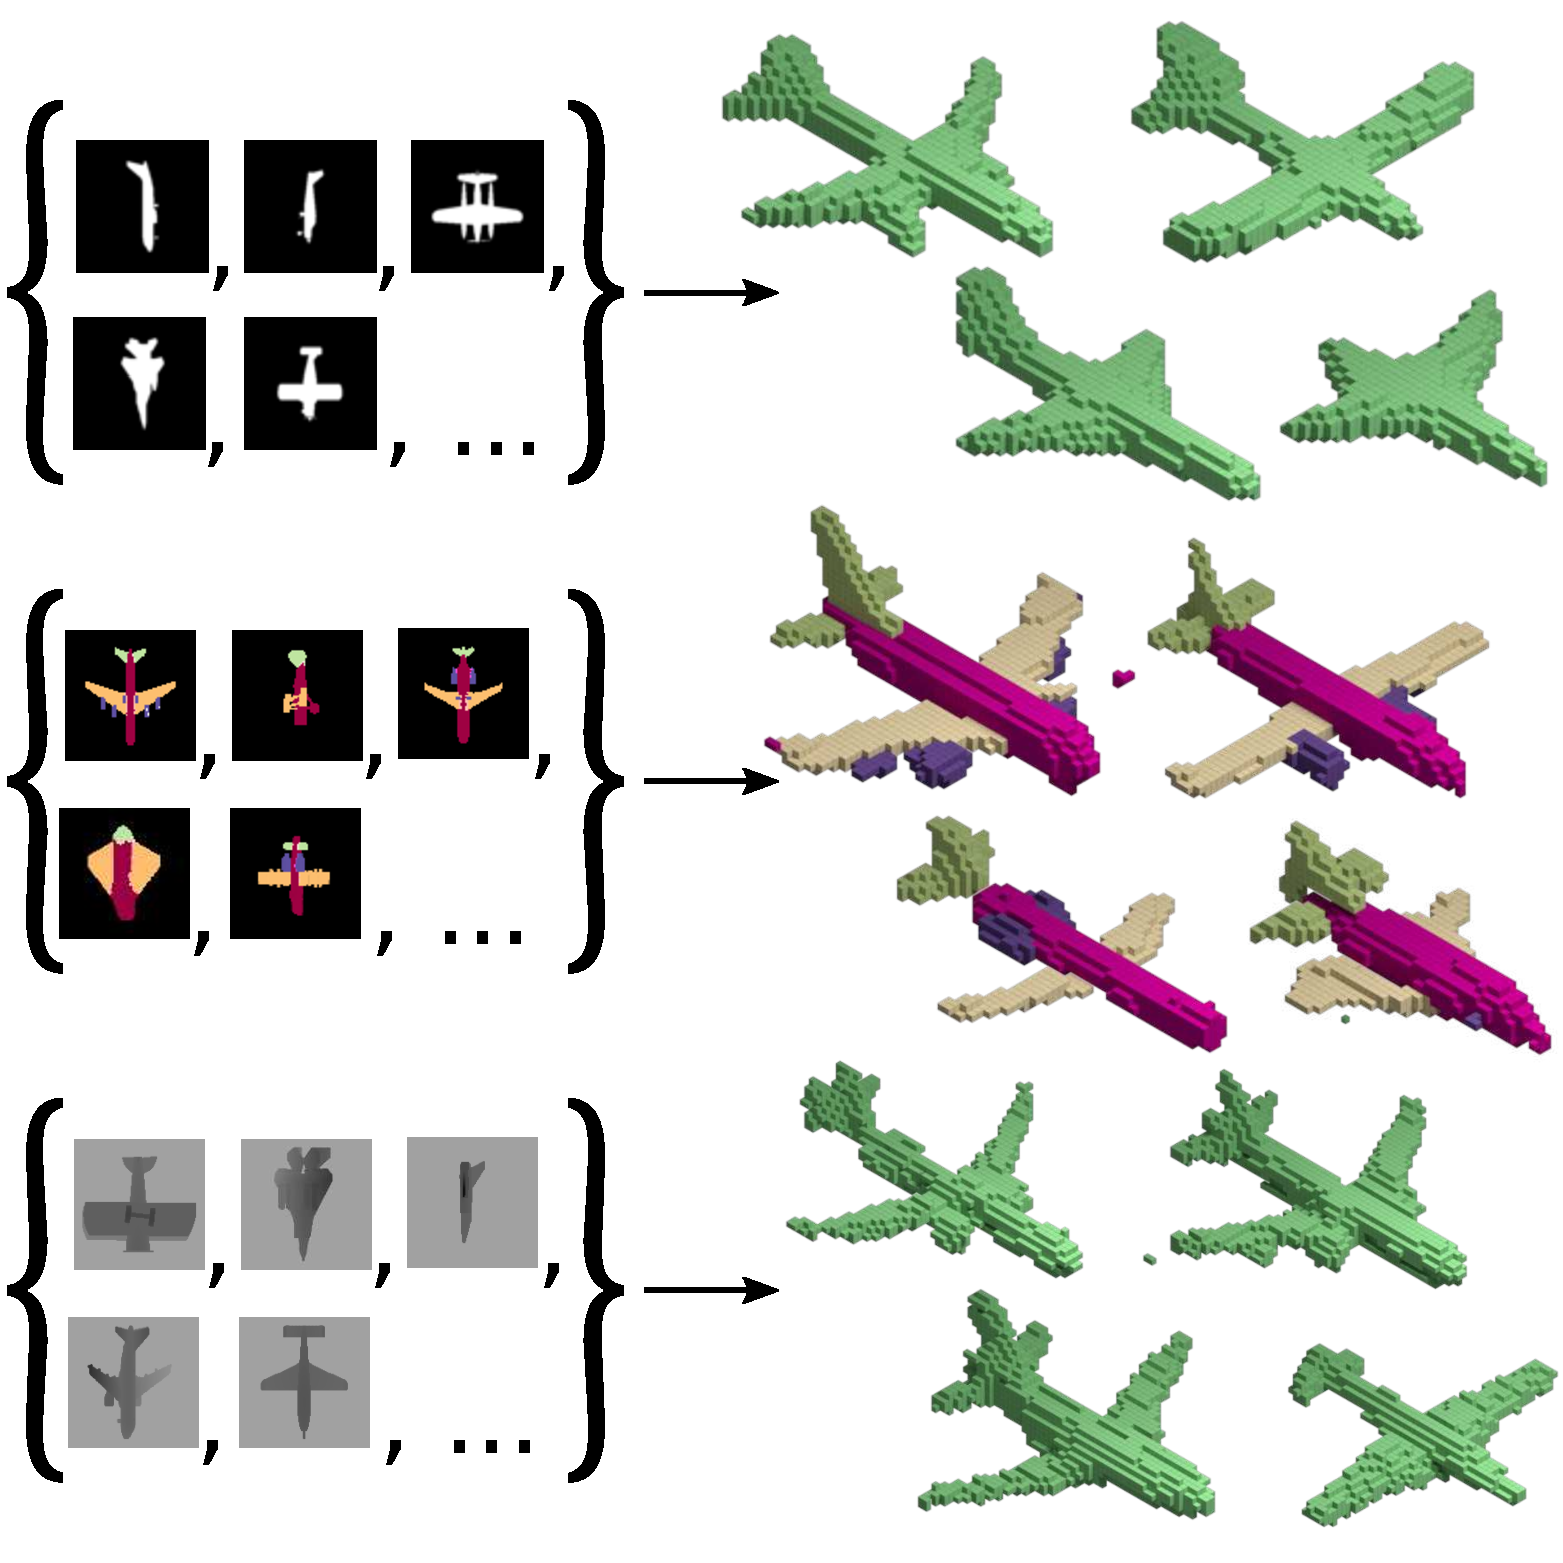
\includegraphics[width=1.0\linewidth]{fig/visabstract.pdf}
\caption{\label{f:problem} Our algorithm infers a generative model of
  the underlying 3D shapes given a collection of unlabeled images rendered as
  silhouettes, semantic segmentations or depth maps. 
	To the left, images representing the input dataset.
	To the right, shapes generated by the generative model trained with those images.}
\vspace{-12pt}
\end{figure}


The ability to infer 3D shapes of objects from their 2D views is one
of the central challenges in computer vision.
For example, when presented with a catalogue of airplane silhouettes
as shown in the top of Figure~\ref{f:problem}, one can mentally infer
their 3D shapes by simultaneously reasoning about the shape and
viewpoint variability.
In this work, we investigate the problem of learning a generative
model of 3D shapes from a collection of images of an unknown set of
objects within a category taken from an unknown set of views.
The images can be thought of as generalized projections of 3D shapes
into a 2D space in the form of silhouettes, depth maps,
or even part segmentations.
The problem is challenging as one is not provided with the information
about which object instance was used to generate each image, the viewpoint from
which each image was taken, the parameterization of the underlying shape
distribution, or even the number of underlying instances.
Hence, traditional techniques based on structure
from motion~\cite{hartley2003multiple,blanz1999morphable} or visual
hulls~\cite{laurentini1994visual}, cannot be directly applied.


We use the framework of generative adversarial
networks (GANs)~\cite{goodfellow2014generative} and augment the 3D shape
generator with a \emph{projection module}, as illustrated in Figure~\ref{fig:prgan-arch}.
The generator produces 3D shapes, the projection module
renders the shape from viewpoint sampled from a viewpoint distribution,
and the adversarial network discriminates real images from generated ones.
The projection module is a \emph{differentiable renderer} that allows us to map 3D
shapes to 2D images, as well as back-propagate the gradients of 2D
images to 3D shapes.
Once trained, the model can be used to infer 3D shape distributions
from a collection of images (Figure~\ref{f:problem} shows some samples
drawn from the generator), and to infer depth or viewpoint from a single
image, without using any 3D or viewpoint information during learning.
We call our approach \emph{projective generative adversarial network}
~(\prgan).








While there are several ways of rendering a 3D shape, we begin with a 
silhouette representation.
The motivation is that silhouettes can be easily
extracted when objects are photographed against clear backgrounds, such
as in catalogue images, but nevertheless they contain rich shape information.
Real-world images can also be used by removing background and converting them to
binary images. 
Our generative 3D model represents shapes using a voxel representation that indicates
the occupancy of a volume in a fixed-resolution 3D grid.
Our projection module is a feed-forward operator that
renders the volume as an image.
The feed-forward operator is differentiable, providing
the ability to adjust the 3D volume based on projections. 
Finally, we assume that the distribution over viewpoints
is known (assumed to be uniform in our experiments, but it could be any
distribution).

We then extend our analysis first presented in our earlier
work~\cite{prgan} by incorporating recent advances in training GANs and
designing projection modules to incorporate richer supervision.
The latter includes the availability of viewpoint information for
each image, depth maps instead of silhouettes, or semantic
segmentations such as part labels during learning.
Such supervision is easier to collect than acquiring full 3D scans of
objects.
For example, one can use a generic object viewpoint
estimator~\cite{su2015render} as weak supervision for our problem.
Similarly, semantic parts can be labeled on images directly and
already exist for many object categories such as airplanes, birds,
faces, and people.
We show that such information can be used to improve 3D reconstruction
by using an appropriate projection module.

To summarize our main contributions are as follows: (i) we propose
\prgan, a framework to learn probabilistic distributions over 3D
shapes from a collection of 2D views of objects. We demonstrate its
effectiveness on learning shape categories
such as chairs, airplanes, and cars sampled from online shape
repositories~\cite{chang2015shapenet,wu20153d}. 
The results are reasonable even when views from multiple categories
are combined; (ii) \prgan generates 3D shapes of comparable quality to GANs trained
directly on 3D data~\cite{wu2016learning};
(iii) The learned 3D representation can be used for unsupervised
estimation of 3D shape and viewpoint given a novel 2D shape, 
and for interpolation between two different shapes, (iv) Incorporating
additional cues as weak supervision improves the 3D shapes
reconstructions in our framework.



%% Enter your paper number here for the review copy
%\bmvcreviewcopy{200}

\chapter{Shape Generation using Spatially Partitioned Point Clouds}

%-------------------------------------------------------------------------
% Document starts here
%\begin{document}
%
%\maketitle
%
%\begin{abstract}
%
%We propose a method to generate 3D shapes using point clouds.
%Given a point-cloud representation of a 3D shape, our method builds a \emph{kd-tree} to spatially partition the points. This orders them consistently across all shapes, resulting in reasonably good correspondences across all shapes. % using the ordering of the leaf nodes. 
%We then use PCA analysis to derive a linear shape basis across the spatially partitioned points. Even with the spatial sorting, the point clouds are inherently noisy and the resulting distribution over the shape coefficients can be highly multi-modal. We propose to use the expressive power of neural networks to learn a distribution over the shape coefficients in a generative-adversarial framework. 
%Compared to 3D shape generative models trained on voxel-representations, our point-based method is considerably more light-weight and scalable, with little loss of quality. It also outperforms simpler linear factor models such as Probabilistic PCA, both qualitatively and quantitatively, on a number of categories from the ShapeNet dataset. Furthermore, our method can easily incorporate other point attributes such as normal and color information, an additional advantage over voxel-based representations.
%\end{abstract}
%

\def\point{P}
\def\matrix{P}
\def\npoints{N}
\def\nshapes{S}
\def\nbasis{B}

\section{Introduction}\label{sec:intro}
The choice of representation is a critical for learning a good generative model of 3D shapes. Voxel-based representations that discretize the geometric occupancy into a fixed resolution 3D grid offers compelling advantages since convolutional operations can be applied. 
However, they scale poorly with the resolution of the grid and are also wasteful since the geometry of most 3D shapes lies on their surfaces, resulting in a voxel grid that's mostly empty, especially at high resolutions. 
Surface-based representations such as triangle meshes and point clouds are more efficient for capturing surface geometry, but these representations are inherently unstructured -- because there is no natural ordering of the points, they are better expressed as an unordered \emph{set}. Consequently, unlike \emph{ordered} representations, they are cannot be easily generated using existing deep convolutional architectures. 
The exception is when the points are in perfect correspondence across shapes, in which case a linear shape basis can be effective (\eg, for faces or human bodies). However estimating accurate global correspondences is difficult and even poorly defined for categories such as chairs that have complex and varying geometry. Thus generating 3D shapes as point clouds remains a challenge.


We propose a new method for learning a generative model for 3D shapes represented as point clouds. Figure~\ref{fig:arch} illustrates our network architecture. 
The key idea is to use a space-partitioning data structure, such as a \emph{kd-tree}, to approximately order the points. 
Unlike a voxel-grid occupancy representation, the kd-tree representation scales linearly with the number of points on the surface and can adapt to the geometry of the model.
Moreover one can easily incorporate other point attributes such as surface normal, color, and texture coordinates into this representation, making it possible to generate new shapes that automatically include these information.
We learn a shape basis over the ordered point clouds using low-rank factorization of the shape coordinates. 
%The point cloud for each shape is optionally reordered such that the distance to the manifold spanned by the shape basis is minimized. 
%Subsequently a new shape basis can be learned on the reordered points and the process iterated till convergence.
If the alignments induced by the kd-tree sorting was perfect, the distribution of the coefficients would be simple.
Indeed this is the assumption behind generative models such as Probabilistic PCA~\cite{tipping1999probabilistic} that models the distributions of coefficients using independent Gaussians. 
However, imperfect alignment can lead to a multi-modal and heavy-tailed distribution over the coefficients.
To address this issue, we propose to leverage the expressive power of neural networks and employ a Generative Adversarial Network (GAN)~\cite{goodfellow2014generative} to learn the distribution over the shape coefficients.
Unlike other non-parametric distributions such as a mixture of Gaussians, the GAN linearizes the distribution of shapes and allows interpolation between them using arithmetic operations.
At the same time our method remains light-weight and scalable, since most shape categories can be well represented with a hundred basis coefficients.


\begin{figure}
\centering
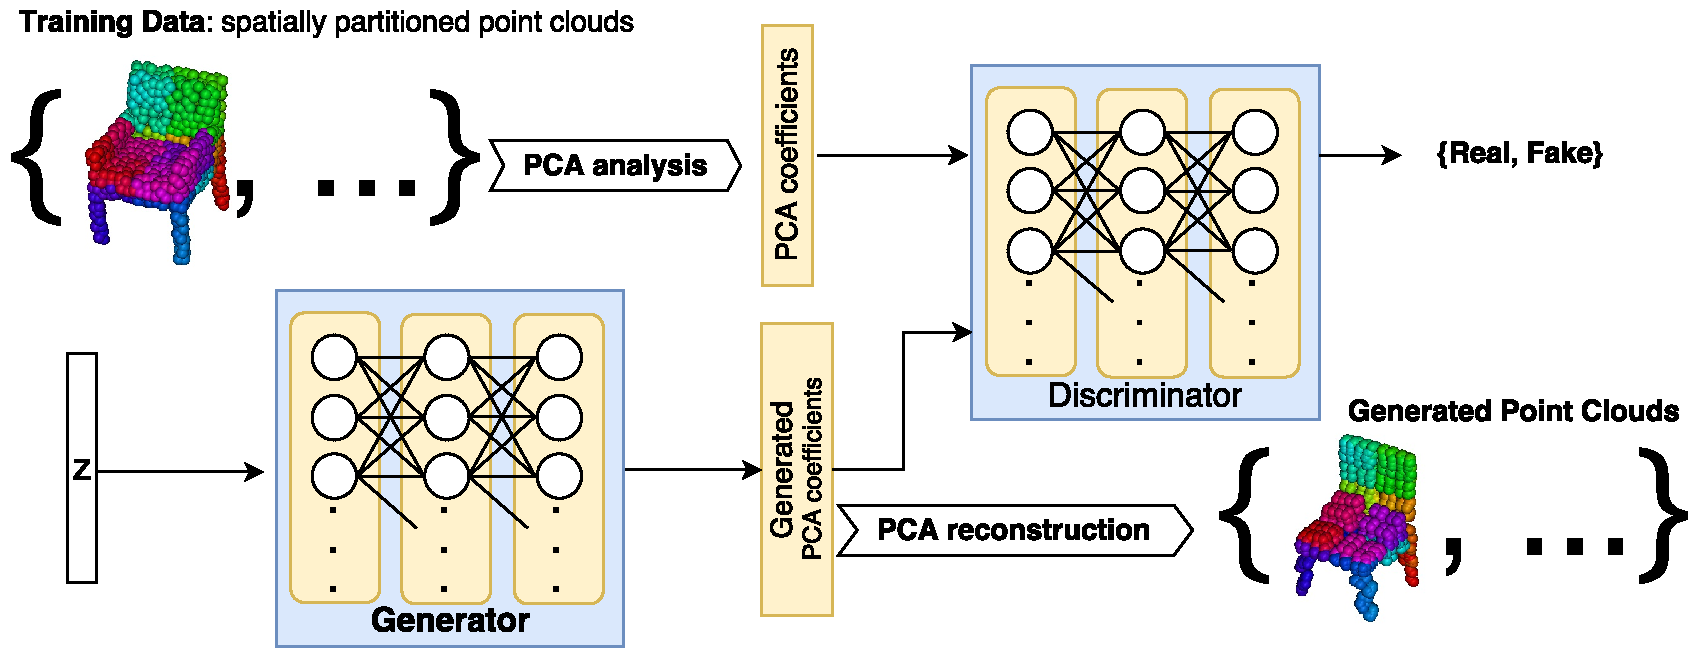
\includegraphics[width=0.8\linewidth]{PCAGAN/images/PCAGAN_architecture.pdf}
\caption{\small \label{fig:arch} Our network architecture for generating 3D shapes using spatially partitioned point clouds. We perform PCA analysis on the training data to drive a shape basis and associated shape coefficients. We then train a GAN to learn the multi-modal distribution over the coefficients. The generated coefficients are combined with the shape basis to produce the output point clouds.}
\vspace{-12pt}
\end{figure}

We compare the proposed generative model to a 3D-GAN approach of Wu~\etal~\cite{wu2016learning} that learns a convolutional architecture over a voxel-representation of 3D shapes. In addition we compare to a Probabilistic PCA (PPCA) baseline using the same point-cloud representation. Experiments on several categories in the ShapeNet dataset show that the proposed approach outperforms PPCA and 3D-GAN, quantitatively and qualitatively. Compared to the 3D-GANs our models are an order-of-magnitude faster and smaller. We then present several experiments evaluating the role of the kd-tree on the quality of the generated shapes. We also show that a 1D-convolutional GAN trained on the ordered list of point coordinates produces samples of reasonable quality, suggesting that the kd-tree ordering plays a key role.


\vspace{-12pt}
\section{Related Work}\label{sec:related}

\noindent \textbf{Generative models for 3D shapes.} Recently, Wu~\etal in~\cite{wu2016learning} proposed a generative model of 3D shapes represented by voxels, using a variant of GAN adapted to 3D convolutions. Two other works are also related. Rezende~\etal~\cite{rezende2016unsupervised} show results for 3D shape completion for simple shapes when views are provided, but require the viewpoints to be known and the generative models are trained on 3D data. Yan~\etal in~\cite{yan2016perspective} learn a mapping from an image to 3D using multiple projections of the 3D shape from known viewpoints (similar to a visual-hull
technique). However, these models operate on a voxel representation of 3D shape, which is difficult to scale up to higher resolution. The network also contains a large number of parameters, which are difficult and take a long time to train. Our method uses spatially partitioned point cloud to represent each shape. It is considerably more lightweight and easy to scale up. In addition, by using a linear shape basis, our network is small hence much easier and faster to train. Through experiments we show that the benefits of this lightweight approach come with no loss of quality compared to previous work. Several recent techniques~\cite{tatarchenko2017octree,Riegler2017CVPR} have explored multi-resolution voxel representations such as \emph{octrees}~\cite{meagher1982geometric} to improve their memory footprint at the expense of additional book keeping. But it remains unclear if 3D-GANs can generate high-resolution sparse outputs.

\vspace{8pt}
\noindent \textbf{Learning a 3D shape bases using point-to-point correspondence.} Another line of work aims to learn a shape basis from data assuming a global alignment of point clouds across models. 
Blanz and Vetter in~\cite{blanz1999morphable} popularized the 3D morphable models for faces which are learned by a PCA analysis of the point clouds across a set of faces with known correspondences. 
The same idea has also been applied to human bodies~\cite{allen2003space}, and other deformable categories~\cite{kar2015category}. 
However, establishing the point-to-point correspondence between 3D shapes is a challenging problem. 
Techniques are based on global rigid or non-rigid pairwise alignment (\eg, \cite{besl1992method,chen1992object,bronstein2010gromov}), learning feature descriptors for matching (\eg, techniques in this survey~\cite{van2011survey}), or fitting a parametric model to each instance (\eg,~\cite{cashman2013shape,prasad2010finding}).
Some techniques improve pairwise correspondence by enforcing cycle-consistency across instances~\cite{huang2013consistent}. 
However, none of these techniques provide consistent global correspondences for shapes with varying and complex structures (\eg, chairs and airplanes). 
Our method uses spatial sorting based on a kd-tree structure. It is a fast and lightweight approximation to the correspondence problem. However, unlike alignment-based approaches, one drawback of the kd-tree sorting is that it's not robust to rotations of the model instances. This is also a drawback of the voxel-based representations.
The ShapeNet dataset~\cite{chang2015shapenet} used in our experiments already contains objects that are consistently oriented, but otherwise one can apply automatic techniques (\eg,~\cite{Su_2015_ICCV}) for viewpoint estimation to achieve this.

\vspace{8pt}
\noindent \textbf{Representing shapes as sets.} Another direction is to use loss functions over \emph{sets} such as Chamfer, Hausdroff, or Earth Mover's Distance (EMD) to estimate similarity between models. The recent work of Fan~\etal~\cite{fan2016point} explores this direction and trains a neural network to generate points from a single image by minimizing the EMD between the generated points and the model points. To apply this approach for shape generation one requires the evaluation of the loss of a generated shape with respect to a distribution of target shapes. While this can be approximated by computing statistics of EMD distance of the generated shape to all shapes in the training data, this is highly inefficient since EMD computation alone scales cubically with the number of points. 
Thus training neural architectures to generate and evaluate loss functions over sets efficiently remains an open problem. 
The approximate ordering induced by the kd-tree allows efficient matrix operations on the \emph{ordered} vector of point coordinates for training shape generators and discriminators.

\section{Method}\label{pca:method}

\begin{figure}
\centering
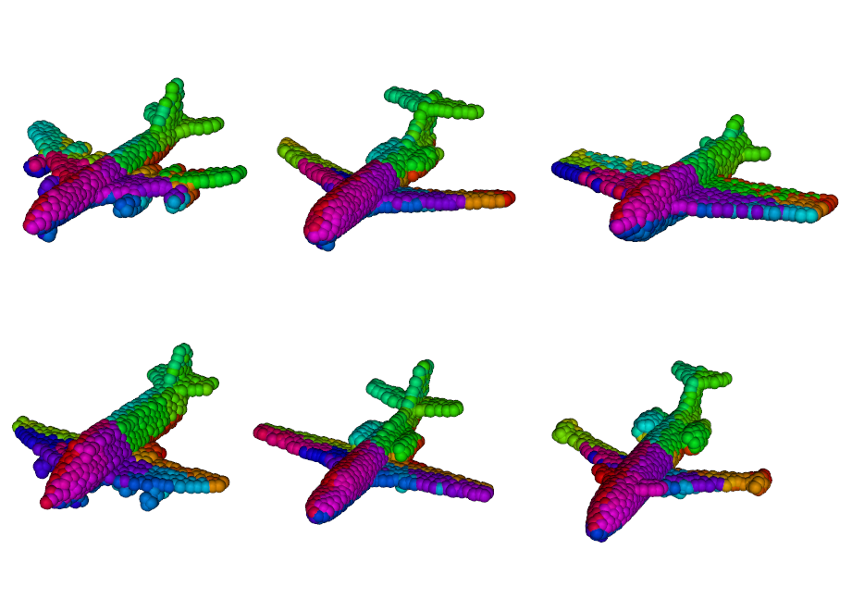
\includegraphics[width=0.49\linewidth]{PCAGAN/images/airplanes_sorting_new2.png}

\includegraphics[height=1.4in]{PCAGAN/images/vline.png}
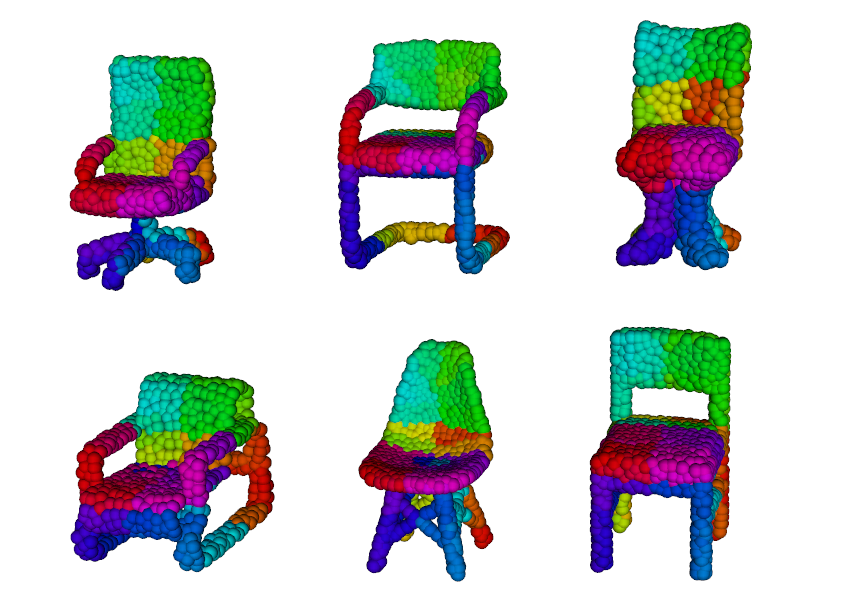
\includegraphics[width=0.49\linewidth]{PCAGAN/images/chairs_sorting.png}
\vspace{-12pt}
\caption{\small \label{fig:point_sorting} Visualization of spatially partitioned points for six training shapes from each category. Every point is colored by its index in the sorted order. This shows that the kd-tree sorting leads to reasonably good correspondences between points across all shapes.}
\vspace{-12pt} 
\end{figure}

This section explains our method. To begin, we sample each training 3D shape using Poisson Disk sampling~\cite{Bowers:2010:PPD} to generate a consistent number of evenly distributed points per shape. We typically sample each shape with 1K points, and this can be easily increased or decreased based on actual need. We then build a kd-tree data structure for each point cloud to spatially partition the points and order them consistently across all shapes. Next, we compute the PCA bases using all the point data. 
%The ordering of points in each shape can be further refined by iteratively swapping points to minimize the PCA reconstruction error.
Finally, we train a GAN on the shape coefficients to learn the multi-modal distribution of these coefficients and use it to generate new shapes.

\vspace{4pt}
\noindent \textbf{Spatially partitioned point cloud.} We use $\{\point_i^s\}$ to represent a point cloud where $i$ is the point index and $s$ is the shape index. By default the point data $\point$ includes the $x,y,z$ coordinates of a point, but can include additional attributes such as normal and color etc. We assume each point cloud is centered at the origin and the bounding box is normalized so that the longest dimension spans [-0.5, 0.5]. For each point cloud we build a kd-tree by the following procedure: we start by sorting the entire point cloud along the $x$-axis, and split it in half, resulting in a left subset and a right subset; we then recursively split each of the two subsets, but this time along the $y$-axis; then along $z$-axis, and so on. Basically it's a recursive splitting process where the splitting axis alternates between $x$, $y$, and $z$. The splitting axes can also be chosen in other ways (such as using the longest dimension at each split) to optimize the kd-tree building, but it needs to be consistent across all point clouds.

The kd-tree building naturally sorts the point cloud spatially, and is consistent across all shapes. For example, if we pick the first point from each sorted point cloud, they all have the same spatial relationship to the rest of the points. As a result, this establishes reasonably good correspondences among the point clouds. Figure~\ref{fig:point_sorting} shows an illustration.

%\vspace{4pt}
\noindent \textbf{Computing PCA bases.} We use PCA analysis to derive a linear shape basis on the spatially partitioned point clouds. To begin, we construct a matrix $\matrix$ that consists of the concatenated $x,y,z$ coordinates of each point cloud and all shapes in a given category. The dimensionality of the matrix is $3\,\npoints\times\nshapes$ where $\npoints$ is the number of points in each shape, and $\nshapes$ is the number of shapes. We then perform a PCA on the matrix: $\matrix=U \Sigma V$, resulting in a linear shape basis $U$. Thanks to point sorting using kd-tree, a small basis set is sufficient to well represent all shapes in a category. We use $\nbasis$ to represent the size of the shape basis, and by default choose $\nbasis=100$, which has worked well for all ShapeNet categories we experimented with. The choice of $\nbasis$ can be observed from the rapid dropping of singular values $\Sigma$ following the PCA analysis. Without a good spatial sorting method, it would require a significantly larger basis set to accurately represent all shapes.

To include other point attributes, such as normal, we can concatenate these attributes with the $x,y,z$ coordinates. For example, a matrix that consists of both point and normal data would be $6\,\npoints\times\nshapes$ in size. We suitable increase the basis size (e.g. by choosing $\nbasis=200$) to accommodate the additional data. The rest of the PCA analysis is performed the same way.

%\paragraph{Optimizing point ordering.} While sorting using the kd-tree creates good initial correspondences between points one can further optimize the point ordering by iteratively reducing the PCA reconstruction error.

%\vspace{4pt}
\noindent \textbf{Learning shape coefficients using GAN.} Our method employs a GAN to learn the distribution over the shape coefficients. % on the PCA basis computed in the above step.
Following the PCA analysis step, the matrix $V$ captures the coefficients for all training shapes, i.e. the projections of each point cloud onto the PCA basis. It provides a compact and yet accurate approximation of the 3D shapes. Therefore our generative model only needs to learn to generate the shape coefficients. 
%we can project the point clouds in our training data into this basis and have a compact representation for each one of our training samples.
%In other words, instead of learning how to generate a complete point cloud, our model only has to learn how to generate the coefficients obtained by projecting the point cloud in a linear basis.
Since the dimensionality of the shape basis ($\nbasis=100$) is much smaller (than the number of points on each shape), we can train a GAN to learn the distribution of coeffcients using
a simple and lightweight architecture. In our setup, the random encoding $z$ is a 100-D vector. The generator and discriminator are both fully connected neural networks consisting of 4 layers each, with 100 nodes in each layer.
Each layer is followed by a batch normalization step.
Following the guidelines of previous architectures \cite{wu2016learning}, our discriminator
uses a LeakyReLU activation while our generator uses regular ReLU.



The discriminator is trained by minimizing the vanilla GAN loss described as follows:
\begin{equation}\label{eqn:gan}
	\mathcal{L}_d = \mathbb{E}_{x\sim{\cal T}} [ \log \left(D(x)\right) ] + \mathbb{E}_{z\sim U} [ \log \left(1-D(G(z))\right) ].
\end{equation}
where $x$ represents the shape coefficients, $D$ is the discriminator, $G$ is the generator, $U$ represents an uniform distribution of real numbers in $(-1, 1)$,
and $\mathcal{T}$ is the training data.
In our experiments, we noticed that using the traditional loss for the generator leads to a highly
unstable training where the generated data converges to a single mode (which loses diversity).
To overcome this issue, we employ an approach similar to the one proposed in \cite{improvedGAN}.
Specifically, let $f(x)$ be the intermediate activations of the discriminator given an input $x$.
Our generator will try to generate samples that match some statistics of the activations of
the real data, namely mean and covariance.
Thus, the generator loss is defined as follows:
\begin{equation}\label{eqn:generator}
	\mathcal{L}_g = \norm{\mathbb{E}_{x\sim{\cal T}} [ f(x) ] - \mathbb{E}_{z\sim U} [ f(G(z)) ]}_2^2 +
					\norm{cov_{x\sim{\cal T}} [ f(x) ] - cov_{z\sim U} [ f(G(z)) ]}_2^2
\end{equation}
where $cov$ is the vectorized covariance matrix of the activations.
Using this loss results in a much more stable learning procedure.
During all our experiments the single mode problem never occurred, even when
training the GAN for thousands of epochs.
We use the Adam optimizer~\cite{Adam} with a learning rate of $10^{-4}$ for the discriminator and $0.0025$ for the
generator.
Similarly to \cite{wu2016learning}, we only train the discriminator if its accuracy is below 80\%.

\begin{figure}[t]
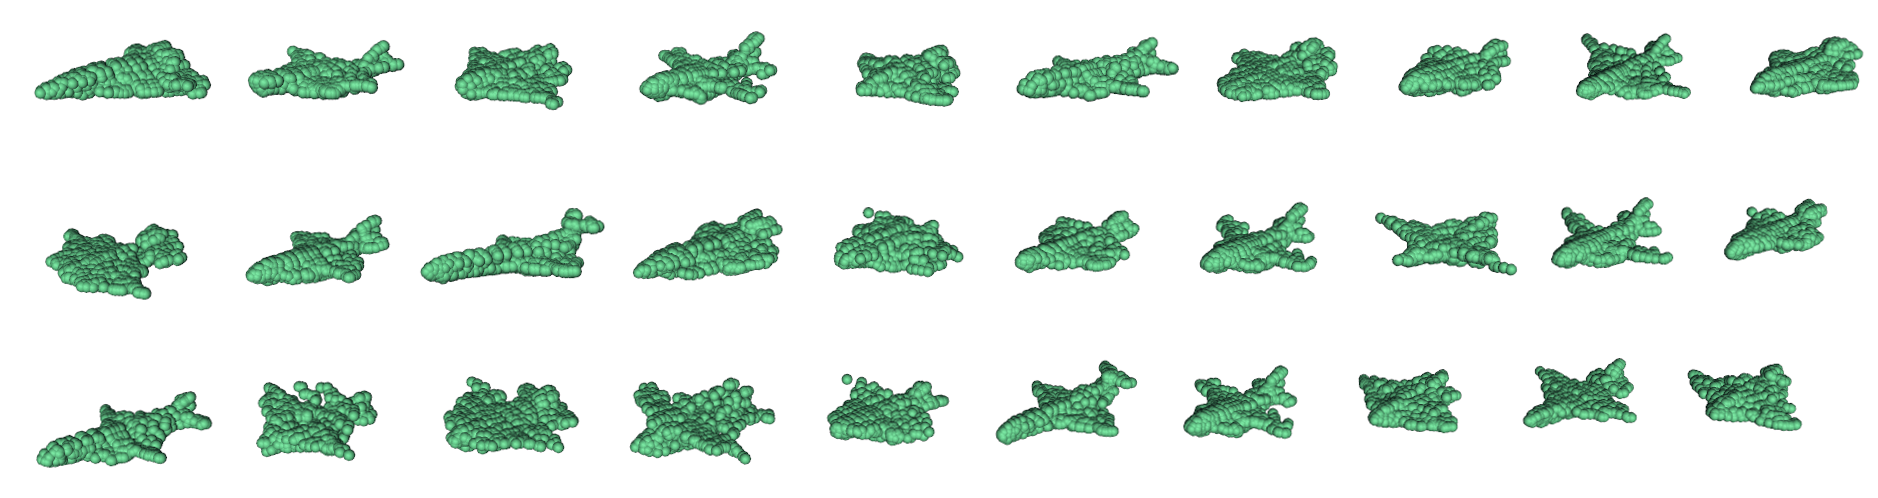
\includegraphics[width=1.0\linewidth]{PCAGAN/images/gallery/airplanes.png}

\includegraphics[width=1.0\linewidth]{PCAGAN/images/hline.png}
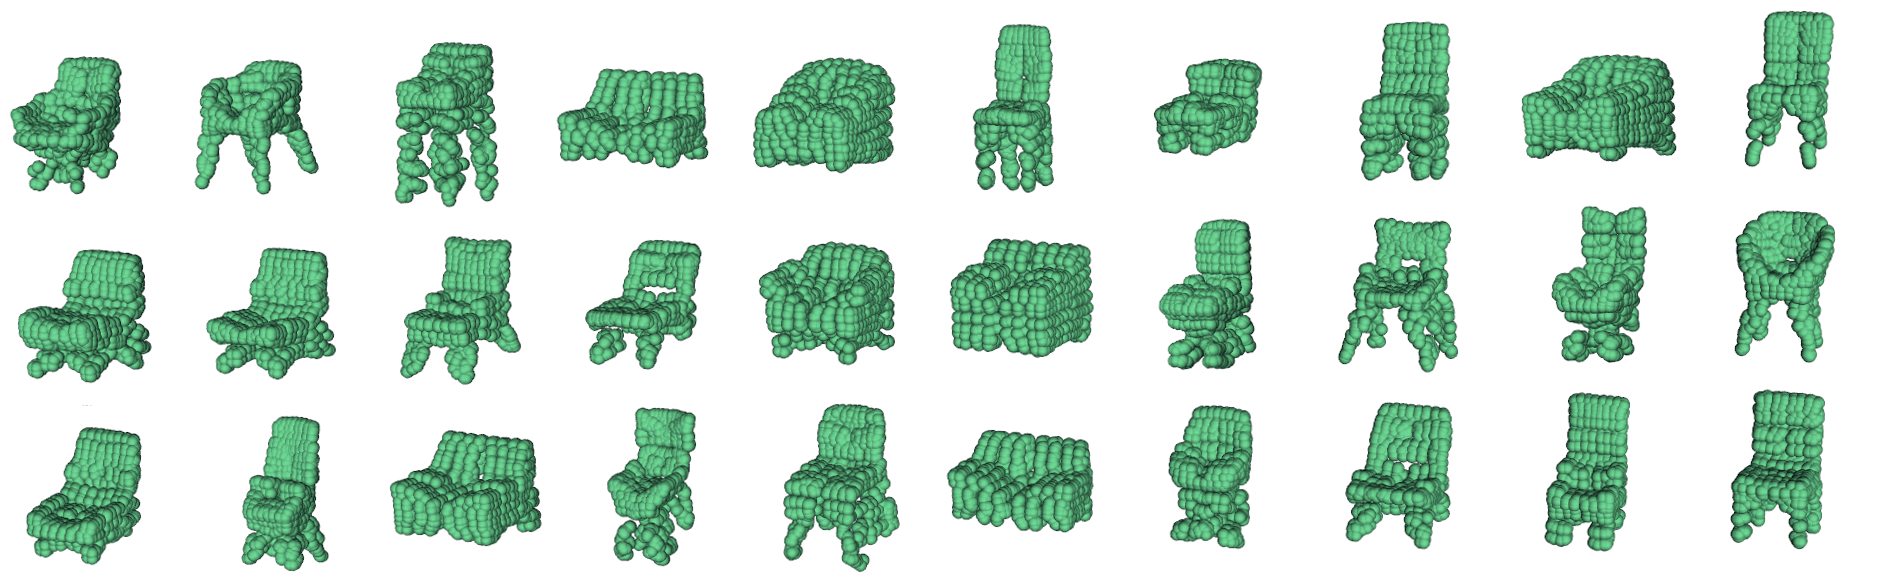
\includegraphics[width=1.0\linewidth]{PCAGAN/images/gallery/chairs.png}

\includegraphics[width=1.0\linewidth]{PCAGAN/images/hline.png}
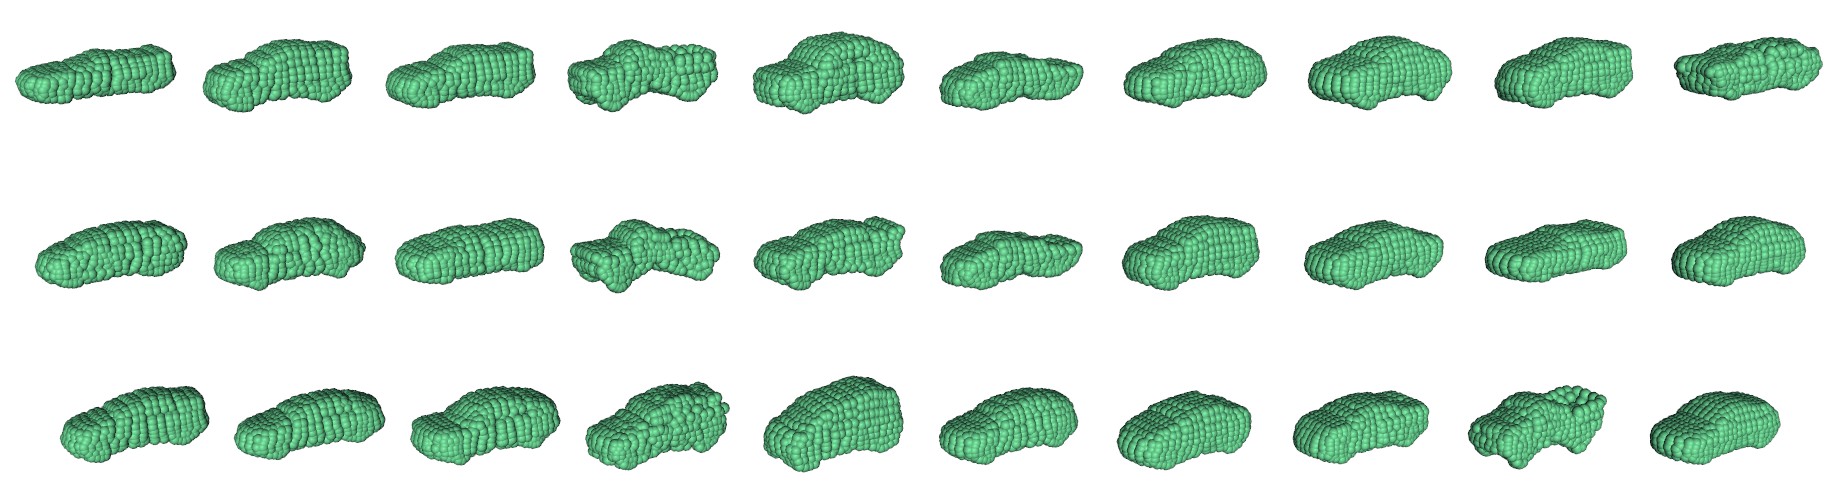
\includegraphics[width=1.0\linewidth]{PCAGAN/images/gallery/cars.png}
\vspace{-16pt}
\caption{\small \label{pca:gallery} A gallery showing results of using our method to generate points clouds for three categories: airplane, chair, and car. We use our method to train a GAN for each category separately. The training is generally very fast and completes within a few minutes. The results shown here are generated by randomly sampling the encoding $z$ of the GAN.}
\vspace{-12pt}
\end{figure}




\begin{figure}[t]
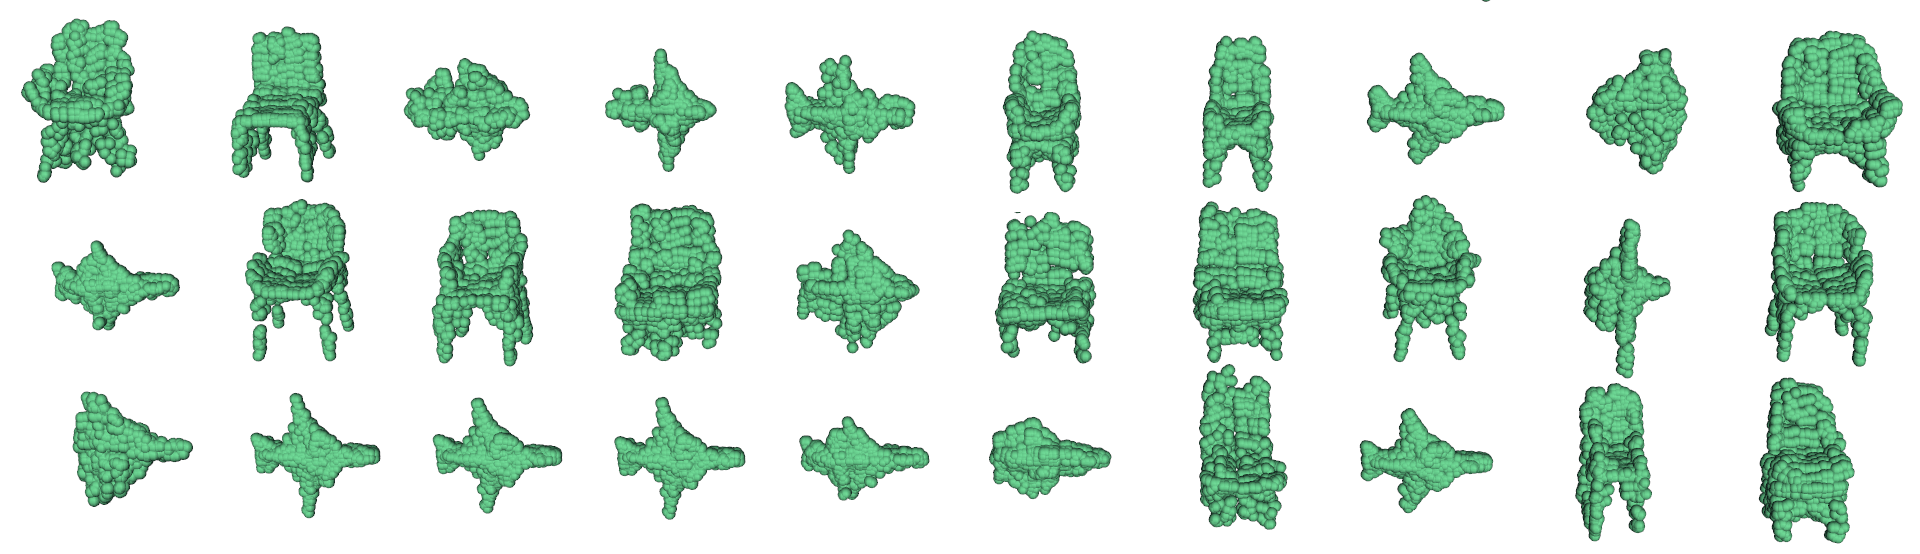
\includegraphics[width=1.0\linewidth]{PCAGAN/images/gallery/chairs_airplane.png}
\vspace{-16pt}
\caption{\small \label{fig:mixed} Results for a mixed category (chair + airplane) showing the ability of our method to capture multi-modal distributions over mixed-category shapes.}
\vspace{-6pt}
\end{figure}

\begin{figure}[t]
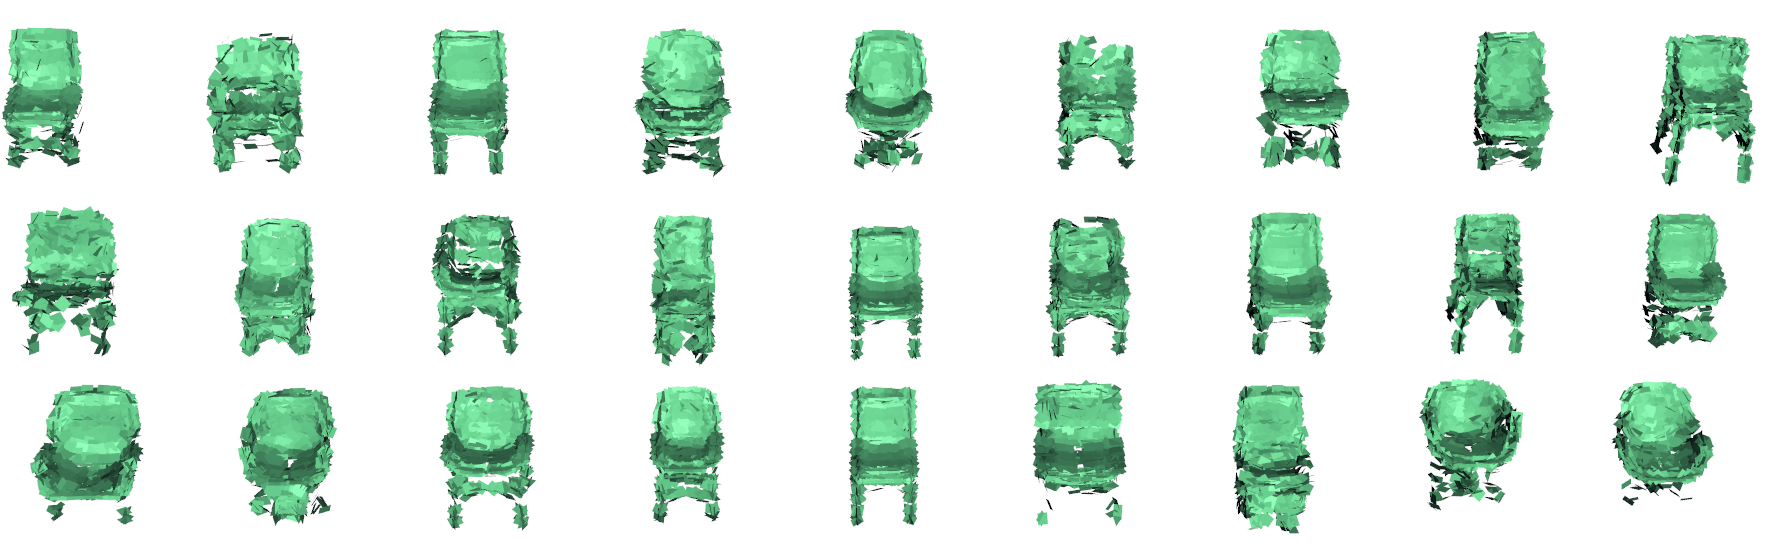
\includegraphics[width=1.0\linewidth]{PCAGAN/images/gallery/chairs_normals.png}
\vspace{-16pt}
\caption{\small \label{fig:normals} Chairs generated with normal. For visualization we shade each point as a square patch centered at the point and oriented by the normal. This shows the ability of our method to generate not only $x,y,z$ coordinates but also incorporate associated point attributes such as normal.}
\vspace{-12pt}
\end{figure}

\section{Experiments}\label{sec:experiments}

\noindent \textbf{Training data.} To generate training data, we use several shape categories from the ShapeNet dataset~\cite{chang2015shapenet}, including chairs, airplanes, cars etc. We sample each shape with 1K Poisson disk sample points using the algorithm described in~\cite{Bowers:2010:PPD}. Poisson disk samples evenly disperse the points over the surface, which turns out to work better at preserving geometric details than using white noise samples. We can easily increase the number of sample points to 4K or 8K and beyond. Unlike voxel-based representations, our method is lightweight, and increasing the sample size only leads to moderate increases in computation resources and time. 

%Those points are sampled in a blue-noise pattern and sorted using the space-partitioning method described in the previous Section.
%Our experiments show that blue-noise sampled points perform slightly better when representing objects with finer geometric details. Each one of the point clouds used in our experiments contain 1024 points.

\vspace{12pt}
\noindent \textbf{Qualitative evaluation.} Figure~\ref{pca:gallery} shows a gallery of results generated using our method for each of the three categories: airplane, chair, and car. The results are generated by randomly sampling the encoding $z$ and demonstrate a variety of shapes within each category. The training is very fast and generally completes within a few minutes. This is an order of magnitude faster than training deep neural networks built upon voxel representations. Figure~\ref{fig:mixed} shows additional results for a mixed category that combines shapes from the chair and airplane datasets. For this mixed category we used $B=300$ basis. The results show the ability of our method to capture the multi-modal distributions over mixed-category shapes.

\vspace{12pt}
\noindent \textbf{Generating multiple point attributes.} Our method can generate points with multiple attributes, such as surface normal, color, by simply appending these attributes to the $(x,y,z)$ coordinates. The overall procedure remains the same except the shape basis is learned over the joint space of positions and normals etc. Figure~\ref{fig:normals} shows chair results generated with normal. The ability to incorporate point attributes is an additional advantage over voxel-based representations (which do not explicitly represent surface information of shapes).

%In the following we present several quantitative and qualitative results to evaluate the our method.
%We start by presenting a quantitative comparison between our model and a competitive PPCA baseline which,
%using the space-partitioning scheme proposed in this paper, yields a similar perceptual quality to 3D-GAN~\cite{wu2016learning}
%as can be observed in Figure~\ref{fig:comparison}.
%We also use this experiment to demonstrate the effect of the number of basis in the generated shapes.
%Second, we present a qualitative evaluation of our technique by using the same training data to query the closest model between
%shapes generated by our method, PPCA and 3D-GAN.
%Third, we show that the GAN learns a manifold of the point clouds by displaying plausible shapes generated while interpolating
%the generator encoding.
%Finally, we demonstrate the ability of our method to generate different types of 3D shapes: chairs, airplanes, cars, tables and
%even multiple categories using same model.
%We also show results where the point clouds are generated with normal annotation.

\begin{table}[t]
\centering
\begin{tabular}{c|ccc|c}
Dataset & GAN(10) & GAN(50) &	GAN(100) &	PPCA (100) \\
\hline
Chairs	& 2.57	& 2.53	& \textbf{2.37}	& 2.88 \\
Airplanes	& 1.96	& \textbf{1.93}	& 1.94	& 2.29 \\
Cars	& 1.45	& \textbf{1.42}	& 1.44	& 1.59 \\
Tables	& 2.88	& 2.68	& \textbf{2.66}	& 3.18 \\
\end{tabular}
\caption{\small \label{tab:quant} Distance (Eq.\ref{eq:chamfer-distance}) between the generated samples and training samples for different generative models. The numbers in parentheses indicate the number of PCA coefficients used for each column. The GAN approach outperforms the PPCA baseline by a considerable margin.}
\vspace{-6pt}
\end{table}

\begin{figure}[t]
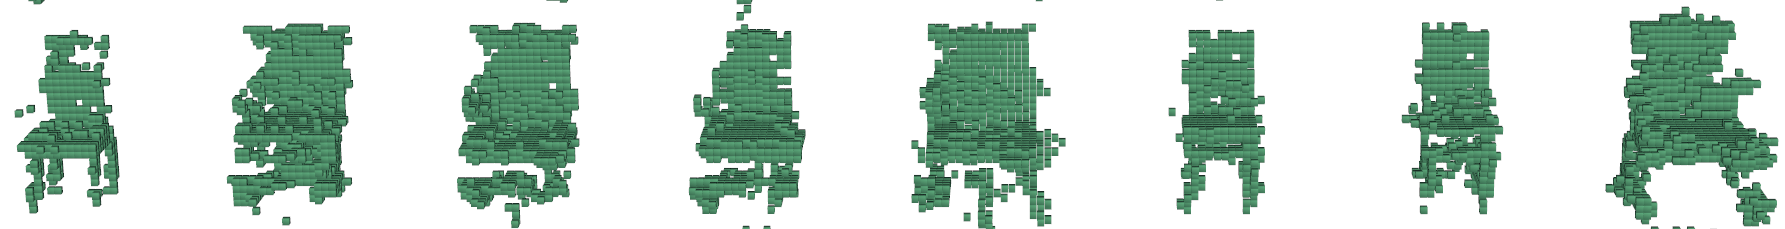
\includegraphics[width=1.0\linewidth]{PCAGAN/images/3DGAN_batch1row.png}
\vspace{-16pt}
\caption{\small \label{fig:3dgan} 3D-GAN result for the chair category. The models are generated by following~\cite{wu2016learning}.}
\vspace{-12pt}
\end{figure}

\begin{figure}[t]
\centering
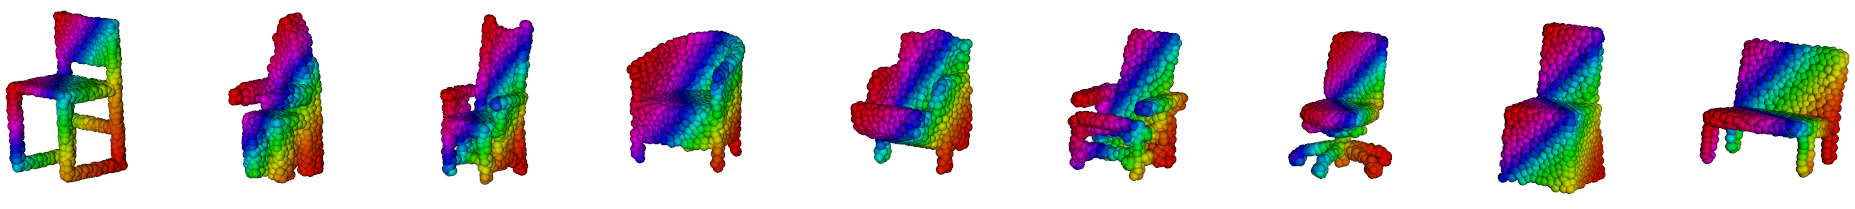
\includegraphics[width=0.8\linewidth]{PCAGAN/images/chairs_xyz_data.png}
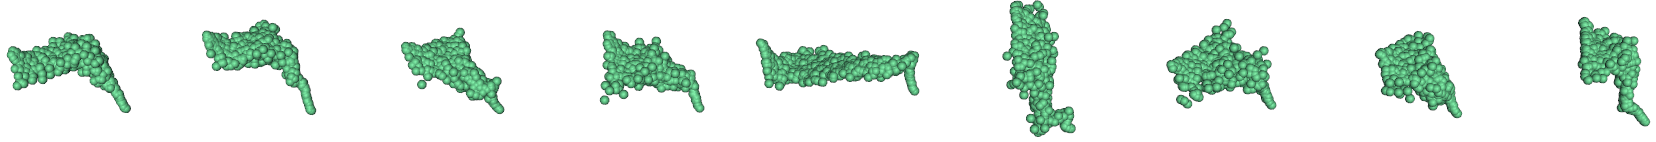
\includegraphics[width=0.8\linewidth]{PCAGAN/images/chairs_xyz_generated.png}
\vspace{-8pt}
\caption{\small \label{fig:chairsxyz} Sorting point clouds using $x+y+z$ values. Top row shows a visualization of the training data using this sorting strategy.
	Bottom row shows the generated shapes for the chair category. They are visually of poor quality compared to kd-tree sorting.}
\vspace{-6pt}	
\end{figure}

\begin{figure}[t]
\centering
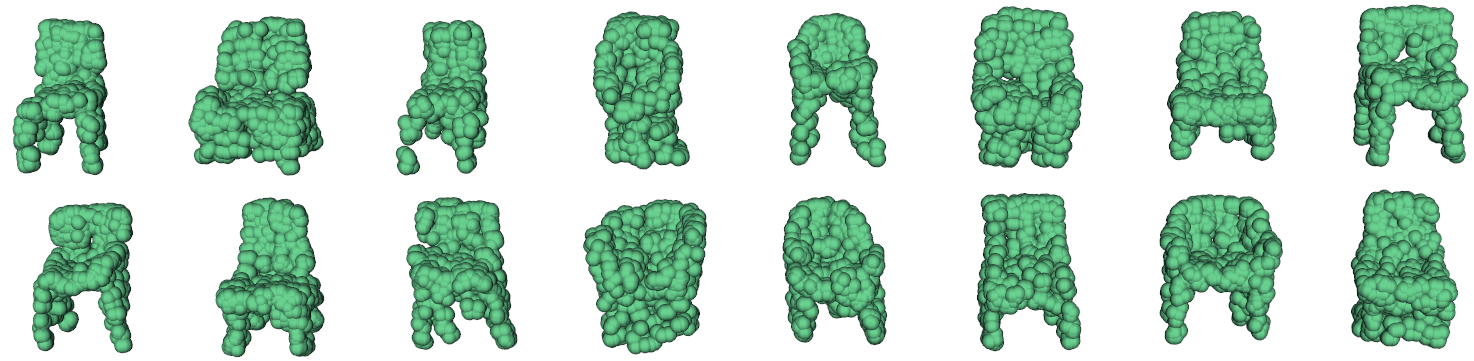
\includegraphics[width=0.8\linewidth]{PCAGAN/images/chairs_1dconv.png}
\caption{\small \label{fig:1dconv} Samples from an alternative GAN architecture using 1D convolutions. Trained using the the point clouds directly.}
\vspace{-12pt}
\end{figure}


\vspace{12pt}
\noindent \textbf{Quantitative evaluation.}
We compare variations of our model to a PPCA baseline~\cite{tipping1999probabilistic}. The PPCA model performs a linear factor analysis of the data using: $y \sim \mathbf{W}x + \mu + \sigma$. The matrix $\mathbf{W}$ is a basis, the latent variables $x \sim N(0, I)$, noise $\sigma \sim N(0, \sigma^2I)$ and the $\mu$ is the data mean. In other words, PPCA learns an independent Gaussian distribution over the coefficients $x$, whereas our approach employs a GAN. We compare PPCA results with variations of our model by changing the number of basis and examining its influence on the quality of the results.
The metric used in the evaluation is defined as follows.
Let $\mathcal{T}$ and $\mathcal{S}$ be the set of training and generated samples, respectively.
We define our distance measure $d(\mathcal{T}, \mathcal{S})$ using a variant of the Chamfer distance, as follows:
\begin{equation}\label{eq:chamfer-distance}
	d(\mathcal{T}, \mathcal{S}) = 
	\frac{1}{|\mathcal{T}|} \sum_{t \in \mathcal{T}} \min_{s \in \mathcal{S}} \norm{t - s}_2 +
	\frac{1}{|\mathcal{S}|} \sum_{s \in \mathcal{S}} \min_{t \in \mathcal{T}} \norm{t - s}_2
\end{equation}
The results can be seen in Table~\ref{tab:quant}. Our approach that uses a GAN to model the distribution of coefficients consistently outperforms the PPCA baseline, which models the distribution as a Gaussian. For the chairs and tables categories the difference between the PPCA and GAN is large, suggesting that the distribution of the coefficients is highly multi-modal. The results by varying the number of bases are also shown in the Table~\ref{tab:quant}. Increasing the number of basis beyond a hundred did not improve our results further.


\vspace{12pt}
\noindent \textbf{Visual comparison to 3D-GAN.} To compare our results with the 3D-GAN model~\cite{wu2016learning}, we followed their description to implement our own version of the algorithm as there is no publicly available implementation that can be trained from scratch. Figure~\ref{fig:3dgan} shows the 3D-GAN results for the chair category. As in~\cite{wu2016learning}, the training data is generated by voxelizing each shape to $64^3$ resolution, and we employ the same hyper-parameters for our GAN model as theirs. Our results, which can be found in Figure~\ref{pca:gallery}, compare favorably to 3D-GAN. In addition, our network is significantly smaller and faster to train.

%shows a set of samples drawn from the generative model for chair category. Visually the results are of better quality than the 3D-GAN and PPCA. However a quantitative comparison with 3D-GAN is difficult since the shape is represented in different ways.


\vspace{12pt}
\noindent \textbf{The role of the \emph{kd-tree}.} The kd-tree induces a shape-dependent but consistent ordering of points across shapes. Moreover the ordering is locality preserving, i.e., two points that are close in the underlying 3D shape are also likely to be close in the list after kd-tree ordering. We believe that this property is critical for the estimating a good basis for the shape representation. In order to verify this hypothesis we consider an alternative scheme where the points are ordered according to their $x+y+z$ value. Although consistent across shapes this ordering does not preserve locality of the points and indeed yields poor results as seen in Figure~\ref{fig:chairsxyz}. However, other data structures that preserve locality such as locality-sensitive hashing~\cite{gionis1999similarity} and random-projection trees~\cite{dasgupta2008random} are possible alternatives to kd-trees.

We also experimented an scheme for generating shapes where \emph{1D~convolutions} on the ordered points are used for both the generative and discriminative models in a GAN framework. Instead of learning a linear shape basis with has wide support over all the points, the 1D-GAN architecture only has local support. Since the ordering is locality sensitive, one might expect that convolutional filters with small support are sufficient for generation and discrimination. This approach can also be robust to a partial reordering of the list due to variations in the shape structures. Moreover, the 1D-GAN can be directly learned on the ordered point list without having to first learn a bases, and is even more compact than the GAN+PCA basis approach. The architecture used for this experiments has the same number of layers with our standard approach. The major difference is in the fact that we use 1D convolutional layers instead of fully connected ones. The generator layers have a filter size of 25 and the first one has 32 filters. The following layers double the number filters of the previous layer. The discriminator is the mirrored version of the generator. Figure~\ref{fig:1dconv} shows the results obtained using the 1D-GAN for the chair category. Remarkably, the generated shapes are plausible, but are ultimately of worse quality than our GAN+PCA approach. Both these experiments suggest that the kd-tree plays a important role for our method.

\vspace{12pt}
\noindent \textbf{Shape interpolation.} Similar to image-based GAN and 3D-GAN, we can perform shape interpolation by linearly interpolating in the encoding space $z$. Specifically, we can pick two encodings $z_1$, $z_2$, linearly interpolate them, and use our generative model to compute the resulting point cloud. The interpolation results are shown in Figure~\ref{pca:interpolation}. As observed, the interpolated shapes are plausible and exhibit non-linearity that cannot be achieved by directly interpolating the shape coefficients.



\section{Conclusion} \label{sec:conclusion}
We showed that conventional CNN architectures can be used to generate 3D shapes as point clouds once they are ordered using kd-trees.
We found that a hundred linear basis are generally sufficient to model a category of diverse shapes such as chairs.
By employing GANs to model the multi-modal distribution of the basis coefficients we showed that our method outperforms the PPCA baseline approach.
The ordering of points produced by the kd-tree also allows reasonable shape generation using 1D-GANs.
Our approach is of comparable quality but considerably more lightweight than 3D voxel-based shape generators.
Moreover it allows the incorporation of multiple point attributes such normals and color in a seamless manner.
In the next chapter, we further investigate the role of space-partitioning data structures on 3D shape classification and segmentation tasks.
We also explore incorporating permutation invariant losses in conjunction with multi-grid architectures
for unconditional shape generation and reconstruction from single RGB images.
\begin{figure}[h]
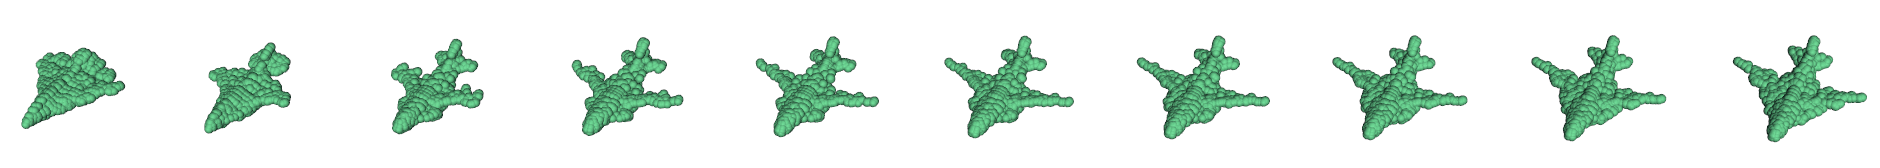
\includegraphics[width=1.0\linewidth]{PCAGAN/images/airplane_interpolation2.png}
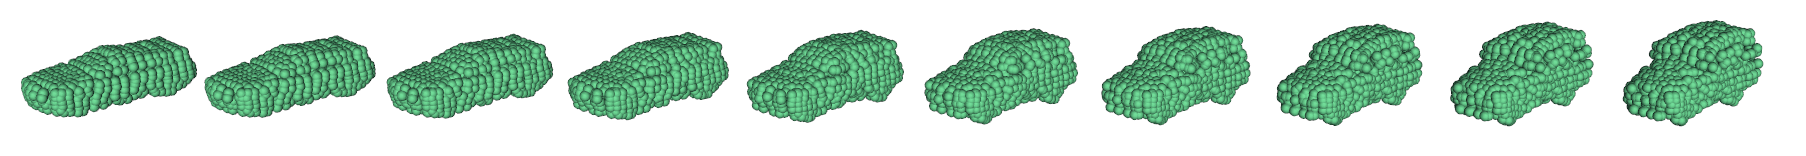
\includegraphics[width=1.0\linewidth]{PCAGAN/images/car_interpolation2.png}
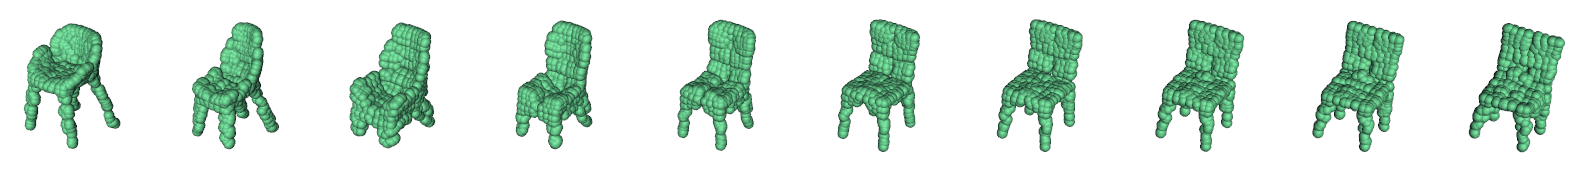
\includegraphics[width=1.0\linewidth]{PCAGAN/images/chair_interpolation2.png}
\vspace{-16pt}
\caption{\small \label{pca:interpolation} Interpolation of the encodings $z$ between a start shape and an end shape for each of the three categories shown here: airplane, car, and chair.}
\vspace{-12pt}
\end{figure}




\chapter{Multiresolution Tree Networks for 3D Point Cloud Processing}

\section{Introduction}
One of the challenges in 3D shape processing concerns the question of representation.
Shapes are typically represented as triangle meshes or point clouds in computer graphics applications due to their simplicity and light-weight nature.
At the same time an increasing number of robotic and remote-sensing applications are deploying sensors that directly collect point-cloud representations of the environment. Hence architectures that efficiently operate on point clouds are becoming increasingly desirable.

On the other hand the vast majority of computer vision techniques rely on grid-based representation of 3D shapes for analyzing and generating them. 
These include multiview representations that render a shape from a collection of views~\cite{qi2016volumetric,mvcnn,Soltani17} or voxel-based representations~\cite{wu20153d,Huang:PCL,voxnet,BrockLRW16,3dgan} that discretize point occupancy onto a 3D grid. 
Such representations allow the use of convolution and pooling operations for efficient processing. 
However, voxel-representations scale poorly with resolution and are inefficient for modeling surface details.
Even multiscale or sparse variants~\cite{fpnn,Riegler2017CVPR,hie3dcnn} incur relatively high processing cost.
Image-based representations, while more efficient, are not effective at modeling shapes with concave or filled interiors due to self occlusions.
Moreover, generating shapes as a collection of views requires subsequent reasoning about geometric consistency to infer the 3D shape, which can be challenging.


The main contribution of our work is a multiresolution tree network capable of both recognizing and generating 3D shapes directly as point clouds.
An overview of the network and how it can be applied to different applications are shown in Figure~\ref{fig:multires-abs}.
Our approach represents a 3D shape as a set of locality-preserving 1D ordered list of points at multiple resolution levels. 
We can obtain such a ordering by using space-partitioning trees such as kd-tree or rp-tree.
Feed-forward processing on the underlying tree can be implemented as 1D convolutions and pooling on the list.
However, as our experiments show, processing the list alone is not sufficient since the 1D ordering distorts the underlying 3D structure of the shape. 
To ameliorate this problem we employ a multi-grid network architecture~\cite{multigrid} where the representation at a particular resolution influences feed-forward processing at adjacent resolutions.
This preserves the locality of point in the underlying 3D shape, improves information flow across scales, enables the network to learn a coarse-to-fine representation, and results in faster convergence during training.
Our network outperforms existing point-based networks~\cite{pointnet,Klokov_2017_ICCV,pointnet2} that operate on position ($xyz$) information of points. Specifically, it obtains \textbf{91.7\%} accuracy on the ModelNet40 classification task,
while remaining efficient.
It also outperforms similar graph networks that do not maintain multiresolution representations.

Our multiresolution decoders can be used for directly generating point clouds.
This allows us to incorporate order-invariant loss functions, such as Chamfer distance, over point clouds during training. 
Moreover it can can be plugged in with existing image-based encoders for image-to-shape inference tasks.
Our method is able to both preserve the overall shape structure as well as fine details. 
On the task of single-image shape inference using the ShapeNet dataset, our approach outperforms existing voxel-based~\cite{choy20163d}, view-based~\cite{lin2018learning}, and point-based~\cite{fan2016point} techniques.

Finally, the combined encoder-decoder network can be used for unsupervised learning of shape representations in a variational autoencoder (VAE) framework. The features extracted from the encoder of our VAE (trained on the unlabeled ShapeNet dataset) leads to better shape classification results (\textbf{86.4\%} accuracy on ModelNet40) compared to those extracted from other unsupervised networks~\cite{3dgan}.

\begin{figure*}[t!]
\centering
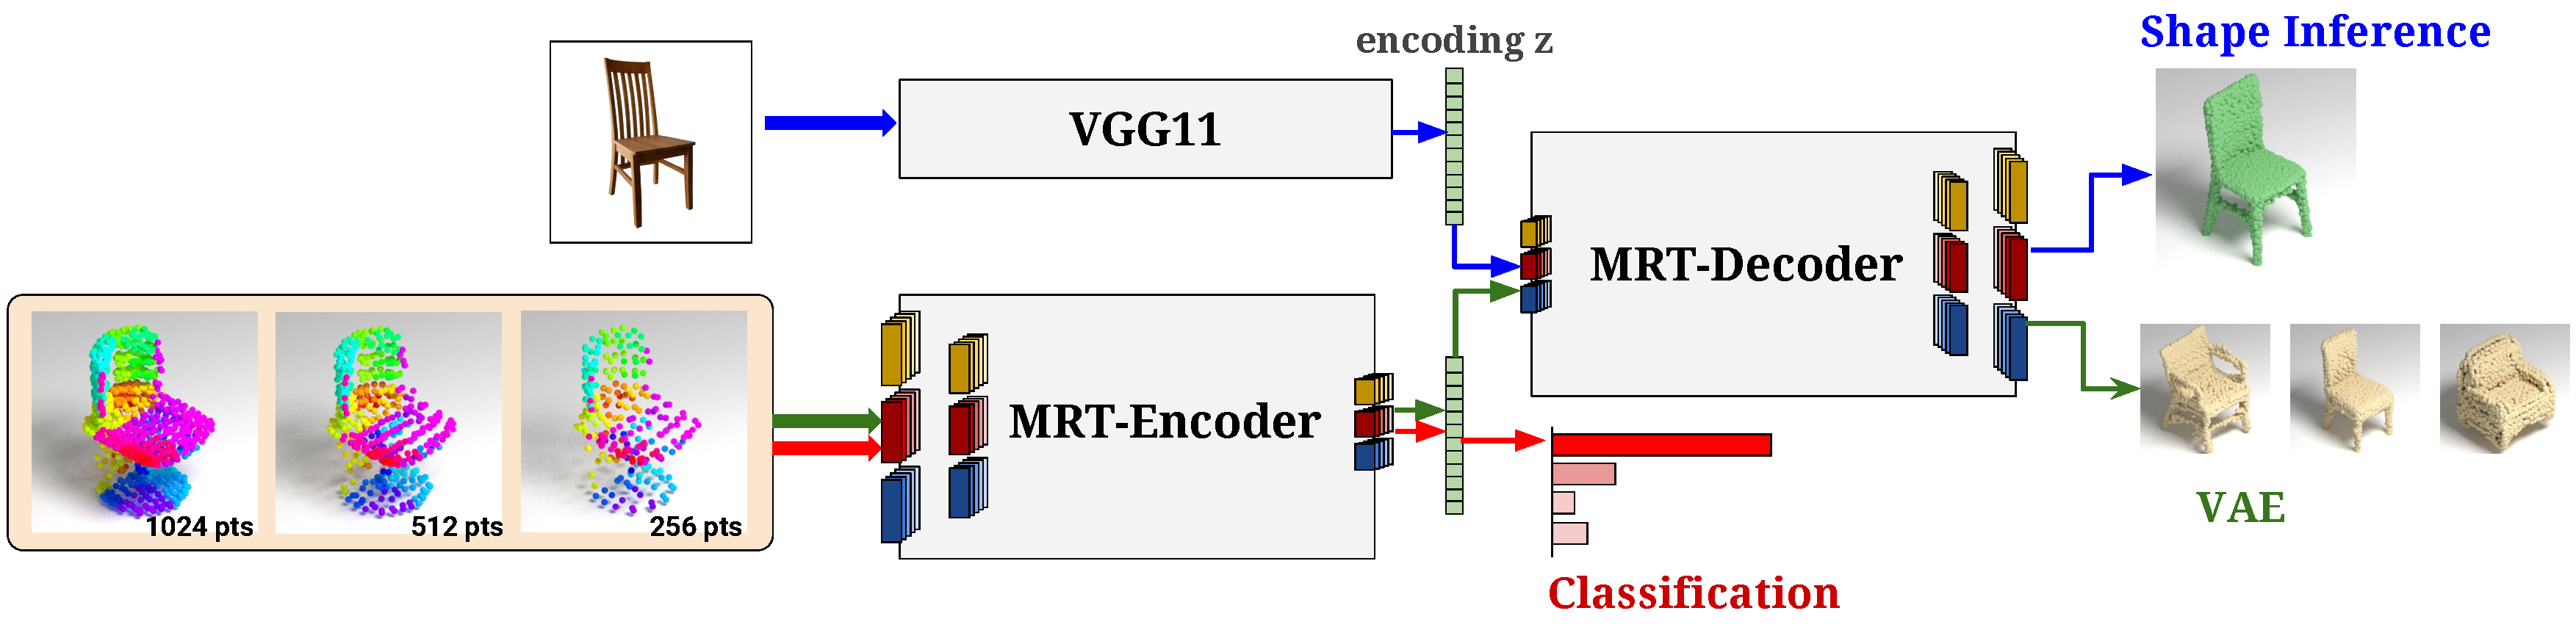
\includegraphics[width=1.0\linewidth]{imgs/visabstract1.pdf}
\vspace{-20pt}
	\caption{\small \label{fig:multires-abs}
  Overview of \mrtnet. On the left, the MRT-Encoder takes as input a 1D ordered list of points and represents it at multiple resolutions. Points are colored by their indices in the list. On the right, the MRT-Decoder directly outputs a point cloud. Our network can be used for several shape processing tasks, including classification (red), image-to-shape inference (blue), and unsupervised shape learning (green). Refer to Fig.~\ref{fig:multires-arch} for details on the encoder and decoder.}
\vspace{-16pt}
\end{figure*}






\section{Related Work}
A number of approaches have studied 3D shape recognition and generation using uniform 3D voxel grids~\cite{choy20163d,wu20153d,Huang:PCL,voxnet,BrockLRW16,3dgan}.
However, uniform grids have poor scalability and require large memory footprint, hence existing networks built upon them often operate on a relatively low-resolution grid. 
Several recent works address this issue through multiscale and sparse representations~\cite{Riegler2017CVPR,tatarchenko2017octree,ocnn,hie3dcnn,splatnet,graham17sparse} at the expense of additional book keeping. 
Still, voxel-based methods generally incur high processing cost, and are not well suited for modeling fine surface details. 
Moreover, it's not clear how to incorporate certain geometric attributes, like surface normals, into voxel representation, since these attributes do not exist in the interior of the shape.




Multiview methods~\cite{mvcnn,qi2016volumetric,Soltani17,LunGKMW17,kalogerakis20173d} represent a 3D shape as images rendered from different viewpoints. 
These methods use efficient convolutional and pooling operations and leverage deep networks pretrained on large labeled image datasets.
However, they are not optimal for general shapes with complex interior structures due to self occlusions.
Nonetheless since most models on existing shape repositories are described well by their exterior surface, view-based approaches have been adapted
for shape classification and segmentation tasks. 
Recently they have also been used for generation where a set of depth and normal maps from different viewpoints are inferred using image-based networks, and have been successfully used for image to shape generation tasks~\cite{LunGKMW17,lin2018learning}.
However such approaches requires subsequent processing to resolve view inconsistencies and outliers which is a challenging task.

Previous work has also studied extensions of ConvNets to mesh surfaces such as spectral CNNs~\cite{bruna:spectral,Yi:SyncSpec:2017}, geodesic CNNs~\cite{masci:gcnn}, or anisotropic CNNs~\cite{Boscaini2016LearningSC}. They have shown success for local correspondence and matching tasks. However, some of these methods are constrained on manifold surfaces, and generally it's unclear how well they perform on shape generation tasks.
A recent work in~\cite{SimonovskyK17} generalized the convolution operator from regular grid to arbitrary graphs while avoiding the spectral domain, allowing graphs of varying size and connectivity. 

Another branch of recent works focused on processing shapes represented as point clouds. One example is PointNet~\cite{pointnet,pointnet2}, that directly consumes point clouds as input. The main idea is to first process each point identically and independently, then leverage a symmetric function (max pooling) to aggregate information from all points. The use of max pooling preserves the permutation invariance of a point set, and the approach is quite effective for shape classification and segmentation tasks. Similarly, KD-net~\cite{Klokov_2017_ICCV} operates directly on point cloud shapes. It spatially partitions a point cloud using a kd-tree, and imposes a feed-forward network on top of the tree structure. This approach is scalable, memory efficient, achieves competitive performance on shape recognition tasks. 
While successful as encoders, it hasn't been shown how these networks can be employed as decoders for shape generation tasks.



Generating shapes as a collection of points without intermediate modeling of view-based depth maps has been relatively unexplored in the literature.
The difficulty stems from the lack of scalable approaches for generating sets.
Two recent works are in this direction.
Fan et al.~\cite{fan2016point} train a neural network to generate point clouds from a single image by minimizing Earth Mover's Distance (EMD) or Chamfer distance (CD) between the generated points and the model points. These distances are order invariant and hence can operate directly on point sets. 
This approach uses a two-branched decoder, one branch is built with 2D transposed convolutions and the other one is composed by fully connected layers.
On the other hand, our approach uses a simpler and shallower decoder built as a composition of 1D deconvolutions that operate at multiple scales.
This representation improves information flow across scales, which leads to higher quality generated shapes. 
Moreover, we use permutation invariant losses along with regularization of latent variables to build a model similar to a variational autoencoder~\cite{vae}
that can be used to sample shapes from gaussian noise.
Another work in~\cite{Gadhela:2017:3DSG} learns a distribution over shape coefficients using a learned basis for a given category using a generative adversarial network~\cite{goodfellow2014generative}. 
However, in this approach, the underlying generative model assumes a linear shape basis, which produces less detailed surfaces. 
The improved scalability of our method allows generating shapes with more points and more accurate geometric details in comparison to previous work.




Our tree network builds on the ideas of multiscale~\cite{he2014spatial,lin2016fpn}, mutligrid~\cite{multigrid} and dilated~\cite{yu2015multi} or atrous filters~\cite{dutilleux1990implementation,chen2016deeplab} effective for a number of image recognition tasks. 
They allow larger receptive fields during convolutions with a modest increase in the number of parameters.
In particular Ke et al.~\cite{multigrid} showed that communication across multiresolutions of an image throughout the network leads to improved convergence and better accuracy on a variety of tasks.
Our approach provides an efficient way of building multigrid-like representations for 3D point clouds.



\section{Method}
\label{sec:method}
\begin{figure*}
\vspace{-24pt}
\centering
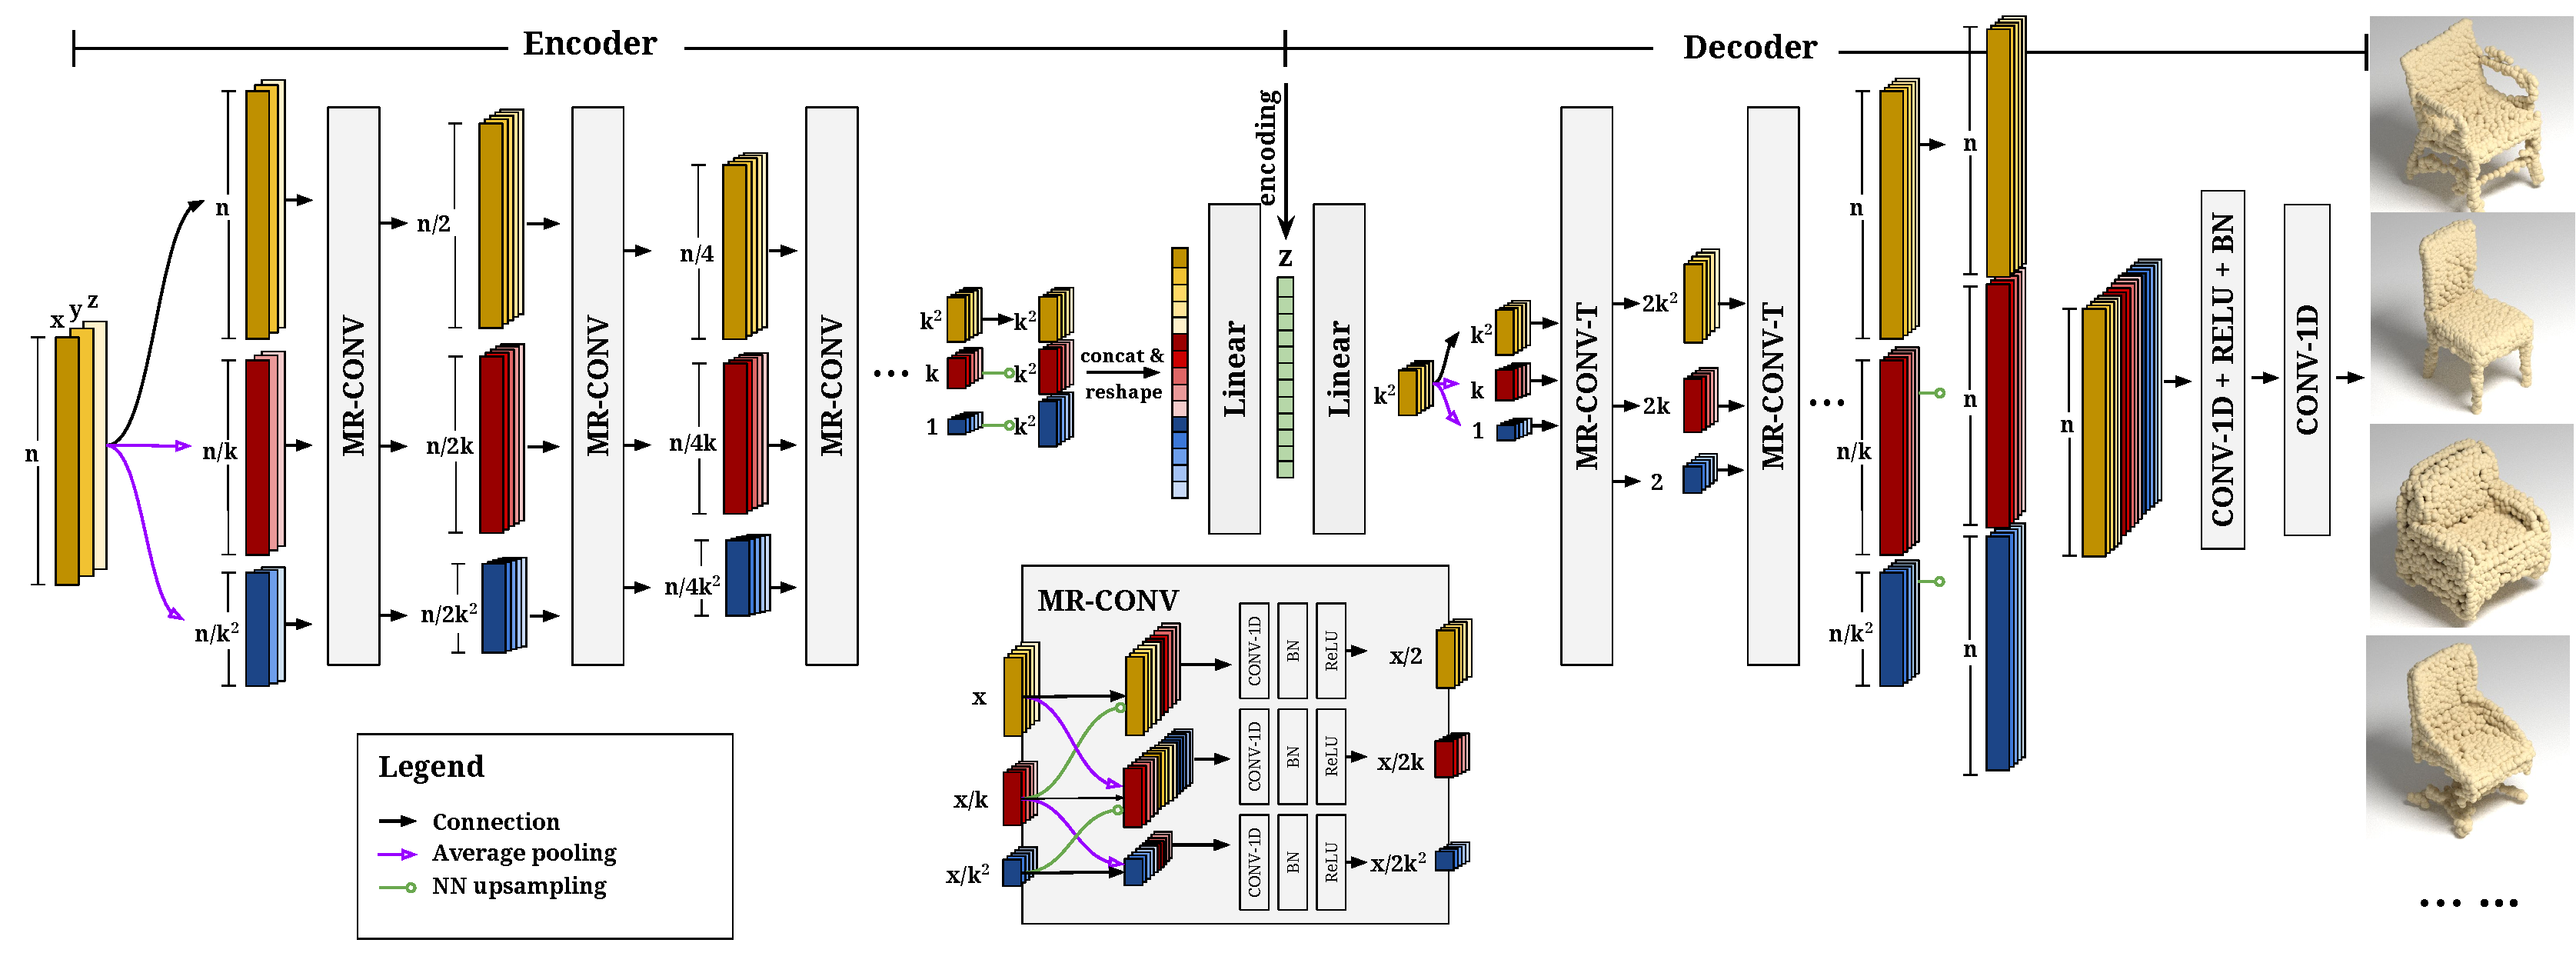
\includegraphics[width=1.0\linewidth]{MRTNet/imgs/MultiresArchitecture.pdf}
\vspace{-20pt}
	\caption{\small \label{fig:multires-arch} Our multiresolution tree network (\mrtnet) for processing 3D point clouds. We represent a 3D shape as a 1D list of spatially sorted point cloud. The network represents each layer at three scales (indicated by yellow, red, and blue), the scale ratio is $k$ between each two. The last two convolution layers have kernel size 1 and stride 1. MR-CONV refers to multi-resolution convolution (zoom-in to the inset for details); and MR-CONV-T refers to MR-CONV with transposed convolution. Our network is flexible and can be used for several shape processing tasks.}
\vspace{-16pt}
\end{figure*}
Figure~\ref{fig:multires-arch} shows the complete architecture of our multiresolution tree network (\mrtnet) that includes both the encoder and decoder.
We represent 3D shapes as a point cloud of a fixed size $\npoints=2^\depth$ (e.g. $\npoints=1K$). We center the point cloud at the origin and normalize its bounding box; then spatially sort it using a space-partitioning tree. The input to the network are thus a 1D list ($\npoints \times 3$ tensor) containing the $xyz$ coordinates of the points. The network leverages 1D convolution and represents each layer at three scales, with a ratio of $\scale$ between each two. MR-CONV refers to multi-resolution convolution, and MR-CONV-T refers to MR-CONV with transposed convolution. The encoding $\encoding$ is a 512-D vector. 
Our network architecture is flexible and can be used for several shape processing tasks. For shape \textbf{classification}, 
we use only the multiresolution encoder but adding a fully connected layer after the encoding $\encoding$ to output a 40-D vector representing the ModelNet40 shape classes. 
For \textbf{single-image shape inference}, we employ a pretrained VGG-11 image encoder~\cite{vgg}, 
combined with our multiresolution decoder to directly an output point cloud shape as a $\npoints \times 3$ tensor. 
For \textbf{unsupervised learning of point clouds}, we use both the multiresolution encoder and decoder, forming a variational autoencoder. 


\para{Spatial sorting.} As a point cloud is unordered to begin with, we use a space-partitioning tree such as KD-tree to order the points. To start, we sort the entire point set along the $x$-axis, then split it in half, resulting in equal-sized left and right subsets; we then recursively split each subset, this time along the $y$-axis; then along $z$-axis; then back along the $x$-axis and so on. Basically it's a recursive process to build a full tree where the splitting axes alternate between $x$, $y$, $z$ at each level of the tree. The order of leaf nodes naturally becomes the order of the points. There are several variants on the splitting strategy. If at each split we choose an axis among $x$, $y$, $z$ with probability proportional to the span of the subset along that axis, it builds a probabilistic KD-tree as described in~\cite{Klokov_2017_ICCV}. If we choose axes from a random set of directions, it builds an RP-tree~\cite{Dasgupta:2008:RPT}.
Note that after the ordering is obtained, the underlying details of the how the splits were taken are discarded.
This is fundamentally different from~\cite{Klokov_2017_ICCV} where the network computations are conditioned on the splitting directions.



The purpose of spatial sorting is to build a hierarchical and locality-preserving order of the points.
Thus functions computed based on the local 3D neighborhood at a point can be approximated using convolutions and pooling operations on the 1D structure.
However, any ordering of points is distortion inducing and in particular long-range relationships are not preserved well.
Maintaining multiple resolutions of the data allows us to preserve locality at different scales.
Since the partitioning is constructed hierarchically this can be efficiently implemented using pooling operations described next.






\para{Multiresolution convolution.} With the spatially sorted point set, we can build a network using 1D convolution and pooling operations. The convolution leverages the spatial locality of points after sorting, and the pooling leverages the intrinsic binary tree structure of the points. %



With a conventional CNN, each convolutional operation has a restricted receptive field and is not able to leverage both global and local information effectively. We resolve this issue by maintaining three different resolutions of the same point cloud using a mutligrid architecture~\cite{multigrid}. Different resolutions are computed directly through pooling and upsampling operations. Specifically, we use average pooling with kernel size and stride of $k$, where $k$ is a power of 2. This configuration allows pooling/downsampling the point cloud while preserving its hierarchical tree structure. Figure~\ref{fig:multires-abs} (left) shows an example point cloud at three different resolutions computed by pooling with $k=2$. For upsampling, we use nearest neighbor (NN) upsampling with a factor of $k$.

Once we can pool and upsample the point clouds, we are able to combine global and local information
in the convolutional operations by using the MR-CONV block in the inset of Fig.~\ref{fig:multires-arch}.
The multiresolution block operates in the following way.
We maintain the point cloud representations at three resolutions $\mathbf{f}_{(0)}$, $\mathbf{f}_{(1)}$, $\mathbf{f}_{(2)}$,
where the scale ratio between each two is (as mentioned above) $k$.
The MR-CONV block receives all three as input, and each resolution will be upsampled and/or pooled and concatenated with each other, creating three new representations 
$\mathbf{f}^\prime_{(0)}$, $\mathbf{f}^\prime_{(1)}$, $\mathbf{f}^\prime_{(2)}$:
\begin{equation}
\mathbf{f}^\prime_{(0)} = \mathbf{f}_{(0)} \oplus up(\mathbf{f}_{(1)}); \quad \mathbf{f}^\prime_{(1)} = pool(\mathbf{f}_{(0)}) \oplus \mathbf{f}_{(1)} \oplus up(\mathbf{f}_{(2)}); \quad \mathbf{f}^\prime_{(2)} = pool(\mathbf{f}_{(1)}) \oplus \mathbf{f}_{(2)}. \nonumber
\end{equation}
where $\oplus$ is the concatenation operation, $up$ and $pool$ are the upsampling
and average pooling operations.
Each new representation $\mathbf{f}^\prime$ then goes through a sequence of operations: 1D convolution (kernel size=2 and stride=2), batch normalization and ReLU activation.
Note that due to the stride 2, each output is half the size of its associated input.
In our generative model and shape inference model we use $k=4$, while for classification we use $k=8$.

\para{Shape classification model.} For classification, we use our multiresolution encoder in Figure~\ref{fig:multires-arch}, and add a fully connected layer after encoding $\mathbf{z}$ that outputs a 40-D vector representing the ModelNet40 classification. Specifically, we train the network on the ModelNet40~\cite{wu20153d} dataset, which contains 12,311 objects covering 40 different categories. It is split into 9,843 shapes for training and 2,468 shapes for testing. For each object, we sample 1K points on the surface using Poisson Disk sampling~\cite{Bowers:2010:PPD} to evenly disperse the points. Each sampled point cloud is then spatially sorted using the probabilistic kd-tree~\cite{Klokov_2017_ICCV}. Specifically, at each split of the tree we choose a random split axis according to the following PDF:
\begin{equation}
	P(\mathbf{n}=\mathbf{e}_i | \mathbf{x}) = \frac{\exp\{span_i(\mathbf{x})\}}{\sum_{j=1}^{d}\exp\{span_j(\mathbf{x})\}} \nonumber
\end{equation}
where $\mathbf{x}$ is the subset of points to be split, $\mathbf{n}$ is the split axis chosen from the canonical axes $\mathbf{e}_i$ (i.e. $x$,$y$,$z$ in 3D), and $span_i(\mathbf{x})$ returns the span of $\mathbf{x}$ along each axis $\mathbf{e}_i$.

The network parameters are as follows: the first MR-CONV layer has 16 filters and the following layers double the amount of filter of the previous one, unless the previous layer has 1024 filters. In that case, the next layer also has 1024 filters. The network is trained by minimizing a cross-entropy loss using an Adam optimizer with learning rate $10^{-3}$ and $\beta = 0.9$. The learning rate is decayed by dividing it by 2 every 5 training epochs. We employ scale augmentation at training and test time by applying anisotropic scaling factors drawn from $\mathcal{N}(1, 0.25)$.
At test time, for each point cloud we apply the sampled scale factors and build the probabilistic kd-tree 16 times as described above, thus obtaining 16 different versions and orderings of the point set.
Our final classification is the mean output of those versions. The test-time average has very little impact on the computation time (a discussion is included in Sec.~\ref{sec:discussions}). 


\para{Single-image shape inference.} Our multiresolution decoder can be used to perform image-to-shape inference. 
Specifically, we use a pretrained VGG-11 image encoder~\cite{vgg} combined with our decoder in Figure~\ref{fig:multires-arch}. 
Our decoder is set to generates 4K points. 
The entire network is trained using the dataset and splits provided by~\cite{choy20163d}, 
which contains 24 renderings from different views for 43783 shapes from ShapeNet divided in 13 different categories. 
We sample each ShapeNet mesh at 4K points and use them for supervision.
Given a rendered image, the task is to predict the complete point cloud (4K points) representing the object in the image.
The decoder in Figure~\ref{fig:multires-arch} has the following number of filters per layer:
512-512-256-256-128-64-64-64. As in Figure~\ref{fig:multires-arch}, the two additional
convolutional layers at the end have kernel size 1 and stride 1: the first one has 128 filters and the second one outputs the final 4K point set.

There are many possible choices for the reconstruction loss function. One straightforward choice would be to use the ordering induced by the spatial partitioning and compute the $L_2$ loss between the output and ground-truth point clouds. However, $L_2$ loss turns out to work very poorly. 
We chose to use the Chamfer distance between two point clouds ($\mathbf{x}$ and $\mathbf{y}$), defined as:
\begin{equation}
	Ch(\mathbf{x}, \mathbf{y})=
		 \frac{1}{|\mathbf{x}|}\sum_{x \in \mathbf{x}} \min_{y \in \mathbf{y}} \norm{x-y}_2 +
		 \frac{1}{|\mathbf{y}|}\sum_{y \in \mathbf{y}} \min_{x \in \mathbf{x}} \norm{x-y}_2 \nonumber
\end{equation}
The Chamfer distance is invariant to permutations of points, making it suitable to measure dissimilarities between unstructured point clouds.
The model is trained using an Adam optimizer with learning rate $10^{-3}$ and $\beta = 0.9$.
Learning rate is divided by two at each two epochs.

\para{Unsupervised learning of point clouds.} By combining the multiresolution encoder and decoder together, we can perform unsupervised learning of 3D shapes. The entire network, called \mrvae, builds upon a variational autoencoder (VAE) \cite{vae} framework. %
The encoder $Q$ receives as an input a point cloud $\mathbf{x}$ and outputs an encoding $\mathbf{z} \in \mathbb{R}^{512}$. The decoder $D$ tries to replicate the point cloud $\mathbf{x}$ from $\mathbf{z}$. Both encoder and decoder are built using a sequence of MR-CONV blocks as in Fig.~\ref{fig:multires-arch}. Similar to above, we use Chamfer distance as the reconstruction loss function. Besides this, we also need a regularization term that forces the distribution
of the encoding $\mathbf{z}$ to be as close as possible to the Gaussian $\mathcal{N}(0,I)$. Differently from the original VAE model, we found that we can get more stable training if we try to match the first two moments (mean and variance) of $\mathbf{z}$ to $\mathcal{N}(0,I)$. Mathematically, this regularization term is defined as:
\begin{equation}
	\mathcal{L}_{reg} = \norm{cov(Q(\mathbf{x}) + \delta) - I}_2 + E[Q(\mathbf{x}) + \delta] \nonumber
\end{equation}
where $cov$ is the covariance matrix, $Q$ is the encoder, $\norm{\cdot}_2$ is the Frobenius norm and $E[\cdot]$ is the
expected value.
$\delta$ is a random value sampled from $\mathcal{N}(0,cI)$ and $c=0.01$.
Thus, our generative model is trained by minimizing the following loss function:
\begin{equation}
	\mathcal{L} = Ch(\mathbf{x}, D(Q(\mathbf{x}))) + \lambda L_{reg} \nonumber
\end{equation}
We set $\lambda=0.1$. The model is trained using an Adam optimizer with learning rate $10^{-4}$ and $\beta = 0.9$.
The encoder follows the classification model and the decoder follows the one used in the shape inference model, both described previously.

\para{Shape part segmentation.} \mrtnet can also be applied for shape part segmentation tasks. For details please refer to the supplemental material.

\section{Experimental Results and Discussions}
This section presents experimental results. We implemented \mrtnet using PyTorch. 

\subsection{Shape classification} To demonstrate the effectiveness of the multiresolution encoder, we trained a baseline model that follows the same classification model but replacing multiresolution convolutions with single-scale 1D convolutions. Also, we apply the same test-time data augmentation and compute the test-time average as described in the Section~\ref{sec:method}. %

\begin{table}[t]
    \begin{minipage}{0.5\linewidth}    
    \centering
    \begin{tabular}{p{4cm}>{\centering\arraybackslash}p{1.2cm}}
        \toprule
        Method & Accuracy\\
        \midrule
        \multicolumn{2}{l}{\textit{View-based methods}}  \\
        MVCNN~\cite{mvcnn}              &  90.1   \\
        MVCNN-MultiRes~\cite{qi2016volumetric}     &  91.4    \\
        \midrule
        \multicolumn{2}{l}{\textit{Point-based methods (w/o normals)}}   \\
        KDNet (1K pts)~\cite{Klokov_2017_ICCV}  & 90.6 \\
        PointNet (1K pts)~\cite{pointnet}   & 89.2 \\
        PointNet++ (1K pts)~\cite{pointnet2} &  90.7 \\
        MRTNet (1K pts)  & \textbf{91.2} \\
        MRTNet (4K pts)& \textbf{91.7} \\
        KDNet (32K pts)~\cite{Klokov_2017_ICCV}     & \textbf{91.8} \\
        \midrule
        \multicolumn{2}{l}{\textit{Point-based methods (with normals)}}   \\
        PointNet++ (5K pts)~\cite{pointnet2} &  91.9\\
        \midrule
        \multicolumn{2}{l}{\textit{Voxel-based methods}}   \\
        OctNet~\cite{Riegler2017CVPR}       & 86.5 \\
        O-CNN~\cite{ocnn}   & 90.6\\
        \midrule
   \end{tabular}
   \caption*{\small (a) \textbf{Comparisons with previous work}. Among point-based methods that use $xyz$ data only, ours is the best in the 1K points group; and our 4K result is comparable with KDNet at 32K points.}
   \end{minipage}
   \begin{minipage}{0.5\linewidth}
   \centering
    \begin{tabular}{p{4.0cm}>{\centering\arraybackslash}p{1.2cm}}
        \toprule
        Method & Accuracy\\
        \midrule
        Full model (MRTNet, 4K pts) & 91.7 \\
        Filters/4 & 91.7 \\
        Single res. & 89.3 \\
        Single res., no aug. (kd-tree) & 86.2 \\
        Single res., no aug. (rp-tree) & 87.4\\
        \midrule
        \end{tabular}
        \caption*{\small (b) \textbf{\mrtnet ablation studies}. Filters/4 reduces the number of filters in each layer by 4. The last three rows are the single resolution model.}

    \begin{tabular}{p{4.0cm}>{\centering\arraybackslash}p{1.2cm}}
        \midrule
        Method & Accuracy\\
        \midrule
        SPH~\cite{Kazhdan:2003} & 68.2 \\
        LFD~\cite{Chen03} & 75.5 \\
        T-L Network\cite{Girdhar16} & 74.4 \\
        VConv-DAE \cite{Sharma2016} & 75.5 \\
        3D-GAN~\cite{3dgan} & 83.3 \\
        MRTNet-VAE (Ours) & \textbf{86.4} \\
        \midrule
        \caption*{\small (c) \textbf{Unsupervised representation learning}. Section~\ref{sec:exp_gen}.}
        \end{tabular}
   \end{minipage}
    \caption{Instance classification accuracy on the ModelNet40 dataset.} \label{tab:class}
    \vspace{-18pt}
\end{table}

Classification benchmark results are in Table~\ref{tab:class}(a). 
As shown in the table, \mrtnet achieves the best results among all \textbf{point-based} methods that use $xyz$ data only. In particular, ours is the best in the 1K points group. We also experimented with sampling shapes using 4K points, and the result is comparable with KDNet at 32K points -- in this case, KDNet uses 8$\times$ more points (hence 8$\times$ more memory) than ours, and is only $0.1\%$ better. PointNet++~\cite{pointnet2} with 5K points and normals is $0.2\%$ better than ours.

\setlength{\intextsep}{0pt}%
\setlength{\columnsep}{0pt}%
\begin{wrapfigure}{r}{0.35\linewidth} 
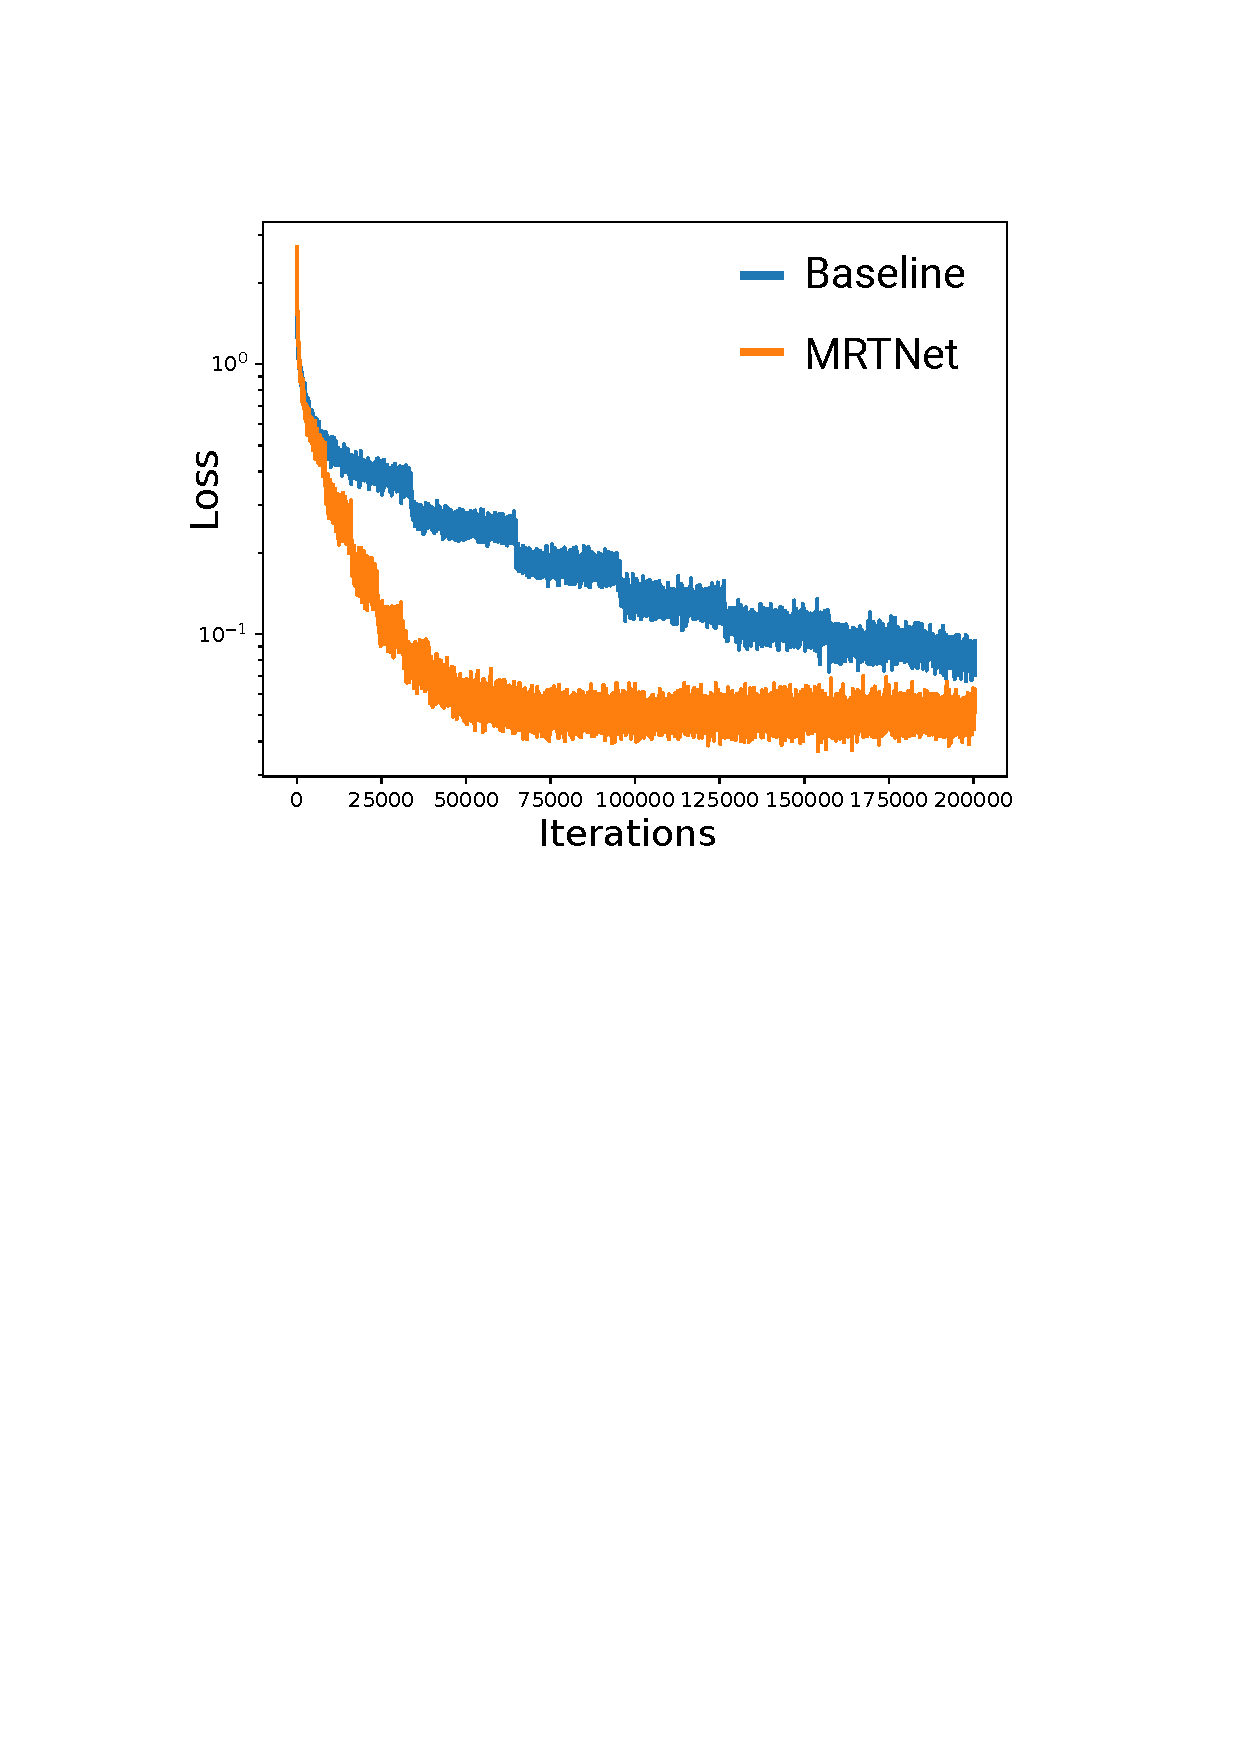
\includegraphics[width=1.0\linewidth]{imgs/convergence_loss.pdf}
\vspace{-20pt}
\caption{\small Cross entropy decay \label{fig:convergence}}
\end{wrapfigure} 
Table~\ref{tab:class}(b) shows ablation study results with variants of our approach.
Particularly, the multiresolution version is more than $2\%$ better than the baseline model (i.e. single resolution), 
while using the same number of parameters (the Filters/4 version). 
Besides, \mrtnet converges must faster than the baseline model, as we can see in the cross entropy loss decay plots in Figure~\ref{fig:convergence}. 
This shows that the multiresolution architecture leads to higher quality/accuracy and is memory efficient. 

Our single resolution baseline is akin to KDNet except it doesn't condition the convolutions on the splitting axes.
It results in $1.3\%$ less classification accuracy compared to KDNet (1K pts). This suggests that conditioning on the splitting axes during convolutions improves the accuracy.
However, this comes at the cost of extra book keeping and at least three times more parameters.
\mrtnet achieves greater benefits with lesser overhead.
Similar to the KDNet, our methods also benefit from data augmentation and can be used with both kd-trees and rp-trees.






\begin{table}[t]
\small
\centering
\begin{tabular}{c||c|c|c|c|c|c}
\hline
\multicolumn{1}{c||}{\multirow{2}{*}{\bf Category}} & \multicolumn{3}{c|}{3D-R2N2~\cite{choy20163d}} & Fan et al.~\cite{fan2016point} & Lin et al.~\cite{lin2018learning} & \mrtnet \\
& 1 view    & 3 views & 5 views & (1 view) & (1 view) & (1 view) \\ \hline
airplane & 3.207 / 2.879 & 2.521 / 2.468 & 2.399 / 2.391 & 1.301 / 1.488 & 1.294 / 1.541 & {\bf 0.976} / {\bf 0.920}\\
bench & 3.350 / 3.697 & 2.465 / 2.746 & 2.323 / 2.603 & 1.814 / 1.983 & 1.757 / 1.487 & {\bf 1.438} / {\bf 1.326}\\
cabinet & 1.636 / 2.817 & 1.445 / 2.626 & {\bf 1.420} / 2.619 & 2.463 / 2.444 & 1.814 / {\bf 1.072} & 1.774 / 1.602\\
car & 1.808 / 3.238 & 1.685 / 3.151 & 1.664 / 3.146 & 1.800 / 2.053 & 1.446 / {\bf 1.061} & {\bf 1.395} / 1.303\\
chair & 2.759 / 4.207 & 1.960 / 3.238 & 1.854 / 3.080 & 1.887 / 2.355 & 1.886 / 2.041 & {\bf 1.650} / {\bf 1.603}\\
display & 3.235 / 4.283 & 2.262 / 3.151 & 2.088 / 2.953 & 1.919 / 2.334 & 2.142 / {\bf 1.440} & {\bf 1.815} / 1.901\\
lamp & 8.400 / 9.722 & 6.001 / 7.755 & 5.698 / 7.331 & 2.347 / 2.212 & 2.635 / 4.459 & {\bf 1.944} / {\bf 2.089}\\
speaker & 2.652 / 4.335 & 2.577 / 4.302 & 2.487 / 4.203 & 3.215 / 2.788 & 2.371 / {\bf 1.706} & {\bf 2.165} / 2.121\\
rifle & 4.798 / 2.996 & 4.307 / 2.546 & 4.193 / 2.447 & 1.316 / 1.358 & 1.289 / 1.510 & {\bf 1.029} / {\bf 1.028}\\
sofa & 2.725 / 3.628 & 2.371 / 3.252 & 2.306 / 3.196 & 2.592 / 2.784 & 1.917 / {\bf 1.423} & {\bf 1.768} / 1.756\\
table & 3.118 / 4.208 & 2.268 / 3.277 & 2.128 / 3.134 & 1.874 / 2.229 & 1.689 / 1.620 & {\bf 1.570} / {\bf 1.405}\\
telephone & 2.202 / 3.314 & 1.969 / 2.834 & 1.874 / 2.734 & 1.516 / 1.989 & 1.939 / {\bf 1.198} & {\bf 1.346} / 1.332\\
watercraft & 3.592 / 4.007 & 3.299 / 3.698 & 3.210 / 3.614 & 1.715 / 1.877 & 1.813 / 1.550 & {\bf 1.394} / {\bf 1.490}\\
\hline
 \bf mean& 3.345 / 4.102 & 2.702 / 3.465 & 2.588 / 3.342 & 1.982 / 2.146 & 1.846 / 1.701 & {\bf 1.559} / {\bf 1.529}\\
\hline
\end{tabular}
\caption{\label{table:multi} \small \textbf{Single-image shape inference results}. The training data consists of 13 categories of shapes provided by~\cite{choy20163d}.     The numbers shown are [pred$\to$GT / GT$\to$pred] errors, scaled by 100. The mean is computed across all 13 categories. Our \mrtnet produces 4K points for each shape.
}
\vspace{-12pt}
\end{table}

\begin{table}[t]
\centering
\begin{tabular}{|c|c|c|}
\hline
Fully Connected & Single Res. & MRTNet \\
1.824 / 2.297 & 1.708 / 1.831 & {\bf 1.559} / {\bf 1.529} \\
\hline
\end{tabular}
\caption{\small
\label{table:ablation}
\textbf{Ablation studies for the image to shape decoder.} The numbers shown are [pred$\to$GT / GT$\to$pred] errors, scaled by 100. 
The values are the mean computed across all 13 categories.}
\vspace{-24pt}
\end{table}

\subsection{Single-image shape inference} \label{sec:exp_shapeinfer} We compare our single-image shape inference results with volumetric~\cite{choy20163d}, view-based~\cite{lin2018learning} and point-based~\cite{fan2016point} approaches using the evaluation metric by~\cite{lin2018learning}. 
Given a source point cloud $\mathbf{x}$ and a target point cloud $\mathbf{y}$, we compute
the average euclidean distance from each point in $\mathbf{x}$ to its closest in $\mathbf{y}$.
We refer to this as pred$\to$GT (prediction to groundtruth) error. It indicates how dissimilar the predicted shape is from the ground-truth.
The GT$\to$pred error is computed similarly by swapping $\mathbf{x}$ and $\mathbf{y}$, and it measures coverage (i.e. how complete the ground-truth surface was covered by the prediction).
For the voxel based model~\cite{choy20163d}, we used the same procedure as~\cite{lin2018learning},
where point clouds are formed by creating one point in the center of each surface voxel.
Surface voxels are extracted by subtracting the prediction by
its eroded version and rescale them such that the tightest 3D bounding boxes of the prediction and
the ground-truth CAD models have the same volume.

\begin{figure*}[t]
\centering
\setlength{\tabcolsep}{0pt}
\begin{tabular}{ccc|ccc|ccc}
\includegraphics[width=.108\linewidth]{rendering/srfc_comparison/FCI2PC_all_vgg_True/cc25ba35b3f6e8d3d064b65ccd8977_mrt_v1.png} &
\includegraphics[width=.108\linewidth]{rendering/srfc_comparison/FCI2PC_all_vgg_True/cc2930e7ceb24691febad4f49b26ec_mrt_v1.png} &
\includegraphics[width=.108\linewidth]{rendering/srfc_comparison/FCI2PC_all_vgg_True/cc03a89a98cd2660c423490470c47d_mrt_v1.png} &
\includegraphics[width=.108\linewidth]{rendering/srfc_comparison/SRI2PC_all_vgg_True/cc25ba35b3f6e8d3d064b65ccd8977_mrt_v1.png} &
\includegraphics[width=.108\linewidth]{rendering/srfc_comparison/SRI2PC_all_vgg_True/cc2930e7ceb24691febad4f49b26ec_mrt_v1.png} &
\includegraphics[width=.108\linewidth]{rendering/srfc_comparison/SRI2PC_all_vgg_True/cc03a89a98cd2660c423490470c47d_mrt_v1.png} &
\includegraphics[width=.108\linewidth]{rendering/srfc_comparison/MRI2PC_all_vgg_True/cc25ba35b3f6e8d3d064b65ccd8977_mrt_v1.png} &
\includegraphics[width=.108\linewidth]{rendering/srfc_comparison/MRI2PC_all_vgg_True/cc2930e7ceb24691febad4f49b26ec_mrt_v1.png} &
\includegraphics[width=.108\linewidth]{rendering/srfc_comparison/MRI2PC_all_vgg_True/cc03a89a98cd2660c423490470c47d_mrt_v1.png} \\

\includegraphics[width=.108\linewidth]{rendering/srfc_comparison/FCI2PC_all_vgg_True/cc25ba35b3f6e8d3d064b65ccd8977_mrt_green_v1.png} &
\includegraphics[width=.108\linewidth]{rendering/srfc_comparison/FCI2PC_all_vgg_True/cc2930e7ceb24691febad4f49b26ec_mrt_green_v1.png} &
\includegraphics[width=.108\linewidth]{rendering/srfc_comparison/FCI2PC_all_vgg_True/cc03a89a98cd2660c423490470c47d_mrt_green_v1.png} &
\includegraphics[width=.108\linewidth]{rendering/srfc_comparison/SRI2PC_all_vgg_True/cc25ba35b3f6e8d3d064b65ccd8977_mrt_green_v1.png} &
\includegraphics[width=.108\linewidth]{rendering/srfc_comparison/SRI2PC_all_vgg_True/cc2930e7ceb24691febad4f49b26ec_mrt_green_v1.png} &
\includegraphics[width=.108\linewidth]{rendering/srfc_comparison/SRI2PC_all_vgg_True/cc03a89a98cd2660c423490470c47d_mrt_green_v1.png} &
\includegraphics[width=.108\linewidth]{rendering/srfc_comparison/MRI2PC_all_vgg_True/cc25ba35b3f6e8d3d064b65ccd8977_mrt_green_v1.png} &
\includegraphics[width=.108\linewidth]{rendering/srfc_comparison/MRI2PC_all_vgg_True/cc2930e7ceb24691febad4f49b26ec_mrt_green_v1.png} &
\includegraphics[width=.108\linewidth]{rendering/srfc_comparison/MRI2PC_all_vgg_True/cc03a89a98cd2660c423490470c47d_mrt_green_v1.png}
\end{tabular}
\vspace{-8pt}
    \caption{\label{fig:ablation-comp} 
    \small Shapes generated by 1) the fully connected baseline; 2) the single-resolution baseline; and 3) \mrtnet.
    Colors in the first row indicate the index of a point in the output point list.}
\vspace{-6pt}
\end{figure*}

\begin{figure*}[t]
\centering
\setlength{\tabcolsep}{0pt}
\begin{tabular}{c|cccccccc}
{\rotatebox[origin=lt]{90}{Input}} &
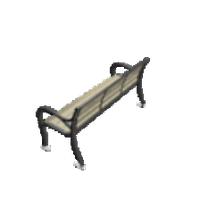
\includegraphics[width=.12\linewidth]{rendering/i2pc_comparison/c83b3192c338527a2056b4bd5d870b_alpha.png} &
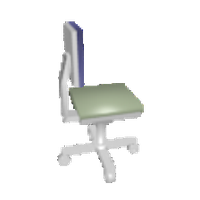
\includegraphics[width=.12\linewidth]{rendering/i2pc_comparison/cbe006da89cca7ffd6bab114dd47e3_alpha.png} &
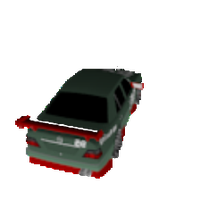
\includegraphics[width=.12\linewidth]{rendering/i2pc_comparison/cd24768b45ef5efcb1bb46d2556ba6_alpha.png} &
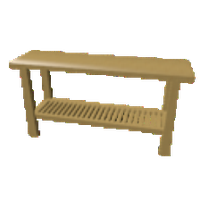
\includegraphics[width=.12\linewidth]{rendering/i2pc_comparison/cdee5ccae3613c507e1dc03b595bd3_alpha.png} &
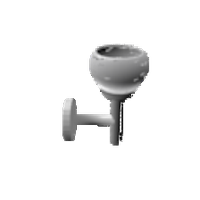
\includegraphics[width=.12\linewidth]{rendering/i2pc_comparison/d2d645ce6ad43434d42b9650f19dd4_alpha.png} &
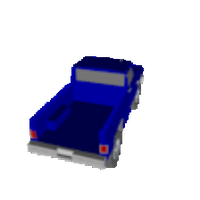
\includegraphics[width=.12\linewidth]{rendering/i2pc_comparison/ccc6b5ace9f5164d26068f53fe0ecf_alpha.png} &
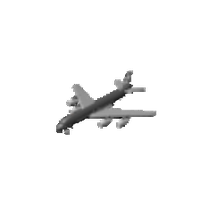
\includegraphics[width=.12\linewidth]{rendering/i2pc_comparison/d18592d9615b01bbbc0909d98a1ff2_alpha.png} &
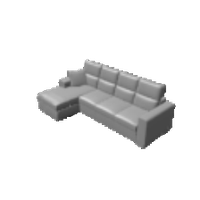
\includegraphics[width=.12\linewidth]{rendering/i2pc_comparison/cceaeed0d8cf5bdbca68d7e2f215cb_alpha.png} \\
\hline
{\rotatebox[origin=lt]{90}{G.T.}} &
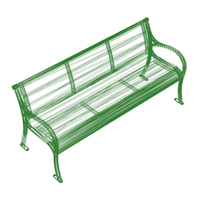
\includegraphics[width=.12\linewidth]{rendering/i2pc_comparison/gt/img1.png} &
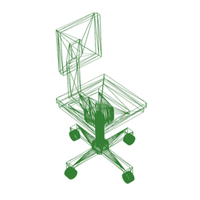
\includegraphics[width=.12\linewidth]{rendering/i2pc_comparison/gt/img2.png} &
\includegraphics[width=.12\linewidth]{rendering/i2pc_comparison/gt/img3.png} &
\includegraphics[width=.12\linewidth]{rendering/i2pc_comparison/gt/img4.png} &
\includegraphics[width=.12\linewidth]{rendering/i2pc_comparison/gt/img5.png} &
\includegraphics[width=.12\linewidth]{rendering/i2pc_comparison/gt/img6_alt.png} &
\includegraphics[width=.12\linewidth]{rendering/i2pc_comparison/gt/img7.png} &
\includegraphics[width=.12\linewidth]{rendering/i2pc_comparison/gt/img8.png} \\
\hline
{\rotatebox[origin=lt]{90}{\mrtnet}} &
\includegraphics[width=.12\linewidth]{rendering/i2pc_comparison/c83b3192c338527a2056b4bd5d870b_mrt_v1.png} &
\includegraphics[width=.12\linewidth]{rendering/i2pc_comparison/cbe006da89cca7ffd6bab114dd47e3_mrt_v1.png} &
\includegraphics[width=.12\linewidth]{rendering/i2pc_comparison/cd24768b45ef5efcb1bb46d2556ba6_mrt_v1.png} &
\includegraphics[width=.12\linewidth]{rendering/i2pc_comparison/cdee5ccae3613c507e1dc03b595bd3_mrt_v1.png} &
\includegraphics[width=.12\linewidth]{rendering/i2pc_comparison/d2d645ce6ad43434d42b9650f19dd4_mrt_v1.png} &
\includegraphics[width=.12\linewidth]{rendering/i2pc_comparison/ccc6b5ace9f5164d26068f53fe0ecf_mrt_v1.png} &
\includegraphics[width=.12\linewidth]{rendering/i2pc_comparison/d18592d9615b01bbbc0909d98a1ff2_mrt_v1.png} &
\includegraphics[width=.12\linewidth]{rendering/i2pc_comparison/cceaeed0d8cf5bdbca68d7e2f215cb_mrt_v1.png} \\
\hline
{\rotatebox[origin=lt]{90}{\small Fan~\cite{fan2016point}}} &
\includegraphics[width=.12\linewidth]{rendering/i2pc_comparison/c83b3192c338527a2056b4bd5d870b_alignedpsg_v1.png} &
\includegraphics[width=.12\linewidth]{rendering/i2pc_comparison/cbe006da89cca7ffd6bab114dd47e3_alignedpsg_v1.png} &
\includegraphics[width=.12\linewidth]{rendering/i2pc_comparison/cd24768b45ef5efcb1bb46d2556ba6_alignedpsg_v1.png} &
\includegraphics[width=.12\linewidth]{rendering/i2pc_comparison/cdee5ccae3613c507e1dc03b595bd3_alignedpsg_v1.png} &
\includegraphics[width=.12\linewidth]{rendering/i2pc_comparison/d2d645ce6ad43434d42b9650f19dd4_alignedpsg_v1.png} &
\includegraphics[width=.12\linewidth]{rendering/i2pc_comparison/ccc6b5ace9f5164d26068f53fe0ecf_alignedpsg_v1.png} &
\includegraphics[width=.12\linewidth]{rendering/i2pc_comparison/d18592d9615b01bbbc0909d98a1ff2_alignedpsg_v1.png} &
\includegraphics[width=.12\linewidth]{rendering/i2pc_comparison/cceaeed0d8cf5bdbca68d7e2f215cb_alignedpsg_v1.png} \\
\hline
{\rotatebox[origin=lt]{90}{\small Choy~\cite{choy20163d}}} &
\includegraphics[width=.12\linewidth]{rendering/i2pc_comparison/c83b3192c338527a2056b4bd5d870b_r2n2_v1.png} &
\includegraphics[width=.12\linewidth]{rendering/i2pc_comparison/cbe006da89cca7ffd6bab114dd47e3_r2n2_v1.png} &
\includegraphics[width=.12\linewidth]{rendering/i2pc_comparison/cd24768b45ef5efcb1bb46d2556ba6_r2n2_v1.png} &
\includegraphics[width=.12\linewidth]{rendering/i2pc_comparison/cdee5ccae3613c507e1dc03b595bd3_r2n2_v1.png} &
\includegraphics[width=.12\linewidth]{rendering/i2pc_comparison/d2d645ce6ad43434d42b9650f19dd4_r2n2_v1.png} &
\includegraphics[width=.12\linewidth]{rendering/i2pc_comparison/ccc6b5ace9f5164d26068f53fe0ecf_r2n2_v1.png} &
\includegraphics[width=.12\linewidth]{rendering/i2pc_comparison/d18592d9615b01bbbc0909d98a1ff2_r2n2_v1.png} &
\includegraphics[width=.12\linewidth]{rendering/i2pc_comparison/cceaeed0d8cf5bdbca68d7e2f215cb_r2n2_v1.png} \\
\hline
\end{tabular}
\vspace{-8pt}
    \caption{\label{fig:inference-comp} 
    \small Qualitative results for single-image shape inference. From top to bottom: input images, ground truth 3D shapes, results of \mrtnet, Fan et al.~\cite{fan2016point}, and Choy et al.~\cite{choy20163d}.
    }
\vspace{-12pt}
\end{figure*}

Table~\ref{table:multi} shows our results. 
Our solution outperforms competing methods in 12 out of 13 categories on the pred$\to$GT error, and in
6 categories on GT$\to$pred error.
Note that we are consistently better than the point-based methods such as~\cite{fan2016point} in both metrics; 
and we are consistently better than~\cite{lin2018learning} in the pred$\to$GT metric.
Furthermore, our method wins by a considerable margin in terms of the mean per category on both metrics. 
It is important to highlight that the multi-view based method~\cite{lin2018learning} produces tens of thousands of points and many of them
are not in the right positions, which penalizes their pred$\to$GT metric, but that helps to improve their GT$\to$pred.
Moreover, as mentioned in~\cite{lin2018learning}, their method has difficulties capturing thin structures (e.g. lamps) whereas ours is able
to capture them relatively well.
For example, our GT$\to$pred error for the \textbf{lamp} category (which contains many thin geometric structures) is more than two times smaller than the error by~\cite{lin2018learning}, indicating that MRTNet is more successful at capturing thin structures in the shapes.

\para{Ablation studies.}
In order to quantify the effectiveness of the multiresolution decoder, we compared our method with two
different baselines: a fully connected decoder and a single-resolution decoder.
The fully connected decoder consists of 3 linear layers with 4096 hidden neurons, each layer followed by batch normalization 
and ReLU activation units.
On top of that, we add a final layer that outputs $4096\times3$ values corresponding to the final point cloud, followed
by a hyperbolic tangent activation function.
The single resolution decoder follows the same architecture of the MRT decoder but replacing multiresolution convolutions with single-scale 1D convolutions.
Results are shown in Table~\ref{table:ablation}.
Note that both baselines are quite competitive. 
The single-resolution decoder is comparable to the result of~\cite{lin2018learning}, while the fully connected one achieves similar mean errors to~\cite{fan2016point}.
Still, they fall noticeably behind \mrtnet.


\begin{figure*}[t]
\centering
\setlength{\tabcolsep}{0pt}
\begin{tabular}{cccccccc}
    
\includegraphics[width=.12\linewidth]{rendering/real_MRI2PC/out_0000.png} &
\includegraphics[width=.12\linewidth]{rendering/real_MRI2PC/tables/table8_mrt.png} &
\includegraphics[width=.12\linewidth]{rendering/real_MRI2PC/out_0002.png} &
\includegraphics[width=.12\linewidth]{rendering/real_MRI2PC/tables/table2_mrt.png} &
\includegraphics[width=.12\linewidth]{rendering/real_MRI2PC/out_0004.png} &
\includegraphics[width=.12\linewidth]{rendering/real_MRI2PC/tables/table3_mrt.png} &
\includegraphics[width=.12\linewidth]{rendering/real_MRI2PC/tables/table5_mrt.png} &
\includegraphics[width=.12\linewidth]{rendering/real_MRI2PC/out_0007.png} \\

\includegraphics[width=.12\linewidth]{rendering/real_MRI2PC/out_0000_v1.png} &
\includegraphics[width=.12\linewidth]{rendering/real_MRI2PC/tables/table8_mrt_v1.png} &
\includegraphics[width=.12\linewidth]{rendering/real_MRI2PC/out_0002_v1.png} &
\includegraphics[width=.12\linewidth]{rendering/real_MRI2PC/tables/table2_mrt_v1.png} &
\includegraphics[width=.12\linewidth]{rendering/real_MRI2PC/out_0004_v1.png} &
\includegraphics[width=.12\linewidth]{rendering/real_MRI2PC/tables/table3_mrt_v1.png} &
\includegraphics[width=.12\linewidth]{rendering/real_MRI2PC/tables/table5_mrt_v1.png} &
\includegraphics[width=.12\linewidth]{rendering/real_MRI2PC/out_0007_v1.png} \\

\includegraphics[width=.12\linewidth]{rendering/real_MRI2PC/out_0000_v0.png} &
\includegraphics[width=.12\linewidth]{rendering/real_MRI2PC/tables/table8_mrt_v0.png} &
\includegraphics[width=.12\linewidth]{rendering/real_MRI2PC/out_0002_v0.png} &
\includegraphics[width=.12\linewidth]{rendering/real_MRI2PC/tables/table2_mrt_v0.png} &
\includegraphics[width=.12\linewidth]{rendering/real_MRI2PC/out_0004_v0.png} &
\includegraphics[width=.12\linewidth]{rendering/real_MRI2PC/tables/table3_mrt_v0.png} &
\includegraphics[width=.12\linewidth]{rendering/real_MRI2PC/tables/table5_mrt_v0.png} &
\includegraphics[width=.12\linewidth]{rendering/real_MRI2PC/out_0007_v0.png} \\

\hline
    
\includegraphics[width=.12\linewidth]{rendering/playdoh_shapes/plane3_mrt.png} &
\includegraphics[width=.12\linewidth]{rendering/playdoh_shapes/car8_clipped_rev_1_mrt.png} &
\includegraphics[width=.12\linewidth]{rendering/playdoh_shapes/5701697_clipped_rev_1_mrt.png} &
\includegraphics[width=.12\linewidth]{rendering/playdoh_shapes/cara_clipped_rev_1_mrt.png} &
\includegraphics[width=.12\linewidth]{rendering/playdoh_shapes/ship9_mrt.png} &
\includegraphics[width=.12\linewidth]{rendering/playdoh_shapes/ship3_mrt.png} &
\includegraphics[width=.12\linewidth]{rendering/playdoh_shapes/Play-Doh-Sofa_clipped_rev_1_mrt.png} &
\includegraphics[width=.12\linewidth]{rendering/playdoh_shapes/plane2_mrt.png} \\

\includegraphics[width=.12\linewidth]{rendering/playdoh_shapes/plane3_mrt_v0.png} &
\includegraphics[width=.12\linewidth]{rendering/playdoh_shapes/car8_clipped_rev_1_mrt_v0.png} &
\includegraphics[width=.12\linewidth]{rendering/playdoh_shapes/5701697_clipped_rev_1_mrt_v0.png} &
\includegraphics[width=.12\linewidth]{rendering/playdoh_shapes/cara_clipped_rev_1_mrt_v0.png} &
\includegraphics[width=.12\linewidth]{rendering/playdoh_shapes/ship9_mrt_v0.png} &
\includegraphics[width=.12\linewidth]{rendering/playdoh_shapes/ship3_mrt_v0.png} &
\includegraphics[width=.12\linewidth]{rendering/playdoh_shapes/Play-Doh-Sofa_clipped_rev_1_mrt_v0.png} &
\includegraphics[width=.12\linewidth]{rendering/playdoh_shapes/plane2_mrt_v0.png} \\

\includegraphics[width=.12\linewidth]{rendering/playdoh_shapes/plane3_mrt_v1.png} &
\includegraphics[width=.12\linewidth]{rendering/playdoh_shapes/car8_clipped_rev_1_mrt_v1.png} &
\includegraphics[width=.12\linewidth]{rendering/playdoh_shapes/5701697_clipped_rev_1_mrt_v1.png} &
\includegraphics[width=.12\linewidth]{rendering/playdoh_shapes/cara_clipped_rev_1_mrt_v1.png} &
\includegraphics[width=.12\linewidth]{rendering/playdoh_shapes/ship9_mrt_v1.png} &
\includegraphics[width=.12\linewidth]{rendering/playdoh_shapes/ship3_mrt_v1.png} &
\includegraphics[width=.12\linewidth]{rendering/playdoh_shapes/Play-Doh-Sofa_clipped_rev_1_mrt_v1.png} &
\includegraphics[width=.12\linewidth]{rendering/playdoh_shapes/plane2_mrt_v1.png} \\

\end{tabular}
\vspace{-8pt}
    \caption{\label{fig:real} 
    \small Shapes generated by applying \mrtnet on Inernet photos of furnitures and toys. \mrtnet is trained on the 13 categories of ShapeNet database (Table~\ref{table:multi}) . Note how the network is capable of generating detailed shapes from real photos, even though it is trained only on rendered images using simple shading models. For each output shape we show two different views.
    }
\vspace{-18pt}
\end{figure*}

In Figure~\ref{fig:ablation-comp} we visualize the structures of the output point clouds generated by the three methods.
The point clouds generated by MRTNet
present strong spatial coherence: points that are spatially nearby in 3D are also likely to be nearby in the 1D list.
This coherence is present to some degree in the single-resolution outputs (note the dark blue points in the chair's arms), but is almost completely absent in the results by the fully connected decoder. This is expected,
since fully connected layers do not leverage the spatial correlation of their inputs.
Operating at multiple scales enables MRTNet to enforce a stronger spatial coherence, allowing it to more efficiently synthesize detailed point clouds with coherent geometric structures.

\para{Qualitative results.} In Figure~\ref{fig:inference-comp} we present qualitative results of our method and comparisons to two prior works. 
The input images have 3 color channels and dimensions $224\times224$. 
In Figure~\ref{fig:real} we show results of our method applied on photographs downloaded from the Internet. 
To apply our method, we manually removed the background from the photos using~\cite{clipmagic}, which generally took less than half a minute per photo. 
As seen from the results, MRTNet is able to capture the structure and interesting geometric details of the objects (e.g. wheels of the office chairs), 
even though the input images are considerably different from the rendered ones used in training.


\begin{figure*}[t]
\centering
\setlength{\tabcolsep}{0pt}
\begin{tabular}{ccccccccc}
{\rotatebox[origin=lt]{90}{\mrtnet}} &
\includegraphics[width=.12\linewidth]{rendering/selected/mr_chairs/pc_0001.png} &
\includegraphics[width=.12\linewidth]{rendering/selected/mr_chairs/pc_0006.png} &
\includegraphics[width=.12\linewidth]{rendering/selected/mr_chairs/pc_0007.png} &
\includegraphics[width=.12\linewidth]{rendering/selected/mr_chairs/pc_0014.png} &
\includegraphics[width=.12\linewidth]{rendering/selected/mr_chairs/pc_0027.png} &
\includegraphics[width=.12\linewidth]{rendering/selected/mr_chairs/pc_0036.png} &
\includegraphics[width=.12\linewidth]{rendering/selected/mr_chairs/pc_0045.png} &
\includegraphics[width=.12\linewidth]{rendering/selected/mr_chairs/pc_0063.png} \\
{\rotatebox[origin=lt]{90}{Baseline}} &
\includegraphics[width=.12\linewidth]{rendering/selected/ae_chairs/pc_0000.png} &
\includegraphics[width=.12\linewidth]{rendering/selected/ae_chairs/pc_0001.png} &
\includegraphics[width=.12\linewidth]{rendering/selected/ae_chairs/pc_0003.png} &
\includegraphics[width=.12\linewidth]{rendering/selected/ae_chairs/pc_0004.png} &
\includegraphics[width=.12\linewidth]{rendering/selected/ae_chairs/pc_0006.png} &
\includegraphics[width=.12\linewidth]{rendering/selected/ae_chairs/pc_0007.png} &
\includegraphics[width=.12\linewidth]{rendering/selected/ae_chairs/pc_0008.png} &
\includegraphics[width=.12\linewidth]{rendering/selected/ae_chairs/pc_0009.png} \\
\end{tabular}
\vspace{-8pt}
    \caption{\label{fig:chairs-comp} 
    \small Qualitative comparisons of \mrvae with a single-resolution baseline model. Results are generated by randomly sampling the encoding $\encoding$. 
    \mrvae is able to preserve shape details much better than the baseline model, and produces less noisy outputs.}
\vspace{-6pt}
\end{figure*}
\begin{figure*}[t]
\centering
\setlength{\tabcolsep}{0pt}
\begin{tabular}{cccccccccccccccc}
\includegraphics[width=.1\linewidth]{rendering/selected/rec_shapenet/pc_0000.png} &
\includegraphics[width=.1\linewidth]{rendering/selected/rec_shapenet/pc_0002.png} &
\includegraphics[width=.1\linewidth]{rendering/selected/rec_shapenet/pc_0003.png} &
\includegraphics[width=.1\linewidth]{rendering/selected/rec_shapenet/pc_0004.png} &
\includegraphics[width=.1\linewidth]{rendering/selected/rec_shapenet/pc_0008.png} &
\includegraphics[width=.1\linewidth]{rendering/selected/rec_shapenet/pc_0011.png} &
\includegraphics[width=.1\linewidth]{rendering/selected/rec_shapenet/pc_0013.png} &
\includegraphics[width=.1\linewidth]{rendering/selected/rec_shapenet/pc_0015.png} &
\includegraphics[width=.1\linewidth]{rendering/selected/rec_shapenet/pc_0016.png} &
\includegraphics[width=.1\linewidth]{rendering/selected/rec_shapenet/pc_0018.png} \\
\includegraphics[width=.1\linewidth]{rendering/selected/rec_shapenet/pc_0025.png} &
\includegraphics[width=.1\linewidth]{rendering/selected/rec_shapenet/pc_0026.png} &
\includegraphics[width=.1\linewidth]{rendering/selected/rec_shapenet/pc_0027.png} &
\includegraphics[width=.1\linewidth]{rendering/selected/rec_shapenet/pc_0033.png} &
\includegraphics[width=.1\linewidth]{rendering/selected/rec_shapenet/pc_0035.png} &
\includegraphics[width=.1\linewidth]{rendering/selected/rec_shapenet/pc_0037.png} &
\includegraphics[width=.1\linewidth]{rendering/selected/rec_shapenet/pc_0042.png} &
\includegraphics[width=.1\linewidth]{rendering/selected/rec_shapenet/pc_0044.png} &
\includegraphics[width=.1\linewidth]{rendering/selected/rec_shapenet/pc_0048.png} &
\includegraphics[width=.1\linewidth]{rendering/selected/rec_shapenet/pc_0054.png}
\end{tabular}
\vspace{-12pt}
    \caption{\label{fig:gallery} 
    \small Test set shapes reconstructed by \mrvae trained on all categories of ShapeNet (using 80\%/20\% training/test split). \mrvae is able to reconstruct high-quality diverse shapes.}
    \vspace{-8pt}
\end{figure*}

\subsection{Unsupervised Learning of Point Clouds} \label{sec:exp_gen}
For unsupervised learning of point clouds, we train our \mrvae using the ShapeNet dataset~\cite{chang2015shapenet}. 
By default we compute $N=4K$ points for each shape using Poisson Disk sampling~\cite{Bowers:2010:PPD} to evenly disperse the points. 
Each point set is then spatially sorted using a \kdtree. 
Here we use the vanilla \kdtree where the splitting axes alternate between $x$, $y$, $z$ at each level of the tree. 
The spatially sorted points are used as input to train the \mrvae network (Section~\ref{sec:method}). 
Similar to before, we also train a baseline model that follows the same network but replacing multiresolution convolutions with single-scale 1D convolutions
in both encoder and decoder. 
As Figure~\ref{fig:chairs-comp} shows, the shapes generated by the \mrvae trained on chairs are of considerably higher quality than those generated by the baseline model. 

We also performed multiple-category shape generation by training \mrvae on $80\%$ of the objects from ShapeNet dataset. 
The remaining models belong to our test split. 
Reconstructions of objects in the test split are included in Figure~\ref{fig:gallery}. 
Even when trained with a greater variety of shapes, the \mrvae is able to reconstruct high quality shapes from its embedding. 
This demonstrates that \mrvae is suitable for various inference tasks such as shape completion or point cloud reconstructions.

\para{Point ordering in the generated shapes.} 
A useful way to analyze shape generation is to see if the generated points have any consistent ordering across different shapes. 
This is an interesting question because as described previously, our \mrvae is trained using Chamfer Distance, 
a metric that's invariant to permutations of points. 
While the input to the network is all spatially sorted, the output is not restricted to any particular order and can in theory assume any arbitrary order. 
In practice, similar to the image-to-shape model, we observe that there is a consistent ordering of points in the generated shapes, as shown in Figure~\ref{fig:corresp}. 
Specifically, we picked three index ranges from one example chair, one at the top, one on the side, and one close to the bottom, 
then we color coded points in each shape that fall into these three index ranges. 
In the figure we can see clearly that they fall into approximately corresponding regions on each chair shape.

\begin{figure*}[t]
\centering
\setlength{\tabcolsep}{0pt}
\begin{tabular}{cccccccccccc}
\includegraphics[width=.083\linewidth]{rendering/selected/corresp/m1.png} &
\includegraphics[width=.083\linewidth]{rendering/selected/corresp/m2.png} &
\includegraphics[width=.083\linewidth]{rendering/selected/corresp/m3.png} &
\includegraphics[width=.083\linewidth]{rendering/selected/corresp/m4.png} &
\includegraphics[width=.083\linewidth]{rendering/selected/corresp/m5.png} &
\includegraphics[width=.083\linewidth]{rendering/selected/corresp/m6.png} &
\includegraphics[width=.083\linewidth]{rendering/selected/corresp/m7.png} &
\includegraphics[width=.083\linewidth]{rendering/selected/corresp/m8.png} &
\includegraphics[width=.083\linewidth]{rendering/selected/corresp/m9.png} &
\includegraphics[width=.083\linewidth]{rendering/selected/corresp/m10.png} &
\includegraphics[width=.083\linewidth]{rendering/selected/corresp/m11.png} &
\includegraphics[width=.083\linewidth]{rendering/selected/corresp/m12.png} 
\end{tabular}
\vspace{-8pt}
    \caption{\small \label{fig:corresp} Point correspondences among different shapes generated by \mrvae. 
	We picked three index ranges (indicated by three colors) from one example chair, and then color coded points in every shape that fall into these three ranges. 
	The images clearly show that the network learned to generate shapes with consistent point ordering.
    }
    \vspace{-4pt}
\end{figure*}

\begin{figure*}[t]
\centering
\setlength{\tabcolsep}{0pt}
\begin{tabular}{cccccccccc}
\includegraphics[width=.1\linewidth]{rendering/selected/interp1/pc_0000.png} &
\includegraphics[width=.1\linewidth]{rendering/selected/interp1/pc_0004.png} &
\includegraphics[width=.1\linewidth]{rendering/selected/interp1/pc_0006.png} &
\includegraphics[width=.1\linewidth]{rendering/selected/interp1/pc_0008.png} &
\includegraphics[width=.1\linewidth]{rendering/selected/interp1/pc_0009.png} &
\includegraphics[width=.1\linewidth]{rendering/selected/interp1/pc_0049.png} &
\includegraphics[width=.1\linewidth]{rendering/selected/interp1/pc_0058.png} &
\includegraphics[width=.1\linewidth]{rendering/selected/interp1/pc_0070.png} &
\includegraphics[width=.1\linewidth]{rendering/selected/interp1/pc_0080.png} &
\includegraphics[width=.1\linewidth]{rendering/selected/interp1/pc_0099.png} \\
\includegraphics[width=.1\linewidth]{rendering/selected/interp2/pc_0000.png} &
\includegraphics[width=.1\linewidth]{rendering/selected/interp2/pc_0004.png} &
\includegraphics[width=.1\linewidth]{rendering/selected/interp2/pc_0007.png} &
\includegraphics[width=.1\linewidth]{rendering/selected/interp2/pc_0009.png} &
\includegraphics[width=.1\linewidth]{rendering/selected/interp2/pc_0010.png} &
\includegraphics[width=.1\linewidth]{rendering/selected/interp2/pc_0011.png} &
\includegraphics[width=.1\linewidth]{rendering/selected/interp2/pc_0012.png} &
\includegraphics[width=.1\linewidth]{rendering/selected/interp2/pc_0014.png} &
\includegraphics[width=.1\linewidth]{rendering/selected/interp2/pc_0017.png} &
\includegraphics[width=.1\linewidth]{rendering/selected/interp2/pc_0019.png} 
\end{tabular}
    \vspace{-8pt}
    \caption{\small \label{fig:interp} Shape interpolation results. For each example, we obtain the encodings $\encoding$ of the starting shape and ending shape, then linearly interpolate the encodings and use the decoder to generate output shapes from the interpolated $\encoding$. Results show plausible interpolated shapes.
    }
    \vspace{-16pt}   
\end{figure*}

\para{Shape interpolation.} Another common test is shape interpolation: pick two encodings (either randomly sampled, or generated by the encoder for two input shapes), linearly interpolate them and use the decoder to generate the output shape. 
Figure~\ref{fig:interp} shows two sets of interpolation results of chairs from the ShapeNet dataset.


\para{Unsupervised classification.} A typical way of assessing the quality of representations learned in a unsupervised setting is to use them as features for classification. 
To do so, we take the \mrvae model trained with all ShapeNet objects, and use its features to classify ModelNet40~\cite{wu20153d} objects. 
Our classifier is a single linear layer, where the input is a set of features gathered from the first three layers of the \mrvae encoder. 
The features are constructed this way: we apply a pooling operation of size 128, 64 and 32 respectively on these three layers; 
then at each layer upsample the two smaller resolutions of features to the higher resolution such that all three resolutions have the same size. 
Finally, we concatenate all those features and pass them through a linear layer to get the final classification. 
It is important to notice that we did not perform any fine-tuning: the only learned parameters are those from the single linear layer. 
We used an Adam optimizer with learning rate $10^{-3}$ and $\beta=0.9$. 
The learning rate is decayed by dividing it by 2 every 5 epochs. 
Using this approach, we obtained an accuracy of $86.34\%$ on the ModelNet40 classification benchmark, as shown in Table~\ref{tab:class}(c). 
This result is considerably higher compared to similar features extracted from unsupervised learning in other autoencoders.
This shows that the representations learned by our \mrvae is more effective at capturing and linearizing the latent space of training shapes.


\vspace{-8pt}

\subsection{Discussions} \label{sec:discussions}
\para{Robustness to transformations.} Kd-trees are naturally invariant to point jittering as long as it's small enough so as to not alter the shape topology. 
Our approach is invariant to translations and uniform scaling as the models are re-centered at the origin and resized to fit in the unit cube. On the other hand, kd-trees are not invariant to rotations. 
This can be mitigated by using practices like pooling over different rotations (e.g. MVCNN) or branches that perform pose prediction and transformation (e.g. PointNet). 
However, we notice that simply having unaligned training data was enough to account for rotations in the classification task, and the ModelNet40 dataset contains plenty of unaligned shapes. 
Moreover, since the KDNet~\cite{Klokov_2017_ICCV} also employs a kd-tree spatial data structure, the discussions there about transformations also apply to our method.

\para{Computation time.} Building a kd-tree of $N$ points takes $O(N \log N)$ time, where $N=2^{10}$ for 1K points. 
While PointNet does not require this step, it's also more than 2.0\% worse in the classification task. 
The time to run a forward pass for classification is as follows: PointNet takes 25.3ms, while MRTNet takes 8.0ms on a TITAN GTX1080, both with batch size of 8.
Kd-tree building is also much faster than rendering a shape multiple times like in MVCNN~\cite{mvcnn} or voxelizing it~\cite{Riegler2017CVPR}. 
Using 16 different test-time augmentations does not have significant impact in computational time, as the 16 versions are classified in the same batch. 
This number of test-time augmentations is comparable to other approaches, e.g. 10 in~\cite{Klokov_2017_ICCV}, 80 in~\cite{mvcnn}, and 12 in~\cite{ocnn} and~\cite{pointnet}.


\section{Conclusion}

In conclusion, we introduced multiresolution tree networks (\mrtnet) for point cloud processing. They are flexible and can be used for shape classification, generation, and inference tasks. Our key idea is to represent a shape as a set of locality-preserving 1D ordered list of points at multiple resolutions, allowing efficient 1D convolution and pooling operations. 
The representation improves information flow across scales, enabling the network to perform coarse-to-fine analysis, leading to faster convergence during training
and higher quality for shape generation. 

In future work, we would like to incorporate additional point attributes, such as normal and color, into the network, 
to further improve accuracy of shape recognition and allow the shape generator to produce these attributes. 
We would also like to apply 
and extend the method to process spatio-temporal shape analysis, such as on animated shapes or other temporarlly changing 3D point data.


\chapter{Learning Generative Models of Shape Handles}

% \nipsfinalcopy is no longer used
\begin{figure}[h!]
\centering
  %\includegraphics[width=\linewidth]{imgs/genshapes.png}
  \includegraphics[width=0.32\linewidth]{handles/imgs/airplane-montage.png}
  \includegraphics[width=0.32\linewidth]{handles/imgs/chair-montage.png}
  \includegraphics[width=0.32\linewidth]{handles/imgs/chair-montage-sm.png}
  \caption{\small\label{fig:bunny} 
  \textbf{Gallery of 3D shapes generated as sets of handles \emph{(zoom for details)}.}
  We propose a class of generative models for synthesizing sets of handles --
  lightweight proxies that can be easily utilized for high-level tasks such as shape editing, parsing, animation etc.
  Our model can generate sets with different cardinality and is flexible to work with various types of handles, such as sphere-mesh handles~\cite{spheremesh} (first and third figures) and 
  cuboids (middle figure).
  }
 \end{figure}

\section{Introduction}
\label{sec:introduction}
Dramatic improvements in quality of image generation have become a key driving force behind many novel image editing applications.
%, such as image synthesis from semantic data (\eg., pixel labels or text), inpainting and super resolution.
%Generative models for images have seen remarkable improvements in quality in recent years~\cite{progressivegan, stylegan, biggan, sngan} and
%are one of the most researched fields in deep learning.
%These models 
%have become a central component in several image editing applications, such as 
%semantic image synthesis~\cite{spade,pix2pixhd,pix2pix},
%image inpainting~\cite{deepfillv1,deepfillv2,partconv}, 
%super-resolution~\cite{srgan,esrgan} and
%text-based image generation~\cite{stackgan,attngan,zhang2018cvpr}.
Yet, similar approaches are lacking for editing and generating 3D shapes.
There are two related challenges.
%It would be certainly desirable to extend such success to 3D shapes as well. 
%Unfortunately, editing and generating 3D geometry is a significantly harder problem.
%The task is challenging for a number of reasons.
First, learning generative models for 3D data is challenging, as unlike images, high-quality 3D data is hard to obtain and the data is high dimensional and often unstructured.
%%\radomir{and in most cases what matters is the shape of the 3D surface and not what is inside or outside, which in 2D is closer to vector art than images)}, increasing the complexity of the networks. 
%Second, high-quality 3D data is harder to obtain. 
%smaller in comparison to the image counterpart, making it significantly more challenging to learn. 
Second, regardless of whether good generative models are available,
manipulating and editing 3D shapes in interactive applications is harder to users than editing images.
%still a challenging task.
%interacting with 3D shapes poses additional challenges.
%In other words, even if we are able to generate high-quality shapes, 
%manipulating and reasoning about these shapes is still a challenging task.
For this reason, the geometry processing community has developed techniques for representing
3D data as a small collection of simpler \emph{proxy shapes}~\cite{ocd, acd, meshsegprim, abstractionshapes, variationalshape, obbcage, bmesh}.
%These lightweight proxies can be used as stand-ins or \emph{handles} to the original 3D data 
%for automatic or interactive processes. %\rui{`substitutes' sounds a bit awkward as it doesn't convey that you want the proxy shapes to approximate the original 3D as close as possible} \radomir{what about: can be used to represent the original 3D data...}.
%\giorgio{then maybe connect sparsity with ease of manipulation?} \tamy{I think the sentence is fine, there is a "or", sometimes handle sets are substitutes, not for visual purpose, but for interaction or simplified simulations.} 
In this paper, we refer to these light-weight proxies as \emph{shape handles} due to their ability to be easily manipulated by users.
These representations have been widely used in tasks that require interaction and high-level
reasoning in 3D environments, such as shape editing~\cite{gsmc_iwires_sig_09, spheremesh}, 
animation~\cite{animatedsm}, grasping~\cite{graspplaning}, and tracking~\cite{smhandtrack}.

%\begin{figure}
%\centering
%\includegraphics[width=1.0\linewidth]{imgs/handles.png}
%\caption{\label{fig:handles} \small
%\textbf{Different types of handles}.
%Cuboids, cages~\cite{obbcage}, wires~\cite{gsmc_iwires_sig_09} and sphere-meshes~\cite{spheremesh} are examples of shape handles.
%They are compact shape representations that were designed to be used
%in tasks like shape editing, deformation and grasping.}
%\end{figure}


We propose a generative models of shape handles. % that address these challenges.\rui{what challenges?}
Our method adopts a two-branch network architecture to generate shapes with varying number of handles, where one branch focuses on generating handles while the other predicts the existence of each handle
(Section~\ref{sec:cardinality}). 
%Training these branches in an alternating fashion enables us to generate sets with different cardinality. 
Furthermore, we propose a novel similarity measure based on distance fields to compare shape handle pairs. 
This measure can be easily adapted to accommodate various type of handles, such as cuboids and sphere-meshes~\cite{spheremesh}
(Section~\ref{sec:similarity}). 
Finally, in contrast to previous work~\cite{Tulsiani2017, Paschalidou2019} which focuses on unsupervised methods, we leverage recent works in collecting 3D annotations~\cite{partnet} as well as shape summarization techniques~\cite{spheremesh} to provide supervision to our approach.
%We demonstrate how we can use pre-computed sets of handles as a supervisory signal through a versatile framework, adaptable to various types of handles and capable of generating sets with varying cardinality.  
%We note that 3D shapes often possess a rich variation in both number of components and overall topology which is predicted with our network structure.
%In particular, we use handles extracted from human annotations in the
%PartNet dataset and sphere-meshes on ShapeNet
%dataset.
Experiments show that our method significantly outperforms previous methods
on shape parsing and generation tasks.
Using self-supervised training data generated by~\cite{spheremesh}, our approach produces shapes that are twice as accurate as competing approaches in terms of intersection-over-union (IoU) metric. 
By employing human annotated data, our model can be further improved, achieving even higher accuracy than using self-supervised training data.
Moreover, as shape handles provide a compact representation, our generative networks are compact (less than 10MB).
Despite the small memory footprint,
our method generates a diverse set of
high quality 3D shapes, as seen in Figure~\ref{fig:bunny}.

Finally, our method is built towards generating shapes using
representations that are amenable to manipulation by users.
In contrast to point clouds and other 3D representations such as occupancy grids,
handles are intuitive to modify and naturally suitable for editing and animation tasks.
The latent space of shape handles induced by the learned generative model can be leveraged to support shape editing, completion, and interpolation tasks, as depicted in Figure~\ref{fig:handles}.

%Thus, relationships between handles that were previously defined by heuristics, like
%in~\cite{gsmc_iwires_sig_09}, can be learned directly from data.
%Additionally, such models can be combined with image encoders to reconstruct
%shapes directly as sets of handles, or coupled with point cloud or volumetric encoders
%to perform shape parsing in a single forward pass.

%Despite these benefits, few approaches have
%explored the use of shape handles as a 3D representation for generative models.
%This is not surprising: achieving such capabilities requires developing
%models that can generate sets of objects of varying cardinality. 
%While previous work has studied generative models for point clouds~\cite{}, %representing each shape as a set of 3D points, 
%such approaches generally require pre-selecting a fixed number of points. In contrast, approximating shapes as sets of handles needs to %accommodate variable sizes -- a simple shape should be described by
%a couple of handles, whereas a complex shape requires dozens of handles.
%Moreover, training a generative model for sets of handles requires
%a similarity metric that efficiently compares the individual elements. %\rui{again, I suppose you mean defining approximate similarity metric?} -- what is an efficient way
%of computing similarity between two cylinders? or two triangles? or two curves in 3D? \rui{someone could be reading this and not understanding why it's hard to compare similarity between two cynlinders?}
%Ideally, we would like this metric to be easily applicable to different type of handles as well.

%\maji{I'd move this paragraph up. The previous two paragraphs sound like related work.}
%In this paper, we propose a method to learn generative models of shape handles that can address these challenges. %Our method is %adaptable to various types of handles and capable of generating sets with varying cardinality. 
%In order to generate sets with varying number of handles, we propose a two-branch network architecture where one branch focuses on generating handles while the other predicts the existence of each handle. Training these branches in an alternating fashion enables us to generate sets with different cardinality. Furthermore, we propose a novel similarity measure based on distance fields to compare shape handle pairs. This measure can be easily adapted to various type of handles such as cuboids and \tamy{sphere-meshes}~\cite{spheremesh}. Finally, in contrast to previous work~\cite{Tulsiani2017, Paschalidou2019} which focuses on unsupervised methods, we leverage the recent efforts in 3D annotation tasks as well as the shape summarization techniques~\cite{spheremesh} developed in the graphics community to provide supervision. 
%We demonstrate how we can use pre-computed sets of handles as a supervisory signal through a versatile framework, adaptable to various types of handles and capable of generating sets with varying cardinality.  
%We note that 3D shapes often possess a rich variation in both number of components and overall topology which is predicted with our network structure.
%In particular, we experiment with handles extracted from human annotations in the
%PartNet~\cite{partnet} dataset and from sphere-meshes computed on ShapeNet~\cite{shapenet}
%shapes using~\cite{spheremesh}.
%Our experiments show that our method significantly outperforms previous techniques
%on shape parsing and generation tasks.
%Using self-supervision from~\cite{spheremesh} our approach generates shapes \textbf{63\%} more accurate in terms of %intersection-over-union (IOU)
%than other unsupervised approaches. %\rui{might want to spell out the evaluation metric upfront: is 63\% in terms of IOU or some other metric?}
%Similarly, by employing human annotations, our approach is capable of generating shape approximations 
%\textbf{two times} more precise than its unsupervised counterparts.
%Talk specifically about the results once sec 4 is complete.
\section{Related work}
\label{sec:related}

\paragraph{Deep generative models of 3D shapes.}
Multiple 3D shape representations have been used in the context of
deep generative models.
3D voxel grids~\cite{choy20163d, prgan} are a natural extension to image-based architectures,
but suffer from high memory footprint requirements.
Sparse occupancy grids~\cite{Wang-2017-ocnn, tatarchenko2017octree, hie3dcnn, matryoshka} alleviate this issue using a hierarchical grid,
but they are still not able to generate detailed shapes and they require additional bookkeeping.
Multi-view representations ~\cite{Soltani17, LunGKMW17}, point clouds~\cite{fan2016point, mrt18, pcagan, latentpc}, mesh deformations~\cite{pixel2mesh, cmrKanazawa18}
and implicit functions~\cite{park2019deepsdf, mescheder2019occupancy, chen2019learning, genova2019learning} provide alternatives that are compact and capable
of generating detailed shapes.
However, these approaches are focused on reconstructing accurate 3D shapes and
are not amenable to tasks like editing.
Our goal is different: we explore generative models to produce sets of handles --
summarized shape representations that can be easily manipulated by users.

\begin{figure}
\centering
\includegraphics[width=0.8\linewidth]{handles/imgs/pipeline.png}
\caption{\label{fig:handles}
\textbf{Overview}.
We propose a method to train a generative model $g$ for sets of shape handles.
Once trained, the latent representation $z$ can also be used in applications like
shape editing and interpolation.}
\vspace{-14pt}
\end{figure}


%Even though images require a smaller memory footprint than occupancy grids,
%they are not ideal either: as there is no explicit 3D representation, some synthesized pixels do not correspond to any surface, while others may appear in many different views but with no consensus on the corresponding 3D point, leading to a sub-optimal representation.
%Meshes and point clouds do not suffer from these limitations.
%Every generated triangle or point is, by construction, a part of the surface.
%However, meshes are notoriously hard to generate using deep neural networks.
%The techniques are usually limited to generating vertex positions in a pre-defined mesh topology~\cite{},
%or by generating meshes as a post-processing step~\cite{}.
%On the other hand, point cloud generation techniques are more flexible, capable of approximating
%shapes of arbitrary topology.
%While some methods generate 3D point clouds directly~\cite{}, others generate points via learned surface parameterizations~\cite{}.
%A key component of these approaches is the utilization of permutation invariant losses capable
%of computing similarity between sets of points.
%In this work, we extend these losses to allow comparisons between sets of primitives.
%
%Recent research focuses on representing shapes as the level sets of implicit
%functions parameterized by neural networks~\cite{}.
%This representation is capable of seamlessly representing shapes of different topologies
%with low memory footprints.
%However, implicit functions are high dimensional %and often non-parsimonious \nathan{ I am not sure this can be argued that implicit forms imply non-parsimony it depends how they are used.  } \rui{this is a well-known term?} 
%and are not naturally suitable
%for shape editing or other high-level reasoning tasks, like path planning or grasping.
%Our goal is to generate shapes represented by a small set of primitive components
%that can be easily manipulated and utilized by high-level reasoning systems.  \rui{the above two paragraphs are very long and it could be dramatically simplified, by saying that these techniques are focused on generating detailed 3D shapes but they are not naturally amenable for shape editing. Our goal is different, blah blah.}

Two closely related methods to ours are Tulsiani et al.~\cite{Tulsiani2017} and Paschalidou et al.~\cite{Paschalidou2019} where they propose models
to generate shapes as a collection of primitives \emph{without supervision}.
%The problem we tackle here is fundamentally different -- 
In contrast, we are focused
on creating models capable of utilizing shape decompositions provided by external
agents; either a human annotator or a shape summarization technique.
We demonstrate that, by using the extra information provided by annotations or well known
geometric processing techniques, our method is capable of generating
more accurate shapes while keeping the representation interpretable and intuitive for easy
editing.
Other approaches focused on learning shape structures through stronger 
supervision~\cite{li_sig17, mo2019structurenet, im2struct}, requiring not only handle description,
but also relationships between them, e.g. support, symmetry, adjacency, hierarchy, etc.
In contrast, our method models shapes as sets and we show that inter-handle relationships
can be learned directly from data, so that the latent space induced by our model can be used to guide shape editing, completion, and interpolation tasks.
Furthermore, we present a general framework that can be easily adapted to different types of handles,
not only a single parametric family, like cuboids~\cite{Tulsiani2017, mo2019structurenet, li_sig17} or superquadrics~\cite{Paschalidou2019}.

\paragraph{Methods for shape decomposition.}
Shape decomposition has been extensively studied by the geometry processing
literature. The task is to approximate a complex shape as a set of simpler, lower-dimensional
parts that are amenable for editing. We refer to these parts as \emph{shape handles}. Early cognitive studies have shown that humans tend to reason about 3D shapes as a union
of convex components~\cite{partsrecognition}. Multiple approaches have explored decomposing shapes in this manner~\cite{acd, minimumncd, acanalysis}.
However, those approaches are likely to generate too many parts, making them difficult to manipulate.
This problem was addressed by later shape approximation methods such as cages~\cite{obbcage}, 3D curves~\cite{gsmc_iwires_sig_09,mzlsgm_abstraction_siga_09,Gori2017}
and sphere-meshes~\cite{spheremesh}, which are shown very useful in shape editing and other high-level tasks. Our method is flexible to work with various types of shape handles, and in particular we show experiments using cuboids as well as sphere-meshes.
%but have not been applied in deep generative models.
%Our model can easily work with different types of handles, such as cuboids and sphere-meshes. 
%, a generalization of regular triangle meshes where each vertex also
%has a radius parameter. Here each triangle represents the interpolation of the spheres located at each vertex.
%They have been applied to shape deformation~\cite{spheremesh}, tracking~\cite{smhandtrack} and
%animation~\cite{animatedsm}.
%In particular, we use the sphere-mesh computation procedure presented in~\cite{} to
%generate training data for our model.
%Then, we demonstrate how our model can be used in various shape generative tasks using
%sphere-mesh representations.

Several closely related methods to ours approximate complex shapes using
primitives such as cylinders~\cite{gdc} or cuboids~\cite{obbcage}.
These approximations are easy to interpret and manipulate
by humans. However, most existing methods rely solely on geometric cues for computing primitives, which
can lead to counter-intuitive decompositions.
In contrast, our method takes supervision from semantic information provided
by human annotators or shape summarization techniques, 
and therefore our results more accurately match human intuition. 
%\rui{do we want to add something about editing in latent space?}
%Specifically, we leverage fine-grained part segmentations from Partnet~\cite{partnet} as
%primitives and use them as training data for our model. 
%if we have a model capable of generating shapes represented by a set of shape handles,
%we are able to leverage fine-grained part segmentations from a dataset~\cite{} as
%primitives and use them as training data for in our model.
%The result is a network that decomposes the shapes following the clues provided by human
%annotators, which leads to more intuitive approximations.% than prior unsupervised methods.



\section{Method}
\label{hand:method}
Consider a dataset $\mathcal{D} = \{S_i\}_{i=1}^{n}$ containing $n$ sets of
shape handles.
Each set of handles $S_i$ represents a 3D shape and consists of multiple handle descriptors.
Our goal is to train a model $f_\theta$ capable of generating sets similar to the ones in
$\mathcal{D}$, i.e., using them as supervision.
More precisely, given an input $x_i$ associated with a set of handles $S_i$, our goal is to
estimate the parameters $\theta$ such that $f_\theta(x_i) \approx S_i$.
The input $x_i$ can be an image, a point cloud, an occupancy grid, or even the set of
handles itself.
When $x_i=S_i$, $f_\theta$ corresponds to an autoencoder.
If we add a regularization term to the bottleneck of $f_\theta$,
we have a Variational Auto-Encoder (VAE), which we use for
applications like shape editing, completion and interpolation (Section~\ref{sec:applications}).
However, we need to use a loss function capable of measuring the
similarity between two sets of handles, \ie the reconstruction component of a VAE.
Ideally, this loss function would be versatile -- we should be able to use it
to generate different types of handles with minimal modifications.
Moreover, our model needs to be capable of generating sets with different cardinalities,
since the sets $S_i$ do not always have the same size -- in practice,
the size of the sets used as supervision can vary a lot and our network must accommodate this need.

In this section, we describe how to create a model satisfying these constraints.
First, we describe how to compute similarities between handles.
Our method is flexible and only relies on the ability to efficiently compute the
distance from an arbitrary point in space to the handle's surface.
We then demonstrate how to use this framework with two types of handles:
cuboids and sphere-meshes.
Finally, we describe how to build models capable of generating sets with varying sizes, 
by employing a separate network branch to predict the existence of shape handles.

%The main component of our approach is a deep neural network capable of generating shapes
%represented as sets of handles.
%Our approach is versatile and can be applied to any types of handle as long as we
%are able to efficiently compute a distance from the handle to an arbitrary points in space.
%Then, we use this capability to extend well-known permutation invariant losses and
%train models capable of generating sets of handles.
%Finally, we show how to accurately generate sets with varying cardinality, creating
%a single model capable of generating shapes with a highly variable level of complexity.
%We validate our method using two representations: cuboids from the PartNet~\cite{} dataset
%and sphere-meshes computed from ShapeNet~\cite{} shapes.

\subsection{Similarity between shape handles}
\label{sec:similarity}

Consider two sets of shape handles of the same type: $A=\{a_j\}_{j=1}^{|A|}$ and $B=\{b_k\}_{k=1}^{|B|}$, where
$a_j$ and $b_k$ are parameters that describe each handle.
For example, if the handle type is cuboid, $a_j$ (or $b_k$) would include the cuboid dimensions,
rotation and translation in space.  %\rui{can a and b be different types of handles?}
One way to compute similarity between sets is through Chamfer distance.
Let the asymmetric Chamfer distance between the two sets of
handles $A$ and $B$ be defined as:
\begin{equation}
    \label{eq:ch}
    Ch(A, B) = \frac{1}{|A|}\sum_{a \in A} \min_{b \in B} D(a, b)
\end{equation}
where $D(a,b)$ is a function that computes the similarity between two handles with
parameters $a$ and $b$.
There are multiple choices for $D(a,b)$.
One straightforward choice is to define $D$ as the $\ell_p$-norm of the vector $a-b$.
However, this is a poor choice as the parameters are not homogeneous. For example, parameters that describe rotations should
not contribute to the similarity metric in the same way as those describing translations.
Furthermore, there may be multiple configurations that describe the same shape -- 
e.g., vertices that are in different orders may describe the same triangle; a cube can be rotated and translated
in multiple ways and end up occupying the same region in space.

We address these problems by proposing a novel distance metric $D(a,b)$ which measures the similarity of the distance field functions of the two handles.
Specifically, let $\mathcal{P}$ be a set of points in the 3D space and let $\mu({a})$ represent the surface of the handle described by $a$.
Now, we define $D$ as follows:
\begin{equation}
    \label{eq:D}
    D(a,b) = \sum_{p \in \mathcal{P}} \Big(\min_{p_a \in \mu(a)}\norm{p-p_a}_2 - \min_{p_b \in \mu(b)}\norm{p-p_b}_2\Big)^2
\end{equation}
Intuitively, %\rui{we should give a one-sentence descriptoin, such as essentially D calculates the L2 between the two distance field fucntions?} 
$D$ calculates the sum of squared differences between two
feature vectors representing the distance fields with respect to each of the handles.
Each dimension of these feature vectors contains the distance between a point in
a set of \emph{probe points} $\mathcal{P}$ and the surface of the handle 
defined by its parameters ($a$ and $b$ in Equation~\ref{eq:D}).
The main advantage of this similarity computation is its versatility:
it allows us to compare any types of shape handles; the only requirement
is the ability to efficiently compute $\min_{p_h \in \mu(h)}\norm{p-p_h}_2$ given
handle parameters $h$ and a point $p$.
In the following subsections, we show how to efficiently perform this computation
for two types of shape handles: cuboids and sphere-meshes.

\paragraph*{Cuboids.}
We choose to represent a cuboid by parameters
$h = \langle\bf c, \bf l , \bf r_1, \bf r_2\rangle$, where $\mathbf{c} \in \mathbb{R}^3$ is the cuboid center, $\mathbf{l} \in \mathbb{R}^3$ is the cuboid scale factor (i.e. dimensions), $\mathbf{r_1}, \mathbf{r_2} \in \mathbb{R}^3$ are vectors describing the
rotation of the cuboid.
This rotation representation has continuity properties that benefit
its estimation through neural networks~\cite{nnrotation}.
Notice that we can build a rotation matrix $\bf R$ from $\bf r_1$ and $\bf r_2$
by following the procedure described in~\cite{nnrotation}.
Now, consider the transformation $\tau_h(p) = \mathbf{R}^Tp - \mathbf{c}$.
Let $\mu_C(h) \in \mathbb{R}^3$ represent the surface of the cuboid parametrized by $h$. We can compute $\min_{p_h \in \mu_C(h)}\norm{p-p_h}_2$
(i.e. distance from $p$ to the cuboid) as follows: %\duygu{shouldn't we have \bf{l/2} instead of \bf{l}}
$$
\min_{p_h \in \mu_C(h)}\norm{p-p_h}_2 = 
\norm{(|\tau_h(p)| - \bf l)^+}_2 + \big(\max(|\tau_h(p)| - \mathbf{l})\big)^-
$$
where $(\cdot)^+$, $(\cdot)^-$ and $|\cdot|$ represent element-wise $\max(\cdot, 0)$, $\min(\cdot, 0)$ and absolute value, respectively.
Since this expression can be computed in $O(1)$, 
we are able to compute Equation~\ref{eq:D} in $O(|\mathcal{P}|)$, where the number of probing points $|\mathcal{P}|$ is relatively small.
In practice, we sample 64 points in a regular grid
in the unit cube.

\paragraph*{Sphere-meshes.}

\begin{figure}
\centering
\includegraphics[width=0.8\linewidth]{handles/imgs/spheremesh_explained.pdf}
\caption{\label{fig:spheremesh} \small
Schematic representation of sphere-meshes.
A sphere-mesh (middle) is computed from a regular triangle mesh (left) as input, and it consists of multiple sphere-triangles (right), each of which is a volumetric representation}
\end{figure}

A triangle mesh consists of a set of vertices and triangular faces representing
the vertex connectivity.
Every vertex is a point in space and the surface of a triangle contains all the points
that can be generated by interpolating the triangle's vertices using
barycentric coordinates.
A sphere-mesh is a generalization of a triangle mesh -- every vertex is
a sphere instead of a point in space.
Thus, every sphere-mesh ``triangle" is actually a volume delimited by the convex-hull
of the spheres centered at the triangle vertices.
Figure~\ref{fig:spheremesh} presents a visual description of sphere-mesh components.
Thiery et al.~\cite{spheremesh} introduced an algorithm to compute sphere-meshes from
regular triangle meshes.
They show that complex meshes can be closely approximated with a sphere-mesh containing
a fraction of the original components.

We model sphere-meshes as a set of sphere-mesh triangles, called \emph{sphere-triangles}.
Similarly to a regular triangle, a sphere-triangle is fully defined by 
its vertices, the difference being that its vertices are now spheres instead of
points.
Thus, we choose to represent a sphere-triangle using parameters
$h = \langle r_1, r_2, r_3, \bf c_1, c_2, c_3 \rangle$; where 
$\mathbf{c_1}, \mathbf{c_2}, \mathbf{c_3} \in \mathbb{R}^3$
are the centers of the three spheres, and $r_1, r_2, r_3 \in \mathbb{R}^+$ are
their radii.
Let $\mu_T(h)$ represent the the surface of the sphere-triangle parametrized by $h$.
For calculating the similarity between two sphere-triangles: as each sphere-triangle is uniquely defined by its three spheres, it suffices to have $\mu_T$ contain only the surfaces of these three spheres, and hence it does not need to contain the entire sphere triangle.
Thus, the distance of a probing point $p$ to the handle surface is computed as follows:
$$
\min_{p_h \in \mu_T(h)}\norm{p-p_h}_2 = 
\min_{i\in\{1, 2, 3\}} (\norm{p - \mathbf{c}_i}_2 - r_i).
$$

\subsection{Generating sets with varying cardinality}
\label{sec:cardinality}
%\duygu{Here shall we also say in 1-2 sentences that it is easier to set a maximum fixed number of handles to predict and thus we need to additionally predict whether each handle actually exists or not}
The neural network $f$ generates shapes represented by sets of handles given an input $x$.
Our design of $f$ includes two main components: an encoder $q$ that, given an input $x$, outputs a latent set representation
$z$; and a decoder $g$ that, given the latent set representation $z$, generates
a set of handles.
Even though we can use a symmetric version of Equation~\ref{eq:ch} 
to compute the similarity between the generated set $g(q(x_i))$ 
and the ground-truth set of handles $S_i$, 
so far our model has not taken into account the varying size (i.e. number of elements) of the generated sets.
We address this issue by separating the generator into two parts: a parameter prediction
branch $g_p$ and an existence prediction branch $g_e$. The parameter prediction branch is trained to always output a fixed number of handle parameters where
$[g_p(z)]_i$ represents the parameters of the $i^{th}$ handle. On the other hand, the existence prediction branch $[g_e(z)]_i \in [0,1]$ represents the probability of existence of the $i^{th}$
generated handle.
Now, we need to adapt our loss function to consider the probability of
existence of a handle.

If we assume that all handles exist, our model can be trained using the following
loss: %\duygu{shall we call this $\mathcal{L}_{rec}$ since it is referred as the reconstruction loss later}
$$
\mathcal{L} = Ch(g_p(z_i), S_i) + Ch(S_i, g_p(z_i)),
$$
where $S_i$ is a set of shape handles drawn from the training data and
$z_i$ is a latent representation computed from the associated input $x_i$.
However, we want to modify this loss to take into account the probability of a handle existing
or not. To do so, note that $\mathcal{L}$ has two terms.
The first term measures accuracy: i.e. how close each of the handles in $g_p(z_i)$ is from the handles
in $S_i$.
For this term, we can use $g_e$ as weights for the summation in Equation~\ref{eq:ch},
which leads to the following definition:
\begin{equation}
\label{eq:prec}
P(z, S) = \sum_{i=1}^K \min_{s \in S} D([g_p(z)]_i, s)[g_e(z)]_i,
\end{equation}
where $z$ is a latent space representation,  $S$ is a set of handles and
$K = |g_p(z)| = |g_e(z)|$.
The intuition is quite simple:
if the $i^{th}$ handle is likely to exist, its distance to the closest handle should be taken into consideration;
on the other hand, if the $i^{th}$ handle is unlikely to exist, it does not matter if
it is approximating a handle in $S$ or not.

The second term in $\mathcal{L}$ measures coverage:
every handle in $S_i$ must have (at least) one handle in the generated set that is very
similar to it.
Here, we use an insight presented in~\cite{Paschalidou2019} to efficiently compute the coverage of
$S_i$ while considering the probability of elements in a set existing or not.
Let $g_p^s(z)$ be the list of generated handles $g_p(z)$ ordered in non-decreasing
order according to $D([g_p^s]_i, s)$ for $i=1,...,|g_p(z)|$.
We compute the coverage of a set $S$ from a set generated from $z$ as follows:
\begin{equation}
    \label{eq:cov}
C(z, S) = \sum_{s \in |S|} \sum_{i=1}^{K}D([g_p^s(z)]_i, s)[g_e^s(z)]_i \prod_{j=1}^{i-1}(1 - [g_e^s(z)]_j).
\end{equation}
The idea behind this computation is the following:
for every handle $s \in S$, we compute its distance to every handle in $g_p(z)$, weighted
by the probability of that handle existing or not.
However, the distance to a specific handle is important only if no other handle closer to $s$ exists. Thus, the whole term needs to be weighted by $\prod_{j=1}^{i}(1 - [g_e^s(z)]_j)$.
Finally, we can combine Equations~\ref{eq:prec} and \ref{eq:cov} to define the
reconstruction loss $\mathcal{L}_{rec}$ used to train our model:
\begin{equation}
    \label{eq:rec}
    \mathcal{L}_{rec} = P(z, S) + C(z, S).
\end{equation}

\paragraph{Alternate training procedure.}
\begin{figure}
\centering
\includegraphics[width=0.8\linewidth]{handles/imgs/stagecomp.pdf}
\caption{\label{fig:alttrain} \small
Comparison of results after the first stage (top row) and second
stage (bottom row) of alternate training.
While the first stage ensures coverage, some extra, unnecessary handles are also generated.
The second stage trains the existence branch, which assigns a low probability
of existence to the inaccurate handles.}
\end{figure}

Although minimizing the loss in Equation~$\ref{eq:rec}$ at once enables
generating sets of different sizes, our experiments show that the
results can be further improved if we train $g_p$ and $g_e$ in an alternating fashion.
Specifically, we first initialize the biases and weights of the last layer of $g_e$ to ensure
that all of its outputs are $1$, i.e., the model is initialized to predict that every primitive exists.
Then, in the first stage of the training, we fix the parameters of $g_e$ and train $g_p$ minimizing only the coverage
$C(z, S)$.
During the second stage of the training, we fix the parameters of $g_p$ and
update the parameters of $g_e$, but this time minimizing the full reconstruction loss
$\mathcal{L}_{rec}$.
As we show in Section 4, this alternating procedure improves the training leading to the generation of more
accurate shape handles.  
The intuition is that while training the model to predict the handle parameters ($g_p$), the
network should be only concerned about coverage, i.e., generating at least one similar handle for each 
ground-truth handle.
On the other hand, while training the existence prediction branch ($g_e$), we want
to remove the handles that are in incorrect positions while keeping the coverage of the ground-truth set. %\duygu{the existence prediction removes the redundant handles, no? isn't the first branch responsible for removing the incorrect handles}


\section{Experiments}
\label{sec:experiments}

This section describes our experiments and validates results.
We experimented with two different types of handles:
cuboids computed from PartNet~\cite{partnet} segmentations and
sphere-meshes computed from ShapeNet~\cite{shapenet} shapes using~\cite{spheremesh}.
We compare our results to two other approaches focused on generating shapes
as a set of simple primitives, namely cuboids~\cite{Tulsiani2017} 
and superquadrics~\cite{Paschalidou2019}.
All the experiments in the paper were implemented using Python 3.6
and PyTorch.
Computation was performed on TitanX GPUs.

\subsection{Datasets}
\paragraph*{Cuboids from PartNet~\cite{partnet}.}
We experiment with human annotated handles by fitting cuboids to the parts
segmented in PartNet~\cite{partnet}.
The dataset contains 26,671 shapes from 24 categories and 573,585 part instances.
In order to compare our model with other approaches trained
on the ShapeNet~\cite{shapenet} chairs dataset, we select the subset of PartNet chairs
that is also present in ShapeNet.
This results in 6773 chair models segmented in multiple parts.
Every model has on average 18 parts, but there are also examples with as many as 137 parts.
For every part we fit a corresponding cuboid using PCA. 
Then, we compute the volume of every cuboid and keep at topmost 30 cuboids in terms of volume.
Notice that 92\% of the shapes have less than 30 cuboids, so those remain unchanged.
The others will have missing components, but those usually correspond to very small details
and can be ignored without degrading the overall structure.

\paragraph*{Sphere-meshes from ShapeNet~\cite{shapenet}.}
In contrast to cuboids (which are computed from human annotated parts), we compute sphere-meshes fully automatically using the procedure
described in~\cite{spheremesh}.
%This means that we can apply this representation to any mesh repository and generate training data for our model.
We use ShapeNet categories that are also analyzed in~\cite{Paschalidou2019, Tulsiani2017}:
chairs, airplanes and animals.
The sphere-mesh computation procedure requires pre-selecting how many sphere-vertices to use.
The algorithm starts by considering the regular triangle mesh as a trivial sphere-mesh (vertices with null radius) and then decimates the
original mesh progressively through edge collapsing, optimizing for new sphere-vertex each time an edge is removed.
This procedure is iterated until the required number of vertices is achieved.

In our case, since our model is capable of generating sets with different cardinalities,
we are not required to set a fixed number of primitives for every shape. Therefore we use the following method to compute a sphere-mesh with adaptive number of vertices.
Specifically, for every shape in the dataset, we start by computing a sphere-mesh with
10 vertices. 
Then, we sample 10K points both on the sphere-mesh surface and the original mesh.
If the Hausdorff distance between the point clouds is smaller than $\epsilon=0.2$
(point clouds are normalized to fit the unit sphere), we keep the current computed sphere-mesh.
Otherwise, we compute a new sphere-mesh by incrementing the number of vertices.
This procedure continues until we reach a maximum of 40 vertices.
This adaptive sphere-mesh computation allows our model to achieve
a good balance between shape complexity and summarization --
simpler shapes will be naturally represented with a smaller number of primitives.
We note that the sphere-mesh computation allows the resulting mesh to contain not only triangles, but also edges (i.e. degenerate triangles).
For simplicity, we make no distinction between sphere-triangles or edges:
edges are simply triangles that have two identical vertices.


\begin{figure}[t]
\centering
\includegraphics[width=1.0\linewidth]{handles/imgs/qualichairs.png}
\caption{\label{fig:chairs} \small
\textbf{Shape parsing on the chairs dataset}. From top to bottom, we show
ground-truth shapes,
results by Tulsiani et al.~\cite{Tulsiani2017}, results by our method using sphere-mesh handles, and our method using cuboids handles. 
Note how our results (last two rows) are able to generate handles with much better details such as the stripes on the back of the chair (first column),
legs on wheel chairs (second column) and armrests in several other columns.
}
\vspace{-10pt}
\end{figure}

\subsection{Shape Parsing}

The shape parsing task is to compute a small set of primitives from non-parsimonious,
raw, 3D representations, like occupancy grids, meshes or point clouds.
We analyze the ability of our model in performing shape parsing using a similar setup
to~\cite{Paschalidou2019, Tulsiani2017}.
Specifically, following the notation defined in Section~\ref{hand:method},
we train a model $f_\theta$ using input-output pairs $\langle x_i, S_i \rangle$, where
$x_i$ corresponds to a point cloud with 1024 points and $S_i$ is a set of handles
summarizing the shape represented by $x_i$.
We use a PointNet~\cite{pointnet} encoder to process
a point cloud with 1024 points and generate a 1024 dimensional encoding.
This encoding is then used as an input for our two-branched set decoder.
Both branches follow the same architecture: 3 fully connected layers with 256 hidden neurons
followed by batch normalization and ReLU activations.
The only difference between the two branches is in the last layer.
Assume $N$ is the maximum set cardinality generated by our model and $D$ is the handle
dimensionality (i.e. number of parameters of each handle descriptor, which happens to be $D=12$ for both sphere-mesh and cuboid). Then
$g_p$ outputs $N\times D$ values followed by a $\tanh$ activation, while $g_e$
outputs $N$ values followed by a sigmoid activation.
We set $N=30$ for cuboid handles and $N=50$ for sphere-meshes. %\duygu{in the previous section we said we used at most 40 vertices?} for sphere-meshes.
%\matheus{Yes, but the primitives are not vertices, but triangles. So the generated shapes can have at most 50 triangles, the training data can have more than that, but we just not consider the triangles with a smaller volume, just like the cuboids.}
The model is trained end-to-end by using the alternating training described in Section~\ref{hand:method}.
Training is performed using the Adam optimizer with a learning rate of $10^{-3}$ for 5K iterations
in each stage.

Figures~\ref{fig:chairs} and \ref{fig:all} show visual comparisons of our method with previous work. Qualitatively, our method generates shape handles with accurate geometric details, including many thin structures that previous methods struggle with. 

\begin{figure}
\centering
\includegraphics[width=1.0\linewidth]{handles/imgs/qualiall.png}
\vspace{-20pt}
\caption{\label{fig:all} \small
\textbf{Shape parsing on the airplanes and animals datasets}. From top to bottom, we show ground-truth shapes,
results by Tulsiani et al.~\cite{Tulsiani2017},
results by Paschalidou et al.~\cite{Paschalidou2019}, and results by our model trained using sphere-mesh handles.
Our results contain accurate geometric details, such as
the engines on the airplanes and animal legs that are clearly separated.
}
\end{figure}

\begin{table}[t]
\centering
\small
\begin{tabular}{l|l|ccc}
                   & \multirow{2}{*}{\textbf{Handle type}}  & \multicolumn{3}{c}{\textbf{Category}}        \\
                   &              & Chairs   & Airplanes & Animals \\
                   \hline
\cite{Tulsiani2017}    & Cuboid       & 0.129   & 0.065    & 0.334  \\
\cite{Paschalidou2019} & Superquadric & 0.141   & 0.181    & 0.751  \\
\hline
\multirow{ 2}{*}{Ours}               & Cuboid       & 0.311    & -         & -       \\
               & Sphere-mesh  & \textbf{0.298}    & \textbf{0.307}     & \textbf{0.761}      \\
\hline
%Oracle~\cite{spheremesh} & Sphere-mesh & 0.342 & & 0.768
\end{tabular}
\caption{
\label{tab:parse}
\textbf{Quantitative results for shape parsing.} Intersection over union computed
on the reconstructed shapes. The best self-supervised results are shown in bold font.
}
\end{table}

\paragraph*{Quantitative evaluation.}

We compare our method against~\cite{Tulsiani2017, Paschalidou2019} using intersection
over union (IoU) metric and results are shown in Table~\ref{tab:parse}.
As expected, when using cuboids as handles, our method leverages the annotated data from the PartNet~\cite{partnet} to achieve significantly more accurate shape
approximations (more than twice the IoU in comparison).
%Nevertheless, it is important to highlight that~\cite{Tulsiani2017, Paschalidou2019} are
%trained without utilizing man-made annotations.
On the other hand, as~\cite{Tulsiani2017, Paschalidou2019} are trained without leveraging annotated data, a more fair comparison is between theirs and our method using sphere-mesh handles, which are computed automatically.
Our method still clearly outperforms theirs in all categories --
chairs, airplanes and animals.
This shows that even though a neural network in theory should be able to learn the best parsimonious
shape representations, using self-supervision generated by shape summarization techniques (e.g. sphere-meshes) can still help it achieve more accurate approximations. 
%e.g., 0.298 vs. 0.141 for chairs, 0.307 vs. 0.181 for airplanes, when compared
%with~\cite{Paschalidou2019} in terms of intersection over union.
%Furthermore, our method is capable of leveraging man-made shape handles to get even
%better shape approximations -- an improvement from 0.298 to 0.311 when generating
%chairs using cuboids from PartNet instead of automatically computed sphere-meshes. 
%\rui{this last point is a bit tricky: one can argue while cuboid leverages annotated data, it's also a less accurate type of handle, so it's not immediately clear why it should win.}
%As a side note, it is important to discuss the results for the animals category.
%We noticed that this dataset is quite small (only 129 shapes) and shapes from test and training splits
%are very similar.
%Thus, a method capable of overfitting to the training set will likely get a very good approximation.
%This explains why all the methods perform better in this dataset and why
%the performance of our method is very close to the sphere-mesh computation done through~\cite{spheremesh}, which provides supervision for our approach.

\begin{figure}[t]
\centering
\includegraphics[width=1.0\linewidth]{handles/imgs/ablation.png}
\vspace{-15pt}
\caption{\label{fig:abl} \small
\textbf{Ablation studies.}
Shapes generated from a model trained without our proposed handle similarity metric (first row),
model trained without the two-stage training procedure (second row), and our full model (last row).
Note that comparing handles using just $\ell_2$-norm (first row) yields poor results.
Training $g_p$ and $g_e$ at the same time (instead of alternating) yields reasonable results, but some parts
are missing and/or poorly oriented.
}
\end{figure}
\begin{table}[]
\centering
\begin{tabular}{ccc}
\hline
w/o similarity & w/o alternate & full model \\
0.192 & 0.320 & \textbf{0.352}\\
\hline
\end{tabular}
\caption{ \small
\label{tab:abl}
Quantitative results of ablation studies comparing our full model with two variations that lack our handle similarity metric and alternate training procedure respectively.
}
\vspace{-0.1in}
\end{table}

\subsection{Ablation studies}
\label{sec:ablation}
We investigated the influence of the two main contributions of this work:
the similarity metric for handles and the alternating training procedure for $g_p$ and $g_e$.
To do so, we adopt a shape-handle auto-encoder and compare different variations by computing
the IoU of reconstructed shapes in a held-out test set.
The auto-encoder architecture is very similar to the one used in shape parsing, except for
the encoder -- it still follows a PointNet architecture, but every ``point'' is actually
a handle treated as a point in a $D$-dimensional space.
We analyzed three different variations.
In the first one, we simply used the $\ell_2$-norm between the handle parameters (cuboids, in this case).
As shown in Figure~\ref{fig:abl} and Table~\ref{tab:abl},
the proposed handle similarity metric has a significant impact on the quality of the
generated shapes.
The second variation consists of training the same model, but without using the alternating procedure
described in Section~\ref{hand:method}. %, where first $g_p$ is trained by only minimizing $C(z,S)$ and later $g_e$ is trained minimizing the full loss $\mathcal{L}_{rec}$. 
Figure~\ref{fig:abl} shows that the alternating training procedure generates
more accurate shapes, with fewer missing parts and better cuboid orientation.


\subsection{Applications}
\label{sec:applications}
In this section, we demonstrate the use of our generative model in several applications.
We employed a Variational Auto-Encoder (VAE)~\cite{vae} for this purpose.
It follows the same architecture as the auto-encoder described in Section~\ref{sec:ablation} with the 
only difference being that the output of the encoder (latent representation $z$) has
dimensionality 256 instead of 512.
Additionally, following~\cite{mrt18}, we added an additional regularization term to the training objective:
\begin{equation}
    \mathcal{L}_{reg} = \norm{cov(Q(x) + \delta)}_2 + \mathbb{E}_{x\sim\mathcal{D}}[Q(x)]
\end{equation}
where $Q$ is the encoder, $cov(\cdot)$ is the covariance matrix, $\norm{\cdot}_2$ is the Frobenius norm, $x$ is input handle set and $\delta$ is random noise sampled from $\mathcal{N}(0,cI)$.
Thus, the network is trained minimizing the following function:
\begin{equation}
    \mathcal{L} = \mathcal{L}_{rec} + \lambda\mathcal{L}_{reg}.
\end{equation}
In all our experiments, we used $\lambda=0.1$ and $c=0.01$.
The model is trained using the alternate procedure described before, \ie $\mathcal{L}_{rec}$ is replaced by $C(z,S)$ while training $g_p$.

\vspace{5pt}
\noindent\textbf{Interpolation.}
\begin{figure}
\centering
\includegraphics[width=1.0\linewidth]{handles/imgs/interpolation.png}
\vspace{-20pt}
\caption{\label{fig:interp} \small
\textbf{Latent space interpolation}
Sets of handles can be interpolated by linearly interpolating
the latent representation $z$.
Transitions are smooth and generate plausible intermediate shapes.
Notice that the interpolation not only changes handle parameters, but also
adds new handles / removes existing handles as necessary.
}
\vspace{-15pt}
\end{figure}
Once the VAE model is trained, we are able to morph between two shapes by 
linearly interpolating their latent representations $z$.
In particular, we sample two values $z_1, z_2$ from $\mathcal{N}(0, I)$ and generate new shapes by passing the interpolated encodings $\alpha z_1 + (1-\alpha) z_2$ through the decoder $g$,
where $\alpha \in [0, 1]$.
Results using cuboid handles are presented in Figure~\ref{fig:interp}.
Note that the shapes are smoothly interpolated, with new handles added and old handles removed as necessary when the overall shape deforms.
Additionally, relationships between handles, 3.4.4.0.1    Shape editing.like symmetries, adjacency and support, are
preserved, thanks to the latent space learned by our model, even though such characteristics are never explicitly specified as supervision.

\vspace{5pt}
\noindent\textbf{Handle completion.}
Consider an incomplete set of handles $A=\{a_i\}_{i=1}^{N}$ as input, the handle completion task is to generate a complete set of handles $A^*$,
such that $A^*$ contains not only the handles in the input $A$ but also necessary additional handles that result in a plausible shape.
For example, given a single cuboid handle as shown in Figure~\ref{fig:completion},
we want to generate a complete chair that contains that input handle.
We perform this task by finding a latent representation $z^*$ that generates a set of handles approximating the elements
in $A$. Specifically, we solve the following optimization problem:
\begin{equation}
   z^* = \argmin_{z \in \mathcal{Z}}C(z, A), \quad A^* = g(z^*),
   \label{eq:completion}
   \vspace{-5pt}
\end{equation}
where $C$ is the coverage metric defined in Equation~\ref{eq:cov} and $A^*$ is the completed shape (i.e. output of the decoder using $z^*$ as input).
We can also use the existence prediction branch ($g_e$) in this framework to reason
about how complex we want the completed shapes to be.
Specifically, we add an additional term to the optimization:
\begin{equation}
    \label{eq:completion}
   z^* = \argmin_{z \in \mathcal{Z}}C(z, A) + \gamma\sum_{i=1}^{N}[g_e(z)]_i,
   \vspace{-5pt}
\end{equation}
where $\gamma$ controls the complexity of the shape.
If $\gamma=0$, we are not penalizing a set with multiple handles -- only
coverage matters.
As $\gamma$ increases, existence of multiple handles is penalized more, leading to a solution with a lower cardinality.
As can be seen in Figure~\ref{fig:completion}, our model is capable of recovering plausible chairs even when given a single handle. In addition, we can generate multiple proposals for $A^*$ by initializing the optimization with different values of $z$. More results can be found in the supplemental material. 
%Finally, that figure also shows how we can control the complexity of the output shape by varying the value of $\gamma$. 
%Additionally, 

\begin{figure}
\centering
\includegraphics[width=1.0\linewidth]{handles/imgs/completion.png}
\vspace{-18pt}
\caption{\label{fig:completion} \small
\textbf{Results of handle completion}.
Recovering full shape from incomplete set of handles.
Using $\gamma$ to control the complexity of the completed shape (left).
Predicting a complete chair from a single handle (right).
}
\vspace{-0.1in}
\end{figure}

%\vspace{5pt}\noindent\textbf{Shape editing.}
\paragraph*{Shape editing.}
For editing shapes, we use a similar optimization based framework.
Consider an original set of handles $A$ describing a particular shape.
Assume that the user made edits to $A$ by modifying the parameters of some handles, creating
a new set $A^\prime$.
Our goal is to generate a plausible new shape $A^*$ from $A^\prime$, while minimizing the deviation 
from the original shape.
To achieve this goal, we solve the following minimization problem via gradient descent:
\begin{equation}
   \label{eq:Editing}
   z^* = \argmin_{z \in \mathcal{Z}}C(z, A^\prime) + \gamma\norm{z - z_A}_2, \quad A^* = g(z^*)
\end{equation}
where $z_A$ is the latent representation of the original shape.
The intuition for Equation~\ref{eq:Editing} is simple: we want to generate a plausible shape that
approximates the user edits by minimizing  $C(z, A^\prime)$ but also keep the overall
characteristics of the original shape $A$ by adding a penalty for deviating
too much from $z_A$.
Results are shown in Figure~\ref{fig:editing}. 
As observed in the figure, when the user edits one of the handles, 
our model can automatically modify the shape of the entire chair while preserving its overall structure. 

\begin{figure}3.4.4.0.1    Shape editing.
\centering
\includegraphics[width=1.0\linewidth]{handles/imgs/editing.png}
\vspace{-20pt}
\caption{\label{fig:editing} \small
\textbf{Editing chairs}.
Given an initial set of handles, a user can modify any handle (yellow). Our model then
updates the entire set of handles, resulting in a modified shape which observes the user edits while preserving the overall structure.}
\vspace{-0.2in}
\end{figure}

%\vspace{5pt}
%\noindent\textbf{Limitations.}
\paragraph*{Limitations.}
Our method has several limitations to be addressed in future work. 
First, during training we set a maximum number of handles to be generated. 
Increasing this number would allow more complex shapes but also entail a larger network with higher capacity. 
Therefore, there is a trade-off between the compactness of the generative model and the desired output complexity. 
Furthermore, our method currently does not guarantee the output handles observe certain geometric constraints, such as parts that need to be axis-aligned or orthogonal to each other. 
For man-made shapes, these are often desirable constraints and even slight deviation is immediately noticeable. 
While our model can already learn geometric relationships among handles from the data directly, generated shapes might benefit from additional supervision enforcing geometric constraints. 

%GRASS~\cite{li_sig17} and StructureNet~\cite{mo2019structurenet}
%Furthermore, we are modeling the shapes as sets of handles.
%Also, adding more handles might not be desirable, since we want to keep the shape representations easy to manipulate.
%Finally, in contrast to , which model shapes as graphs, our model
%does not explicitly generate relationship between parts (symmetry, support, etc).
%On the other hand, our model does not require this extra annotation and it is capable
%of learning some of these relationships directly from data.

\section{Conclusion}
We presented a method to generate shapes represented as
sets of handles -- lightweight proxies that approximate the original
shape and are amenable to high-level tasks, like shape editing, parsing and animation.
Our approach leverages pre-defined sets of handles as supervision, either through annotated data or self-supervised methods. 
We proposed a versatile similarity metric for shape handles that can easily accommodate different types of handles, and a two-branch network architecture to generate handles with varying cardinality.
Experiments show that our model is capable of generating compact and accurate
shape approximations, outperforming previous work. We demonstrate our method in a variety of applications, including interactive shape editing, completion, and interpolation, leveraging the latent space learned by our model to guide these tasks.


\chapter{Label-Efficient Learning on Point Clouds using Approximate Convex Decompositions}

\section{Introduction}
\begin{figure}[t]
    \centering
    \includegraphics[width=\linewidth]{acd/imgs/visual-summary.pdf}
    \caption{\small{Overview of our method v.s. a fully-supervised approach. \textit{\textbf{Top:}} Approximate Convex Decomposition (ACD) can be applied on a large repository of unlabeled point clouds, yielding a \textit{self-supervised} training signal for the neural network without involving any human annotators. \textit{\textbf{Bottom:}} the usual \textit{fully-supervised} setting, where human annotators label the semantic parts of point clouds, which are then used as supervision for the neural network. The unsupervised ACD task results in the neural network learning useful representations from unlabeled data, significantly improving performance in shape classification and semantic segmentation  when labeled data is scarce or unavailable.}
    }
    % \rui{as the figure is titled `overview of our approach', it looks like the bottom is also part of our approach. Maybe the caption can be changed to `overview of our approach vs. fully supervised approach' or something like that.}}
    % \llcao{Is it possible to show another figure comparing the effects of decomposing via ACD and exact convex decomposition? That may help the reviews understand what ACD is like }}
    \label{fig:vis_summary}
\end{figure}

The performance of current deep neural network models on tasks such as classification and semantic segmentation of point cloud data is limited 
by the
amount of high quality labeled data available for training the networks. 
Since in many situations collecting high quality annotations on point 
cloud data is time consuming and incurs a high cost, there has  
been increasing efforts in circumventing this problem by training 
the neural networks on noisy or weakly labeled datasets~\cite{SharmaPEN},
or training  in completely unsupervised ways~\cite{hassani2019unsupervised,mrt18,yang2018foldingnet,yang2019pointflow,chen2019bae}. 

% In this work, we propose
% to learn local and global
% shape representations using a self-supervision task in which a neural
% network is trained to decompose an input point cloud into 
% \textit{approximate convex parts}. These shape representations are shown 
% to be useful in few-shot semantic segmentation and classification tasks.
%
A ubiquitous technique in training deep networks is to train the
network on one task to initialize its parameters and learn generically
useful features, and then fine-tune the network on the final
task. In particular, there has been great interest in so-called {\em
  self-supervised} tasks for initialization. These tasks, which do not
require any human annotations, allow the network to be initialized by
using various techniques to generate labels automatically, \ie, in a
self-supervised manner -- \eg tasks such as clustering, solving jigsaw
puzzles, and colorization. 
% In this work, we propose to \rui{missing something} 
There have been
a few recent attempts to come up with similar tasks that help with 3D
data~\cite{hassani2019unsupervised,chen2019bae}.  The overarching question
here is \textit{``what makes for a good self-supervision task?''} --
what are the useful inductive biases that our model learns from
solving such a task that is beneficial to the actual downstream target
task we are interested in solving.  
% For 3D shapes, the downstream task
% is typically shape classification or part segmentation.

We propose using a classical shape decomposition method, Approximate Convex Decomposition (ACD), as the
self-supervisory signal to train neural networks built to process 3D
data. We posit that being able to decompose a shape into geometrically
simple constituent parts provides an excellent self-supervisory learning
signal for such purposes. As shown in the Figure
\ref{fig:samples-of-acds}, ACD decomposes shapes into segments that
roughly align with instances of different parts, \eg two wings
of an airplane are decomposed into two separate approximately convex
parts. Many man-made shapes are influenced by physical and geometric 
constraints. 
Convex parts tend to be easily manufactured, and are strong and aerodynamic, thus fulfilling the above
requirements. 
However, strictly convex decomposition often leads to highly
over-segmented shapes.  
For that reason, we chose \textit{approximate}
convex decomposition, which we show benefits a number
of learning tasks.

Our approach is illustrated in Figure~\ref{fig:vis_summary}.  The main
idea is to automatically generate training data by decomposing
unlabeled 3D shapes into convex components.  Since ACD relies solely
on geometric information to perform its decomposition, the process
does not require any human intervention.  From the model perspective,
we formulate ACD as a metric learning problem on point embedding and
train the model using a contrastive
loss~\cite{hadsell2006dimensionality,chopra2005learning}.  
We demonstrate the
effectiveness of our approach on standard 3D shape classification and
segmentation benchmarks.  In classification, we show that the
representation learned from performing shape decomposition leads to
features that achieve state-of-the-art performance on
ModelNet40~\cite{wu20153d} unsupervised shape classification ($\mathbf{89.8\%}$).  For
few-shot part segmentation on ShapeNet~\cite{Chang2015ShapeNetAI}, our
model outperforms the state-of-the-art by \textbf{7.5\%} mIoU when
using 1\% of the available labeled training data.  Moreover, differently from
other unsupervised approaches, our method can be applied to any of the
well-known neural network backbones for point cloud processing.
Finally, we provide thorough experimental analysis and visualizations
demonstrating the role of the ACD self-supervision on the
representations learned by neural networks.


\section{Related Work}
%Our approach builds on advances in neural network architectures for learning 3D representations, geometric algorithms to decompose 3D shapes into parts, self-supervision, and metric learning approaches to learn local and global shape representation that facilitate downstream classification and segmentation tasks. Here, we briefly describe the relevant work in these areas.


% ------------------------------------------------------------
\noindent\textbf{Learning Representations on 3D data.}
Shape representations using neural networks have been widely studied in the
field of computer graphics and computer vision. 
%A large body of existing methods focus on two types of
%architectures -- those that adopt ordered 3D representation as input, such as 3D
%voxels, multiview images, and those that adopt unordered data like point clouds and meshes. 
Occupancy grids have been used to represent shape for classification and segmentation
tasks~\cite{maturana2015voxnets}; however it suffered from issues of computational and memory efficiency,
which were later circumvented by architectures using spatial partitioning data structures~\cite{riegler2017octnet,klokov2017escape,wang2017ocnn,Wang:2018:AOP}.
Multi-view approaches~\cite{Huang:2017:LMVCNN,Tat2018,kalogerakis2017shapepfcn} learn representations 
by using order invariant pooling of features from multiple rendered views of a shape. 
%Recent advances in graph processing have also lead to mesh-based neural
%networks~\cite{feng2018meshnet,MeshCNN} that learn hierarchical
%features over increasingly down-sampled vertices by adaptively collapsing them.
Another class of methods take a point cloud representation (\ie a set of $(x, y, z)$ co-ordinates) as input, and learn permutation 
invariant representations~\cite{wang2019dynamic,mrt18,qi2017pointnet,qi2017pointnetpp,yang2019pointflow,hassani2019unsupervised}. 
%In this work, we are focused on models that learn from unordered point clouds.
Point clouds are a compact 3D representation that does not suffer from the memory constraints
of volumetric representations nor the visibility issues of multi-view approaches.
%Besides, 3D sensors' outputs can be trivially converted to point clouds.
However, all these approaches rely on massive amounts of labeled 3D data. 
In this paper, we focus on developing a technique to allow label-efficient representation learning of point clouds.
Our approach is architecture-agnostic and relies on learning approximate convex decompositions, which
can be automatically computed from a variety of shape representations without any human intervention.

% ------------------------------------------------------------
\vspace{2mm}
\noindent\textbf{Approximate Convex Decompositions.} 
%We refer to shape decomposition as a procedure that computes a set of simpler proxy-shapes from
%complex ones.
%Such procedures have been extensively studied in the geometric processing literature and they operate without
%resorting to any learning-based technique or human annotated labels -- multiple
%methods have shown that complex shapes can be reliably decomposed relying solely on geometric cues.
%Biederman's recognition-by-components theory~\cite{biederman1987recognition} attempts to explain object recognition in humans by the ability to assemble basic shapes such as cylinders and cones, called \textit{geons}, into the complex objects encountered in the visual world.
%Classical approaches in computer vision have modeled three-dimensional shapes as a composition of simpler primitives, \eg work by Binford~\cite{binford1987bayesian,binford1971visual} and
%Marr~\cite{marr1978representation}. 
%% \llcao{I like Marr and Binford's work,but note that a lot applications are 3D reconstruction from 2D images, so probably not very relevant to ``shape decomposition"? You may consider to remove some references to make the paper more focused.}
%More recent work in geometric processing has developed shape decomposition techniques that generate
%different types of primitives which are amenable to tasks like editing, grasping, tracking and animation.
%Those have explored primitives like 3D curves~\cite{gsmc_iwires_sig_09,mzlsgm_abstraction_siga_09,Gori2017},
%cages~\cite{obbcage}, sphere-meshes~\cite{spheremesh} and generalized cylinders~\cite{gdc}.
%In this work we employ a decomposition technique that approximates shapes as a collection of convex parts.
Early cognitive science literature has demonstrated that humans tend to reason about 3D shapes as a union
of convex components~\cite{hoffman1983parts}. 
However, performing exact convex decomposition is a NP-Hard problem that leads to an undesirable high number of
components on realistic shapes~\cite{ecd}.
Thus, we are interested in a particular class of decomposition techniques named \emph{Approximate Convex Decomposition} (ACD)~\cite{acd,minimumncd,acanalysis,vhacd},
which compute components that are approximately convex -- 
up to a concavity tolerance $\epsilon$.
This makes the computation significantly more efficient and leads to shape approximations containing
a smaller number of components.
These approximations are useful for a variety of tasks, like mesh generation~\cite{acd} and collision detection~\cite{collisiondetection}.
ACDs are also an important step in non-parametric shape segmentation methods~\cite{acanalysis,concavityaware}.
Furthermore, ACD is shown to have a low rand-index compared to human segmentations in the PSB benchmark~\cite{acanalysis}, which
indicates that it is a reasonable proxy for our intuitions of shape parts.
In this work, we used a particular type of ACD named Volumetric Hierachical Approximate Convex Decomposition (V-HACD)~\cite{vhacd}
-- details in Section~\ref{sec:acd}.
Differently from non-parametric approaches, our goal is to use ACD as a self-supervisory task
to improve point cloud representations learned by deep neural networks.
We show not only that the training signal provided by ACD leads to improvements in semantic segmentation, but also to
unsupervised shape classification.

% ------------------------------------------------------------
\noindent\textbf{Self-supervised learning.}
% Further improvement in recognition performance requires tremendous annotation efforts in increasing the labeled dataset volume, which is impractical, labor intensive and does not scale well. Therefore, exploring ways and means to exploit unlabeled data has become an attractive alternative.
% Label-efficient methods of training object recognition models, using mixtures of labeled and unlabeled data, have a long history in computer vision~\cite{blum1998combining,chapelle2009semi,westonlarge,rosenberg2005semi,weber2000unsupervised,baluja1999probabilistic,selinger2001minimally,levin2003unsupervised,fergus2003object}. Please refer to \cite{chapelle2009semi} for a detailed survey of the field.
In many situations, unlabeled images or videos themselves contain information which can be leveraged to provide a training loss to learn useful representations. Self-supervised learning explores this line of work, utilizing unlabeled data to train deep networks by solving 
proxy tasks that do not require any human annotation effort, such as predicting data transformations~\cite{noroozi2016unsupervised,gidaris2018unsupervised,noroozi2018boosting} 
or clustering~\cite{caron2018deep,caron2019unsupervised}. 
%
Learning to colorize grayscale images was among the first  approaches to training modern
deep neural networks in a self-supervised fashion~\cite{larsson2016learning,zhang2016colorful,zhang2017split} -- being able to predict the correct color for an image requires some understanding of 
a pixel's semantic meaning (\eg skies are blue, grass is green etc.), leading to 
learning representations useful in downstream tasks like object classification. 
The contextual information in an image also lends itself to the design of proxy 
tasks -- learning to predict the relative positions of cropped image patches as 
in Doersch~\etal~\cite{doersch2015unsupervised}, similarity of patches tracked 
across videos~\cite{wang2015unsupervised,wang2017transitive}, inpainting a 
missing patch in an image by leveraging the context from the rest of the image~\cite{pathak2016context,trinh2019selfie}. Motion from unlabeled videos 
also provides a useful pre-training signal, as shown in Pathak~\etal~\cite{pathak2017learning} using motion segmentation, and
Jiang~\etal~\cite{jiang2018self} who predict relative depth as pre-training 
for downstream scene understanding tasks. 
Other approaches include solving jigsaw puzzles 
with permuted image patches~\cite{noroozi2016unsupervised} and training a 
generative adversarial model~\cite{donahue2019large}. An empirical comparison of 
various self-supervised tasks may be found in \cite{goyal2019scaling,kolesnikov2019revisiting}. 
In the case of limited samples \ie the \textit{few-shot classification} setting,
including self-supervised losses along with the usual supervised training is shown 
to be beneficial in Su~\etal~\cite{su2019does}. 
Recent work has also focused on learning unsupervised representations for 
3D shapes using tasks such as clustering~\cite{hassani2019unsupervised} and 
reconstruction~\cite{sharma2016vconv,yang2018foldingnet}, which we  
compare against in our experiments.
% \llcao{The reviewer may be confused why these existing self-supervised learning methods cannot be used in this paper. They may become suspicious when seeing your experiments have not compare with any self-supervised learning method.} 
% \arc{we do compare with self-sup methods that were developed for 3D -- Tables 1 and 3}

%MATHEUS: I added representation so the citation wouldn't overflow the line
\noindent\textbf{Label-efficient representation learning on point clouds.}
Several recent approaches \cite{Muralikrishnan18,cosegnetChenyang,hassani2019unsupervised,chen2019bae,SharmaPEN} have been proposed to
alleviate expensive labeling of shapes. Muralikrishnan \etal~\cite{Muralikrishnan18} learn per-point representation by training the
network to predict shape-level tags. Yi et al.~\cite{Yi:2017:LHS}
embeds pre-segmented parts in descriptor space by jointly learning a
metric for clustering parts, assigning tags to them, and building a
consistent part hierarchy. Another direction of research is to
utilize noisy/weak labels for supervision.
Chen \etal~\cite{chen2019bae} proposed a branched auto-encoder, where each branch
learns coarse part level features, which are further used to
reconstruct the shape by producing implicit fields for each part.
However, this approach requires one decoder for every different part, which
restricts their experiments to category-specific models.
On the other hand, our approach can be directly applied to any of the well known
point-based architectures, being capable of handling multiple categories at once
for part segmentation and learning state-of-the-art features for unsupervised shape classification.
Furthermore, \cite{chen2019bae} shows experiments on single shot semantic segmentation on manually
selected shapes, whereas we show results on randomly selected training
shapes in few-shot setting.
Most similar to our work, Hassani \etal~\cite{hassani2019unsupervised} propose a novel architecture for
point clouds which is trained on multiple tasks at the same time: clustering, classification and reconstruction.
In our experiments, we demonstrate that we outperform their method on few-shot segmentation by $\mathbf{7.5\%}$ IoU and
achieve the same performance on unsupervised ModelNet40 classification by using \emph{only ACD as a proxy task}.
If we further add a reconstruction term, our method achieves state-of-the-art performance in unsuperivsed shape classification.
Finally, Sharma \etal~\cite{SharmaPEN} proposed learning point embedding by utilizing noisy
part labels and semantic tags available freely on a 3D warehouse
dataset. The model learnt in this way is used for a few-shot semantic
segmentation task. 
In this work, we instead get part labels using approximate convex decomposition, whose computation is completely
automatic and can be applied to any mesh regardless of the existence of semantic tags.

\section{Method}
% ------------------------------------------------------------
\begin{figure}[t]
    \centering
    \vspace{2mm}
    \includegraphics[width=\linewidth]{acd/imgs/acdexamples.pdf}
    \vspace{2mm}
    \caption{ \small{
    Input point clouds (first row), convex components \emph{automatically} computed by ACD (second row) and
    \emph{human-labeled} point clouds (last row) from the ShapeNet~\cite{Chang2015ShapeNetAI} part segmentation benchmark.
    Note -- \textit{\textbf{(i)}} different colors for the ACD components only signify different parts-- no semantic
    meaning or inter-shape correspondence is inferred by this procedure; 
    \textit{\textbf{(ii)}} for the human labels, colors do convey semantic meaning: \eg the backs of chairs are always orange;
    \textit{\textbf{(iii)}} while the ACD decompositions tend to oversegment the shapes, they contain 
    most of the boundaries present in the human annotations, 
    suggesting that the model has similar criteria for decomposing objects into subparts;
    \eg chair's legs are separated from the seat,
    wings and engines are separated from the airplane boundary, pistol trigger is separated from the rest, \etc~
    }}
    \label{fig:samples-of-acds}
\end{figure}



% ------------------------------------------------------------
\subsection{Approximate Convex Decomposition}
\label{sec:acd}
In this subsection, we provide an overview of the shape decomposition approach used to 
generate the training data for our self-supervised task.
A detailed description of the method used in this work can be found in~\cite{vhacd}.

Decomposing complex shapes as sets of convex components is a well studied problem~\cite{acd,vhacd,acanalysis,minimumncd}.
Given a polyhedron $P$, the goal is to compute the smallest set of convex polyhedra $\mathcal{C} = \{C_k | k=1,...,N\}$, 
such that the union $\cup_{k=1}^{k=N}C_i$ corresponds to $P$.
However, exact convex decomposition of polyhedra is an NP-Hard problem~\cite{ecd} and 
leads to decompositions containing too many components, rendering it impractical for use
in most applications (ours included).
This can be circumvented by Approximate Convex Decomposition (ACD) techniques.
ACD relaxes the convexity constraint of exact convex decomposition by allowing every
component to be \emph{approximately convex} up to a concavity $\epsilon$.
The way concavity is computed and how the components are split varies according to different 
methods~\cite{vhacd,fastacd,acd,acanalysis,minimumncd}.
In this work, we use an approach called Volumetric Hierarchical Approximate Convex Decomposition (V-HACD)~\cite{vhacd}.
The reasons for utilizing this approach are threefold.
First, as the name suggests, V-HACD performs computations using volumetric representations, which can be easily
computed from dense point cloud data or meshes and lead to good results
without having to resort to costly decimation and remeshing procedures.
Second, the procedure is reasonably fast and can be applied to open surfaces of arbitrary genus.
Third, V-HACD guarantees that no two components overlap, which means that there is no
part of the surface that is approximated by more than one component.
In the next paragraph, we describe V-HACD in detail.

\vspace{2mm}
\noindent{\textbf{V-HACD.}} Since the method operates on volumetric representations,
the first step is to convert a shape into an occupancy grid.
If the shape is represented as a point cloud, one can compute an occupancy grid by
selecting which cells are occupied by the points and filling its interior.
In our case, since our training shapes are from ShapeNet~\cite{Chang2015ShapeNetAI} which come with meshes, we chose to compute the occupancy grid by voxelizing the meshes using~\cite{voxelizer}.
Once the voxelization is computed, the algorithm proceeds on computing convex components by
recursively splitting the volume into two parts.
First, the volume is centered and aligned in the coordinate system according to its principal
axis.
Then, one of the three axis aligned planes is selected as a splitting plane that
separates the volume in two different parts.
This procedure is applied multiple times until we reach the maximum number of desired components
or the concavity tolerance is reached.
The concavity $\eta(\mathcal{C})$ of a set of components $\mathcal{C}$ is computed as follows:
\begin{equation}
\eta(\mathcal{C}) = \max_{k=1,...N}d(C_k, CH(C_k))
\end{equation}
where $d(X,Y)$ is the difference between the volumes $X$ and $Y$;
$CH(X)$ is the convex hull of $X$;
and $C_k$ is the $k$th element of the set $\mathcal{C}$.
The splitting plane selection happens by choosing one of the axis aligned planes which minimizes an energy $E(K, \mathbf{p})$,
where $K$ is the volume we are aiming to split and $\mathbf{p}$ is the splitting plane.
This energy is defined as:
\begin{equation}
    E(K, \mathbf{p}) = E_{con}(K, \mathbf{p}) + \alpha E_{bal}(K, \mathbf{p}) + \beta E_{sym}(K, \mathbf{p}),
\end{equation}
where $E_{con}$ is the connectivity component, which measures the sum of the normalized concavities between both sides of volume;
$E_{bal}$ is the balance component, which measures the dissimilarity between both sides;
and $E_{sym}$ is the symmetry component, which penalizes planes that are orthogonal to a potential revolution axis.
$\alpha$ and $\beta$ are weights for the last two terms.
In all our experiments we used the default values of $\alpha = \beta = 0.05$.
We refer the reader to~\cite{vhacd} for a detailed description of the components in the energy term.

\vspace{2mm}
\noindent{\textbf{Assigning component labels to point clouds.}} 
The output of ACD for every shape is a set of convex components represented by convex meshes.
For each shape, we sample points on the original ShapeNet mesh and on the mesh of every ACD component.
We then propagate component labels to every point in the original point cloud by using
nearest neighbor matching with points in the decomposition. 
%
More precisely, given an unlabeled point cloud $\{ p_i \}_{i=1}^{N}$, this assigns a component 
label $\Gamma(p_i, \mathcal{C})$ to each point $p_i$ via

\begin{equation}
    \Gamma(p_i, \mathcal{C}) = \argmin_{k = 1 \dots |\mathcal{C}|} \bigg[ \min_{p_j \in C_k} || p_i - p_j ||  \bigg].
\end{equation}



%% ------------------------------------------------------------
%\begin{figure}[t]
%    \centering
%    % \includegraphics[width=\linewidth]{ecdcomp.pdf}
%    % \framebox(\textwidth,90pt){}
%    \emptybox{90pt}
%    \caption{Comparison between exact (second row) and approximate convex decomposition (bottom row).
%    Exact convex decomposition (second row) always yields convex components, perfectly preserving the
%    original shape (top row).
%    However, this method tends to produce a big number of components, making it unpractical for
%    most applications.
%    % \arc{Why not take a \textit{single} shape, and do multiple values of $\epsilon$ of ACD - exact decomposition on the left, all the way to large approximation on the right-most? [figure with one row]}
%    }
%    
%    \label{fig:ecdcomp}
%\end{figure}




% ------------------------------------------------------------
\subsection{Self-supervision with ACD}
 The component labels generated by the ACD algorithm are not consistent across point clouds, 
 \ie ``component 5'' may refer to the \textit{seat} of a chair in one point cloud, 
 while the \textit{leg} of the chair may be labeled as ``component 5'' in another point cloud. 
 Therefore, the usual cross-entropy loss, which is generally used to train networks for tasks such as semantic part labeling, 
 is not applicable in our setting. We formulate the learning of Approximate Convex Decompositions 
 as a metric learning problem on point embeddings via a \textit{pairwise} or \textit{contrastive loss}~\cite{hadsell2006dimensionality}.
%  \llcao{Reviewers may be confused with contrastive and pairwise loss (below) }

We assume that each point $p_i = (x_i, y_i, z_i)$ in a point cloud $\mathbf{x}$ is encoded as 
$\Phi(\mathbf{x})_i$ in some embedding space by a neural network encoder $\Phi(\cdot)$, 
\eg PointNet~\cite{pointnet} or PointNet++~\cite{qi2017pointnetpp}. 
Let the embeddings of a pair of points from a shape be $\Phi(\mathbf{x})_i$ and $\Phi(\mathbf{x})_j$, 
normalized to unit length (\ie $|| \Phi(\mathbf{x})_i|| = 1$), and the set of convex components as 
described above be $\mathcal{C}$.
% and $y$ be an indicator that is 1 if the two points 
% belong to the same component, and -1 otherwise. 
%\rui{as ACD runs on voxels, how are the indicators then propagated back to the point cloud?} 
The pairwise loss is then defined as 
% \rui{would recommend replacing y with some other symbol to avoid confusing it with the y component of p}
\begin{equation}
    \mathcal{L}^{pair}(\mathbf{x}, p_i, p_j, \mathcal{C}) =
        \begin{cases}
        1 -   \Phi(\mathbf{x})_i^\top \Phi(\mathbf{x})_j, & \text{if }  [\Gamma(p_i, \mathcal{C}) = \Gamma(p_j, \mathcal{C})]  \\
        \max(0, \Phi(\mathbf{x})_i^\top \Phi(\mathbf{x})_j - m), & \text{if } [\Gamma(p_i, \mathcal{C}) \neq \Gamma(p_j, \mathcal{C})].
        \end{cases}
    \label{eq:pairwise}
\end{equation}

%This is a typical metric-learning loss that encourages 
This loss encourages
points belonging to the same component to have a high similarity $ \Phi(\mathbf{x})_i^\top \Phi(\mathbf{x})_j$,
% \llcao{langle symbol is hard to read in pdf}
and encourages points from different components to have low similarity, subject to a margin $m$.
$[\cdot]$ denotes the Iverson bracket. 

% \llcao{Shall we add an Algorithm to summarize the self-supervised learning process?}

% ------------------------------------------------------------
\vspace{2mm}
\noindent
\textbf{Joint training with ACD.}
Formally, let us consider samples $\mathcal{X} = \{ \mathbf{x}_i \}_{i \in [n]}$, 
divided into two parts: $\mathcal{X^L}$ and  $\mathcal{X^U}$ of sizes $l$ and $u$ 
respectively. Now $\mathcal{X^L} := \{\mathbf{x}_1, ... , \mathbf{x}_l  \}$ consist 
of point clouds that are provided with human-annotated 
labels $\mathcal{Y^L} := \{\mathbf{y}_1, ... , \mathbf{y}_l  \}$, 
while we do not know the labels of the samples $\mathcal{X^U} := \{\mathbf{x}_{l+1},
... , \mathbf{x}_{l+u}  \}$.
By running ACD on the samples in $\mathcal{X^U}$, we can obtain a 
set of components for each shape. The pairwise contrastive loss 
$\mathcal{L}^{pair}$ (Eq.~\ref{eq:pairwise}) can then be defined over $\mathbf{x}_i \in \mathcal{X^U}$ as a self-supervised objective.
%
For the samples $\mathbf{x}_i \in \mathcal{X^L}$, we have access to
their ground-truth labels $\mathcal{Y^L}$, which may for example, 
be semantic part labels. In that case, the standard choice of 
training objective is the \textit{cross-entropy loss} $\mathcal{L}^{CE}$, 
defined over the points in an input point cloud. 
Thus, we can train a network on both $\mathcal{X^L}$ and 
$\mathcal{X^U}$ via a \textit{joint loss} that combines both 
the supervised ($\mathcal{L}^{CE}$) and self-supervised ($\mathcal{L}^{pair}$)
objectives,

\begin{equation}
    \mathcal{L} = \mathcal{L}^{CE} + \lambda \cdot \mathcal{L}^{pair}.
    \label{eq:joint}
\end{equation}

The scalar hyper-parameter $\lambda$ controls the relative 
strength between the supervised and self-supervised training 
signals. 
%
In the \textbf{\textit{pretraining}} scenario, when we 
\textit{only} have the unlabeled dataset $\mathcal{X^U}$ available,
we can train a neural network purely on the ACD parts by 
optimizing the $\mathcal{L}^{pair}$ objective.


% % ------------------------------------------------------------
% \subsection{Dictionary Learning on ACD components}
% \todo 



% % ------------------------------------------------------------
% \begin{figure}[t]
%     \centering
%     % \includegraphics{}
%     \framebox(1\textwidth,90){}
%     \caption{Learned dictionary of ACD components using MDS and K-means clustering... \todo }
%     \label{fig:my_label}
% \end{figure}

\section{Experiments}

We demonstrate the effectiveness of the ACD self-supervision across a range of experimental scenarios. 
For all the experiments in this section we use ACDs computed on all shapes from the ShapeNetCore data~\cite{Chang2015ShapeNetAI},
which contains 57,447 shapes across 55 categories.
The decomposition was computed using a concavity tolerance of $1.5 \times 10^{-3}$ and a volumetric
grid of resolution $128^3$.
All the other parameters are set to their default values according to a 
publicly available implementation\footnote{\url{https://github.com/kmammou/v-hacd}} of~\cite{vhacd}.
The resulting decompositions have an average of 17 parts per shape.


% ============================================================
\subsection{Shape classification on ModelNet}
In this set of experiments, we show that the representations learned by a network trained on ACD are useful for discriminative downstream tasks such as classifying point clouds into shape categories. 


% ------------------------------------------------------------
%\begin{figure}[t]
%    \centering
%    \includegraphics[width=\linewidth]{imgs/featvis.pdf}
%    % \framebox(\textwidth,90pt){}
%    \caption{A couple of these feature are wrong (global instead of local) \todo Fix this.}
%    \label{fig:my_label}
%\end{figure}


\vspace{2mm}
\noindent
\textbf{Dataset.} We report results on the ModelNet40 shape classification benchmark, which consists of 12,311 shapes from 40 shape categories in a train/test split of 9,843/2,468. A linear SVM is trained on the features extracted on the training set of ModelNet40. 
%We created a validation set from 20\% of the training samples of ModelNet40 to find the optimal setting of $C$ for the SVM. 
This setup mirrors other approaches for unsupervised learning on point clouds, such as FoldingNet~\cite{yang2018foldingnet} and Hassani~\etal~\cite{hassani2019unsupervised}.

\vspace{2mm}
\noindent
\textbf{Experimental setup.} 
A PointNet++ network is trained on the unlabeled ShapeNet-Core data using the pairwise contrastive loss on the ACD task, using the Adam optimizer, initial learning rate of 1e-3 and halving the learning rate every epoch. 
However, this network architecture creates an embedding for each of the $N$ points in an input shape, 
while for the shape classification task we require a single global descriptor for the entire point cloud.
%\rui{this sentence is confusing, should rephrase}. 
Therefore, we aggregate the per-point features of PointNet++ at the first two set aggregation layers (\texttt{SA1} and \texttt{SA2}) and the last fully connected layer (\texttt{fc}), resulting in 128, 256 and 128 dimensional feature vectors, respectively. Since features from different layers may have different scales, we normalize each vector to unit length before concatenating them, and apply element-wise signed square-rooting~\cite{sanchez2013image}, resulting in a final 512-dim descriptor for each point cloud.
The results are presented in Table~\ref{tab:modelnet}.
 
\vspace{2mm}
\noindent
\textbf{Comparison with baselines.}
As an initial na\"ive baseline, we use a PointNet++ network with random weights as our feature extractor, 
and then perform the usual SVM training. 
This gives 78\% accuracy on ModelNet40 -- while surprisingly good, the performance is not entirely unexpected: 
randomly initialized convolutional neural networks are known to provide useful features by virtue of their architecture, 
as studied in Saxe~\etal~\cite{saxe2011random}. 
Training this network with ACD, on the other hand, gives a significant boost to performance (78\% $\rightarrow$ \textbf{89.1}\%), 
demonstrating the effectiveness of our proposed self-supervision task. 
This indicates some degree of generalization across datasets and tasks -- from distinguishing convex components on ShapeNet to classifying shapes on ModelNet40.
Inspired by~\cite{hassani2019unsupervised}, we also investigated if adding a reconstruction component to the loss
would further improve accuracy.
Reconstruction is done by simply adding an AtlasNet~\cite{atlasnet} decoder to our model and using Chamfer distance
as reconstruction loss.
Without the reconstruction term (i.e. trained only to perform ACD using contrastive loss), our result accuracy ($89.1\%$) is the same as the multi-task learning approach presented in~\cite{hassani2019unsupervised}.
After adding a reconstruction term, we achieve an improved accuracy of  $\mathbf{89.8\%}$.
On the other hand, having just reconstruction without ACD yields an accuracy of $86.2\%$.
This shows not only that ACD is a useful task when learning representations for shape classification, but that it can also be combined
with shape reconstruction to yield even better results.

\vspace{2mm}
\noindent
\textbf{Comparison with previous work.} 
Approaches for \textit{unsupervised} or \textit{self-supervised} learning on point clouds are listed in the upper portion of Table~\ref{tab:modelnet}. Our method achieves \textbf{89.1\%} classification accuracy from purely using the ACD loss, which is met only by the unsupervised multi-task learning method of Hassani~\etal~\cite{hassani2019unsupervised}. We note that our method merely adds a contrastive loss to a standard architecture (PointNet++), without requiring a custom architecture and multiple pretext tasks as in \cite{hassani2019unsupervised}, which uses clustering, pseudo-labeling and reconstruction.


% ------------------------------------------------------------
\begin{table}[t]
\centering
\caption{\small{Unsupervised shape classification on the ModelNet40 dataset.
%\rui{should clarify what are the groups of methods being compared here: unsupervised or self-supervised}. 
The representations learned in the intermediate layers by a network trained for the ACD task on ShapeNet data are general enough to be useful for discriminating between shape categories on ModelNet40. 
% ($*$~\cite{sauder2019self} selects the best model w.r.t. ModelNet40 performance, unlike others which are fully unsupervised and do not use the downstream task for model selection).
}}
\label{tab:modelnet}
\begin{tabular}{@{\extracolsep{5pt}}lc}
\toprule
 \textbf{Method}                           & \textbf{Accuracy (\%)}  \\
\midrule 
  VConv-DAE~\cite{sharma2016vconv}         & 75.5    \\
  3D-GAN~\cite{wu2016learning}            & 83.3    \\
  Latent-GAN~\cite{achlioptas2017representation}        & 85.7    \\
  MRTNet~\cite{mrt18}                                   & 86.4 \\
  PointFlow~\cite{yang2019pointflow}                    & 86.8 \\
  FoldingNet~\cite{yang2018foldingnet}        & 88.4   \\
  PointCapsNet~\cite{zhao20193d}              & 88.9 \\
  Multi-task~\cite{hassani2019unsupervised}   & 89.1 \\
\midrule
  Our baseline (with Random weights)           & 78.0 \\
  With reconstruction term only          & 86.2 \\
%   PointNet++ random wts            & 77.96 \\
%   PointNet++ ACD                   & 86.71 \\
%   PointNet++ ACD w/ z-rot          & 88.17 \\
%   PointNet++ ACD w/ z-rot, sqrt    & \textbf{89.06} \\
  Ours with ACD    & 89.1 \\
  Ours with ACD + Reconstruction    & \textbf{89.8} \\
% ACD-\textit{dict}    & \textbf{...} \\
\bottomrule
\end{tabular}
\end{table}


% \noindent
% \textbf{On learning ACD and classification performance.} 
% \todo



% ============================================================
\subsection{Few-shot segmentation on ShapeNet}

\noindent
\textbf{Dataset.} We report results on the \textbf{ShapeNetSeg} part segmentation benchmark~\cite{Chang2015ShapeNetAI}, which is a subset of the ShapeNetCore database with manual annotations (train/val/test splits of 12,149/1,858/2,874). It consists of 16 man-made shape categories such as airplanes, chairs, and tables, with manually labeled semantic parts (50 in total), such as wings, tails, and engines for airplanes; legs, backs, and seats for chairs, and so on. Given a point cloud at test time, the goal is to assign each point its correct part label out of the 50 possible parts.  Few-shot learning tasks are typically described in terms of ``$n$-way $k$-shot'' -- the task is to discriminate among $n$ classes and $k$ samples per class are provided as training data. We modify this approach to our setup as follows -- we select $k$ samples from each of the $n=16$ shape categories as the labeled training data, while the task remains semantic part labeling over the 50 part categories.

% ------------------------------------------------------------
\begin{table}[t]
\centering
\caption{\small{Few-shot segmentation on the ShapeNet dataset (\textit{class avg. IoU} over 5 rounds). $K$ denotes the number of shots or samples per class for each of the 16 ShapeNet categories used for supervised training. Jointly training with the ACD task reduces overfitting when labeled data is scarce, leading to significantly better performance over a purely supervised baseline.
}}
\label{tab:shapenet}
\begin{tabular}{@{\extracolsep{5pt}}lcccc}
\toprule
Samples/cls.    & \textbf{k=1}      & \textbf{k=3}      & \textbf{k=5}     & \textbf{k=10}   \\
\midrule 
  Baseline      & 53.15 $\pm$ 2.49  & 59.54 $\pm$ 1.49  & 68.14 $\pm$ 0.90 & 71.32 $\pm$ 0.52  \\
  w/ ACD        & 61.52 $\pm$ 2.19  & 69.33 $\pm$ 2.85  & 72.30 $\pm$ 1.80 & 74.12 $\pm$ 1.17  \\
\toprule
                & \textbf{k=20}     & \textbf{k=50}      & \textbf{k=100}      & \textbf{k=inf}   \\
\midrule
  Baseline      & 75.22 $\pm$ 0.82  &  78.79 $\pm$ 0.44  &  79.67 $\pm$ 0.33   & 81.40 $\pm$ 0.44  \\
  w/ ACD        & 76.19 $\pm$ 1.18  &  78.67 $\pm$ 0.72  &  78.76 $\pm$ 0.61   & 81.57 $\pm$ 0.68  \\
  
\bottomrule
\end{tabular}
\end{table}


\noindent
\textbf{Experimental setup.} 
 For this task, we perform \textit{joint training} with two losses -- the usual cross-entropy loss over labeled parts for the training samples from ShapeNetSeg, and an additional contrastive loss over the ACD components for the samples from ShapeNetCore (Eq.~\ref{eq:joint}), setting $\lambda = 10$. In our initial experiments, we found joint training to be more helpful than pre-training on ACD and then fine-tuning on the few-shot task (an empirical phenomenon also noted in \cite{xie2019self}), and thereafter consistently used joint training for the few-shot experiments. All overlapping point clouds between the human-annotated ShapeNetSeg and the unlabeled ShapeNetCore were removed from the self-supervised training set. The $(x, y, z)$ coordinates of the points in each point cloud are used an the input to the neural network; we do not include any additional information such as normals or category labels in these experiments.


\vspace{2mm}
\noindent
\textbf{Comparison with baselines.}  Table~\ref{tab:shapenet} shows the few-shot segmentation performance of our method, versus a fully-supervised baseline. 
Especially in the cases of very few labeled training samples ($k=1, \dots, 10$), 
having the ACD loss over a large unlabeled dataset provides a consistent and significant gain 
in performance over purely training on the labeled samples. 
As larger amounts of labeled training samples are made available, 
naturally there is limited benefit from the additional self-supervised loss -- 
\eg when using all the labeled data, our method is within standard deviation of the purely supervised baseline.
Qualitative results are shown in Fig.~\ref{fig:segresults}.

\vspace{2mm}
\noindent
\textbf{Comparison with previous work.}
The performance of recent \textit{unsupervised} and \textit{self-supervised} methods on ShapeNet segmentation are listed in Table~\ref{tab:sota_shapenet}. Consistent with the protocol followed by the multi-task learning approach of Hassani~\etal~\cite{hassani2019unsupervised}, we provide 1\% and 5\% of the training samples of ShapeNetSeg as the labeled data and report instance-average IoU. Our method clearly outperforms the state-of-the-art unsupervised learning approaches, improving over \cite{hassani2019unsupervised} at both the 1\% and 5\% settings (68.2 $\rightarrow$ \textbf{75.7}\% and 77.7 $\rightarrow$ \textbf{79.7}\%, respectively). 

% ------------------------------------------------------------
\begin{table}[t]
\centering
\caption{\small{Comparison with state-of-the-art semi-supervised part segmentation methods on ShapeNet. Performance is evaluated using \textit{instance-averaged IoU}.
}}
\label{tab:sota_shapenet}
\begin{tabular}{@{\extracolsep{5pt}}lcc}
\toprule
 \multirow{2}{*}{\textbf{Method}}                          &  1\%~labeled         &  5\%~labeled \\
                                          & \textbf{IoU}         & \textbf{IoU} \\
\midrule 
 SO-Net~\cite{li2018so}                    &  64.0               & 69.0 \\
 PointCapsNet~\cite{zhao20193d}            &  67.0               & 70.0 \\
 MortonNet~\cite{MortonNet}               &  -               & 77.1 \\
 Multi-task~\cite{hassani2019unsupervised} &  68.2               & 77.7 \\
\midrule
 ACD (\textit{ours})                       &  {\bf 75.7}    &  {\bf 79.7} \\ 
                                        %   &   $\pm$ 0.48  &  $\pm$ 1.75    &   ....  & ... \\
\bottomrule
\end{tabular}
\end{table}



% ------------------------------------------------------------
\begin{figure}[t]
    \centering
    \includegraphics[width=\linewidth]{acd/imgs/segresults_noinput.pdf}
    % \framebox(1\textwidth,200){}
    \caption{\small{Qualitative comparison on 5-shot ShapeNet~\cite{Chang2015ShapeNetAI} part segmentation.
    The baseline method in the first row corresponds to training using only 5 examples per class,
    whereas the ACD results in the second row were computed by performing joint training (cross-entropy from 5 examples + contrastive loss over ACD components from ShapeNetCore).
    The network backbone architecture is the same for both approaches -- PointNet++~\cite{qi2017pointnetpp}.
    The baseline method merges parts that should be separated, \eg engines of the airplane,
    details of the rocket, top of the table, seat of the motorcycle, etc.}}
    \label{fig:segresults}
\end{figure}






% ============================================================
\subsection{Analysis of ACD}
% \todo -- \arc{(i) different backbones - DGCNN and PointNet++ [DONE]; 
% (ii) ACD loss and shape classification performance [DONE]; 
% (iii) concavity tolerance ACD variations and downstream task; 
% (iv) compare decompositions with human parts -- ACD, K-Means, HDBSCAN}


% ------------------------------------------------------------
\noindent
\textbf{On the effect of backbone architectures.}
%
Differently from~\cite{chen2019bae,hassani2019unsupervised,yang2018foldingnet}, the ACD self-supervision does not require any custom network design and should be easily applicable across various backbone architectures. To this end, we use two recent high-performing models -- \textit{PointNet++} (with multi-scale grouping~\cite{qi2017pointnetpp}) and \textit{DGCNN}~\cite{wang2019dynamic} -- as the backbones, reporting results on ModelNet40 shape classification and few-shot segmentation ($k=5$) on ShapeNetSeg (Table~\ref{tab:arch_modelnet}). On shape classification, both networks show large gains from ACD pre-training: 11\% for PointNet++ (as reported earlier) and 14\% for DGCNN.
%
On few-shot segmentation with 5 samples per category (16 shape categories), PointNet++ improves from 68.14\% IoU to 72.3\% with the inclusion of the ACD loss. The baseline DGCNN performance with only 5 labeled samples per class is relatively lower (64.14\%), however with the additional ACD loss on unlabeled samples, the model achieves 73.11\% IoU, which is comparable to the corresponding PointNet++ performance (72.30\%). 

\begin{table}[t]
\centering
\caption{\small{Comparing embeddings from PointNet++~\cite{qi2017pointnetpp} and DGCNN~\cite{wang2019dynamic} backbones: shape classification accuracy on ModelNet40 (\textit{Class./MN40}) and few-shot part segmentation performance in terms of class-averaged IoU on ShapeNet (\textit{Part Seg./ShapeNet}).
}}
\label{tab:arch_modelnet}
\begin{tabular}{@{\extracolsep{6pt}}llcc}
\toprule
\textbf{Task / Dataset}      & \textbf{Method}   & \textbf{PointNet++}  & \textbf{DGCNN} \\
\midrule
\multirow{2}{*}{Class./MN40} & Baseline    & 77.96        &  74.11 \\
                             & w/ ACD  & \textbf{89.06}   &  \textbf{88.21} \\
\midrule
\multirow{2}{*}{5-shot Seg./ShapeNet} & Baseline   & 68.14 $\pm$ 0.90 & 64.14 $\pm$ 1.43 \\
                             & w/ ACD         & \textbf{72.30} $\pm$ 1.80 & \textbf{73.11} $\pm$ 0.95 \\
\bottomrule
\end{tabular}
\end{table}


% ------------------------------------------------------------
\begin{figure}
% \begin{figure}[t]
% \begin{wrapfigure}{R}{0.5\textwidth}
    \centering
    \includegraphics[width=0.6\textwidth]{acd/imgs/train_svm_acd.pdf}
    \caption{\small{Classification accuracy of a linear SVM on the ModelNet40 \emph{validation set} v.s. 
    the ACD \emph{validation loss} over training epochs. 
    % Doing better on ACD also leads to learning representations that are useful for shape classification on ModelNet40.}
    }}
    \vspace{-0.5cm}
    \label{fig:acd_loss_svm}
\end{figure}
\vspace{2mm}
\noindent
\textbf{On the role of ACD in shape classification.} 
Fig.~\ref{fig:acd_loss_svm} shows the reduction in validation loss on learning ACD (red curve) as training progresses on the unlabeled ShapeNet data.  Note that doing well on ACD (in terms of the validation loss) also leads to learning representations that are useful for the downstream tasks of shape classification (in terms of SVM accuracy on a validation subset of ModelNet40 data, shown in blue).


% \end{figure}
%
However, the correlation between the two quantities is not very strong (Pearson $\rho = 0.667$) -- from the plots it appears that after the initial epochs, where we observe a large gain in classification accuracy as well as a large reduction in ACD loss, continuing to be better at the pretext task does not lead to any noticeable gains in the ability to classify shapes: training with ACD gives the model some useful notion of grouping and parts, but it is not intuitively obvious if \textit{perfectly} mimicking ACD will improve representations for classifying point-clouds into shape categories.



% ------------------------------------------------------------
\begin{figure}[t]
    \centering
    \begin{tabular}{@{\extracolsep{1pt}}cccc}
    ACD & K-means & Spectral & HAC \\
    
    \includegraphics[width=0.2\textwidth]{acd/imgs/acd_nmi_hist.pdf} &
    \includegraphics[width=0.2\textwidth]{acd/imgs/kmeans_nmi_hist.pdf} & 
    \includegraphics[width=0.2\textwidth]{acd/imgs/spectral_nmi_hist.pdf} & 
    \includegraphics[width=0.2\textwidth]{acd/imgs/hac_nmi_hist.pdf} \\
    \hspace{0.1cm}
    \includegraphics[width=0.2\textwidth]{acd/imgs/acd_pr.pdf} &
    \hspace{0.1cm}
    \includegraphics[width=0.2\textwidth]{acd/imgs/kmeans_pr.pdf} &
    \hspace{0.1cm}
    \includegraphics[width=0.2\textwidth]{acd/imgs/spectral_pr.pdf} &
    \hspace{0.1cm}
    \includegraphics[width=0.2\textwidth]{acd/imgs/hac_pr.pdf} \\
    % \framebox(\textwidth,90pt){}
    % \emptybox{90pt}
    \end{tabular}
    \caption{ \small{Correspondence between human part labels and shape decompositions: comparing ACD with basic clustering algorithms -- K-means, spectral clustering and hierarchical agglomerative clustering (HAC). \textbf{\textit{Row-1:}} histogram of \textit{normalized mutual information} (NMI) between human labels and clustering -- ACD is closer to the ground-truth parts than others (y-axes clipped at 100 for clarity). 
    \textbf{\textit{Row-2:}} plotting \textit{precision v.s. recall} for each input shape, ACD has high precision and moderate recall (tendency to over-segment parts), while other methods are usually lower in both metrics.}}
    \label{fig:acd_nmi}
\end{figure}

% ------------------------------------------------------------
\vspace{2mm}
\noindent
\textbf{Comparison with clustering algorithms.}
We quantitatively analyse the connection between convex decompositions and semantic object parts  by
comparing ACD with human part annotations on 400 shapes from ShapeNet, along with simple clustering baselines -- K-means~\cite{arthur2006k}, spectral clustering~\cite{shi2000normalized,von2007tutorial} 
and hierarchical agglomerative clustering (HAC)~\cite{mullner2013fastcluster} on $(x,y,z)$ coordinates 
of the point clouds. For the baselines, we set the number of clusters to be the number of ground-truth
parts in each shape. 
%
For each sample shape, given the set of $M$ part categories $\Omega = \{ \omega_1, \omega_2, \dots \omega_M \}$ 
and the set of $N$ clusters $\mathcal{C} = \{ C_1, C_2, \dots C_N  \}$, clustering performance is 
evaluated using \textit{normalized mutual information} (NMI)~\cite{vinh2010information}, defined as 
%
\begin{equation}
    \text{NMI}(\Omega, \mathcal{C}) = \frac{I(\Omega; \mathcal{C})}{ [H(\Omega) + H(\mathcal{C})]/ 2},
\end{equation}
%
where $I(\cdot ; \cdot)$ denotes the mutual information between classes $\Omega$ and clusters $\mathcal{C}$,
and $H(\cdot)$ is the entropy~\cite{cover2012elements}. A better clustering results in \textit{higher} NMI 
w.r.t. the ground-truth part labels. 
%
The first row of Fig.~\ref{fig:acd_nmi} shows the histograms of NMI between cluster assignments and human 
part annotations: ACD, though not
exactly aligned to human notions of parts, is significantly better than other clustering methods, which
have very low NMI in most cases. 

We plot the \textit{precision} and \textit{recall} of clustering for each of the 400 shapes on the second row of
Fig.~\ref{fig:acd_nmi}. 
The other baseline methods show that a na\"ive clustering of points does not correspond well to semantic
parts. 
% \footnote{We note that more sophisticated shape decomposition baselines do exist, however our goal is to demonstrate the motivation behind using ACD v.s. simpler algorithms.}
ACD has high precision and moderate recall on most of the shapes -- this agrees with the visual impression
that though ACD tends to oversegment the shapes, the decompositions contain most of the boundaries present
in the human annotations.
For example, ACD typically segments the legs of a chair into four separate components. Part annotations on
ShapeNet however label all the legs of a chair with the same label, since the benchmark does not
distinguish between the individual legs of a chair.
We note that the correspondence of ACD to human part labels is not perfect, and this opens an interesting
avenue for further work -- exploring other decomposition methods like generalized cylinders~\cite{gdc}
that may correspond more closely to human-defined parts, and in turn could lead to improved downstream
performance on discriminative tasks.





\section{Conclusions}
Self-supervision using approximate convex decompositions (ACD) has
been shown to be effective across multiple tasks and datasets --
few-shot part segmentation on ShapeNet and shape classification on
ModelNet, consistently surpassing existing self-supervised and
unsupervised methods in performance.
A simple pairwise contrastive loss is sufficient for introducing the
ACD task into a network training framework, without dependencies on
any custom architectures or losses.

The method can be easily integrated into existing state-of-the-art
architectures operating on point clouds such as PointNet++ and DGCNN,
yielding significant improvements in both cases.
Extensive ablations and analyses are presented on the approach,
helping us develop a better intuition about the method.
Given the demonstrated effectiveness of ACD in self-supervision, this
opens the door to incorporating other shape decomposition methods from
the classical geometry processing literature into deep neural network
based models operating on point clouds.


\def\point{P}
\def\matrix{P}
\def\npoints{N}
\def\nshapes{S}
\def\nbasis{B}
\def\depth{D}
\def\scale{k}
\def\encoding{\mathbf{z}}
\def\mrtnet{MRTNet\xspace}
\def\mrvae{MR-VAE\xspace}
\def\kdtree{kd-tree\xspace}
\def\eg{\emph{e.g.}\xspace}
\def\ie{\emph{i.e.}\xspace}

\chapter{Deep Manifold Prior} %

\begin{figure}
\centering
\includegraphics[width=0.5\linewidth]{dmp/imgs/visabstract.pdf}
\caption{\label{fig:visabstract}\small
\textbf{Deep manifold prior}. Points interpolated by using deep networks to map points in a 2D grid~(top) and 1D grid~(bottom) to the target shape (a 3D surface and a 2D curve respectively). The networks are randomly initialized and trained to minimize the Chamfer distance to the target.}
\end{figure}

\section{Introduction}

In recent years a variety of approaches have been proposed to generate manifold data such
as surfaces of 3D shapes using deep networks.
The goal of this work is to characterize how the choice of the network architecture
impacts the properties of the resulting surfaces.
We present and analyze a \emph{deep manifold prior}, an approach to represent a
manifold as a collection of transformations (atlas) of an
Euclidean space parameterized using deep networks (Section~\ref{dmp:method}).
We show that random networks induce smooth surfaces whose limiting
behavior can be understood in terms of a Gaussian process
(GP)~\cite{Neal,williams1997computing, cho2009kernel}.
We analyze how the different network architectures affect the
distribution of position, normals and
curvature of surfaces (Section~\ref{sec:gp}).
We also derive the properties of implicit surfaces 
induced by the level-set of a scalar field \{$f(x) = c$\} parameterized
using a deep network.


\begin{figure*}[ht]
\centering
\includegraphics[width=\linewidth]{dmp/imgs/iters.png}
    \caption{\label{fig:pipeline} \small \textbf{Manifold reconstruction pipeline.}
    Manifold parametrizations are encoded by neural networks ($\mathbf{f_{\theta_i}}$)
    and trained to minimize the reconstruction error with respect to the noisy target
    (left).
    Prior induced by the neural networks makes the generated surface much closer to
    the ground-truth (right), without ever seeing any additional training data.
}
\end{figure*}

As a concrete application we study the problem of 
interpolating and denoising point clouds sampled from contours or surfaces of
shapes, as seen in Figures~\ref{fig:visabstract} and~\ref{fig:pipeline}.
The manifold parametrization allows us to efficiently sample point
clouds, which can be combined with a Chamfer metric to measure a
reconstruction error with respect to the sampled data. 
We show that smooth surfaces are obtained when the parameters of the networks are learned to minimize the reconstruction error starting from a \emph{random initialization} (Figure~\ref{fig:pipeline}).
The approach is also effective for the level-set formulation, where the objective is to learn a deep network that correctly classifies points as \emph{inside} or \emph{outside} the surface.
However, an advantage of the explicit parametrization is that it does
not require the notion of what is inside.
In addition we introduce a \emph{regularization} that reduces self-intersections, overlaps, and distortion of the parametrization, which is desirable for applications such as texture mapping ~(Section~\ref{dmp:method}).
Our approach requires \emph{no} prior learning, works across a range of 3D
shapes, and outperforms strong baselines for point cloud denoising, 
such as Screened Poisson Surface Reconstruction (SPSR) and Robust Implicit Moving Least Squares (RIMLS).
It is also more lightweight than approaches that
operate on volumetric representations of 3D shapes (Section~\ref{dmp:experiments}).

Our analysis sheds lights on the impressive performance of several
recently proposed architectures for 3D surface generation, such as
MRTNet~\cite{mrt18}, AtlasNet~\cite{atlasnet}, FoldingNet~\cite{yang2018foldingnet}, and Pixel2Mesh~\cite{pixel2mesh}, as well as implicit surface approaches~\cite{chen2019learning,mescheder2019occupancy,genova2019learning,park2019deepsdf}.
These can be be interpreted
as different ways of parameterizing a manifold.
In particular, AtlasNet generates a 3D shape as a collection of surfaces, each represented as a
transformation of a unit grid using a fully-connected network.
However, the generated pieces exhibit significant overlap which
results in a poor surface reconstruction and is less desirable for
applying materials and textures to the surface (Section~\ref{dmp:experiments}).
The proposed regularization alleviates this problem. 
Moreover, by replacing the fully-connected networks of AtlasNet with
convolutional variants we improve the performance on standard
benchmarks for shape generation~\cite{choy20163d} with networks that have a
fraction of the parameters, faster inference time, as well
as smaller memory footprint (Section~\ref{dmp:experiments}).

\section{Related Work}
\paragraph*{Manifold 3D shape generation}
3D shape generation is an active area of research with methods that
generate 3D shapes as volumetic representations such as occupancy grids~\cite{choy20163d, 3dgan, prgan, drcTulsiani17, tatarchenko2017octree, hie3dcnn, matryoshka}, 
signed distance functions~\cite{chen2019learning,mescheder2019occupancy,genova2019learning,park2019deepsdf}, mutliview depth and normals~\cite{LunGKMW17, Soltani17, tatarchenko2016multi, lin2018learning}, or point clouds~\cite{pcagan, fan2016point, latentpc, mrt18}.
Our work is closely related to techniques for generating 3D shapes
through a
predefined connectivity or parametrization structure over the surface of the shape. 
Pixel2Mesh~\cite{pixel2mesh} utilizes graph convolutional
networks to generate meshes that are homeomorphic to a sphere.
AtlasNet~\cite{atlasnet} and
FoldingNet~\cite{yang2018foldingnet} learn a parametrization of a
surface by adopting deep networks to transform
point coordinates in a 2D plane to the shape surface.
Specifically, each point is generated as $\big(f^1_{\theta}(x),f^2_{\theta}(x),f^3_{\theta}(x)\big)$
where $f^i_\theta$ is a deep network and $x=(x_1,x_2)$ is a point
in the unit grid.
Alternate approaches~\cite{chen2019learning,mescheder2019occupancy,genova2019learning,park2019deepsdf} represent the surface as the level-set of
a scalar field, $f(x) = 0, x\in \mathbb{R}^3$, e.g., of the
signed distance function.
While these have been applied for shape generation by training on 3D shape datasets, our goal is to analyze the role of these parameterizations as an \emph{implicit prior} for manifold denoising and interpolation tasks.


\paragraph*{Deep implicit priors}
Our work is related to the deep
image prior~\cite{dip} that generates images as a
convolutional network transformation of a random signal on a unit
grid.
By optimizing the randomly initialized network to minimize a reconstruction loss with respect to the noisy target, their approach was shown to yield excellent denoising results.
Our approach generalizes this idea to manifold data, which is more appropriate for interpolating and denoising contours and surfaces  (see Figure~\ref{fig:dipcomp} for a comparison).
Our work is also related to the recently proposed deep geometric prior~\cite{williams2019deep}.
Their approach was used to estimate a surface from point cloud data by
partitioning the surface into small overlapping patches and reconstructing the local manifold
using a deep network.
Consistency in the overlapping regions was enforced by minimizing the Earth Movers distance (EMD). 
In contrast to their work, we learn a small collection of non-overlapping 
parametrizations (atlas) by minimizing a regularized term and Chamfer distance, which is much more efficient than EMD.
We also consider diverse tasks such as point cloud denoising, interpolation, and shape reconstruction across a category where the atlases needs to be consistent across instances. 
Finally, we present a theoretical analysis of the local properties of the
generated surface by analyzing its limiting behavior as a Gaussian
process.

\paragraph*{Embedding a manifold}
Our work is related to techniques for embedding manifolds into a low-dimensional
Euclidean space (\eg, IsoMap~\cite{isomap} or LLE~\cite{lle}).
Our approach parameterizes the inverse mapping
from the Euclidean space to the data manifold using a deep network.
Interestingly, invertability can be guaranteed by using networks with easy to compute inverses (\eg,
NICE~\cite{dinh2014nice} or GLOW~\cite{kingma2018glow}). 
In computer graphics, a number of techniques have been developed for shape surface denoising and
reconstruction.
Screened Poisson Reconstruction~\cite{spsr} constructs an implicit surface
on a 3D volumetric grid based on oriented point samples by solving the Poisson equation.
Approaches based on Moving Least Squares~\cite{mls,
  alexa2003computing, rimls} reconstruct a surface by 
estimating an approximation of each local patch, similar to the deep geometric prior~\cite{williams2019deep} approach.
Our approach outperforms these baselines by a significant margin (Table~\ref{tab:denoising}).

\paragraph*{Deep networks and Gaussian processes} A Gaussian process (GP) is
commonly viewed as a prior over functions. Let $T$ be an index set
(\eg., $T \in \mathbb{R}^d$), let $\mu(t)$ be a real-valued mean
function and $K(t,t')$ be a non-negative definite kernel or covariance
function on T. If $f \sim GP (\mu, K )$,
then, for any finite number of indices $t_1,...,t_n \in T$, the
vector $(f (t_i))^n_{i=1}$ is Gaussian distributed with mean vector $(\mu(t_i ))^n_{i=1}$ and covariance matrix $(K (t_i , t_j))^n_{i,j=1}$. 
 Neal~\cite{Neal} showed that a two-layer network with infinite number of
 hidden units approaches a GP.
 The mean and covariance of commonly used non-linearities have been
 derived in  several subsequent works~\cite{williams1997computing,cho2009kernel}. We use this
 machinery to analyze the limiting GP of deep manifold priors.

\section{Method}\label{sec:method}

\paragraph*{Background} Our focus is to define priors over \emph{manifolds}.
We first introduce some basic notation.
A $n$-\emph{manifold} is a topological space $\mathcal{M}$ for which
every point in $\mathcal{M}$ has a neighborhood homeomorphic to the
Euclidean space $\mathbb{R}^n$.
Let $\mathcal{U} \subset \mathcal{M}$ and $\mathcal{V} \subset \mathbb{R}^n$ be open
sets.
A homeomorphism $\phi: \mathcal{U} \rightarrow \mathcal{V}, \phi(u) =
(x_1(u), x_2(u), ..., x_n(u))$ is a \emph{coordinate system} on
$\mathcal{U}$ and $x_1, x_2, ..., x_n$ are \emph{coordinate functions}.
The pair $\langle \mathcal{U}, \phi \rangle$ is a \emph{chart},
whereas $\zeta=\phi^{-1}$ is a \emph{parameterization} of $\mathcal{U}$.
An \emph{atlas} on $\mathcal{M}$ is a collection of charts
$\{\mathcal{U}_\alpha, \phi_\alpha\}$ whose union covers
$\mathcal{M}$. Intuitively, surfaces are 2-manifolds where as contours are 1-manifolds.
Thus the dimensionality of the input of the parameterization or the
output of the chart corresponds to the order $n$ of the manifold.
Atlases can be used to represent manifolds that cannot be decomposed
using a single parametrization (\eg, the surface of a sphere can be
diffeomorphically mapped to two planes but not one.)

\paragraph*{General framework}
In our work we will replace the search over $\mathcal{U}$ by a search over
the parameters $\theta$ of the DNN $f_\theta$ that encodes the parameterization $f_\theta=\zeta=\phi^{-1}$.
More specifically, given a set of points $P \in \mathcal{M}$, we aim to recover the manifold $\mathcal{M}$ by computing the following:
\begin{equation}
    \theta^* = \argmin_\theta \mathcal{L}_C(f_{\theta, x \sim \mathbb{R}^n}(x), P).
\end{equation}
The approximated manifold can then be reconstructed in the domain on which it is embedded $f_{\theta^*}$.
In practice, we restrict $x$ to the unit hypercube $[0, 1]^n$.
Here $\mathcal{L}$ is a loss function that computes a discrepancy between sets.
Thus, reconstructing a manifold represented by an atlas of $k$ charts is done by computing the following: 
\begin{equation}
    \theta_1^*, \theta_2^*, ... \theta_k^* = \argmin_{\theta_1, \theta_2, ... \theta_k} \mathcal{L}_C(\bigcup\limits_{i=1}^{k} f_{\theta_i}(x), P)
\end{equation}

\paragraph*{Parameterization}
We explore two choices of parameterizations of the coordinate function $f_\theta(x)$ as
a deep neural network.
The first uses a multi-layer perception (MLP) to represent the parameterization explicitly:
the network receives as an input a value $x \in \mathbb{R}^n$ and outputs the coordinates of point
in the manifold.
We use ReLU non-linearities throughout the network, except for the last layer where we
use $\tanh$.
This representation is analogous to the ones used in \cite{atlasnet,yang2018foldingnet}.
The second choice is to encode $\mathcal{M}$ directly through a
convolutional network $g(z)$, where $z$ is a stationary signal
(Gaussian noise).
We use 2D convolutional layers followed by ReLU
activations and bilinear upsampling, except for the last layer where
we use $\tanh$.
The convolutional parametrization induces a stationary prior (see Supplementary for details), and we observe the resulting architectures are more memory-efficient and compact than the first choice.

\paragraph*{Loss function}
A key part of our method is computing a distance between two sets of points $P_1$ and $P_2$.
Such distance metric needs to be differentiable and reasonably efficient to compute, since the cardinality of the sets might be large.
Thus, similarly to previous work \cite{atlasnet,yang2018foldingnet,pixel2mesh,mrt18}, we employ the Chamfer distance $\mathcal{L}_C$ defined as follows:
\begin{equation}
\label{eq:chamfer}
    \mathcal{L}_C(P_1, P_2)= \!\sum_{p_1 \in P_1}\! \min_{p_2 \in P_2 }\norm{p_1 - p_2}_2^2 +\!
                   \sum_{p_2 \in P_2}\! \min_{p_1 \in P_1 }\norm{p_1 - p_2}_2^2. \nonumber
\end{equation}

\paragraph*{Stretch regularization}
Representing the manifold as a set of multiple parameterizations output by
DNNs has some drawbacks.
First, there is no guarantee that the charts are invertible, which means
that a surface generated by $f_\theta$ might contain self-intersections.
Second, multiple charts might be representing the same region of the manifold.
In theory this is not a problem as long as overlapping regions are consistent. 
However, in practice this consistency is hard to achieve when point clouds are sparse and noisy.
We propose to alleviate those issues by penalizing the stretch of the computed parameterization.
Let $\mathcal{N}(w)$ be the neighborhood of $w$ in $\mathbb{R}^n$, the \emph{stretch regularization} $\mathcal{L}_S$ can be defined as follows:
\begin{equation}
    \label{eq:stretch}
    \mathcal{L}_S(\theta) = \mathbb{E}_{x\sim [0,1]^n}
        \left[\sum_{x^\prime \in \mathcal{N}(x)} \norm{f_\theta(x) - f_\theta(x^\prime)}_2^2 \right].
\end{equation}
Notice that we can compute the neighbors of $x$ ahead of time which makes
the computation significantly cheaper.
In practice, we sample $x$ from a set of predefined regularly spaced values in $[0,1]$ -- a regular grid in the 2D case.
Now we can define our full loss function as follows.
\begin{equation}
    \label{eq:objective}
    \mathcal{L}(\bm \theta) = 
    \mathcal{L}_C(\bm{f}_{\bm \theta, x \sim \mathbb{R}^n}(x), P) +
        \lambda \mathcal{L}_S(\bm \theta),
\end{equation}
where $\bm{\theta} = \theta_1, \theta_2, ... \theta_k$ and $\bm{f_\theta}(x) = \bigcup\limits_{i=1}^{k} f_{\theta_i}(x)$.

\paragraph*{Manifolds as deep level-sets} An alternative approach is to represent $d$-manifold as the level-set of a scalar function over $d+1$ dimensions.
For example, a surface can be represented as the level set, $f(x) = 0$, where $x \in \mathbb{R}^3$. 
Prior work~\cite{chen2019learning,mescheder2019occupancy,genova2019learning,park2019deepsdf} has explored this approach to generate a 3D surface by approximating its signed distance function.
Level-set formulation can naturally handle shapes with different topologies, but require the knowledge of what is inside the surface, which can be challenging to estimate for imperfect point-cloud data.
In this work, we also characterize and experiment with the manifold prior induced
by the level-set of a deep network $f_\theta(x)=0$ initialized randomly.



\section{Limiting GP for the Deep Manifold Prior}\label{sec:gp}
\begin{figure*}[t]
\centering
\includegraphics[width=\linewidth]{dmp/imgs/priorsamples.pdf}
\vspace{-30pt}
\caption{\label{fig:priorsamples} \small
  \textbf{Characterizing the deep manifold prior.}
  \textbf{(left)} a plot demonstrating the relationship between the network
  depth and the covariance function for the limiting GP. \textbf{(middle)}
  Random curves generated by the coordinate (top rows) and arc-length (bottom rows) parametrizations using deep networks with varying depths. \textbf{(right)} Random surfaces generated by deep networks of varying depths.} 
\end{figure*}

Consider the case when the manifold coordinates are parametrized using a deep network 
$f_\theta(x)$.
We show that random networks, \eg, whose 
parameters are drawn i.i.d. from a Gaussian distribution, produces smooth manifolds.
This is done by analyzing the limiting behavior of the function as a Gaussian
process.
In practice this is a good approximation to networks that are
relatively shallow and have hundreds of hidden units in each layer.

Concretely, the mean $\mathbb{E}_\theta[f_\theta(x)]$ and covariance
$\mathbb{E}_\theta[f_\theta(x) f_\theta(y)^T]$ of the parameterization 
characterize the structure of the generated manifold. 
For example, the covariance function of a smooth manifold decays
slowly as a function of distance in the input space compared to
a rough one.
Following prior work~\cite{Neal,williams1997computing,cho2009kernel},
we first derive the mean and covariance for a two layer network with a 
scalar output. We then generalize the analysis to vector outputs and multi-layer
networks.

Consider a two-layer fully-connected network on an input $x \in \mathbb{R}^n$. 
Let $H$ be the number of units in the hidden layer
represented using parameters $U = (u_1, u_2, \ldots u_H)$ where $u_j \in \mathbb{R}^n$
and the second layer has one output parameterized by weights $v \in
\mathbb{R}^H$. Denote the non-linearity applied to each unit as the
scalar function $h(\cdot)$. The output of the network is:  $f(x) = \sum_{k=1}^{H} v_k h(u_k^Tx).$
When the parameters $U$ and $v$ are
drawn from a Gaussian distributions $N(0, \sigma_u^2\mathbb{I})$ and
$N(0, \sigma_v^2\mathbb{I})$ respectively, we have:
\begin{equation*}
\mathbb{E}_{U,v}[f(x)] = \mathbb{E}_{U,v} \left[ \sum_{k=1}^{H} v_k
  h\left(u_k^Tx\right)\right] = 0, 
\end{equation*}
since $U$ and $v$ are independent and zero mean. 
Similarly, the covariance function $K(x,y)$ can be shown to be:
\begin{align*}
K(x,y) = \mathbb{E}_{U,v}[f(x)f(y)] = H\sigma_v^2 \mathbb{E}_{U} \left[ h\left(u_k^Tx\right)
  h\left(u_k^Ty\right) \right].
\end{align*}
This follows since each $u_k$ is drawn i.i.d, each
$v_k$ is independent and drawn identically from a Gaussian
distribution with zero mean.
The quantity $V(x, y)=E_u \left[ h(u^Tx)h(u^Ty)\right]$ can be
computed analytically for various transfer functions. 
Williams~\cite{williams1997computing} showed that when $h(t) = {\rm erf}(t) =
2/\sqrt{\pi}\int_{0}^{t}e^{-t^2}dt$, then 
\begin{align}
V_{{\rm erf}}(x, y) = \frac{2}{\pi}\sin^{-1} \frac{x^T\Sigma
  y}{\sqrt{\left(x^T\Sigma x \right)\left(y^T\Sigma y\right)}}. 
\end{align}
Here $\Sigma=\sigma^2 \mathbb{I}$ is the covariance of $u$.
For the ReLU non-linearity $h(t) = \max(0,t)$, Cho and Saul~\cite{cho2009kernel}
derived the expectation as:
\begin{align}
V_{\rm relu}(x, y) = \frac{1}{\pi}\Vert x \Vert \Vert y \Vert
\left(\sin \psi + (\pi -\psi)\cos \psi \right), 
\end{align}
where $\psi = \cos^{-1}\left(\frac{x^Ty}{\Vert x \Vert  \Vert y
  \Vert}\right)$. We refer the reader to~\cite{williams1997computing,cho2009kernel} for kernels
corresponding of other transfer functions.

An application of the Central Limit Theorem shows that by letting $\sigma_v^2$ scale as $1/H$ and $H \rightarrow \infty$,
the output of a two layer convolutional network converges to a
Gaussian distribution with zero mean and covariance 
\begin{align}
  K_1(x, y) = E_{U,v} \left[ f(x)f(y)\right] = V\left(x,y\right).
\end{align}

Hence the limiting behavior of the DNN can be approximated as a
Gaussian process with a zero mean and covariance function $K(x,y) =
V(x,y)$.

\paragraph*{Extending to multiple outputs} The above analysis can be
extended to the case when the function $f(x)$ is vector
valued. For example a 2-manifold in 3D can be represented as $f(x) = (f^1(x), f^2(x), f^3(x))$, with $x \in \mathbb{R}^2$. 
In our case, the functions share a common backbone and each $f^i(x)$ is constructed from the outputs of the last hidden layer parameterized with
weights $v^i$, \ie, $f^i(x) = \sum_{k=1}^{H} v_k^i h(u_k^Tx).$
From the earlier analysis we have that each $f^i(x)$ has zero mean in
expectation. 
And the covariance between dimension $i$ and $j$ of $f$ is:
\begin{align*}
K_{1}^{i,j}(x,y) = \mathbb{E}_{U,v_i, v_j} \left[ f^i(x)f^j(y)\right] = V\left(x,y\right) \mathbf{1}[i=j].
\end{align*}
This follows from the fact that each $v_k^i$ is independent and drawn
from a zero mean distribution. 
Thus, the covariance is a diagonal matrix with entries $V(x,y)$ 
in its the diagonal.

\paragraph*{Extending to multiple layers}
The analysis can be extended to multiple
layers by recursively applying the formula for the two-layer network.
Denote $K_\ell(x,y)$ as the covariance function of a scalar valued
fully-connected network with $\ell+1$ layers and $J(\theta) = \sin \theta
+ (\pi-\theta) \cos \theta$. Following~\cite{cho2009kernel} for the ReLU non-linearity we have the
following recursion:
\begin{align*}
K_{\ell+1}(x,y) = \frac{1}{\pi}\left(K_{\ell}(x,x) K_{\ell}(y,y)\right)^{1/2} J\left(\psi_{\ell}\right).
\end{align*}
Where $\psi_\ell(x,y) = \cos^{-1}
\frac{K_\ell(x,y)}{\sqrt{K_\ell(x,x)K_\ell(y,y)}}$ and $K_{0}(x,y) =
x^Ty$. Note that if in each layer we add a bias term sampled from a $N(0,
\sigma_b^2)$ the covariance changes to $K_\ell(x,y)
+ \sigma_b^2$ and the mean remains unchanged at zero. 

\subsection{Discussion and Analysis}
The above analysis shows that random networks induce certain priors
over the coordinates of the manifold. 
The effect of increasing the depth of the network can be seen by
visualizing how the covariance 
$\cos \psi_\ell (x, y)$ varies as a function of depth.
Figure~\ref{fig:priorsamples} plots $\cos \psi_\ell (x, y)$
at $x=0$ for a curve as a function of the depth of the network for
$\sigma_b=0.01$.
The covariance decays faster with depth, indicating
that the deeper networks produce manifolds with higher spatial frequencies (or curvatures).
This can also be seen in Figure~\ref{fig:priorsamples} which shows random curves (middle) from a
surfaces (right) for networks with varying depths. 

One potential drawback of fully-connected network parameterization is that the
generated manifold does not have a stationary (translationally invariant) covariance function. 
A covariance function $K(x,y)$ is stationary if it can be written as
$K(x,y) = k(x-y)$. 
On the other hand, a convolutional network that produces coordinates through a series of convolutional layers operating on
a random noise has a stationary covariance~\cite{cheng2019bayesian}. 
This is identical to the approach for generating natural images in the
deep image prior~\cite{dip} and we explore this alternative in Section~\ref{sec:exp_data}.

\paragraph*{Normals and curvature} While we have shown that the outputs $f(x)$ induced by
random networks is a GP in the limit, what can be said about intrinsic properties
such as normals and curvature? 
Consider the curve $\gamma(t) = (x(t), y(t))$. 
Since derivatives are linear operators, it follows that 
distribution of derivatives, $\dot{x}$ and $\dot{y}$, are also Gaussian~\cite{solak2003derivative}.
The curvature is given by $\kappa = (\ddot{x}\dot{y} - \ddot{y}\dot{x})/(\dot{x}^2 + \dot{y}^2)^\frac{3}{2}.$
Unfortunately, since each of the derivatives converge to a zero mean
Gaussian distribution, the limiting distribution of the curvature $\kappa$ does
not exist. 
The pathology arises because the parameterization has a
speed ambiguity, \ie, replacing $t$
with any monotonic function of $t$ results in the same curve. 
To avoid this one can directly parametrize the derivatives as $\dot{x} =
\cos(f(t))$ and $\dot{y} = \sin(f(t))$ where $f$ is a deep network.
This is an arc-length (unit speed) parametrization since $\dot{x}^2 + \dot{y}^2 = 1$.
Once the derivatives are generated, the curve can be reconstructed by integration, \ie, $x = \int_0^t \cos(f(t)) dt$.
In this case the limiting distribution of the coordinates, normal, and
curvature all exist and are also GPs. We derive the mean and
covariance function in the Supplementary material.
Figure~\ref{fig:priorsamples}-middle shows draws from the GP with direct (top) and arc-length (bottom) parametrizations. 
One can see that arc-length parametrizations lead to more length-uniform curves.

Unlike curves, it is much more challenging to design arc-length parametrizations of surfaces. 
The difficulty arises due to the fact the gradients need to satisfy additional constraints for the surface to be
integrable~\cite{sussmann1973orbits}. 
Hence, we directly parameterized the coordinate function and proposed the stretch regularization to minimize distortion.
Alternatives ways of parameterizing the surface to satisfy properties such as conformality~\cite{nehari2012conformal} is left for future work.

\paragraph*{Deep level-set prior} Finally, the GP analysis applies in a straightforward manner to the level-set formation $f_\theta(x) = 0$ where $f_\theta$ is a ReLU network 
mapping the 3D position $x \in \mathbb{R}^3$ to a scalar. The induced distribution over the
scalar field is a GP for random networks. Since for a differentiable function $f$ with non-zero gradient, the gradient is orthogonal to the level set, one can characterize the surface by analyzing the gradient field $\nabla f$. The limiting distribution over the gradient field is also a GP and one can estimate the mean and convariance functions by a similar analysis (see Supplementary material for details).
However, the training objective of the level-set prior is different from the explicit parameterization as the network must classify points as inside or outside the surface. This supervision can be challenging to obtain from noisy
data, especially for thin structures. We provide a comparison with this
approach in Section~\ref{dmp:experiments}. 





\section{Experiments}\label{dmp:experiments}

\begin{table}[t]
\centering
\footnotesize
\tabcolsep=0.11cm
\begin{tabular}{|l|c|c|c||c|c|}
\hline
& Surface & Contour & Implicit & RIMLS\cite{rimls} & SPSR\cite{spsr} \\
\hline
bunny & \textbf{2.71E-04} & 6.64E-04 & 5.52E-04 & 1.43E-03 & 3.96E-04 \\
dragon & \textbf{4.18E-04} & 6.12E-04 & 1.20E-03 & 1.65E-03 & 1.46E-02 \\
car & \textbf{2.73E-04} & 4.57E-04 & 6.83E-02 & 1.50E-03 & 2.10E-03 \\
cup &  \textbf{2.59E-04} & 5.80E-04 & 2.64E-02 & 1.74E-03 & 1.00E-02 \\
mobius &  \textbf{3.51E-04} & 4.95E-04 & 3.26E-03 & 1.96E-03 & 1.89E-02 \\
chair &  \textbf{3.95E-04} & 4.22E-04 & 7.32E-03 & 2.09E-03 & 2.58E-02 \\
spiral &  1.05E-03 & \textbf{7.31E-04} & 1.64E-02 & 2.98E-03 & 7.90E-02 \\
ring &  5.69E-04 & \textbf{5.54E-04}& 4.81E-02 & 2.46E-03 & 3.76E-02 \\
\hline
avg. & \textbf{4.48E-04} & 5.65E-04& 2.13E-02 & 1.98E-03 & 2.36E-02 \\
\hline
\end{tabular}
\vspace{4pt}
\caption{ \small \label{tab:denoising} \textbf{Quantitative results for point cloud denoising.}
\emph{Surface}, \emph{Contour} and \emph{Implicit} represent different \emph{deep manifold priors} based on a 2-manifold, 1-manifold and level-set paramertization.
}
\vspace{-15pt}
\end{table}
\begin{table*}[t]
\centering
\scriptsize
\tabcolsep=0.11cm
\begin{tabular}{|l|c|c|c|c||c|c|}
\hline
& S1R & S8R & S1 & S8 & - & - \\
\hline
avg. & 4.48E-03 & \textbf{4.48E-04} & 2.75E-03 & 1.35E-03  & - & - \\
\hline \hline
& C1R & C8R & C1 & C8 & RIMLS\cite{rimls} & SPSR\cite{spsr} \\
\hline
avg. & 1.08E-03 & 5.77E-04 & 1.00E-03 & 5.82E-04 & 1.98E-03 & 2.36E-02 \\
\hline
\end{tabular}
\vspace{4pt}
\caption{ \small \label{tab:ablation} \textbf{Ablation studies.}
Comparison between different variations of our approach.
Naming follows the following convention: S corresponds to a 2-manifold parameterization (surface), whereas C corresponds to a 1-manifold (contour).
The following number (1 or 8) corresponds to the number of parameterizations.
A R letter is added if stretch regularization was used ($\lambda=1.0$).
}
\end{table*}

\begin{figure*}[t]
\centering
\includegraphics[width=\linewidth]{dmp/imgs/regularization.pdf}
	\caption{\label{fig:reg} \small
	\textbf{Effect of the regularization weight on the reconstructed manifold.} 
	For this experiment, we use our method to reconstruct a sphere using an atlas with 8 charts and render each one with a different color.
	Without any regularization, there is a significant amount of deformation applied to each surface (hence the space between the points) and a considerable amount of overlap between different parts. As the regularization weight increases, those aspects are
	noticeably reduced. 
	\small}
	\vspace{-12pt}
\end{figure*}

In this section we will present quantitative and qualitative results for
applying the manifold prior to multiple manifold reconstruction tasks.
All the experiments in this paper were implemented using Python 3.6 and PyTorch.
Computation was performed on TitanX GPUs. 

\subsection{Denoising and Interpolation}

\paragraph*{Benchmark} Our benchmark consists of 8 different 3D shapes with diverse characteristics.
The shapes are normalized to fit a unit cube and 16K points are sampled on their surfaces.
The point positions are perturbed by a Gaussian noise with standard deviation $2\times10^{-3}$ and zero mean.
Figure~\ref{fig:denoising} shows the ground-truth shapes as well
as their noisy counterpart.
Since the level-set representation and the baseline methods 
(RIMLS~\cite{rimls},  SPSR~\cite{spsr}) 
require normal information, we estimate the normal for every point by using the local frame defined by its nearest neighbors.
We experimented multiple numbers of neighbors for both baselines and used the value that led to the best results: 20 neighbors for SPSR and the level-set representation, 30 neighbors for RIMLS.
The network used in the level-set representation follows the same architecture
and training protocol
as the one used for the explicit parametrizations (described in the next paragraph).
However, it is trained to predict every point as outside (+1) or inside the surface (-1).
Points with positive values are generated by translating every point in the point cloud along the normal direction for a distance $\epsilon=2\times10^{-3}$.
Points with negative values are generated in the same way, but applying a displacement
to the opposite direction.
For RIMLS, we used a relative spatial filter size of 10, 15 projection iterations and a volumetric grid with $200^3$ resolution.
For SPSR, we used an octree with depth 7 and 8 iterations.

\paragraph*{Experimental setup}
Our method performs denoising by minimizing Equation~\ref{eq:objective}.
In this framework, $P$ is the noisy point cloud we are trying to reconstruct and $\bm{f_\theta}$ is a neural network.
In all experiments we use a neural network with 3 fully connected layers,
where the layers have 256, 128 and 64 hidden units, respectively.
The output of the networks is a point in $\mathbb{R}^3$.
The input can be either a point in $\mathbb{R}$ (1-manifold) or $\mathbb{R}^2$ (2-manifold).
We use $ReLU$ activations followed by batch normalization at each layer, except for the last, where we use a $tanh$ non-linearity.
We vary the architecture of $\bm{f_\theta}$ with respect to the number
of parameterizations (1 or 8) and dimensionality (1 or 2).
Additionally, we try each one of these architectural variations with
$\lambda=0$ and $\lambda=1.0$.
When using 8 parametrizations, 4096 points are sampled per parametrization.
When using just one parametrization, 16K points are sampled.
We optimize our objective through gradient descent using the Adam optimizer
with learning rate $10^{-3}$.
For evaluation, we uniformly sampled 16K points in the computed manifold (represented as a triangular mesh) and compute the Chamfer distance with respect to the ground-truth.

\paragraph*{Results and discussion.}
Our methods significantly outperform the baselines for most of the shapes.
Quantitative results can be seen in Table~\ref{tab:denoising} and the qualitative results are shown in Figure~\ref{fig:denoising}.
The numbers are computed using 8 parametrizations (for surfaces and curves) and
$\lambda=1.0$.
A comparison between different variations of our approach is displayed in Table~\ref{tab:ablation}.
RIMLS, SPSR and level-set representations (\emph{Implicit} in Table~\ref{tab:denoising}) 
have trouble reconstructing point clouds with a significant amount of noise.
This is due to the fact that those methods rely on accurate surface normal estimates to infer
inside/outside regions of the shape.
Besides, RIMLS and methods based on implicit functions (SPSR and level-set representations) work better when dealing with closed surfaces. 
Shapes that are better approximated by contours (ring, spiral, chair's legs) are particularly challenging for those approaches.
On the other hand, the networks parametrizing explicit functions (\emph{Surface} and \emph{Contour} in Table~\ref{tab:denoising}) are able to adapt to different structures and
present a fair performance across a diverse set of shapes.

The results in Table~\ref{tab:ablation} suggest that using multiple parametrizations gives a better approximation than just using a single one.
This happens because complex shapes are easier to represent by multiple parametrizations.
For example, while using a single 2-manifold parametrization, the ring tends to be approximated by a disk, which significantly increases the reconstruction error when
the points are uniformly sampled over the final mesh.
This behavior is illustrated in Figure~\ref{dmp:interp}.
Our ablation studies also indicate that using stretch regularization helps
parametrizations of both surfaces and contours.
Figure~\ref{fig:reg} shows the effect of stretch regularization for
two different shapes.
As the regularization weight increases, the overlap between different parameterizations becomes smaller.
When overlaps exist, the manifold representation is suboptimal --
the same regions are being generated multiple times.

\begin{figure}
\centering
\includegraphics[width=0.6\linewidth]{dmp/imgs/interp_rings.pdf}
    \caption{\label{dmp:interp} \small 
    \emph{Interpolation results on the top.}
    Stretch regularization ($\lambda=1.0$) helps
    generate smoother surfaces.
    \emph{On the bottom, denoising using one vs. multiple parametrizations.}
   Shapes on the left were reconstructed using a single parameterization, 
    whereas shapes on the right used 8 parameterizations. 
    Using multiple parameterizations helps reconstruct complex shapes.
}
\vspace{-10pt}
\end{figure}


\begin{figure}[t!]
\centering
\includegraphics[width=0.8\linewidth]{dmp/imgs/dipcomp.pdf}
	\caption{\label{fig:dipcomp} \small
	\textbf{Comparison to the deep image prior~\cite{dip}.}
	Image-based prior (middle) is not able to connect the dots in the input image (left).
	On the other hand, the manifold prior is able to reasonably interpolate the dotted
	drawing.
	}
	\vspace{-18pt}
\end{figure}


\begin{figure*}[t]
\centering
\includegraphics[width=1.0\linewidth]{dmp/imgs/denoising.pdf}
	\caption{\label{fig:denoising} \small
	\textbf{Qualitative comparison between different denoising methods.}
	Rows display different methods, whereas columns display different shapes.
	Baseline methods do not perform as well as the deep manifold prior, even for closed surfaces like the bunny (first column) and the dragon (fifth column).
	As we can see, 2-manifold parameterizations are better for reconstructing surfaces, whereas 1-manifold counterparts reconstruct the curves (last two columns) more
	acurattely.
	\small}
\end{figure*}

\paragraph*{Interpolation} We also explored using the manifold prior for point cloud interpolation.
This experiment follows the same experimental setup as denoising.
However, instead of perturbing the points with Gaussian noise, we randomly select 1K points out of 16K.
Interpolation is performed by minimizing Equation~\ref{eq:objective}.
Results can be seen in Figure~\ref{dmp:interp}.
For these experiments we use a single parameterization and include stretch regularization, without which the surface has holes and significant folds.
Our method is able to reconstruct reasonable surfaces from a small
set of points.

\paragraph*{Comparison with the deep image prior}
We also compare our approach to the deep image prior~\cite{dip} for interpolating points in 2D
images.
Results are presented in Figure~\ref{fig:dipcomp}.
We use the same architecture from \cite{dip} while minimizing
the mean squared error with respect to the image pixels.
For the manifold prior, we use a single 1-manifold parameterization following
the architecture described before, differing only in the dimensionality of the output: points this this case are in $\mathbb{R}^2$ instead of $\mathbb{R}^3$.
Coordinates of the black pixels in the input image are used to form a point cloud and 
the manifold is computed by minimizing Chamfer distance with respect to it.

\begin{figure}
\centering
\includegraphics[width=0.8\linewidth]{dmp/imgs/aestretch.pdf}
    \caption{\label{fig:aestretch} \small \textbf{Autoencoder results}.
    Results on using AtlasNet~\cite{atlasnet} trained w/o (top) and w/ (bottom) stretch regularization.
    The latter results in meshes with reduced deformation and overlap, and removes artifacts where the chair's back is incorrectly filled.
}
\end{figure}

\subsection{Learning from data}\label{sec:exp_data}
Finally, we show how the insights presented in the earlier sections, in particular convolutional parameterization and stretch regularization, can also improve generative models of 3D shapes when trained on a large collection of shapes. 

To measure the effect of the stretch regularization in a learning-based scenario,
we train a model using the same architecture as AtlasNet~\cite{atlasnet} on a subset of $50,000$ shapes across $13$ categories of the ShapeNet dataset~\cite{chang2015shapenet}.
Adding stretch regularization did not significantly impact the Chamfer metric -- error of $1.46 \times 10^{-3}$ and $1.47 \times 10^{-3}$ with and without regularization.
However, the results are qualitatively better. 
As seen in Figure~\ref{fig:aestretch} the regularization reduces the stretch and overlap of the generated surfaces, and eliminates artifacts where holes are incorrectly filled.

We also train a convolutional decoder with stretch regularization on the single-view reconstruction benchmark~\cite{choy20163d}.
Our approach called ConvAtlas is compared against AtlasNet and MRTNet~\cite{mrt18} in Table~\ref{tab:svr}.
For a fair comparison, we use 4K points for evaluation across all methods.
ConvAtlas outperforms both approaches in terms of per-category and per-instance error, and also leads to more compact models.
Per-category results and experimental details are in the Supplementary material.


\begin{table}[t!]
\tabcolsep=0.11cm
\centering
\small
\begin{tabular}{|l|c|c|c|}
    \hline
    Architecture &  mean/cat. & mean/inst. & \#params. \\
    \hline
    MRTNet & 4.80 & 4.26 & 81.6M\\
    AtlasNet & 4.74 & 4.38 & 42.6M\\
    ConvAtlas & \textbf{4.53} & \textbf{4.00} & \textbf{ 14.5M}\\
    \hline
\end{tabular}
\vspace{4pt}
\caption{\small \textbf{Quantitative results for single-view image-to-shape reconstruction.} The table reports the mean Chamfer distance metric (scaled by $10^3$) computed per category and per instance.
  }
  \label{tab:svr}
  \vspace{-12pt}
\end{table}

\section{Conclusion}

We presented a manifold prior induced by deep neural networks.
Our experiments show that the prior can be effectively used for a variety of manifold reconstruction
tasks: denoising, interpolation and single-view reconstruction.
Besides, we analyzed the influence of the architecture in the characteristics of the prior
by posing the models as GP.
In conjunction to the prior induced by deep networks, we showed that using a stretch regularization procedure enables
better manifold approximation and improves the quality of the generated meshes, reducing large deformations and overlaps
between different parameterizations.




%\chapter{Deep Manifold Prior - Supplemental}

\section{Convolutional Parametrizations}

In the main paper, we experimented with fully connected architectures
for representing manifold parametrizations.
However, parametrizations represented by convolutional architectures
also induce a prior useful for manifold reconstruction tasks.
In this section, we show experiments with denoising and single-view
reconstruction.
We start by defining a \texttt{ConvBlock}, which consists of a bilinear upsampling layer followed by a 2D-conv, batch normalization~\cite{batchnorm} and Leaky ReLU activation (slope=$0.2$).
Every convolutional layer uses filter size $3 \times 3$, stride $1$ and the number of filters is exactly half the number of its input channels.
In other words, at every \texttt{ConvBlock}, the output tensor spatially doubles the size of its input tensor, but only has half the number of channels.
This pattern follows throughout the whole network, except for the last layer, where the output layer always have 3 channels, representing the $(x,y,z)$ point coordinates.

\subsection{Denoising}

The denoising experiments follow the same procedure described in the
main paper, except for the network architecture.
Instead of using a fully connected model, we employ a network with 3 \texttt{ConvBlock}s,
starting from an input tensor with shape $4\times4\times512$ whose values are drawn from
a standard gaussian distribution.
The output of each parametrization is a tensor with shape $32\times32\times3$, which we can treat
as a point cloud with 1024 and use Chamfer distance in the same way as described in Section 5.
We also use the position of the points in the output tensor to define the local neighborhood
utilized in the stretch regularization.
Results are presented in Figure~\ref{fig:rebuttal}.
As we can see, convolutional parametrizations also induce a useful prior for manifold
reconstructions and, similarly to the other parametrizations, it is significantly
better than the baselines.
Quantitatively, using convolutional parametrizations in the denoising yields slightly
worse results than using fully connected networks -- in terms of Chamfer distance, 4.58$\times10^{-4}$ vs. 4.48$\times10^{-4}$.


\begin{figure}[ht!]
    \centering
    \includegraphics[width=1.0\linewidth]{dmp/imgs/conv_denoising.pdf}
    \caption{\label{fig:rebuttal}\small
    Comparison of Conv and MLP networks for denoising.
    Average error across shapes to the right. Both models use 8
    parametrizations and stretch regularization. Zoom for details.
    }
\end{figure}


\subsection{Single-view Reconstruction}

\begin{figure*}[t]
\centering
\includegraphics[width=0.9\linewidth]{dmp/imgs/data.pdf}
	\caption{\label{fig:data} \small
	\textbf{Image-to-shape reconstruction results from the test set.} The images shown are the input (black background), our results (32K points, rendered blue), and ground truth (rendered in light green). Qualitatively, our method is able to generate high-resolution point clouds faithfully capturing fine geometric details such as the chair legs, arms, airplane engines, monitor stands etc.}
	
\end{figure*}

In this subsection we present quantitative and qualitative results for single-view image-to-shape using convolutional paramterizations.
We also train a convolutional decoder with stretch regularization on the single-view reconstruction benchmark~\cite{choy20163d}.
This follows the same experimental setup as previous papers \cite{fan2016point, choy20163d, atlasnet, mrt18}.
However, unlike AtlasNet~\cite{atlasnet}, our network is trained in one stage, without the need to
train the decoder in an auto-encoder setting before fine-tuning it with an image CNN in a second step.
We used Adam optimizer~\cite{kingma2014adam} with learning rate of $10^{-3}$. 
The model is trained for 40 epochs and the learning rate is divided by 2 every 5 epochs.
We use ResNet-18 as image encoder and 32 convolutional parameterizations.
Even though we use more parameterizations than AtlasNet, the total number of parameters is smaller (see Table~\ref{tab:param}.
The evaluation results per category are presented in Table~\ref{tab:svr}.
Compared to MRTNet, our model performs better in 12 out of 13 categories. Compared to AtlasNet, our method is better or ties (the firearm category) in 7 out of 13 categories.
Overall our approach outperforms AtlasNet in per-category mean by 0.21, a relative improvement of 4.4\%. Also note that our model outperforms AtlasNet mainly in categories with
a large number of examples (tables, cars, airplanes, chairs). As a result, if average over instances, our method has a per-instance mean of 4.0, vs. 4.38 by AtlasNet -- a relatively improvement of  8.7\%.

\begin{table*}[h!]
\centering
{
\scriptsize
  \begin{tabular}{l|c|c|c|c|c|c|c|c|c|c|c|c|c||c}
   &  pla. &  ben. &  cab. &  car &  cha. &  mon. &  lam. &  spe. &  fir. &  cou. &  tab. &  cel. &  wat. &  \textbf{mean} \\
  \hline
 AtlasNet~\cite{atlasnet} &
2.17 &
\textbf{3.39} &
\textbf{3.93} &
3.40 &
4.56 &
\textbf{5.05} &
12.24 &
8.79 &
\textbf{2.15} &
\textbf{4.58} &
4.15 &
\textbf{3.25} &
3.93 &
4.74\\
 
 MRTNet~\cite{mrt18} &
2.25 &
3.68 &
4.73 &
\textbf{2.55} &
4.06 &
6.07 &
11.15 &
8.84 &
2.25 &
4.98 &
4.45 &
3.72 &
3.64 &
4.80\\



Ours (32 dec.)&
\textbf{2.06} &
3.40 &
4.46 &
2.60 &
\textbf{3.76} &
5.94 &
\textbf{10.66} &
\textbf{8.38} &
\textbf{2.15} &
4.64 &
\textbf{3.96} &
3.45 &
\textbf{3.40} &
\textbf{4.53} \\
  \end{tabular}
  }
\caption{\small \textbf{Quantitative results for single-view image-to-shape reconstruction.} The table reports Chamfer distance metric (scaled by $10^3$) computed per category, and the mean of all categories.
For each method 4K points were used to compute the distance. %
  }
  \label{tab:svr}
\end{table*}

\paragraph*{Ablation studies.} Table~\ref{tab:alt} shows a quantitative comparison between a few architectural variations.
We start by analyzing a variation of our network that generates the same number of points (using a single decoder) as MRTNet (4K points) and the same image encoder (vgg-16).
The performance of this variation is 0.05 worse than MRTNet, but it has an order of magnitude less parameters than MRTNet.
Another variation is to still use a single decoder but generate a higher-resolution point cloud (16K points).
This variation results in improved Chamfer distance, by 0.1, than the first variation, indicating that the increased resolution does improve reconstruction accuracy. Again, even when the number of generated points is higher than 4K, our evaluation is done by randomly selecting 4K points, for fair comparison. The last row in the table is our default setting (32 decoders outputting a total of 32K points). 
The number of network parameters are reported in Table~\ref{tab:param}. Even though the number of points our network generates is 8 times that of MRTNet, its size is only about 1/6 of MRTNet, since our network does not need to represent multiple resolutions at each layer. Compared to AtlasNet, our network is about 1/3 of its size, due to the efficiency of using a fully convolutional architecture. Despite using a much smaller number of parameters, our network outperforms MRTNet (in terms of Chamfer distance metric) by 0.27, and AtlasNet by 0.21.


\begin{table}
\centering
{
\begin{tabular}{|l|c|c|}
    \hline
    Architecture &  mean/cat. & mean/inst. \\
    \hline
    MRTNet & 4.80 & 4.26 \\
    1 dec./vgg16/4k & 4.85 & 4.30\\
    1 dec./res18/16k & 4.75 & 4.22\\
    32 dec./res18/32k & \textbf{4.53} & \textbf{4.00}\\
    \hline
\end{tabular}
}
\caption{\label{tab:alt} \small
    \textbf{Architecture variations and evaluation results.} The table reports per-category mean and per-instance mean for MRTNet, and three variations of our methods: single decoder with 4K output points, 16K output points, and 32 decoders with 32 output points. For all cases, the Chamfer distance is calculated using 4K sample points, and results are scaled by $10^3$.
}
\end{table}

\begin{table}
\centering
{
\begin{tabular}{|l|c|}
    \hline
    Method &  \#parameters \\
    \hline
    AtlasNet & 42.6M \\
    MRTNet & 81.6M \\
    \hline 
    Ours (1 dec.) & 2.49M \\
    Ours (1 residual dec.) & 5.79M \\
    Ours (32 dec.) & 14.5M  \\
    \hline
\end{tabular}
}
\caption{\label{tab:param} \small
    \textbf{Comparing the \# of network parameters.}
}
\end{table}

\paragraph*{Qualitative Results.} Figure~\ref{fig:data} shows image-to-shape reconstruction results for images from the test dataset. Overall our method is able to accurately capture fine geometric details such as the chair legs, arms, airplane engines, monitor stands etc. The number of points (32K) is considerably higher than previous work (e.g. 1K by~\cite{fan2016point} and 4K by~\cite{mrt18}). Some specific shapes, such as lamps and jet fighters, present significant challenges for the network as the input images do not contain all the visual details. Nonetheless our method is able to produce a reasonable approximation.


\paragraph*{Test on real images.} The test set images are synthetically rendered and as such they look similar to the training images. To evaluate our method on real images we use photos downloaded from the Internet, as shown in~\cite{mrt18}. They are processed by removing the background so only the foreground object remains. Figure~\ref{fig:toy} shows the results. The top row in the figure shows furniture objects, which demonstrate that even though the network is trained using synthetic images rendered with artificial lighting and materials, the model is able to generalize well to real shading, lighting, and materials. The second row shows additional objects where the shading is considerably different from training images. In particular, the last image (desktop computer) is in a category that the training has never seen. Nonetheless the reconstructed shape is reasonable.



\begin{figure*}[t]
\centering
\includegraphics[width=0.9\linewidth]{dmp/imgs/furniture.pdf}
\includegraphics[width=0.9\linewidth]{dmp/imgs/toys.pdf}
	\caption{\label{fig:toy} \small
	\textbf{Image-to-shape reconstruction results on Internet photos.} We test our method on real photos downloaded from the Internet and the results are rendered in blue. 
    The test images here are considerably different from the training set. Our method achieves reasonable results with accurate geometric details. The last image (computer) represents a category that has not been seen during training.
    }
\end{figure*}

\begin{figure*}[h!]
\centering
\includegraphics[width=0.8\linewidth]{dmp/imgs/corresp.pdf}
	\caption{\label{fig:corresp} \small
	\textbf{Visualizing Shape Correspondences.}
	Our network learns approximate shape correspondences even though the training is not supervised with such information. The shapes shown here are generated by 32 decoders.
	}
\end{figure*}

\paragraph*{Shape correspondence.} Once trained, our network learns to generate shapes with corresponding structures.
We demonstrate this with the following experiment.
First, we randomly select a point cloud generated by our network and call it a reference shape.
Then, we assign every point in the reference shape a color, where the hue is computed based on the point's distance to the center of gravity of the object.
Then this color assignment is propagated to the other point clouds, such that a point at index $(i,j)$ in the output tensor is assigned the same color as the point on the reference shape at the same index.
The resulting colorized point clouds are shown in Figure~\ref{fig:corresp}. Similar color indicates similar index range in the output tensor.
Note that even though the network is not trained explicitly with point correspondences as
supervisory signal, it learns to generate corresponding parts in the same
regions of the output tensor, as can be seen around
the tips of the chairs' arms,  legs and  seats.


\section{Limiting distribution for the curvature}

We start by parameterizing the derivative of a space curve $\dot{x} = \cos(f(t))$ 
and $\dot{y} = \sin(f(t))$ where $f$ is a neural network. 
From the standard analysis we know that $f(t)$ converges to a Gaussian with mean $\mu$ and kernel $k(\cdot,\cdot)$. 
Without loss of generality we can assume that the mean $\mu$ is such that $\cos(\mu) \neq 0$ and $\sin(\mu)\neq 0$. 
This can be achieved by adding a fixed bias term $\mu$ to the output of the last layer. 
To compute the limiting distribution of $\ddot{x}$ and $\dot{y}$ we apply the first order delta method to obtain:

\begin{align}
\dot{x} &\rightarrow {\cal N} (\cos(\mu), \sigma^2\sin^2(\mu)), \\
\dot{y} &\rightarrow {\cal N} (\sin(\mu), \sigma^2\cos^2(\mu)). 
\end{align}

Note we can only apply the first order delta method when the derivatives are not zero. 
Hence we assumed that $\mu$ is set to be a quantity which has this property. 
Otherwise we need the second-order delta method and the resulting distribution would be $\chi^2$ for one of the derivatives.

Since the derivative is a linear operator it follows that $\ddot{x}$ and $\ddot{y}$ are also GPs. 
The curvature formula for a arc-length parameterized space curve is $\kappa ^2= \ddot{x}^2 + \ddot{y}^2$. 
From this it follows that $\kappa^2$ is a $\chi^2$ random variable.




\paragraph*{Graph parameterization.}

We also analyze the case where the curve is the graph of a one-dimensional function, i.e., $x=x$,$y=f(x)$. 
In this case the curvature can be written as $\kappa=\ddot{f}/((1+\dot{f}^2)^\frac{3}{2})$. 
Once again all the derivatives $\dot{f}$ and $\ddot{f}$ are Gaussian random variables. 
Assume that $(\dot{f}, \ddot{f})$ are distributed according to $N(0,\Sigma)$. Here $\Sigma = [\sigma_{\dot{f},\dot{f}}, \sigma_{\dot{f}\ddot{f}}; \sigma_{\dot{f}\ddot{f}}, \sigma_{\ddot{f}\ddot{f}} ]$ denoting the joint covariance distribution.
Applying the delta method with $g(a, b) = b/(1+a^2)^{3/2}$, we get that $k$ is distributed as a Gaussian random variable $N(0, \nabla g^T \Sigma \nabla g)$. Since $\nabla g(a, b) |_{0,0} = [0, 1]$, we have $k \rightarrow N(0, \sigma_{\ddot{f}\ddot{f}})$.

\chapter{Shape Reconstruction using Differentiable Projections and Deep Priors}

\section{Introduction}
\label{sec:introduction}
Consider the problem of reconstructing a 3D shape from silhouettes. 
The classic visual hull algorithm that intersects the visible volumes
from each viewpoint is easy to implement but is sensitive to errors in
viewpoint estimation and silhouette noise.
A Bayesian approach for this problem would be to add appropriate
priors over the shape and viewpoint estimates and perform posterior
inference.
This is challenging for two reasons. First, the search space of 3D
shape is large since there is no compact shape basis to search
over for general shapes.
Second, Bayesian inference is typically expensive for high-dimensional data.

To this end we present \emph{differentiable projection operators}
$\cal{T}$ and \emph{deep shape priors} for which Bayesian inference
can be performed via stochastic gradient descent and their
variants~\cite{sgld}.
While many priors exist, of interest is the ``deep shape prior"
of Ulyanov \etal~\cite{ulyanov17deep} which showed that the space of
natural images $\bm{x}$ can represented as a parametric family
$f_{\bm{\theta}}(\eta)$ where $f$ is a convolutional network, $\theta$
its parameters, and $\eta$ is a fixed input. Their work showed that
search over natural images can be replaced by a search over the
parameters of the network $\bm{\theta}$, which can be efficiently done
via gradient descent.

\begin{figure}
\centering
\includegraphics[width=0.6\linewidth]{dsp/figs/splash.pdf}
\caption{\label{fig:splash}\small
\textbf{Shape reconstruction from binary images with uncertain viewpoints.}
    We propose to use deep networks together with differentiable projection operators for shape reconstruction.
    Our approach leverages the shape prior induced by neural networks to reconstruct shapes from projections
    without any learning procedure.
    Additionally, our approach can use differentiable operators to reconstruct shapes under noisy projection
    measurements, like perturbed viewpoint information.}
\vspace{-12pt}
\end{figure}


Our work takes this idea further. First, we endow the deep image prior
with 3D convolutions resulting in a deep shape prior.
Second, we incorporate differentiable projection operators ${\cal T}$ that model
projection measurements, such as silhouettes, given projection
parameters $\phi$ such as viewpoints.
Thus inferring a shape $\bm{x}$ given noisy projection measurements
$\bm{y}$ reduces to the following optimization over network parameters
$\bm{\theta}$ and projection parameters $\phi$:
\begin{equation}
\label{eq:maineq}
	\min_{\phi, \bm{\theta} \in \mathbb{R}^D} E\left(\bm{y}, {\cal T}(f_{\bm{\theta}}(\bm{\eta}), \phi)\right) + P(\phi), 
\end{equation}
where $P(\phi)$ is a prior over projection parameters, which is often
a simple function. We show that for a number of shape construction
problems such as tomographic reconstruction, shape from silhouettes or
depth maps, it is possible to construct projection operators using
existing neural network building blocks that are differentiable with
respect to both the input and projection parameters.
Thus the objective can be minimized using ``backpropagation" machinery, 
which is generally much faster than Bayesian inference using Markov
Chain Monte Carlo (MCMC) techniques.




Apart from choosing the network architecture and the projection
operator, the approach does not require any task-specific training.
Nevertheless, it yields compelling results for tomographic
reconstruction in the low sampling regime, where it outperforms a
state-of-the-art approach based on iterative
BM3D~\cite{maggioni2013nonlocal}.
Our work also shows that the deep image prior generalized to 3D
volumes is effective at modeling 3D shapes.
In problems such as visual hull reconstructions, or reconstruction from
depth maps, we can accurately estimate the 3D shape of an object from
only a few views, even when there are uncertainties in the view
estimates, or when depth maps are corrupted by noise.
The reconstruction results are significantly better than handcrafted priors.
These tasks are illustrated in Figures~\ref{fig:ct}-\ref{fig:depthview}.

\section{Related work}
\label{sec:related}

In this section we briefly summarize techniques for solving inverse problems for image and volumetric reconstruction of the form:
\begin{equation}
\label{eqn:inverse-problems}
\min_{\bm{x} \in {\cal X}} P(\bm{x}) + E(\bm{y}, {\cal T}(\bm{x})).
\end{equation}
The data term $E$ and the projection operator ${\cal T}$ are application specific, but there is considerable flexibility on modeling the prior term $P$. These include smoothness priors such as total variation (TV)~\cite{rudin1992nonlinear} and $L_0$ gradients~\cite{xu2011image}, Gaussian mixture models over patches~\cite{zoran2011learning}, denoising autoencoders~\cite{vincent2010stacked}.
The deep image prior~\cite{ulyanov17deep} represents images as the output convolutional network with random parameters from a fixed (random) input.
The authors showed that outputs of networks consisting of several convolutional and pooling layers, followed by several deconvolutional layers with few or no skip connections in between tend to generate natural images.
Recently, an extension to the deep image prior shows that it is asymptotically equivalent to a Gaussian Process~\cite{bayesiandip}.
This suggests a Bayesian approach to the problem: conducting posterior inference through Langevin dynamics avoids the need for early
stopping and improves results for denoising and inpainting tasks.
The deep image prior is also related to procedural priors such as bilateral filtering~\cite{tomasi1998bilateral}, non-local means~\cite{buades2005non}, or block matching 3D (BM3D)~\cite{dabov2007image}.
These models use non-local self-similarity of patches in images to collectively denoise them.


For complex projection operators ${\cal T}$ involving noisy and incomplete measurements $\bm{y}$, applying procedural priors is non-trivial. 
Suppose $\bm{y}$ and $\bm{z}$ denote the observed and unobserved projection measurements corrupted by noise: $(\bm{y},\bm{z}) = T(\bm{x}) + \delta$. For example $\bm{y}$ could denote the subset of frequencies in the Fourier transform, or projections of data in a compressed sensing application. Maggioni \etal~\cite{maggioni2013nonlocal} proposed the following iterative scheme: 
\begin{enumerate}
\item Estimate $\bm{x}$ by inverting the measurement $\bm{x}^{(k)}={\cal T}^{-1}(\bm{y}, \bm{z}^{(k)})$ starting from $\bm{z}^{(1)}=0$.
\item Denoise $\bm{x}^{(k)}$ using BM3D to obtain $\bm{x}^{(k+1)}$.
\item Re-estimate $(., \bm{z}^{(k+1)}) = {\cal T}(\bm{x}^{(k+1)}) + \delta^{(k)}$. Note that only the unobserved part of projection is estimated keeping $\bm{y}$ fixed across iterations.
\end{enumerate}

The iterative BM3D can be applied to problems where the support of ${\cal Y}$ is small. 
This procedure is related to the alternating direction method of multipliers (ADMM)~\cite{boyd2011distributed} which has been applied for solving linear inverse problems of the form: $\min_{\bm{x}} ||\bm{y}-A\bm{x}||_2^2 + \lambda P(\bm{x}).$
ADMM solves the augmented Lagrangian ${\cal L}(\bm{x},\bm{z},\bm{u})$:
\begin{equation}
{\cal L}(\bm{x},\bm{z},\bm{u}) = ||\bm{y}-A\bm{z}||_2^2 + \lambda P(\bm{x}) + \frac{\rho}{2}||\bm{x} - \bm{z} + \bm{u}||_2^2 \nonumber
\end{equation} 
over auxiliary variables $\bm{z}$ and $\bm{u}$ for $\rho > 0$ by alternatively optimizing $\bm{x}$, $\bm{z}$, and $\bm{u}$ as:
\begin{eqnarray}
\bm{x}^{(k+1)} &\leftarrow& \argmin_{\bm{x}}\lambda P(\bm{x}) + \frac{\rho}{2}||\bm{x} - \bm{z}^{(k)} + \bm{u}^{(k)}||_2^2 \nonumber \\
\bm{z}^{(k+1)} &\leftarrow& \argmin_{\bm{z}}||\bm{y}-A\bm{z}||_2^2 + \frac{\rho}{2}||\bm{x}^{(k+1)} - \bm{z} + \bm{u}^{(k)}||_2^2 \nonumber \\
\bm{u}^{(k+1)} &\leftarrow& \bm{x}^{(k+1)} - \bm{z}^{(k+1)} + \bm{u}^{(k)} \nonumber
\end{eqnarray}
The optimization decouples the reconstruction and the prior. The first involves inference with an image prior and squared-loss term. The second objective is quadratic in $\mathbf{z}$ can be solved with conjugate gradient decent. The decoupling allows use of explicit or implicit priors, as well as learned proximal projection operators~\cite{yandeepadmm16,chang2017one} $\textbf{proj}(\bm{z}-\bm{u}, \rho)$ that map a vector $\bm{z}-\bm{u}$ to $\bm{x}$ in the manifold of natural images within a distance $\rho$ from it, similar to a denoising autoencoder, to solve the inverse problem.

Finally, a class of approaches directly learn the inverse mapping ${\cal G}:{\cal Y} \rightarrow {\cal X}$ using rich parametric models such as a neural network in a fully-supervised manner.
These models amortize inference during training and enable efficient inference given noisy measurements.
Such models have been successfully applied for various inverse problems such as super resolution~\cite{dong2014learning}, denoising~\cite{xie2012image}, colorization~\cite{larsson2016learning,zhang2016colorful}, and estimating depth and normals from images~\cite{eigen2014depth}.
However a disadvantage is the architecture and parameters of the model are likely to be specific to the noise and projection operators, which require separate training for each task.

Closely related to this work, recent approaches have employed geometric transformations on deep features to generate novel views of a 3D object~\cite{hologan, deepvoxels}.
In contrast to our approach, those techniques do not explicitly define the projection operators -- they are parameterized by a deep neural network.
As a consequence, the inferred representation does not directly correspond to a 3D shape, but to a higher lever representation learned by the model.



\section{Method}
\label{dsp:method}
Our approach for Bayesian inference will be to optimize the objective in Equation~\ref{eq:maineq} using Stochastic Gradient Descent (SGD). 
This corresponds to a Maximum Likelihood Estimate (MLE), or Maximum A-Posteriori (MAP) estimate if priors over parameters $\bm{\theta}$ are added.
Although more sophisticated schemes for SGD based posterior sampling exist~\cite{sgld, bayesiandip}, we find that SGD works reasonably well for the problems we consider.


Solving reconstruction problems with SGD requires formulating differentiable projection operators and differentiable priors over the shapes.
We use the deep image prior for image-based reconstruction tasks, and a 3D convolutional version for shape reconstruction tasks.
In earlier work the deep image prior was used to solve a number of reconstruction problems with linear measurements~\cite{ulyanov17deep}. 
For example in denoising the projection operator is the identity transformation, while in inpainting the projection operator is a mask indicating which pixels are present and absent. 
In this section, we present three differentiable projection operators that can be combined with deep neural networks for reconstructing shapes from partial and noisy observations.


\subsection{Radon Projection ($\mathcal{T}_R$)}

In~\cite{radon}, Radon proposed the utilization of the inverse of an integral transform to reconstruct images from a CT scan.
The forward version of this transform is known as Radon transform $R$ and can be described by the following:
\begin{equation}
\label{eq:radoncont}
R(\phi, r) = \int_{L} s(x,y) dl \text{,~} L=\{(x, y) | x \sin\phi - y \cos\phi = r\}
\end{equation}
where $s$ represents a density function, $\phi$ is the angle of projection, and this transform represents data obtained as the output of a CT scan.
Let $T_\psi(s)$ be an operator that rotates $s$ by $\psi$ degrees, i.e. $T_\psi(s)(x,y) = s(x \cos\psi - y \sin\psi, x \sin\psi + y \cos\psi)$.
Plugging this in Equation \eqref{eq:radoncont} we have:
\begin{eqnarray}
R(\phi, r) &=& \int_{L} T_\psi(s)(x,y) dl \nonumber \\
L&=&\{(x, y) | x \sin(\phi + \psi) - y \cos(\phi + \psi) = r\} \nonumber
\end{eqnarray}
Taking $\psi = -\phi$:
\begin{equation}
R(\phi, r) = \int_{L} T_{-\phi}(s)(x,y) dl \text{,}\quad L=\{(x, y) | y = r\}
\end{equation}
\begin{equation}
R(\phi, r) = \int_{\mathds{R}} T_{-\phi}(s)(x,r) dx
\end{equation}
In practice, $s$ is represented by image and $T_{-\phi}(s)$ is computed by rotating a regular grid and resampling the image as described in \cite{STN}.
Specifically, let $I_{i,j}^{(\phi)}$ be the value of the pixel $i, j$ in the image formed by $s$ rotated by $-\phi$ degrees,
the discrete version of the Radon transform is:
\begin{equation}
R(\phi, r) = \sum_{i=1}^{S} I_{i,r}^{(\phi)}, 
\end{equation}
where $S$ is the size of the image. Notice that the result of the Radon transform $R$ is also an image (called sinogram and is parametrized by $\phi$ and $r$) as can be seen in Figure \ref{fig:ct}.
Finally, our operator $\mathcal{T}_R$ receives an image $I$ of size $S\times S$, a set of values $\bf{\phi}$ representing the projection angles and outputs an image of size $S \times |\bf{\phi}|$.
The process is differentiable and can be implemented as a sum over one dimension of multiple rotated images. 

\subsection{Silhouette Projection ($\mathcal{T}_S$)}

Shape reconstruction from silhouettes consists in the following problem: given a set of silhouette images of the same object from different views, estimate the 3D shape of the object.
Silhouette projection can be formulated as a differentiable operator $\mathcal{T}_S(V,\phi)$. To do so, we represent 3D shape as a voxel grid $V$, and the projection $\mathcal{T}_S(V,\phi)$ generates a silhouette of the shape $V$ captured from a view $\phi$.
The formulation of $\mathcal{T}_S$ follows~\cite{prgan}. Specifically, let $V : \mathbb{Z}^3 \rightarrow [0,1] \in \mathbb{R}$ be the voxel grid, representing the occupancy value at a given integer 3D coordinate $c=(i,j,k)$. %
The rotated version of the voxel grid $V(c)$ is defined as 
$V_{\phi}(c) = \Phi(V, T_\phi(c))$,
where $T_\phi(c)$ is the coordinate obtained by rotating $c$ around the origin
according to $\phi$ and $\Phi(V, c)$ is a procedure that samples a value of $V$ in a position $c$ -- trilinear or nearest neighbor sampling.

The next step consists in performing the projection to create an image from the rotated voxel grid.
This is done by applying the projection operator 
$P(V)_{i,j} = 1 - e^{-\tau \sum_{k}V(i,j,k)}$.
The intuition behind this operator is similar to the idea of the Radon transform: compute a line integral of the occupancy function $V$ along each line of sight (assuming othographic projection), with the difference that
here we apply an exponential falloff to create a smooth and differentiable function.
The smoothness can be controlled by the parameter $\tau$: bigger values result in binary images.
If there all voxels along the line of sight are empty, the projection results in a value of 0; as the number of non-empty voxels increases, the value approaches 1.
Combined with the rotated version of the voxel grid, we define our final projection operator as:
$\mathcal{T}_S(V,\phi)_{i,j} = 1 - e^{-\tau \sum_{k}V_{\phi}(i,j,k)}$ where $i, j$ is the pixel coordinate of the resulting image.

\subsection{Depth Image Projection ($\mathcal{T}_D$)}

Given a 3D shape represented as a voxel occupancy grid $V$ and a view $\phi$, the depth image captures the distance values from the viewpoint to the visible points on the shape. This is  useful in practical applications as depth images are frequently captured by LiDAR and similar depth sensors.
Here, we demonstrate that the depth projection operator can be built upon the silhouette projection operator. To do so, we first define a visibility function $A(V, \phi, c)$ that describes whether a given voxel $c$ inside the grid $V$ is visible, when seen from a view $\phi$:
\begin{equation}
A(V, \phi, i, j, k) = \exp\bigg\{-\tau \sum_{l=1}^k V_\phi(i,j,l) \bigg\}
\end{equation}
Intuitively, this is the complement of the silhouette projection, the difference is that we are incrementally accumulating the occupancy (from the first voxel on the line of sight) as we traverse the voxel grid, instead of summing all voxels on entire the line of sight. If voxels on the path from the first to the current voxel are all empty, the value of A is 1 (indicating the current voxel is `visible' to the view $\phi$). If there is at least one non-empty voxel on the path, the value of A will be close to 0 (indicating this voxel is not visible).

\begin{figure*}
\centering
\includegraphics[width=0.9\linewidth]{dsp/figs/im2depth.pdf}
\vspace{-15pt}
\caption{\small\label{fig:im2depth}\textbf{A example 2D shape to depth
    projection.} On the left is a 2D shape visualized as a binary
  occupancy (white is occupied). The visibility map
  for each pixel from the top and right views are shown next -- a
  pixel is white (value=1) if it is visible. The depth maps are
  obtained by summing the visibility maps along the vertical and
  horizontal directions for the top and right views receptively.}
\vspace{-5pt}
\end{figure*}

Now that we have the visibility value of each voxel, the depth value of a pixel in the projected image is simply the line integral of A along the line of sight: $D(i,j)=\sum_{k}A(V,\phi,i,j,k)$. This accumulates the number of voxels along the entire line of sight that are visible, therefore it gives the depth value. Refer to Figure \ref{fig:im2depth} for illustrations.

While using this operator along with a neural network, we found that it works better if we apply an exponential decay.
Thus, we can define the depth projection operator $\mathcal{T}_D$ as follows:
\begin{equation}
\label{eq:expdepth}
\mathcal{T}_D(V, \phi)_{i,j} = 1 - \exp\bigg\{-\sum_{k}A(V,\phi,i,j,k)\bigg\}
\end{equation}
This smoothly maps the depth value to the range between [0,1]. Specifically, it maps a depth value of 0 to 0, and infinity to 1, while still remaining a differentiable operator.

\section{Experiments}
\label{sec:experiments}

This section presents the results of applying our shape projection operators along with deep shape priors for
three reconstruction tasks.

\begin{figure*}
\centering
\includegraphics[width=\linewidth]{dsp/figs/CTcomparison-text.pdf}
\caption{\label{fig:ct} \textbf{Tomographic reconstruction
    results} from sinograms (radon transforms) sampled with $n = 30$
  angles and noise ($\sigma=1$). The sinogram is rescaled to the image
  size with nearest neighbor interpolation for visibility. From left
  to right in each row is the noise free image, the noisy sinogram,
  reconstruction with the filtered backprojection (FBP), TV prior,
  BM3D, and deep image prior. The SSIM and PSNR are shown for each
  approach on top of the corresponding figure. Our approach
  outperforms the other learning free baselines by a significant margin. \emph{Zoom in for details.}}
\end{figure*}

\paragraph{Network Architecture.}
In the volumetric reconstruction experiments (i.e. reconstructing 3D shapes from silhouette images and depth images respectively), the network architecture is a fully convolutional UNet~\cite{ronneberger2015u} where the encoder 
has 5 layers with 8, 16, 32, 64 and 128 filters.
The decoder is a mirrored version of the encoder and skip connections are applied just in the 2 innermost layers.
The upsampling is done through bilinear/trilinear interpolation followed by a convolution.
All convolutions have filter size 3 and are followed by batch normalization and ReLU activation function.
The input to the network is a tensor of the same size as the output, and its values sampled from $\mathcal{N}(0,1)$. In all the experiments, we used Adam optimizer with learning rate=$10^{-2}$.

For the image reconstruction (i.e. tomography) we doubled the number of filters in each layer keeping the rest of the network architecture identical to account for higher spatial frequency of the underlying signal.
The only other difference between the network that produces images and the one that produces
voxel grids is that the convolutional operations are performed in 2D instead of 3D.
Even though the network can be used to generate data of any size (since it is fully convolutional),
in our experiments we set our image resolutions to $256\times256$ and voxel resolution to $128^3$.

\begin{figure*}[t]
\centering
\setlength{\tabcolsep}{0pt}
\begin{tabular}{c|cccc}
\includegraphics[width=.2\linewidth]{dsp/figs/gt.png} &
\includegraphics[width=.2\linewidth]{dsp/figs/bunny_deep_4binary.png} &
\includegraphics[width=.2\linewidth]{dsp/figs/bunny_deep_8binary.png} &
\includegraphics[width=.2\linewidth]{dsp/figs/bunny_deep_16binary.png} &
\includegraphics[width=.2\linewidth]{dsp/figs/bunny_deep_32binary.png}\\
GT &
4 views &
8 views&
16 views&
32 views
\end{tabular}
    \caption{\small \label{fig:binview} \textbf{Effect of the number of views in the reconstruction from silhouettes.}
		3D shape reconstructed from silhouette images of the same object.
		Even without having access to enough 3D information, our method is still capable of generating
		plausible shapes.
    }
\end{figure*}


\subsection{Tomography Reconstruction}
In tomographic reconstruction our goal is to invert the sinograms as described in Section~\ref{sec:method}.
With deep image prior the reconstruction involves solving the following optimization problem:
\begin{equation}
	\min_{\bm{\theta} \in \mathbb{R}^D} ||R - \mathcal{T}_R(f_{\bm{\theta}}(\bm{\eta}))||_1,
\end{equation}
where $f$ is our neural network described above, $\bm{\eta}$ is its noise input, and $R$ is the input sinogram (which may have low angular sampling rate and/or be corrupted by noise). To test the ability of our algorithm when handling challenging input, we use a low angular sample rate ($n=30$) and simulate noisy sinograms by adding a Gaussian noise of $\sigma=1$.
Figure~\ref{fig:ct} shows the reconstruction results of the Shepp-Logan phantom image~\cite{shepp1974fourier} and two separate slices of a sample from the BrainWeb database~\cite{cocosco1997brainweb}.
These images have been commonly used to evaluate CT reconstruction algorithms.
For each reconstruction we compute the structured similarity (SSIM) index and PSNR values with respect to the groundtruth image (higher is better).

The standard solution for tomography is Filtered Back Projection (FBP): it inverts the Radon transform using the Fourier slice theorem. When angular sampling rate is low, the reconstruction using FBP turns out to have severe aliasing artifacts as seen in Figure~\ref{fig:ct} third column.
The TV prior significantly improves the reconstructions for all three images.
The iterative BM3D approach~\cite{maggioni2013nonlocal} described in Section~\ref{sec:related} was run for 100 iterations. We noticed that the PSNR values converged after 100 iterations with the largest gains in PSNR in the first 20 iterations.
Note that running BM3D on the FBP reconstruction corresponds to one iteration of this approach.
For the deep prior we obtain results by running $2000$ gradient steps.
Compared to iterative BM3D, the deep prior produces reconstructions with significantly better SSIM values and comparable or better PSNR values (last two columns in Figure~\ref{fig:ct}).
The relatively poor performance of BM3D may be because the aliasing noise in CT reconstructions tends to be more structured and less like natural image noise when compared to the noise observed in image denoising applications.
It takes many iterations for the iterative BM3D algorithm to get rid of the artifacts produced by the inverse radon transform but this causes smoothing of the underlying structures leading to lower SSIM scores.

\subsection{Shape-from-Silhouette 3D Reconstruction}

\begin{figure*}[t]
\centering
\setlength{\tabcolsep}{0pt}
\begin{tabular}{cccccccc}
\includegraphics[width=.14\linewidth]{dsp/figs/dragon_carve_binary_8_0.png} &
\includegraphics[width=.14\linewidth]{dsp/figs/chair_0013_carve_binary_8_0.png} &
\includegraphics[width=.14\linewidth]{dsp/figs/chair_0200_carve_binary_8_0.png} &
\includegraphics[width=.14\linewidth]{dsp/figs/lamp_0050_carve_binary_8_0.png} &
\includegraphics[width=.14\linewidth]{dsp/figs/guitar_0100_carve_binary_8_0.png} &
\includegraphics[width=.14\linewidth]{dsp/figs/chair_0011_carve_binary_8_0.png} &
\includegraphics[width=.14\linewidth]{dsp/figs/piano_0050_carve_binary_8_0.png} \\

\includegraphics[width=.14\linewidth]{dsp/figs/dragon_deep_binary_8_0.png} &
\includegraphics[width=.14\linewidth]{dsp/figs/chair_0013_deep_binary_8_0.png} &
\includegraphics[width=.14\linewidth]{dsp/figs/chair_0200_deep_binary_8_0.png} &
\includegraphics[width=.14\linewidth]{dsp/figs/lamp_0050_deep_binary_8_0.png} &
\includegraphics[width=.14\linewidth]{dsp/figs/guitar_0100_deep_binary_8_0.png} &
\includegraphics[width=.14\linewidth]{dsp/figs/chair_0011_deep_binary_8_0.png} &
\includegraphics[width=.14\linewidth]{dsp/figs/piano_0050_deep_binary_8_0.png} \\

\includegraphics[width=.14\linewidth]{dsp/figs/dragon.png} &
\includegraphics[width=.14\linewidth]{dsp/figs/chair_0013} &
\includegraphics[width=.14\linewidth]{dsp/figs/chair_0200.png} &
\includegraphics[width=.14\linewidth]{dsp/figs/lamp_0050.png} &
\includegraphics[width=.14\linewidth]{dsp/figs/guitar_0100.png} &
\includegraphics[width=.14\linewidth]{dsp/figs/chair_0011.png} &
\includegraphics[width=.14\linewidth]{dsp/figs/piano_0050.png} \\
\end{tabular}
    \caption{\small \label{fig:recs} \textbf{Reconstruction from silhouettes without viewpoint noise.}
		3D shapes reconstructed from 8 silhouette images of the same object.
		Viewing angles were sampled uniformly at random.
		Top row using space carving baseline, middle row using the deep image prior, bottom row is ground-truth.
    }
\end{figure*}

For 3D shape reconstruction from silhouette images, we employ the 3D convolutional neural network described as before to generate a voxel grid $V$ where each voxel represents an occupancy value.
The output of the network is then passed to the projection operator $\mathcal{T}_S$ along with a view direction $\phi$.
Given a set of $N$ viewpoints $\bm{\phi} = \{\phi_1, \phi_2, ..., \phi_n\}$ and its associated images $I_{\phi_i}$, our problem is described by the following optimization:
\begin{equation}
    \label{eq:silh}
	\min_{\bm{\theta} \in \mathbb{R}^D} \sum_{i=1}^N||I_{\phi_i} - \mathcal{T}_S(f_{\bm{\theta}}(\bm{\eta}), \phi_i)||_1,
\end{equation}
where $f$ is our neural network and $\bm{\eta}$ its noise input. We solve this minimization using gradient descent and then use $f_{\bm{\theta}}(\bm{\eta})$ to generate our final reconstruction.
The results can be seen in Figure~\ref{fig:binview}.
Even with a small number of silhouette images, our method is able to reconstruct reasonable 3D
shapes.
The viewpoints for this example are chosen by evenly rotating the object along the horizontal axis (e.g. with 4 views, each view is 90 degrees apart; with 8 views, each is 45 degrees apart and so on).
A baseline approach for this problem is space carving, which takes the intersection of all the projected views to generate the occupancy grid.
We show a qualitative comparison with space carving in Figure~\ref{fig:recs}.
Space carving provides reasonable reconstructions for most of the shapes, but some of the objects contain artifacts like creases or even missing parts.
On the other hand, the deep shape prior tends to create overly smooth shapes, which sometimes means removing some parts of the object (chairs in Figure~\ref{fig:recs}) or adding content
where should exist a sharp boundary (lamp in Figure~\ref{fig:recs}).

\paragraph*{View uncertainties.}

In the previous formulation, we assume that the set viewpoints $\bm{\phi}$ corresponds exactly to the observed views.
However, a more realistic scenario is to assume that we are given a set of noisy viewpoint measurements.
In this case, besides estimating the parameters of the network predicting the shape, we are also
looking to estimate viewpoints $\hat{\bm{\phi}}$.
We assume that the noisy viewpoints $\bm{\phi}$ are
sampled independently from $VonMises(\bm{\phi}^*, \kappa)$, where $\kappa$ is the dispersion of the VonMises distribution
with mean $\bm{\phi}^*$ (the ground-truth viewpoints).
This leads to adding an extra term to Equation~\ref{eq:silh} and also optimizing over the predicted viewpoints $\hat{\bm{\phi}}$:
\begin{equation}
    \label{eq:probview}
    \min_{\hat{\bm{\phi}}, \bm{\theta}} \sum_{i=1}^N||I_{\bm{\phi}_i^*} - \mathcal{T}_S(f_{\bm{\theta}}(\bm{\eta}), \bm{\hat\phi}_i)||_1 + \lambda \cos(\bm{\hat{\phi}}_i - \bm\phi_i),
\end{equation}
where $\lambda$ is the weight of the viewpoint regularization term.
We use $\lambda=0.1$ in our experiments.
Notice that our projection operator is fully differentiable with respect to the viewpoint parameters and can be easily
implemented using automatic differentiation packages.


\begin{figure*}[t]
\centering
\includegraphics[width=1.0\linewidth]{dsp/figs/realrec.pdf}
\caption{\small \label{fig:panda} \textbf{Shape-from-silhouette reconstruction using captured images.} For this glass object, we photographed 4 views, with 45$^\circ$ angle apart, against a uniform background color. We then applied background-color removal and converted each image to binary silhouette image. The first reconstructed model is the result using our deep prior, whereas the second is the result using the space carving baseline.
    }
    \vspace{10pt}
\end{figure*}


\begingroup
\setlength{\tabcolsep}{2pt} % Default value: 6pt
\renewcommand{\arraystretch}{1.5} % Default value: 1
\begin{table*}
\footnotesize
\centering
{
    \begin{tabular}{l|c|c|c|c|c|c|c|c|c|c|c|c||c}
    & plane & bunny & car & desk & dragon & guitar & lamp & piano & plant & sofa & table & teapot & mean \\
    \hline
    Ours & 0.35 & \textbf{0.88} & \textbf{0.72} & \textbf{0.81} & 0.59 & 0.64 & \textbf{0.62} & \textbf{0.86} & \textbf{0.79} & \textbf{0.78} & \textbf{0.82} & \textbf{0.84} & \textbf{0.72} \\
    Carving & 0.49 & 0.77 & 0.59 & 0.41 & 0.55 & 0.51 & 0.26 & 0.64 & 0.58 & 0.51 & 0.44 & 0.83 & 0.55 \\
    \hline
    Carving$\mathbf{^*}$ & \textbf{0.51} & 0.85 & \textbf{0.72} & 0.50 & \textbf{0.62} & \textbf{0.71} & 0.28 & 0.60 & 0.61 & 0.57 & 0.55 & 0.81 & 0.61 \\
    \end{tabular}
}
\caption{
        \label{tab:rec}
        \textbf{3D reconstruction from silhouettes with uncertain viewpoints.}
        Intersection over union of the reconstructed occupancy from 12 different shapes.
        We randomly sample viewpoints to generate 8 binary images for each shape.
        Those viewpoints are slightly perturbed before being used by the methods, except for the last (Carving$^*$) which corresponds to using space carving
        without noisy viewpoints.
        Our approach significantly outperforms the space carving baseline in all
        scenarios.
}
\end{table*}
\endgroup


\paragraph*{Evaluation}
To evaluate our approach we selected twelve meshes from standard benchmarks.
Three of them are well know 3D shapes (Stanford bunny, dragon and Utah teapot) while the others were selected from 9
different categories of the ModelNet40 dataset~\cite{modelnet}.
We voxelize those shapes filling their interior to generate binary occupancy grids of resolution $108^3$.
Those voxel grids will correspond to our ground-truth data.
Our network generates $128^3$ occupancy grids, but we use data in a smaller resolution to zero-pad the volume and avoid
artifacts in the boundaries.
Next, we randomly sample 8 viewpoints and render a binary image $I_{\phi_i}$ from each sampled view.
Since we want to evaluate the ability of the methods to reconstruct the 3D shape while dealing with view uncertainty,
we sample views $\hat{\bm{\phi}}$ from $VonMises(\bm{\phi}, \kappa)$ and associate them with the corresponding binary images.
We use $\kappa=100$ for all the experiments.
In other words, even though an image $I_\phi$ was rendered from a viewpoint $\phi$, we assign a slightly
perturbed viewpoint $\hat{\phi}$ to this image .
Finally, we use the binary images $I_\phi$ and the perturbed
viewpoints $\hat{\bm{\phi}}$ to reconstruct the 3D shape by minimizing
the objective
described in Equation~\ref{eq:probview}.
This is done through 500 steps of gradient descent.
We compare our approach with a space carving baseline and report the intersection over union of the estimated occupancy grids in Table~\ref{tab:rec}.

Our method outperforms vanilla space carving even when the viewpoints given are not perturbed, which demonstrates the robustness of our method
to viewpoint perturbations.
Figure~\ref{fig:probcomp} shows a qualitative comparison of the reconstructed shapes.
Our approach reconstructs the shapes with high fidelity, preserving details and thin structures.
On the other hand, space carving ends up reconstructing objects with missing parts and
and rough structures as we can observe in Figure~\ref{fig:probcomp}.

\begin{figure*}[t]
\centering
\includegraphics[width=0.9\linewidth]{dsp/figs/probcomp.pdf}
\caption{\small \label{fig:probcomp} \textbf{Shape-from-silhouette reconstruction with perturbed viewpoints.}
Results for the space carving baseline in the first row, our method in the second row, ground-truth shapes in the third row.
Our results are computed minimizing Equation~\ref{eq:probview} through 500 gradient descent steps.
Our method is capable of updating the initial viewpoint parameters and is capable to recover from imprecise viewpoint assignment.
The space carving baseline is not robust to viewpoint perturbations which means it ends up
carving the wrong regions of the volume, leading to poor reconstructions and eliminating
thin object structures.
}
\end{figure*}

\begin{figure}[t]
\centering
\setlength{\tabcolsep}{0pt}
\begin{tabular}{ccccc}
\includegraphics[width=.2\linewidth]{dsp/figs/bunny_deep_4depth_0noise.png} &
\includegraphics[width=.2\linewidth]{dsp/figs/bunny_deep_4depth_001noise.png} &
\includegraphics[width=.2\linewidth]{dsp/figs/bunny_deep_4depth_002noise.png} &
\includegraphics[width=.2\linewidth]{dsp/figs/bunny_deep_4depth_005noise.png} &
\includegraphics[width=.2\linewidth]{dsp/figs/bunny_deep_4depth_01noise.png} \\
$\sigma=0$ &
$\sigma=0.01$ &
$\sigma=0.02$ &
$\sigma=0.05$ &
$\sigma=0.1$
\end{tabular}
    \caption{\small \label{fig:depthnoise} \textbf{Effect of noise in the reconstruction.}
		3D shape reconstructed from 4 noisy depth images of the same object.
		The variance of the Gaussian noise increases from left to right.
		Shape prior can reconstruct high quality shapes even with considerable amount of noise.
    }
\vspace{0.41in}
\end{figure}

\begin{figure}[t]
\centering
\setlength{\tabcolsep}{0pt}
\begin{tabular}{ccccc}
\includegraphics[width=.2\linewidth]{dsp/figs/depthinput.pdf} &
\includegraphics[width=.2\linewidth]{dsp/figs/bunny_deep_4depth_01noise.png} &
\includegraphics[width=.2\linewidth]{dsp/figs/bunny_deep_8depth_01noise.png} &
\includegraphics[width=.2\linewidth]{dsp/figs/bunny_deep_16depth_01noise.png} &
\includegraphics[width=.2\linewidth]{dsp/figs/bunny_deep_32depth_01noise.png}\\
Input&
4 views &
8 views&
16 views&
32 views
\end{tabular}
	\caption{\small \label{fig:depthview} \textbf{Effect of the number of views in the reconstruction from depth images.}
		3D shape reconstructed from very noisy ($\sigma=0.1$) depth images of the same object.
		On the left, example of the input depth images.
		If provided enough views, our method is able to reconstruct high quality shapes even from highly noisy
		inputs.
    }
\end{figure}

\paragraph*{Reconstructions using captured images.} We have also evaluated our method using images captured from a camera. Results are presented in Figure~\ref{fig:panda}. The subject is a glass object, for which we photographed 4 views evenly spaced with 45$^\circ$ horizontal rotation angle apart from each other, against a uniform background color. We then use~\cite{clipmagic} to remove background and convert each image to a binary silhouette image. We compare results using our method with standard visual hull (i.e. space carving). As can be observed, our method leads to smooth reconstructions and the resulting objects look more natural. In contrast, the visual hull results contain artifacts and sharp transitions around changing views, which would require significantly more number of views to eliminate.

\subsection{Shape-from-Depth Images 3D Reconstruction}
The setup for 3D reconstruction from depth images is the same for the binary images except for the use of the projection
$\mathcal{T}_D$ instead of $\mathcal{T}_S$.
All the input depth images have their range scaled to be in $[0, 1]$ using the exponential map in Equation~\eqref{eq:expdepth}.
We analyzed the ability of the method to reconstruct 3D shapes from depth images perturbed by different levels of Gaussian noise
while using 4 views.
Results can be seen in Figure~\ref{fig:depthnoise}.
Additionally, we analyzed the reconstruction quality while varying the number of views.
Results are presented in Figure~\ref{fig:depthview}.
For these experiments, we kept the noise level very high ($\sigma=0.1$).
We notice that even when dealing with very noisy projections, our method is able to reconstruct
high quality shapes if enough views are given.





\section{Conclusion}

We showed that by combining the deep image or volumetric prior with differentiable projection operators, signals can be reconstructed from a few noisy projection measurements using stochastic gradient descent.
The approach is learning free and can be used as a generic prior.
Nevertheless, with a relatively simple network architecture our approach outperformed several handcrafted and procedural priors for image based and volumetric reconstruction tasks.
Although we presented results for tomography and for shape reconstruction from silhouettes and depth maps, the approach can be used whenever the rendering or measurement process is differentiable.
These include problems such as estimating shape from shading and geometry from multiple shaded images.

A potential issue is the use of volumetric representations for shapes which
incurs high memory requirements and longer running times.
A possible line of research is to investigate shape priors for
more compact 3D representations like point clouds or multi-view.
Combining deep priors with work on differentiable computer graphics
pipelines opens up the possibility of applying this approach for
solving inverse problems in many applications.



\chapter{Inferring 3D Shapes from Image Collections using Adversarial Networks}

\section{Introduction}\label{xs:intro}

\begin{figure}[t]
\centering
\includegraphics[width=1.0\linewidth]{fig/visabstract.pdf}
\caption{\label{f:problem} Our algorithm infers a generative model of
  the underlying 3D shapes given a collection of unlabeled images rendered as
  silhouettes, semantic segmentations or depth maps. 
	To the left, images representing the input dataset.
	To the right, shapes generated by the generative model trained with those images.}
\vspace{-12pt}
\end{figure}


The ability to infer 3D shapes of objects from their 2D views is one
of the central challenges in computer vision.
For example, when presented with a catalogue of airplane silhouettes
as shown in the top of Figure~\ref{f:problem}, one can mentally infer
their 3D shapes by simultaneously reasoning about the shape and
viewpoint variability.
In this work, we investigate the problem of learning a generative
model of 3D shapes from a collection of images of an unknown set of
objects within a category taken from an unknown set of views.
The images can be thought of as generalized projections of 3D shapes
into a 2D space in the form of silhouettes, depth maps,
or even part segmentations.
The problem is challenging as one is not provided with the information
about which object instance was used to generate each image, the viewpoint from
which each image was taken, the parameterization of the underlying shape
distribution, or even the number of underlying instances.
Hence, traditional techniques based on structure
from motion~\cite{hartley2003multiple,blanz1999morphable} or visual
hulls~\cite{laurentini1994visual}, cannot be directly applied.


We use the framework of generative adversarial
networks (GANs)~\cite{goodfellow2014generative} and augment the 3D shape
generator with a \emph{projection module}, as illustrated in Figure~\ref{fig:prgan-arch}.
The generator produces 3D shapes, the projection module
renders the shape from viewpoint sampled from a viewpoint distribution,
and the adversarial network discriminates real images from generated ones.
The projection module is a \emph{differentiable renderer} that allows us to map 3D
shapes to 2D images, as well as back-propagate the gradients of 2D
images to 3D shapes.
Once trained, the model can be used to infer 3D shape distributions
from a collection of images (Figure~\ref{f:problem} shows some samples
drawn from the generator), and to infer depth or viewpoint from a single
image, without using any 3D or viewpoint information during learning.
We call our approach \emph{projective generative adversarial network}
~(\prgan).








While there are several ways of rendering a 3D shape, we begin with a 
silhouette representation.
The motivation is that silhouettes can be easily
extracted when objects are photographed against clear backgrounds, such
as in catalogue images, but nevertheless they contain rich shape information.
Real-world images can also be used by removing background and converting them to
binary images. 
Our generative 3D model represents shapes using a voxel representation that indicates
the occupancy of a volume in a fixed-resolution 3D grid.
Our projection module is a feed-forward operator that
renders the volume as an image.
The feed-forward operator is differentiable, providing
the ability to adjust the 3D volume based on projections. 
Finally, we assume that the distribution over viewpoints
is known (assumed to be uniform in our experiments, but it could be any
distribution).

We then extend our analysis first presented in our earlier
work~\cite{prgan} by incorporating recent advances in training GANs and
designing projection modules to incorporate richer supervision.
The latter includes the availability of viewpoint information for
each image, depth maps instead of silhouettes, or semantic
segmentations such as part labels during learning.
Such supervision is easier to collect than acquiring full 3D scans of
objects.
For example, one can use a generic object viewpoint
estimator~\cite{su2015render} as weak supervision for our problem.
Similarly, semantic parts can be labeled on images directly and
already exist for many object categories such as airplanes, birds,
faces, and people.
We show that such information can be used to improve 3D reconstruction
by using an appropriate projection module.

To summarize our main contributions are as follows: (i) we propose
\prgan, a framework to learn probabilistic distributions over 3D
shapes from a collection of 2D views of objects. We demonstrate its
effectiveness on learning shape categories
such as chairs, airplanes, and cars sampled from online shape
repositories~\cite{chang2015shapenet,wu20153d}. 
The results are reasonable even when views from multiple categories
are combined; (ii) \prgan generates 3D shapes of comparable quality to GANs trained
directly on 3D data~\cite{wu2016learning};
(iii) The learned 3D representation can be used for unsupervised
estimation of 3D shape and viewpoint given a novel 2D shape, 
and for interpolation between two different shapes, (iv) Incorporating
additional cues as weak supervision improves the 3D shapes
reconstructions in our framework.



\section{Related work}\label{s:related}

\begin{figure}[h]
\centering
\includegraphics[width=\linewidth]{prgan/fig/prgan-arch-fix.pdf}
\caption{\label{fig:prgan-arch} \emph{The PrGAN architecture for generating
  2D silhouettes of shapes factorized into a 3D shape generator and
  viewpoint generator and projection module.} A 3D voxel representation ($\text{C}
  \times \text{N}^3$) and
  viewpoint are independently generated from the input $z$ (201-d
  vector). The projection module renders the voxel shape from a given
  viewpoint $(\theta,\phi)$ to create an image. The discriminator
  consists of 2D convolutional and pooling layers and aims to classify
  if the generated image is ``real'' or ``fake''. The number of
  channels C in the generated shape is equal to one for an
  occupancy-based representation and is equal to the number of parts
  for a part-based representation.}
\end{figure}


\paragraph*{Estimating 3D shape from image collections.} 
The difficulty of estimating 3D shape can vary widely based on how the
images are generated and the assumptions one can make about the underlying
shapes.
Visual-hull techniques~\cite{laurentini1994visual} can be used to
infer the shape of an object by computing the intersection of the
projected silhouettes taken from known viewpoints. 
When the viewpoint is fixed and the lighting is known, photometric
stereo~\cite{woodham1980photometric} can provide accurate geometry
estimates for rigid and diffuse surfaces.
Structure from motion (SfM)~\cite{hartley2003multiple} can be used to
estimate the shape of \emph{rigid objects} from their views taken from
unknown viewpoints by jointly reasoning about point correspondences
and camera projections. 
Non-rigid SfM can be used to recover shapes from image collections by
assuming that the 3D shapes can be represented using a compact parametric model.
An early example is that of Blanz and Vetter~\cite{blanz1999morphable} for
estimating 3D shapes of faces from image collections where each shape
is represented as a linear combination of bases (Eigen shapes). 
However, 3D shapes need to be aligned in a
consistent manner to estimate the bases which can be challenging.
Recently, non-rigid SfM has been applied to categories such as cars
and airplanes by manually annotating a fixed set of keypoints across
instances to provide correspondences~\cite{kar2015category}.
Our work augments non-rigid SfM using a learned 3D shape generator,
which allows us to generalize the technique to categories with diverse
structures \emph{without} requiring correspondence annotations.
Our work is also related to recent work of Kulkarni
\etal \cite{kulkarni2015deep} for estimating a disentangled
representation of images into shape, viewpoint, and lighting variables
(dubbed ``inverse graphics networks"). However, the shape
representation is not explicit, and the approach requires the ability
to generate training images while varying one factor at a time.

\paragraph*{Inferring 3D shape from a single image.} Optimization-based
approaches put priors on geometry, material, and light to estimate
all of them by minimizing the reconstruction error when
rendered~\cite{land1971lightness,barrow1978recovering,BarronTPAMI2015}.
Our approach on the other hand exploits implicit priors induced by
deep networks~\cite{deepshapeprior,bayesiandip} for generative modeling.
Recognition-based methods have been used to estimate geometry of
outdoor scenes~\cite{hoiem2005geometric,saxena2005learning}, indoor
environments~\cite{eigen2015predicting,schwing2012efficient}, and
objects~\cite{andriluka2010monocular,savarese20073d}.
More recently, convolutional networks have been trained to generate
views of 3D objects given their attributes and camera
parameters~\cite{dosovitskiy2015learning}, to generate 3D shape given
a 2D view of the object~\cite{tatarchenko2016multi}, and to generate
novel views of an object~\cite{zhou2016view}. Most of these approaches
are trained in a fully-supervised manner and require 3D data or
multiple views of the same object during training.



\paragraph*{Generative models for images and shapes.} Our work builds
on the success of GANs for generating images across a wide range of
domains~\cite{goodfellow2014generative}. 
Recently, Wu \etal \cite{wu2016learning} learned a generative model of
3D shapes using GANs equipped with 3D convolutions.
However, the model was trained with aligned 3D shape data.
Our work aims to solve a more difficult question of learning a 3D-GAN
from 2D images. 
Several recent works are in this direction. 
Rezende \etal~\cite{rezende2016unsupervised} show results for 3D
shape completion for simple shapes when views are provided, 
but require the viewpoints to be known and the generative models are
trained on 3D data. 
Yan \etal~\cite{yan2016perspective} learn a mapping from an image
to 3D using multiple 
projections of the 3D shape from known viewpoints and object
identification, i.e., which images correspond to the same object. 
Their approach employs a 3D volumetric decoder and optimizes a loss that measures the 
overlap of the projected volume on the multiple silhouettes from known viewpoints, 
similar to a visual-hull reconstruction. 
Tulsiani \etal~\cite{drcTulsiani17} learn a model to map images to 3D
shape provided with color images or silhouettes of objects taken from
known viewpoints using a ``ray consistency'' approach similar to our
projection module.
Kanazawa \etal~\cite{cmrKanazawa18} employs additional supervision in the form of
keypoint annotations to generate textured 3D meshes.
On the other hand, our method does not assume known viewpoints,
object associations of the silhouettes making the problem considerably
harder.
If object associations are given and viewpoints are unknown, a possible
solution is to use multi-view consistency across similar objects, as demonstrated in~\cite{mvcTulsiani18}.
More similar to our setup, Henderson and Ferrari~\cite{henderson18} propose a method to learn
a generative model of 3D shapes from a set of images without viewpoint supervision.
However, their approach uses a more constrained shape representation -- sets of blocks or deformations
in a subdivided cube -- and other visual cues such as lighting configuration and normals.

\paragraph*{Differentiable renderers.} 
Our generative models rely on a
differentiable projection module to incorporate image-based supervision.
Since our images are rendered as silhouettes, the process
can be approximated using differentiable functions composed of spatial
transformations and projections as described in Section~\ref{s:method}. 
However, more sophisticated differentiable renders, such as~\cite{nmr,Liu18,dmc}, that take into
account shading and material properties could provide richer
supervision or enable learning from real images.
These renderers rely on mesh-based or surface-based representations which are
challenging to generate due to their unstructured nature.
Recent work on generative models of 3D shapes with point
clouds~\cite{lin18,mrt,pcagan,psg,atlasnet,latentpc} or multiview~\cite{lun17,tatarchenko2016multi} representations
provide a possible alternative to our voxel based approach that we aim
to investigate in the future.

\section{Method}\label{s:method}
\begin{figure*}
  \centering
  \includegraphics[width=0.85\linewidth]{prgan/fig/projections.pdf}
  \caption{\label{fig:projection} 
    The input to our model consists of multiple renderings of
    different objects taken from different viewpoints.
    Those image are \emph{not} annotated with identification or viewpoint information.
    Our model is able to handle images from objects rendered as
    silhouettes (left), semantic segmentation maps (middle) or
    depth maps (right).
}
\vspace{-8pt}
\end{figure*}


Our method builds upon GANs proposed in
Goodfellow~\etal~\cite{goodfellow2014generative}.
The goal of a GAN is to train a generative model in an
adversarial setup.
The model consists of two parts: a \emph{generator} and a
\emph{discriminator}.
The generator $G$ aims to transform samples drawn from a simple
distribution ${\cal P}$ that appear to have been sampled from the
original dataset.
The discriminator $D$ aims to distinguish samples generated
by the generator from real samples (drawn from a data distribution
${\cal D}$).
Both the generator and the discriminator are trained jointly by
optimizing:

\begin{equation}\label{eqn:gan}
\min_{G}\max_{D} \mathbb{E}_{x\sim{\cal D}} [ \log \left(D(x)\right) ] + \mathbb{E}_{z\sim{\cal P}} [ \log \left(1-D(G(z))\right)].
\end{equation}

Our main task is to train a generative model for 3D shapes without
relying on 3D data itself, instead relying on 2D images from those shapes, without
any view or shape annotation\footnote{We later relax this assumption
  to incorporate extra supervision.}.
In other words, the data distribution consists of 2D images taken from
different views and are of different objects.
To address this mismatch we factorize the 2D image generator into a 3D
shape generator (${\cal G}_{3D}$), viewpoint generator $(\theta,\phi)$, and a
projection module ${\cal P_{\theta,\phi}}$ as seen in Figure~\ref{fig:prgan-arch}.
The challenge is to identify a representation for a diverse set of shapes
and a differentiable projection module to create final 2D images and
enable end-to-end training. 
We describe the architecture employed for each of these next. 

\paragraph*{3D shape generator ($G_{3D}$).}
The input to the entire generator is $z \in \mathbb{R}^{201}$ with
each dimension drawn independently from a uniform distribution
$\text{U}(-1,1)$.
Our 3D shape generator ${\cal G}_{3D}$ transforms the first 200 dimensions of $z$ to a
$N\times N \times N$ voxel representation of the shape.
Each voxel contains a value $v\in[0, 1]$ that represents its occupancy.
The architecture of the 3D shape generator is inspired by the
DCGAN~\cite{radford2015unsupervised} and 3D-GAN~\cite{wu2016learning}
architectures. 
It consists of several layers of 3D convolutions, upsampling, and
non-linearities, as shown in Figure~\ref{fig:prgan-arch}.
The first layer transforms the 200 dimensional vector to a $256\times
4 \times 4 \times 4$ vector using a fully-connected layer.
Subsequent layers have batch normalization and ReLU layers between them
and use 3D kernels of size $5\times5\times5$.
At every layer, the spatial dimensionality is increased by a factor of 2 and
the number of channels is decreased by the same factor, except for the last layer whose
output only has one channel (voxel occupancy).
The last layer is succeeded by a sigmoid activation instead of a ReLU in order
to keep the occupancy values in $[0,1]$.

\paragraph*{Viewpoint generator $(\theta,\phi)$.}
The viewpoint generator takes the last dimension of $z \in
\text{U}(-1,1)$ and transforms it to a viewpoint vector
$(\theta,\phi)$.
The training images are assumed to have been generated from 3D models
that are upright oriented along the y-axis and are centered at the
origin.
Most models in online repositories and the real world satisfy this
assumption (\eg, chairs are on horizontal planes).
We generate images by sampling views uniformly at random from one of
eight pre-selected directions evenly spaced around the y-axis (\ie,
$\theta=0$ and $\phi=0^\circ$, $45^\circ$, $90^\circ$, $...$, $315^\circ$), as seen
in Figure~\ref{fig:projection}.
Thus the viewpoint generator picks one of these directions uniformly
at random.


\paragraph*{Projection module ($Pr$).}
The projection module $Pr$ renders the 3D shape from the given
viewpoint to produce an image. 
For example, a silhouette can be
rendered in the following steps.
The first step is to rotate the voxel grid to the corresponding viewpoint.
Let $V : \mathbb{Z}^3 \rightarrow [0,1] \in \mathbb{R}$ be the voxel grid, a function that
given an integer 3D coordinate $c=(i,j,k)$ returns the occupancy of the voxel centered at $c$.
The rotated version of the voxel grid $V(c)$ is defined as 
$V_{\mathbb{\theta, \phi}} = V(\lfloor{R(c, \mathbf{\theta,\phi})}\rfloor)$,
where $R(c, \mathbf{\theta},\phi)$ is the coordinate obtained by rotating $c$ around the origin
according to the spherical angles $\mathbf{(\theta,\phi)}$. 
Notice that $R$ is straightforwardly implemented as a matrix multiplication and can be
extended to model other types of transformations, \eg~perspective transformations.
Refer to the Appendix A in~\cite{yan2016perspective} for more details.

The second step is to perform the projection to create an image from
the rotated voxel grid.
This is done by applying the projection operator 
$Pr((i,j),V) = 1 - e^{-\sum_{k}V(i,j,k)}$. 
Intuitively, the operator sums up the voxel occupancy values along
each line of sight (assuming orthographic projection), and applies
exponential falloff to create a smooth and differentiable
function.
When there is no voxel along the line of sight, the value is
0; as the number of voxels increases, the value approaches 1.
Combined with the rotated version of the voxel grid, we define our
final projection module as:
$Pr_{\theta,\phi}((i,j),V) = 1 - e^{-\sum_{k}V_{\theta,\phi}(i,j,k)}$. 
As seen in Figure~\ref{fig:projection} the projection module can well
approximate the rendering of a 3D shape as a binary silhouette image,
and is differentiable.
Section~\ref{s:discussion} presents projection modules that
render the shape as a depth image or one labeled with part segmentations
using similar projection operations, as seen in Figure~\ref{fig:projection}. 
Thus the 2D image generator $G_{2D}$ can be written compositionally as
${G}_{2D} = {Pr}_{(\theta, \phi)} \circ G_{3D}$.

\paragraph*{Discriminator ($D_{2D}$).}
The discriminator consists of a sequence of 2D convolutional layers with
batch normalization layer and LeakyReLU activation~\cite{maas2013rectifier} between them. 
Inspired by recent work~\cite{radford2015unsupervised,wu2016learning}, we employ
multiple convolutional layers with stride 2 while increasing the
number of channels by 2, except for the first layer,
whose input has 1 channel (image) and output has 256.
Similar to the generator, the last layer of the discriminator is
followed by a sigmoid activation instead of a LeakyReLU.

\paragraph*{Training details.}
The entire architecture is trained by optimizing the objective in Equation~\ref{eqn:gan}.
Usually, updates to minimize each one of the losses is applied once at each
iteration.
However, in our model, the generator and the discriminator have a considerably different
number of parameters, as the generator is trying to create 3D shapes,
while the discriminator is trying to classify 2D images.
To mitigate this issue, we employ an adaptive training strategy.
At each iteration of the training, if the discriminator accuracy is higher than 75\%,
we skip its training.
We also set different learning rates for the discriminator and the generator:
$10^{-5}$ and $0.0025$, respectively.
Similarly to the DCGAN architecture \cite{radford2015unsupervised}, we
use ADAM with $\beta_1=0.5$ for the optimization.

\section{Experiments}\label{s:experiments}
This section describes a set of experiments to evaluate our basic
method and several extensions.
First, we compare our model with a traditional GAN for the task
of image generation and a GAN for 3D shapes.
We present quantitative and qualitative results.
Second, we demonstrate that our method is able to induce 3D shapes from
unlabeled images even when the collection contains only a single view per object.
Third, we present 3D shapes induced by our model from a variety of
categories such as airplanes, cars, chairs, motorbikes, and
vases. Using the same architecture, we show how our model is able to
induce coherent 3D shapes when the training data contains images mixed
from multiple categories.
Finally, we show applications of our method in predicting 3D shape
from a novel 2D shape, and performing shape interpolation.


\begin{figure*}[t]
\setlength{\tabcolsep}{0pt}
\centering
\begin{tabular}{cccccccc}
\includegraphics[width=.12\linewidth]{prgan/fig/comparison/2dgan0.png} &
\includegraphics[width=.12\linewidth]{prgan/fig/comparison/2dgan3.png} &
\includegraphics[width=.12\linewidth]{prgan/fig/comparison/2dgan5.png} &
\includegraphics[width=.12\linewidth]{prgan/fig/comparison/2dgan7.png} \hfill&
\includegraphics[width=.12\linewidth]{prgan/fig/comparison/pr2dgan4.png} &
\includegraphics[width=.12\linewidth]{prgan/fig/comparison/pr2dgan5.png} &
\includegraphics[width=.12\linewidth]{prgan/fig/comparison/pr2dgan6.png} &
\includegraphics[width=.12\linewidth]{prgan/fig/comparison/pr2dgan3.png} \\
	\multicolumn{4}{c}{(a) Results from 2D-GAN.} \vspace{4pt} &
	\multicolumn{4}{c}{(a) Results from \prgan.} \vspace{4pt}
\end{tabular}
\caption{\label{fig:validation2} Comparison between 2D-GAN~\cite{goodfellow2014generative} and our \prgan model for image generation on the chairs dataset. Refer to Figure~\ref{fig:generate-shapes} third row, left column for samples of the input data.}
\end{figure*}

\paragraph{Input data.} We generate training images synthetically using 3D shapes available in the
ModelNet~\cite{wu20153d} and ShapeNet~\cite{chang2015shapenet} databases. Each category contains a few hundred to thousand shapes. We render each
shape from 8 evenly spaced viewing angles with orthographic projection to produce binary images. Hence our assumption is that the viewpoints of the training images (which are unknown to the network) are uniformly distributed. If we have prior knowledge about the viewpoint distribution (e.g. there may be more frontal views than side views), we can adjust the projection module to incorporate this knowledge. To reduce aliasing, we
render each image at $64\times64$ resolution and downsample to $32\times32$. We have found that this generally improves
the results. Using synthetic data allows us to easily perform controlled experiments to analyze our method. 
It is also possible to use real images downloaded from a search engine as discussed in Section \ref{s:discussion}.

\subsection{Results}
We quantitatively evaluate our model by comparing its ability to generate
2D and 3D shapes.
To do so, we use 2D image GAN similar to DCGAN~\cite{radford2015unsupervised} and a 3D-GAN
similar to the one presented in \cite{wu2016learning}.
At the time of this writing the implementation of \cite{wu2016learning} is not public yet, therefore we
implemented our own version.
We will refer to them as 2D-GAN and 3D-GAN, respectively.
The 2D-GAN has the same discriminator architecture as the \prgan, but the generator contains a sequence of 2D transposed convolutions instead of 3D ones, and
the projection module is removed.
The 3D-GAN has a discriminator with 3D convolutions instead of 3D ones.
The 3D-GAN generator is the same as the \prgan, but without the projection module.

The models used in this experiment are chairs from ModelNet dataset~\cite{wu20153d}.
From those models, we create two sets of training data: voxel grids and images.
The voxel grids are generated by densely sampling the surface and inside of each mesh, and binning the sample points into $32\times32\times32$ 
grid.
A value 1 is assigned to any voxel that contains at least one sample point, and 0 otherwise.
Notice that the voxel grids are only used to train the 3D-GAN, while the images are used to train the 2D-GAN and our \prgan.

\begin{figure*}[t]
\setlength{\tabcolsep}{0pt}
\centering
\begin{tabular}{cccc|cccc}
\includegraphics[width=.12\linewidth]{prgan/fig/comparison/3dgan8.png} &
\includegraphics[width=.12\linewidth]{prgan/fig/comparison/3dgan9.png} &
\includegraphics[width=.12\linewidth]{prgan/fig/comparison/3dgan10.png} &
\includegraphics[width=.12\linewidth]{prgan/fig/comparison/3dgan11.png} &
\includegraphics[width=.12\linewidth]{prgan/fig/comparison/prgan0.png} &
\includegraphics[width=.12\linewidth]{prgan/fig/comparison/prgan1.png} &
\includegraphics[width=.12\linewidth]{prgan/fig/comparison/prgan2.png} &
\includegraphics[width=.12\linewidth]{prgan/fig/comparison/prgan3.png} \\
\includegraphics[width=.12\linewidth]{prgan/fig/comparison/3dgan12.png} &
\includegraphics[width=.12\linewidth]{prgan/fig/comparison/3dgan13.png} &
\includegraphics[width=.12\linewidth]{prgan/fig/comparison/3dgan14.png} &
\includegraphics[width=.12\linewidth]{prgan/fig/comparison/3dgan15.png} &
\includegraphics[width=.12\linewidth]{prgan/fig/comparison/prgan4.png} &
\includegraphics[width=.12\linewidth]{prgan/fig/comparison/prgan5.png} &
\includegraphics[width=.12\linewidth]{prgan/fig/comparison/prgan6.png} &
\includegraphics[width=.12\linewidth]{prgan/fig/comparison/prgan7.png} \\
\multicolumn{4}{c}{(a) Results from 3D-GAN.} &
\multicolumn{4}{c}{(a) Results from \prgan.}\\
\end{tabular}
\caption{\label{fig:validation3} Comparison between 3D-GAN~\cite{wu2016learning} and our \prgan for 3D shape generation. The 3D-GAN is trained on 3D voxel representation of the chair models, and the \prgan is trained on images of the chair models (refer to Figure~\ref{fig:generate-shapes} third row).}
\end{figure*}

Our quantitative evaluation is done by taking the Maximum Mean Discrepancy (MMD)~\cite{gretton2006kernel} 
between the data created by the generative models and the training data.
We use a kernel bandwidth of $10^{-3}$ for images and $10^{-2}$ for voxel grids.
The training data consists of 989 voxel grids and 7912 images.
To compute the MMD, we draw 128 random data points from each one of the generative models.
The distance metric between the data points is the hamming distance divided by the dimensionality of the data.
Because the data represents continuous occupancy values, we binarize them by using a threshold of $0.001$ for images or voxels created
by \prgan, and $0.1$ for voxels created by the 3D-GAN.

\begin{figure}[t]
\centering
\includegraphics[width=0.75\linewidth]{prgan/fig/varying_views.png}
\caption{\label{fig:varying_views} Shapes generated from \prgan by varying the number of views per object in the training data. From the top row to the bottom row, the number of views per object in the training set are 1, 2, 4, and 8 respectively.}
\vspace{-8pt}
\end{figure}

Results show that for 2D-GAN, the MMD between the generated images and the training data is \textbf{90.13}. For \prgan, the MMD is \textbf{88.31}, which is slightly better quantitatively than 2D-GAN. Figure~\ref{fig:validation2} shows a qualitative comparison. The results are visually very similar. For 3D-GAN, the MMD between the generated voxel grids and the training voxel grids is \textbf{347.55}. For \prgan, the MMD is \textbf{442.98}, which is worse compared to 3D-GAN. This is not surprising as 3D-GAN is trained on 3D data, while \prgan is trained on the image views only. Figure~\ref{fig:validation3} presents a qualitative comparison. In general \prgan has trouble generating interior structures because the training images are binary, carry no shading information, and are taken from a limited set of viewing angles. Nonetheless, it learns to generate exterior structures reasonably well.



\subsubsection{Varying the number of views per model} 
In the default setting, our training data is generated by sampling 8 views per
object. 
Note that we do not provide the association between views and instances
to the generator.
Here we study the ability of our method in the more challenging case
where the training data contains fewer number of views per object. 
To do so, we generate a new training set that contains only 1 randomly
chosen view per object and use it to train \prgan. We then repeat the
experiments for 2 randomly chosen views per object, and also 4. The
results are shown in Figure~\ref{fig:varying_views}. 
Notice that the 3D shapes generated by \prgan become slightly better as the number of views
increase. 
An interesting question is what's the root cause for such improvements -- it may be due to the fact 
that more training data is available as the number of views per object increases; or it could be that the presence of multiple views of the same object lead to better reconstruction.
Thus we further investigate this question by performing an additional experiment, where the training data consists of 8 views per instance, but only using half of the instances available in the dataset.
In other words, this setup has the same number of images as the experiment with 4 views of all instances,
which makes them comparable in terms of the total amount of training data.
We observed no qualitative or quantitative difference in the objects generated in these two scenarios.
Quantitative results using the model and metrics described in Section~\ref{s:discussion} are shown
in Table~\ref{tab:newcomp}.
Therefore, we believe the improved quality is most likely a consequence of extra data available during training.
Nevertheless, it is important to highlight that differently from other approaches that require object correspondence~\cite{yan2016perspective,mvcTulsiani18}
our method is able to induce reasonable shapes, even in the case of a single view per object.







\begin{figure}[t]
\setlength{\tabcolsep}{0pt}
\begin{tabular}{cccccc}
\includegraphics[width=.166\linewidth]{prgan/fig/interpolation/ap0.png} &
\includegraphics[width=.166\linewidth]{prgan/fig/interpolation/ap1.png} &
\includegraphics[width=.166\linewidth]{prgan/fig/interpolation/ap3.png} &
\includegraphics[width=.166\linewidth]{prgan/fig/interpolation/ap4.png} &
\includegraphics[width=.166\linewidth]{prgan/fig/interpolation/ap6.png} &
\includegraphics[width=.166\linewidth]{prgan/fig/interpolation/ap7.png} \\
\includegraphics[width=.166\linewidth]{prgan/fig/interpolation/ch0.png} &
\includegraphics[width=.166\linewidth]{prgan/fig/interpolation/ch3.png} &
\includegraphics[width=.166\linewidth]{prgan/fig/interpolation/ch4.png} &
\includegraphics[width=.166\linewidth]{prgan/fig/interpolation/ch5.png} &
\includegraphics[width=.166\linewidth]{prgan/fig/interpolation/ch6.png} &
\includegraphics[width=.166\linewidth]{prgan/fig/interpolation/ch7.png} \\
\end{tabular}
\caption{\label{prgan:interp} Shape interpolation by linearly interpolating the encodings of the starting shape and ending shape.}
\end{figure}

\subsubsection{Shape interpolation}
Once the generator is trained, any encoding $z$ supposedly generates a
plausible 3D shape, hence $z$ represents a 3D shape manifold. Similar
to previous work, we can interpolate between 3D shapes by linearly
interpolating their $z$ codes. Figure~\ref{prgan:interp} shows the
interpolation results for two airplane models and two chair models. 



\begin{figure}[t]
	\centering
	\includegraphics[width=0.85\linewidth]{prgan/fig/shapepred.pdf}
	\caption{\small \label{fig:sp} 
	At top 3 rows, the four images are different views of the same chair, with predicted viewpoint on the top. 
	Shapes are different but plausible given the single view.
	In the bottom row, shape inferred (right) by a single view image (left) using the encoding network. 
	Input images were segmented, binarized and resized to match the network input.}
\end{figure}



\subsubsection{Unsupervised shape and viewpoint prediction}
Our method is also able to handle unsupervised prediction of shapes in 2D images.
Once trained, the 3D shape generator is capable of creating shapes from
a set of encodings $z \in \mathbb{R}^{201}$.
One application is to predict the encoding of the underlying 3D object given a single view image of the object.
We do so by using the \prgan's generator to produce a large number of
encoding-image pairs, then use the data to train a neural network
(called encoding network). In other words, we create a training set
that consists of images synthesized by the \prgan and the encodings
that generated them. The encoding network is fully connected, with 2
hidden layers, each with 512 neurons.
The input of the network is an image and the output is an encoding.
The last dimension of $z$ describes the view, and the first 200
dimensions describe the code of the shape, which allows us to further
reconstruct the 3D shape as a $32^3$ voxel grid. With the encoding
network, we can present to it a single view image, and it outputs the
shape code along with the viewing angle. 
Experimental results are shown in in Figure~\ref{fig:sp}. This whole
process constitutes a completely unsupervised approach to creating a
model that infers a 3D shape from a single image.

\begin{figure*}[h!]
  \newcommand{\fh}{0.18\linewidth}
  \begin{center}
  \setlength{\tabcolsep}{3pt}
  \begin{tabular}{ccc}
    \textbf{Input} & \textbf{Generated images} & \textbf{Generated shapes} \\
    \includegraphics[height=\fh]{prgan/fig/airplane/samples.png} & 
    \includegraphics[height=\fh]{prgan/fig/airplane/100.png} & 
    \includegraphics[height=\fh]{prgan/fig/airplane/output.png} \\
    \includegraphics[height=\fh]{prgan/fig/car/samples.png} & 
    \includegraphics[height=\fh]{prgan/fig/car/600.png} & 
    \includegraphics[height=\fh]{prgan/fig/car/output.png} \\
    \includegraphics[height=\fh]{prgan/fig/chair/samples.png} & 
    \includegraphics[height=\fh]{prgan/fig/chair/550.png} & 
    \includegraphics[height=\fh]{prgan/fig/chair/output.png} \\
    \includegraphics[height=\fh]{prgan/fig/vase/samples.png} & 
    \includegraphics[height=\fh]{prgan/fig/vase/450.png} & 
    \includegraphics[height=\fh]{prgan/fig/vase/output.png} \\
    \includegraphics[height=\fh]{prgan/fig/bike/samples.png} & 
    \includegraphics[height=\fh]{prgan/fig/bike/300.png} & 
    \includegraphics[height=\fh]{prgan/fig/bike/output.png} \\
    \includegraphics[height=\fh]{prgan/fig/mix/samples.png} & 
    \includegraphics[height=\fh]{prgan/fig/mix/0.png} & 
    \includegraphics[height=\fh]{prgan/fig/mix/output.png} \\
  \end{tabular}
  \end{center}
  \vspace{-6pt}
  \caption{\small \label{fig:generate-shapes} Results for 3D shape induction using \prgans. From top to bottom we show results for airplane, car, chair, vase, motorbike, and a 'mixed' category obtained by combining training images from airplane, car, and motorbike. In each row, we show on the left 64 randomly sampled images from the input data to the algorithm, on the right 128 sampled 3D shapes from \prgan, and in the middle 64 sampled images after the projection module is applied to the generated 3D shapes. The model is able to induce a rich 3D shape distribution for each category. The mixed-category produces reasonable 3D shapes across all three combined categories. Zoom in to see details.}
\end{figure*}

\begin{figure*}[t]
\centering
\setlength{\tabcolsep}{0pt}
\begin{tabular}{cccccccccc}
\includegraphics[width=.1\linewidth]{prgan/fig/airplane/sel0009.png} &
\includegraphics[width=.1\linewidth]{prgan/fig/airplane/sel0012.png} &
\includegraphics[width=.1\linewidth]{prgan/fig/airplane/sel0007.png} &
\includegraphics[width=.1\linewidth]{prgan/fig/airplane/sel0003.png} &
\includegraphics[width=.1\linewidth]{prgan/fig/airplane/sel0002.png} &
\includegraphics[width=.1\linewidth]{prgan/fig/airplane/sel0004.png} &
\includegraphics[width=.1\linewidth]{prgan/fig/airplane/sel0006.png} &
\includegraphics[width=.1\linewidth]{prgan/fig/airplane/sel0008.png} &
\includegraphics[width=.1\linewidth]{prgan/fig/airplane/sel0001.png} &
\includegraphics[width=.1\linewidth]{prgan/fig/airplane/sel0011.png} \\
\includegraphics[width=.1\linewidth]{prgan/fig/car/sel0010.png} &
\includegraphics[width=.1\linewidth]{prgan/fig/car/sel0005.png} &
\includegraphics[width=.1\linewidth]{prgan/fig/car/sel0001.png} &
\includegraphics[width=.1\linewidth]{prgan/fig/car/sel0004.png} &
\includegraphics[width=.1\linewidth]{prgan/fig/car/sel0002.png} &
\includegraphics[width=.1\linewidth]{prgan/fig/car/sel0006.png} &
\includegraphics[width=.1\linewidth]{prgan/fig/car/sel0007.png} &
\includegraphics[width=.1\linewidth]{prgan/fig/car/sel0012.png} &
\includegraphics[width=.1\linewidth]{prgan/fig/car/sel0011.png} &
\includegraphics[width=.1\linewidth]{prgan/fig/car/sel0008.png} \\
\includegraphics[width=.1\linewidth]{prgan/fig/vase/sel0013.png} &
\includegraphics[width=.1\linewidth]{prgan/fig/vase/sel0003.png} &
\includegraphics[width=.1\linewidth]{prgan/fig/vase/sel0011.png} &
\includegraphics[width=.1\linewidth]{prgan/fig/vase/sel0015.png} &
\includegraphics[width=.1\linewidth]{prgan/fig/vase/sel0001.png} &
\includegraphics[width=.1\linewidth]{prgan/fig/vase/sel0014.png} &
\includegraphics[width=.1\linewidth]{prgan/fig/vase/sel0016.png} &
\includegraphics[width=.1\linewidth]{prgan/fig/vase/sel0002.png} &
\includegraphics[width=.1\linewidth]{prgan/fig/vase/sel0005.png} &
\includegraphics[width=.1\linewidth]{prgan/fig/vase/sel0007.png} \\
\includegraphics[width=.1\linewidth]{prgan/fig/bike/sel0006.png} &
\includegraphics[width=.1\linewidth]{prgan/fig/bike/sel0005.png} &
\includegraphics[width=.1\linewidth]{prgan/fig/bike/sel0008.png} &
\includegraphics[width=.1\linewidth]{prgan/fig/bike/sel0004.png} &
\includegraphics[width=.1\linewidth]{prgan/fig/bike/sel0007.png} &
\includegraphics[width=.1\linewidth]{prgan/fig/bike/sel0010.png} &
\includegraphics[width=.1\linewidth]{prgan/fig/bike/sel0009.png} &
\includegraphics[width=.1\linewidth]{prgan/fig/bike/sel0003.png} &
\includegraphics[width=.1\linewidth]{prgan/fig/bike/sel0002.png} &
\includegraphics[width=.1\linewidth]{prgan/fig/bike/sel0001.png} 
\end{tabular}
\caption{\label{fig:example-samples} A variety of 3D shapes generated by  \prgan trained on 2D views of (from the top row to the bottom row) airplanes, cars, vases, and bikes. These examples are chosen from the gallery in Figure~\ref{fig:generate-shapes} and demonstrate the quality and diversity of the generated shapes.}\end{figure*}

\begin{figure}[t]
\centering
\includegraphics[width=0.9\linewidth]{prgan/fig/failure.png}
\caption{\label{fig:failure} Our method is unable to capture the concave interior structures in this chair shape. The pink shapes show the original shape used to generate the projected training data, shown by the three binary images on the top (in high resolution). The blue voxel representation is the inferred shape by our model. Notice the lack of internal structure.}
\end{figure}

\subsubsection{Visualizations across categories} 
Our method is able to generate 3D shapes for a wide range of
categories. 
Figure~\ref{fig:generate-shapes} show a gallery of results,
including airplanes, car, chairs, vases, motorbikes. For each category
we show 64 randomly sampled training images, 64 generated images from
\prgan, and renderings of 128 generated 3D shapes (produced by randomly
sampling the 200-d input vector of the generator). 
One remarkable property is that the generator produces 3D shapes in a
consistent horizontal and vertical axes, even though the training data
is only consistently oriented along the vertical axis. Our hypothesis
for this is that the generator finds it more efficient to generate
shapes in a consistent manner by sharing parts across
models. Figure~\ref{fig:example-samples} shows selected examples from
Figure~\ref{fig:generate-shapes} that demonstrates the quality and
diversity of the generated shapes. 

The last row in Figure~\ref{fig:generate-shapes} shows an example of a
``mixed'' category, where the training images combine the three
categories of airplane, car, and motorbike. The same \prgan network is
used to learn the shape distributions. Results show that \prgan learns
to represent all three categories well, without any additional
supervision.

\FloatBarrier

\subsection{Failure cases} 
Compared to 3D-GANs, the proposed \prgan models cannot discover structures that are hidden
due to occlusions from all views. For example, it fails to discover that some chairs have concave interiors and the generator simply fills these since it does not change the silhouette from any view as we can see at Figure
\ref{fig:failure}. 
However, this is a natural drawback of view-based approaches since
some 3D ambiguities cannot be resolved (\eg, Necker cubes) without
relying on other cues. Despite this, one advantage over 3D-GAN is that
our model does not require consistently aligned 3D shapes since it
reasons over viewpoints.

\section{Improving \prgan~with richer supervision}\label{s:discussion}
This section shows how the generative models can be improved to
support higher resolution 3D shapes and by incorporating richer forms
of view-based supervision.

\subsection{Higher-resolution models}\label{s:hres}
We extend the vanilla \prgan model to handle higher resolution volumes.
There are two key modifications.
First, we replace the transposed convolutions in the generator by 
trilinear upsampling followed by a 3D convolutional layer.
In our experiments, we noticed that this modification led to smoother shapes
with less artifacts.
This fact was also verified for image generators~\cite{odena2016deconvolution}.
Second, we add a feature matching component to the generator objective.
This component acts by minimizing the difference between features computed by
the discriminator from real and fake images.
More precisely, the feature matching loss can be defined as:

\begin{equation}
	\mathcal{L}_{FM}(G, D) = \norm{\mathbb{E}_{x \sim \mathcal{D}}[D_k(x)] - 
								 \mathbb{E}_{z \sim \mathcal{N}(0, I)}[D_k(G(z))]}_2^2
\end{equation}
where $D_k(x)$ are the features from the $k$th layer of the discriminator when given
an input $x$.
In our experiments we define $k$ to be the last convolutional layer of the discriminator.
We empirically verified that this component promotes diversity in the 
generated samples and makes the training more stable.



\subsection{Using multiple cues for shape reasoning} 
So far our approach only relies on binary silhouettes for estimating
the shape, which contributes to the lack of geometric details.
One strategy is replace the projection module with a differentiable
function, \eg, a convolutional network, to approximate a sophisticated
rendering pipeline, like the one presented in~\cite{RenderNet,nalbach2016deep}. 
Such a \emph{neural renderer} could be a plug-in replacement for the
\emph{projection module} in the \prgan framework.
This would provide the ability to use collections of
realistically-shaded images for inferring probabilistic models of 3D
shapes and other properties.

We explore an alternate direction using differentiable projection
operators that do not rely on training procedures.
This choice fits well in the \prgan formulation as it does not
rely on 3D supervision for training any part of the model.
In this section, we present differentiable operators to render
depth images and semantic segmentation maps.
We demonstrate that the extra supervision enables generating more
accurate 3D shapes and allows relaxing the prior assumption
on viewpoint distribution.

\begin{figure*}[t]
\centering
\includegraphics[width=\linewidth]{fig/new/newprojs.pdf}
\caption{\label{fig:newprojs} Shapes generated using new part segmentations and depth maps.
	From top to bottom, results using depth images, images with part segmentation, silhouettes and silhouettes annotated with viewpoints.
	Models trained with images containing additional visual cues are able to generated more accurate shapes. 
	Similarly, viewpoint annotation also helps.
	Notice that shapes generated from images with part annotation are able to generate part-annotated 3D shapes, highlighted by different colors.}
\end{figure*}

\paragraph{Learning from depth images.}
Our framework can be adapted to learn from depth images instead of binary images.
This is done by replacing the binary projection operator $Pr$ to one that can be used to generate
depth images.
We follow an approach inspired by the binary projection.
First, we define an accessibility function $A(V, \phi, c)$ that describes whether a given voxel $c$ inside the grid $V$ is visible, 
when seen from a view $\phi$:
\begin{equation}
A(V, \phi, i, j, k) = \exp\bigg\{-\tau \sum_{l=1}^{k-1} V_\phi(i,j,l) \bigg\}.
\end{equation}

Intuitively, we are incrementally accumulating the occupancy (from the first voxel on the line of sight) as we traverse the voxel grid 
instead of summing all voxels on the entire the line of sight. 
If voxels on the path from the first to the current voxel are all
empty, the value of $A$ is 1 (indicating the current voxel is
``accessible'' to the view $\phi$). 
If there is at least one non-empty voxel on the path, the value of A
will be close to 0 (indicating this voxel is inaccessible).
A similar approach was used in our earlier work~\cite{deepshapeprior}.

Using $A$, we can define the depth value of a pixel in the projected image
as the line integral of A along the line of sight: $Pr^{D}_\phi(i,j, V)=\sum_{k}A(V,\phi,i,j,k)$. 
This operation computes the number of accessible voxels from a particular direction $\phi$, which
corresponds to the distance of the surface seen in $(i,j)$ to the camera.
Finally, we apply a smooth map to the previous operation in order to have depth values in the range $[0, 1]$.
Thus, the projection module is defined as:
\begin{equation}
\label{eq:expdepth}
	Pr^{D}_\phi((i,j),V) = 1 - \exp\bigg\{-\sum_{k}A(V,\phi,i,j,k)\bigg\}.
\end{equation}

\paragraph{Learning from part segmentations.}
We also explore learning 3D shapes from sets of images with dense semantic annotation.
Similarly to the depth projection, we modify our projection operator to enable generation
of images whose pixels correspond to the label of particular class (or none if there is no object).
In this case, the output of the generator is multi-channel voxel grid 
$V:\mathbb{Z}^3 \times C \rightarrow [0,1] \in \mathbb{R}$, where $C$ is the number of parts present
in a particular object category.

Let $G$ to be the aggregated occupancy grid defined as $G=\sum_{c=1}^C V(i,j,k,c)$.
The semantic projection operator $Pr^{S}_\phi((i,j,c), V)$ is defined as:
\vspace{-10pt}
\begin{equation}
  Pr^{S}_\phi\left((i, j, c), V\right) = 1 - \exp\bigg\{\sum_k V_\phi(i,j,k,c) A(G_\phi, i, j, k)\bigg\},
\end{equation}
where $A$ is the accessibility operator defined previously.
Intuitively, $A(G, \phi)$ encodes if a particular voxel is visible from a viewpoint $\phi$.
When we multiply the visibility computed with the aggregated occupancy grid by the value of
a specific channel $c$ in $V$, we generate a volume that contains visibility information per part.
Finally, we take the line integral along the line of sight to generate the final image.
Examples of images and shapes generated by this operator can be seen in Figure~\ref{fig:newprojs}.

\paragraph{Learning with viewpoint annotation.}
\label{s:viewpoint}

We also experiment with the less challenging setup where our model has access to viewpoint information
for every training image.
Notice that this problem is different from \cite{nmr,yan2016perspective}, since we still do not know
which images correspond to the same object.
Thus, multi-view losses are not a viable alternative.
Our model is able to leverage viewpoint annotation by using conditional discriminators.
The conditional discriminator has the same architecture as the vanilla discriminator but the input image is modified to contain
its corresponding viewpoint annotation.
This annotation is represented by an one-hot encoding concatenated to every pixel in the image.
For example, if a binary image from a dataset with shapes rendered from 8 viewpoints will be represented as a 9-channel image.
This procedure is done for images generated by our generator and images coming from the dataset.

\begin{table}
\centering
\setlength{\tabcolsep}{4pt}
\begin{tabular}{c|c|c|c|c}
Model  & Supervision & $\mathcal{D} \rightarrow G(z)$ & $G(z) \rightarrow \mathcal{D}$
  & Avg.  \\ 
\hline
	$\prgan^*$ & Silhouette  & 0.431   & 0.391   & 0.411 \\ 
	$\prgan^\dagger$ & Silhouette  & 0.429   & 0.391   & 0.410 \\ 
\hline
\prgan & Silhouette  & 0.442   & 0.400   & 0.421 \\ 
\prgan & Silhouette + View & 0.439  & 0.431  & 0.435 \\
\prgan & Depth & 0.497  & 0.448    & 0.472 \\
\prgan & Part Segmentation & 0.496  & 0.507  & 0.502 \\ 
\hline
3D-GAN & Volumetric & 0.538 &0.530  &0.534\\
\end{tabular}
\caption{\label{tab:newcomp} Quantitative comparison between models
  trained with different projection operators. The Chamfer similarity
  under the volumetric intersection over union (IoU) is shown for
  \prgan trained with varying amounts of supervision and a 3D-GAN
  trained with volumetric supervision. 
  The metric (higher the better) indicates that
  \prgan with richer supervision are better and approaches the
  quality of 3D-GAN. 
	$\prgan^*$ is trained using only 4 out of 8 views
	per object.
	$\prgan^\dagger$ is trained using all 8 views but for half of the
	objects.
	}
\end{table}


\subsection{Experiments}

\paragraph{Setup.}
We generate training images using airplanes from the ShapeNet part segmentation dataset~\cite{chang2015shapenet}.
Those shapes have their surface densely annotated as belonging to one of four parts:
body, wing, tail or engine.
We render those shapes using the same viewpoint configuration described in Section~\ref{s:experiments}.
However, in this scenario we use $64\times 64$ images instead of $32\times 32$.
The models are rendered as binary silhouettes, depth maps and part segmentation masks.
We train a high resolution \prgan model for every set of rendered images using the corresponding
projection operator.
Each model is trained for 50 epochs and trained with the Adam optimizer.
We use a learning rate of $2.5 \times 10^{-3}$ for the generator and
$2 \times 10^{-5}$ for the discriminator.

\paragraph{Evaluation.}
The models trained with different visual clues are evaluated through the following metric:
\begin{equation}
	\frac{1}{|\mathcal{D}|}\sum_{x \in \mathcal{D}} \min_{g \in \mathcal{G}} IoU(x, g) +
	\frac{1}{|\mathcal{G}|}\sum_{g \in \mathcal{G}} \min_{x \in \mathcal{D}} IoU(x, g) 
	\label{eq:metric}
\end{equation}
where $IoU$ corresponds to intersection over union, $\mathcal{G}$ is a set of generated shapes and
$\mathcal{D}$ is a set of shapes from the training data.
In our setup, both $\mathcal{G}$ and $\mathcal{D}$ contain 512 shapes.
Shapes in $\mathcal{D}$ are randomly sampled from the same dataset that originated the images,
whereas shapes in $\mathcal{G}$ are generated through $G(z)$.
Noticeably, the shapes generated by \prgan do not have the same orientation as the shapes
in $\mathcal{D}$ but are consistently oriented among themselves.
Thus, before computing Equation~\ref{eq:metric}, we select one of 8 possible transformations that minimizes
$IoU$ -- there are 8 rendering viewpoints in the training set.
Additionally, the components in Equation~\ref{eq:metric} indicate two different aspects:
the first term ($\mathcal{D}\rightarrow G(z)$) indicates how the variety in the dataset is covered whereas 
the second term ($G(z)\rightarrow \mathcal{D}$) indicates how accurate the generated shapes are.
A comparison between models trained with different projection operators can be seen in
Table~\ref{tab:newcomp}.
The model trained with part segmentation clues yields the best results.
As expected, using only silhouettes leads to worse results in both metrics and adding viewpoint
supervision improves upon this baseline.
Interestingly, depth and part segmentation supervision clues lead to models that generate shapes
with similar variety (similar $\mathcal{D}\rightarrow G(z)$).
However, shapes generated from models using part segmentation clues are more similar to the ones
in the dataset (higher $G(z)\rightarrow \mathcal{D}$).


\section{Conclusion and Future Work}\label{s:conclusion}
We proposed a framework for inferring 3D shape distributions from 2D
shape collections by augmenting a convnet-based 3D shape generator
with a projection module. 
This complements existing approaches for
non-rigid SfM since these models can be trained without prior
knowledge about the shape family, and can generalize to categories
with variable structure.
We showed that our models can infer 3D shapes
for a wide range of categories, and can be used to infer shape and
viewpoint from a silhouettes in a completely unsupervised manner.
We believe that the idea of using a differentiable render to infer
distributions over unobserved scene properties from images can be
applied to other problems.

A limitation is that our approach cannot directly learn
from real-world images, as they usually have background pixels, and
contain complex shading.
In the future, our method can be extended to accommodate real images
using semantic segmentation to extract foreground object from the
background.
In addition, it is possible to incorporate photorealistic
differentiable rendering modules capable of handling richer surface
colors, materials, and camera parameters.
One could also incorporate other forms of supervision, such as
viewpoint or coarse shape estimates, to improve the 3D shape
inference.
For example, camera parameters can be estimated using a generic
viewpoint estimator~\cite{tulsiani2015pose,su2015render}.




\chapter{Single-view Multi-object Reconstruction}

Throughout this thesis we explored multiple techniques for 3D shape understanding
and generation.
We investigated the use of multiple 3D representations under different amounts and types of supervision for training deep learning models.
Even though those techniques show promising results in multiple tasks, their
utilization in the real world is constrained by several limitations.
First, we explored mainly object-centric models.
If we want to achieve the ultimate goal of creating agents capable of understanding
and interacting with the real world, our models need to be capable of
reasoning in the scene level -- perceiving environments as a set of multiple
objects and their respective poses.
Second, as we discussed in the last chapter, we are able to train 3D generative
models by leveraging only image data, 
but the results are limited in terms of shape details and
constrained by assumptions regarding pose and type of
supervision -- sihouettes or part segmentations of single objects.

In the last part of this thesis, we will focus on bringing some of the techniques closer
to real world applications by investigating their use in more realistic setups.
At this point, it is quite clear that many models are able to perform single view reconstruction
from RGB images on the ShapeNet~\cite{shapenet} benchmark.
However, there is a significant domain gap between ShapeNet renderings and images of objects
in the wild -- besides the simplified illumination model and non-realistic renderings, reconstruction
benchmarks using ShapeNet assume the existence of foreground segmentation.
Moreover, as discussed previously, reconstructing a single object per image is not a realistic setup:
there are likely many objects in the same scene, oftenly interacting and occluding each other.
We want to build systems that are capable of reasoning about this behavior.
In this proposal, which will comprise the last chapter of this thesis, we
plan to address some of these issues in the context of 3D reconstruction from a
single RGB image.
More precisely, our goal is to develop a model that can perform multi-object 3D reconstruction from a single view.
However, since we are inherently limited by the amount of 3D data, we plan to explore some of the tools developed so far and perform training from multiple supervision modalities: object-centric 3D supervision (\eg ShapeNet~\cite{shapenet}), scene-centric 3D supervision (\eg Pix3D~\cite{pix3d}), image-level supervision in the form of semantic segmentation (using techniques from Chapter 7) and object pose annotation.
We believe this training setup is more aligned to what we find in the real world.
Learning only from images (like we did in the previous chapter) is a desired capability,
but in reality we have some amount of 3D supervision and, to a bigger extent, image-level annotations
in the form of pose, keypoints or semantic segmentation masks.
We hypothesize that training a model using those multiple sources of supervision will allow us
to train more robust models capable of dealing with more realistic datasets.

\section{Work plan}
Next, we list the tasks to do and expected outcomes as follows:
\begin{itemize}
    \item \textbf{Object-centric reconstruction ``in-the-wild".} Even though
    there are multiple approaches performing 3D reconstruction of single objects
    from RGB images~\cite{mrt18,atlasnet,psg,choy20163d}, they are usually focused
    on the unrealistic setting where the object of interested is perfectly centered in the input image and segmented from the background.
    Our goal for this part of the work is to have a model capable of reconstructing 3D shapes and predicting pose from images without foreground segmentation trained using synthetic data from ShapeNet and
    real data from Pix3D.
    
    \item \textbf{Image-level supervision.} When 3D data for objects is not available, models can be trained using foreground/background segmentation (silhouettes) or semantic masks. The goal is to answer the following question: what are efficient architectures and
    training strategies that allow fine-tuning 3D reconstruction models
    using image-level supervision?
    
    \item \textbf{Multi-object reconstruction.} The previous steps concern
    building single-object reconstruction modules. In the end, we want to use
    these networks as building blocks to perform reconstruction of multiple
    objects given a single RGB image. A possible solution is to use
    object detection architectures to turn single image multi-object reconstruction into single-image single-object reconstruction.
    This task is not trivial.
    We probably want to train the whole system end-to-end so that reconstruction can benefit
    from the broader image context.
    Besides, the object reconstruction module now has to deal with occlusions from another objects,
    which did not happen in the object-centric case.
    Investigating strategies to deal with these issues is one of the goals of the project.
    Additionally, an interesting alternative to utilize traditional object detection architectures is to modify recently proposed single-stage
    object detectors~\cite{objaspts,cornernet} to regress latent 3D representations instead of
    axis-aligned bounding boxes.

    \item \textbf{CVPR 2021 submission.} November 2020.
    
    \item \textbf{Thesis defense.} December 2020.
\end{itemize}



%% End of body
%%%%%%%%%%%%%%%%%%%%%%%%%%%%%%%%%%%%%%%%%%%%%%%%%%%%%%%%%%%%%%%%%%%%%%%%%%%%%%%

\appendix
\chapter{Deep Manifold Prior - Supplemental}

\section{Convolutional Parametrizations}

In the main paper, we experimented with fully connected architectures
for representing manifold parametrizations.
However, parametrizations represented by convolutional architectures
also induce a prior useful for manifold reconstruction tasks.
In this section, we show experiments with denoising and single-view
reconstruction.
We start by defining a \texttt{ConvBlock}, which consists of a bilinear upsampling layer followed by a 2D-conv, batch normalization~\cite{batchnorm} and Leaky ReLU activation (slope=$0.2$).
Every convolutional layer uses filter size $3 \times 3$, stride $1$ and the number of filters is exactly half the number of its input channels.
In other words, at every \texttt{ConvBlock}, the output tensor spatially doubles the size of its input tensor, but only has half the number of channels.
This pattern follows throughout the whole network, except for the last layer, where the output layer always have 3 channels, representing the $(x,y,z)$ point coordinates.

\subsection{Denoising}

The denoising experiments follow the same procedure described in the
main paper, except for the network architecture.
Instead of using a fully connected model, we employ a network with 3 \texttt{ConvBlock}s,
starting from an input tensor with shape $4\times4\times512$ whose values are drawn from
a standard gaussian distribution.
The output of each parametrization is a tensor with shape $32\times32\times3$, which we can treat
as a point cloud with 1024 and use Chamfer distance in the same way as described in Section 5.
We also use the position of the points in the output tensor to define the local neighborhood
utilized in the stretch regularization.
Results are presented in Figure~\ref{fig:rebuttal}.
As we can see, convolutional parametrizations also induce a useful prior for manifold
reconstructions and, similarly to the other parametrizations, it is significantly
better than the baselines.
Quantitatively, using convolutional parametrizations in the denoising yields slightly
worse results than using fully connected networks -- in terms of Chamfer distance, 4.58$\times10^{-4}$ vs. 4.48$\times10^{-4}$.


\begin{figure}[ht!]
    \centering
    \includegraphics[width=1.0\linewidth]{dmp/imgs/conv_denoising.pdf}
    \caption{\label{fig:rebuttal}\small
    Comparison of Conv and MLP networks for denoising.
    Average error across shapes to the right. Both models use 8
    parametrizations and stretch regularization. Zoom for details.
    }
\end{figure}


\subsection{Single-view Reconstruction}

\begin{figure*}[t]
\centering
\includegraphics[width=0.9\linewidth]{dmp/imgs/data.pdf}
	\caption{\label{fig:data} \small
	\textbf{Image-to-shape reconstruction results from the test set.} The images shown are the input (black background), our results (32K points, rendered blue), and ground truth (rendered in light green). Qualitatively, our method is able to generate high-resolution point clouds faithfully capturing fine geometric details such as the chair legs, arms, airplane engines, monitor stands etc.}
	
\end{figure*}

In this subsection we present quantitative and qualitative results for single-view image-to-shape using convolutional paramterizations.
We also train a convolutional decoder with stretch regularization on the single-view reconstruction benchmark~\cite{choy20163d}.
This follows the same experimental setup as previous papers \cite{fan2016point, choy20163d, atlasnet, mrt18}.
However, unlike AtlasNet~\cite{atlasnet}, our network is trained in one stage, without the need to
train the decoder in an auto-encoder setting before fine-tuning it with an image CNN in a second step.
We used Adam optimizer~\cite{kingma2014adam} with learning rate of $10^{-3}$. 
The model is trained for 40 epochs and the learning rate is divided by 2 every 5 epochs.
We use ResNet-18 as image encoder and 32 convolutional parameterizations.
Even though we use more parameterizations than AtlasNet, the total number of parameters is smaller (see Table~\ref{tab:param}.
The evaluation results per category are presented in Table~\ref{tab:svr}.
Compared to MRTNet, our model performs better in 12 out of 13 categories. Compared to AtlasNet, our method is better or ties (the firearm category) in 7 out of 13 categories.
Overall our approach outperforms AtlasNet in per-category mean by 0.21, a relative improvement of 4.4\%. Also note that our model outperforms AtlasNet mainly in categories with
a large number of examples (tables, cars, airplanes, chairs). As a result, if average over instances, our method has a per-instance mean of 4.0, vs. 4.38 by AtlasNet -- a relatively improvement of  8.7\%.

\begin{table*}[h!]
\centering
{
\scriptsize
  \begin{tabular}{l|c|c|c|c|c|c|c|c|c|c|c|c|c||c}
   &  pla. &  ben. &  cab. &  car &  cha. &  mon. &  lam. &  spe. &  fir. &  cou. &  tab. &  cel. &  wat. &  \textbf{mean} \\
  \hline
 AtlasNet~\cite{atlasnet} &
2.17 &
\textbf{3.39} &
\textbf{3.93} &
3.40 &
4.56 &
\textbf{5.05} &
12.24 &
8.79 &
\textbf{2.15} &
\textbf{4.58} &
4.15 &
\textbf{3.25} &
3.93 &
4.74\\
 
 MRTNet~\cite{mrt18} &
2.25 &
3.68 &
4.73 &
\textbf{2.55} &
4.06 &
6.07 &
11.15 &
8.84 &
2.25 &
4.98 &
4.45 &
3.72 &
3.64 &
4.80\\



Ours (32 dec.)&
\textbf{2.06} &
3.40 &
4.46 &
2.60 &
\textbf{3.76} &
5.94 &
\textbf{10.66} &
\textbf{8.38} &
\textbf{2.15} &
4.64 &
\textbf{3.96} &
3.45 &
\textbf{3.40} &
\textbf{4.53} \\
  \end{tabular}
  }
\caption{\small \textbf{Quantitative results for single-view image-to-shape reconstruction.} The table reports Chamfer distance metric (scaled by $10^3$) computed per category, and the mean of all categories.
For each method 4K points were used to compute the distance. %
  }
  \label{tab:svr}
\end{table*}

\paragraph*{Ablation studies.} Table~\ref{tab:alt} shows a quantitative comparison between a few architectural variations.
We start by analyzing a variation of our network that generates the same number of points (using a single decoder) as MRTNet (4K points) and the same image encoder (vgg-16).
The performance of this variation is 0.05 worse than MRTNet, but it has an order of magnitude less parameters than MRTNet.
Another variation is to still use a single decoder but generate a higher-resolution point cloud (16K points).
This variation results in improved Chamfer distance, by 0.1, than the first variation, indicating that the increased resolution does improve reconstruction accuracy. Again, even when the number of generated points is higher than 4K, our evaluation is done by randomly selecting 4K points, for fair comparison. The last row in the table is our default setting (32 decoders outputting a total of 32K points). 
The number of network parameters are reported in Table~\ref{tab:param}. Even though the number of points our network generates is 8 times that of MRTNet, its size is only about 1/6 of MRTNet, since our network does not need to represent multiple resolutions at each layer. Compared to AtlasNet, our network is about 1/3 of its size, due to the efficiency of using a fully convolutional architecture. Despite using a much smaller number of parameters, our network outperforms MRTNet (in terms of Chamfer distance metric) by 0.27, and AtlasNet by 0.21.


\begin{table}
\centering
{
\begin{tabular}{|l|c|c|}
    \hline
    Architecture &  mean/cat. & mean/inst. \\
    \hline
    MRTNet & 4.80 & 4.26 \\
    1 dec./vgg16/4k & 4.85 & 4.30\\
    1 dec./res18/16k & 4.75 & 4.22\\
    32 dec./res18/32k & \textbf{4.53} & \textbf{4.00}\\
    \hline
\end{tabular}
}
\caption{\label{tab:alt} \small
    \textbf{Architecture variations and evaluation results.} The table reports per-category mean and per-instance mean for MRTNet, and three variations of our methods: single decoder with 4K output points, 16K output points, and 32 decoders with 32 output points. For all cases, the Chamfer distance is calculated using 4K sample points, and results are scaled by $10^3$.
}
\end{table}

\begin{table}
\centering
{
\begin{tabular}{|l|c|}
    \hline
    Method &  \#parameters \\
    \hline
    AtlasNet & 42.6M \\
    MRTNet & 81.6M \\
    \hline 
    Ours (1 dec.) & 2.49M \\
    Ours (1 residual dec.) & 5.79M \\
    Ours (32 dec.) & 14.5M  \\
    \hline
\end{tabular}
}
\caption{\label{tab:param} \small
    \textbf{Comparing the \# of network parameters.}
}
\end{table}

\paragraph*{Qualitative Results.} Figure~\ref{fig:data} shows image-to-shape reconstruction results for images from the test dataset. Overall our method is able to accurately capture fine geometric details such as the chair legs, arms, airplane engines, monitor stands etc. The number of points (32K) is considerably higher than previous work (e.g. 1K by~\cite{fan2016point} and 4K by~\cite{mrt18}). Some specific shapes, such as lamps and jet fighters, present significant challenges for the network as the input images do not contain all the visual details. Nonetheless our method is able to produce a reasonable approximation.


\paragraph*{Test on real images.} The test set images are synthetically rendered and as such they look similar to the training images. To evaluate our method on real images we use photos downloaded from the Internet, as shown in~\cite{mrt18}. They are processed by removing the background so only the foreground object remains. Figure~\ref{fig:toy} shows the results. The top row in the figure shows furniture objects, which demonstrate that even though the network is trained using synthetic images rendered with artificial lighting and materials, the model is able to generalize well to real shading, lighting, and materials. The second row shows additional objects where the shading is considerably different from training images. In particular, the last image (desktop computer) is in a category that the training has never seen. Nonetheless the reconstructed shape is reasonable.



\begin{figure*}[t]
\centering
\includegraphics[width=0.9\linewidth]{dmp/imgs/furniture.pdf}
\includegraphics[width=0.9\linewidth]{dmp/imgs/toys.pdf}
	\caption{\label{fig:toy} \small
	\textbf{Image-to-shape reconstruction results on Internet photos.} We test our method on real photos downloaded from the Internet and the results are rendered in blue. 
    The test images here are considerably different from the training set. Our method achieves reasonable results with accurate geometric details. The last image (computer) represents a category that has not been seen during training.
    }
\end{figure*}

\begin{figure*}[h!]
\centering
\includegraphics[width=0.8\linewidth]{dmp/imgs/corresp.pdf}
	\caption{\label{fig:corresp} \small
	\textbf{Visualizing Shape Correspondences.}
	Our network learns approximate shape correspondences even though the training is not supervised with such information. The shapes shown here are generated by 32 decoders.
	}
\end{figure*}

\paragraph*{Shape correspondence.} Once trained, our network learns to generate shapes with corresponding structures.
We demonstrate this with the following experiment.
First, we randomly select a point cloud generated by our network and call it a reference shape.
Then, we assign every point in the reference shape a color, where the hue is computed based on the point's distance to the center of gravity of the object.
Then this color assignment is propagated to the other point clouds, such that a point at index $(i,j)$ in the output tensor is assigned the same color as the point on the reference shape at the same index.
The resulting colorized point clouds are shown in Figure~\ref{fig:corresp}. Similar color indicates similar index range in the output tensor.
Note that even though the network is not trained explicitly with point correspondences as
supervisory signal, it learns to generate corresponding parts in the same
regions of the output tensor, as can be seen around
the tips of the chairs' arms,  legs and  seats.


\section{Limiting distribution for the curvature}

We start by parameterizing the derivative of a space curve $\dot{x} = \cos(f(t))$ 
and $\dot{y} = \sin(f(t))$ where $f$ is a neural network. 
From the standard analysis we know that $f(t)$ converges to a Gaussian with mean $\mu$ and kernel $k(\cdot,\cdot)$. 
Without loss of generality we can assume that the mean $\mu$ is such that $\cos(\mu) \neq 0$ and $\sin(\mu)\neq 0$. 
This can be achieved by adding a fixed bias term $\mu$ to the output of the last layer. 
To compute the limiting distribution of $\ddot{x}$ and $\dot{y}$ we apply the first order delta method to obtain:

\begin{align}
\dot{x} &\rightarrow {\cal N} (\cos(\mu), \sigma^2\sin^2(\mu)), \\
\dot{y} &\rightarrow {\cal N} (\sin(\mu), \sigma^2\cos^2(\mu)). 
\end{align}

Note we can only apply the first order delta method when the derivatives are not zero. 
Hence we assumed that $\mu$ is set to be a quantity which has this property. 
Otherwise we need the second-order delta method and the resulting distribution would be $\chi^2$ for one of the derivatives.

Since the derivative is a linear operator it follows that $\ddot{x}$ and $\ddot{y}$ are also GPs. 
The curvature formula for a arc-length parameterized space curve is $\kappa ^2= \ddot{x}^2 + \ddot{y}^2$. 
From this it follows that $\kappa^2$ is a $\chi^2$ random variable.




\paragraph*{Graph parameterization.}

We also analyze the case where the curve is the graph of a one-dimensional function, i.e., $x=x$,$y=f(x)$. 
In this case the curvature can be written as $\kappa=\ddot{f}/((1+\dot{f}^2)^\frac{3}{2})$. 
Once again all the derivatives $\dot{f}$ and $\ddot{f}$ are Gaussian random variables. 
Assume that $(\dot{f}, \ddot{f})$ are distributed according to $N(0,\Sigma)$. Here $\Sigma = [\sigma_{\dot{f},\dot{f}}, \sigma_{\dot{f}\ddot{f}}; \sigma_{\dot{f}\ddot{f}}, \sigma_{\ddot{f}\ddot{f}} ]$ denoting the joint covariance distribution.
Applying the delta method with $g(a, b) = b/(1+a^2)^{3/2}$, we get that $k$ is distributed as a Gaussian random variable $N(0, \nabla g^T \Sigma \nabla g)$. Since $\nabla g(a, b) |_{0,0} = [0, 1]$, we have $k \rightarrow N(0, \sigma_{\ddot{f}\ddot{f}})$.

%%
%% Beginning of back matter
\backmatter  %% <--- mandatory

%%
%% We don't support endnotes

%%
%% A bibliography is required.
%\interlinepenalty=10000  % prevent split bibliography entries
\bibliographystyle{umassthesis}
\bibliography{umthsmpl,PCAGAN/egbib}
\end{document}

%%% Local Variables: 
%%% mode: latex
%%% TeX-master: t
%%% End: 
